\documentclass{beamer}
\usepackage[utf8]{inputenc}
\usepackage{tikz}
\usepackage{graphicx}
\usetheme{default}
\usecolortheme{default}

\title{Deal or No Deal}
\subtitle{Design Specification}
\author{Alexander Taylor - 2247116 \and Stuart Reilly - 2258082 \and Krisana Tunprasert - 2193578\and Alexander Anderson - 2079103}
\date{\today}

\begin{document}

\frame{\titlepage}

\begin{frame}
	\frametitle{Overview}
	The aim of our website is to crowdsource all the best deals that are available in order for people to save money and to promote spending. Our website will allow anyone to register for an account and either post their deals with URLs to the corresponding website, upload details of any ongoing locals deals or view the deals themselves. Users will be able to either ‘upvote’ or ‘downvote’ the deal, as an indication of its authenticity as well as have an open discussion about the deal through a comment system. The site will also allow users to search for deals either based on a category(s) that the deal falls into, by creation date to see the most recently uploaded deals or by the most popular deal indicated by the amount of ‘upvotes’ it has.
\end{frame}

\begin{frame}
	\frametitle{Requirements}
	\begin{itemize}
		\item A user must be able to create/edit/delete an account
		\item A user must be able to login and logout of their account
		\item A user must be able to submit a deal
		\item A user must be able to rate a deal
		\item A user should be able to sign in using OpenID
		\item A user should be able to comment on a deal
		\item A user should be able to select a category of deal
		\item A user should be able to use their mobile device to access the site
		\item A user should be able to view a history of their submitted deals
		\item A user should be able to view the ratings of their submitted deals
	\end{itemize}
\end{frame}

\begin{frame}
	\frametitle{System Architecture Diagram}
	\resizebox{\textwidth}{!}{% Graphic for TeX using PGF
% Title: /home/stuart/prog/python/deal-or-no-deal/sysArch.dia
% Creator: Dia v0.97.3
% CreationDate: Wed Feb 21 14:37:07 2018
% For: stuart
% \usepackage{tikz}
% The following commands are not supported in PSTricks at present
% We define them conditionally, so when they are implemented,
% this pgf file will use them.
\ifx\du\undefined
  \newlength{\du}
\fi
\setlength{\du}{15\unitlength}
\begin{tikzpicture}
\pgftransformxscale{1.000000}
\pgftransformyscale{-1.000000}
\definecolor{dialinecolor}{rgb}{0.000000, 0.000000, 0.000000}
\pgfsetstrokecolor{dialinecolor}
\definecolor{dialinecolor}{rgb}{1.000000, 1.000000, 1.000000}
\pgfsetfillcolor{dialinecolor}
\pgfsetlinewidth{0.100000\du}
\pgfsetdash{}{0pt}
\pgfsetdash{}{0pt}
\pgfsetmiterjoin
\definecolor{dialinecolor}{rgb}{1.000000, 1.000000, 1.000000}
\pgfsetfillcolor{dialinecolor}
\fill (27.000000\du,-78.000000\du)--(27.000000\du,-67.000000\du)--(52.000000\du,-67.000000\du)--(52.000000\du,-78.000000\du)--cycle;
\definecolor{dialinecolor}{rgb}{0.000000, 0.000000, 0.000000}
\pgfsetstrokecolor{dialinecolor}
\draw (27.000000\du,-78.000000\du)--(27.000000\du,-67.000000\du)--(52.000000\du,-67.000000\du)--(52.000000\du,-78.000000\du)--cycle;
\pgfsetlinewidth{0.100000\du}
\pgfsetdash{}{0pt}
\pgfsetdash{}{0pt}
\pgfsetbuttcap
\pgfsetmiterjoin
\pgfsetlinewidth{0.002000\du}
\pgfsetbuttcap
\pgfsetmiterjoin
\pgfsetdash{}{0pt}
\definecolor{dialinecolor}{rgb}{0.717647, 0.721569, 0.619608}
\pgfsetfillcolor{dialinecolor}
\pgfpathmoveto{\pgfpoint{13.840096\du}{-76.698110\du}}
\pgfpathlineto{\pgfpoint{13.839642\du}{-76.670878\du}}
\pgfpathlineto{\pgfpoint{13.837826\du}{-76.643645\du}}
\pgfpathlineto{\pgfpoint{13.834195\du}{-76.616866\du}}
\pgfpathlineto{\pgfpoint{13.829203\du}{-76.590996\du}}
\pgfpathlineto{\pgfpoint{13.823756\du}{-76.565125\du}}
\pgfpathlineto{\pgfpoint{13.816494\du}{-76.539708\du}}
\pgfpathlineto{\pgfpoint{13.807870\du}{-76.515198\du}}
\pgfpathlineto{\pgfpoint{13.798793\du}{-76.491143\du}}
\pgfpathlineto{\pgfpoint{13.787900\du}{-76.467542\du}}
\pgfpathlineto{\pgfpoint{13.776553\du}{-76.444848\du}}
\pgfpathlineto{\pgfpoint{13.763391\du}{-76.422154\du}}
\pgfpathlineto{\pgfpoint{13.749321\du}{-76.400368\du}}
\pgfpathlineto{\pgfpoint{13.734343\du}{-76.379944\du}}
\pgfpathlineto{\pgfpoint{13.718911\du}{-76.359973\du}}
\pgfpathlineto{\pgfpoint{13.702571\du}{-76.340457\du}}
\pgfpathlineto{\pgfpoint{13.684870\du}{-76.321848\du}}
\pgfpathlineto{\pgfpoint{13.666261\du}{-76.304147\du}}
\pgfpathlineto{\pgfpoint{13.646745\du}{-76.287807\du}}
\pgfpathlineto{\pgfpoint{13.627228\du}{-76.271921\du}}
\pgfpathlineto{\pgfpoint{13.606804\du}{-76.256944\du}}
\pgfpathlineto{\pgfpoint{13.584564\du}{-76.242420\du}}
\pgfpathlineto{\pgfpoint{13.561870\du}{-76.230165\du}}
\pgfpathlineto{\pgfpoint{13.539176\du}{-76.218818\du}}
\pgfpathlineto{\pgfpoint{13.516029\du}{-76.207471\du}}
\pgfpathlineto{\pgfpoint{13.491973\du}{-76.197940\du}}
\pgfpathlineto{\pgfpoint{13.466556\du}{-76.189770\du}}
\pgfpathlineto{\pgfpoint{13.441593\du}{-76.182508\du}}
\pgfpathlineto{\pgfpoint{13.415722\du}{-76.177062\du}}
\pgfpathlineto{\pgfpoint{13.389852\du}{-76.172069\du}}
\pgfpathlineto{\pgfpoint{13.363073\du}{-76.168892\du}}
\pgfpathlineto{\pgfpoint{13.336294\du}{-76.166622\du}}
\pgfpathlineto{\pgfpoint{13.309516\du}{-76.166169\du}}
\pgfpathlineto{\pgfpoint{13.281829\du}{-76.166622\du}}
\pgfpathlineto{\pgfpoint{13.254597\du}{-76.168892\du}}
\pgfpathlineto{\pgfpoint{13.227818\du}{-76.172069\du}}
\pgfpathlineto{\pgfpoint{13.202401\du}{-76.177062\du}}
\pgfpathlineto{\pgfpoint{13.176076\du}{-76.182508\du}}
\pgfpathlineto{\pgfpoint{13.151113\du}{-76.189770\du}}
\pgfpathlineto{\pgfpoint{13.126150\du}{-76.197940\du}}
\pgfpathlineto{\pgfpoint{13.102095\du}{-76.207471\du}}
\pgfpathlineto{\pgfpoint{13.078947\du}{-76.218818\du}}
\pgfpathlineto{\pgfpoint{13.055800\du}{-76.230165\du}}
\pgfpathlineto{\pgfpoint{13.034014\du}{-76.242420\du}}
\pgfpathlineto{\pgfpoint{13.011774\du}{-76.256944\du}}
\pgfpathlineto{\pgfpoint{12.990442\du}{-76.271921\du}}
\pgfpathlineto{\pgfpoint{12.970925\du}{-76.287807\du}}
\pgfpathlineto{\pgfpoint{12.951408\du}{-76.304147\du}}
\pgfpathlineto{\pgfpoint{12.933707\du}{-76.321848\du}}
\pgfpathlineto{\pgfpoint{12.916006\du}{-76.340457\du}}
\pgfpathlineto{\pgfpoint{12.899213\du}{-76.359973\du}}
\pgfpathlineto{\pgfpoint{12.883327\du}{-76.379944\du}}
\pgfpathlineto{\pgfpoint{12.868803\du}{-76.400368\du}}
\pgfpathlineto{\pgfpoint{12.854733\du}{-76.422154\du}}
\pgfpathlineto{\pgfpoint{12.841571\du}{-76.444848\du}}
\pgfpathlineto{\pgfpoint{12.830224\du}{-76.467542\du}}
\pgfpathlineto{\pgfpoint{12.819785\du}{-76.491143\du}}
\pgfpathlineto{\pgfpoint{12.810707\du}{-76.515198\du}}
\pgfpathlineto{\pgfpoint{12.802084\du}{-76.539708\du}}
\pgfpathlineto{\pgfpoint{12.795275\du}{-76.565125\du}}
\pgfpathlineto{\pgfpoint{12.788921\du}{-76.590996\du}}
\pgfpathlineto{\pgfpoint{12.784382\du}{-76.616866\du}}
\pgfpathlineto{\pgfpoint{12.781205\du}{-76.643645\du}}
\pgfpathlineto{\pgfpoint{12.778936\du}{-76.670878\du}}
\pgfpathlineto{\pgfpoint{12.778028\du}{-76.698110\du}}
\pgfpathlineto{\pgfpoint{12.778936\du}{-76.725796\du}}
\pgfpathlineto{\pgfpoint{12.781205\du}{-76.753029\du}}
\pgfpathlineto{\pgfpoint{12.784382\du}{-76.779807\du}}
\pgfpathlineto{\pgfpoint{12.788921\du}{-76.805678\du}}
\pgfpathlineto{\pgfpoint{12.795275\du}{-76.831549\du}}
\pgfpathlineto{\pgfpoint{12.802084\du}{-76.856966\du}}
\pgfpathlineto{\pgfpoint{12.810707\du}{-76.881475\du}}
\pgfpathlineto{\pgfpoint{12.819785\du}{-76.905531\du}}
\pgfpathlineto{\pgfpoint{12.830224\du}{-76.929586\du}}
\pgfpathlineto{\pgfpoint{12.841571\du}{-76.952734\du}}
\pgfpathlineto{\pgfpoint{12.854733\du}{-76.974974\du}}
\pgfpathlineto{\pgfpoint{12.868803\du}{-76.996306\du}}
\pgfpathlineto{\pgfpoint{12.883327\du}{-77.017638\du}}
\pgfpathlineto{\pgfpoint{12.899213\du}{-77.037155\du}}
\pgfpathlineto{\pgfpoint{12.916006\du}{-77.056217\du}}
\pgfpathlineto{\pgfpoint{12.933707\du}{-77.074826\du}}
\pgfpathlineto{\pgfpoint{12.951408\du}{-77.092527\du}}
\pgfpathlineto{\pgfpoint{12.970925\du}{-77.109775\du}}
\pgfpathlineto{\pgfpoint{12.990442\du}{-77.125206\du}}
\pgfpathlineto{\pgfpoint{13.011774\du}{-77.140638\du}}
\pgfpathlineto{\pgfpoint{13.034014\du}{-77.154254\du}}
\pgfpathlineto{\pgfpoint{13.055800\du}{-77.166963\du}}
\pgfpathlineto{\pgfpoint{13.078947\du}{-77.179217\du}}
\pgfpathlineto{\pgfpoint{13.102095\du}{-77.188749\du}}
\pgfpathlineto{\pgfpoint{13.126150\du}{-77.198734\du}}
\pgfpathlineto{\pgfpoint{13.151113\du}{-77.207358\du}}
\pgfpathlineto{\pgfpoint{13.176076\du}{-77.214166\du}}
\pgfpathlineto{\pgfpoint{13.202401\du}{-77.220520\du}}
\pgfpathlineto{\pgfpoint{13.227818\du}{-77.225059\du}}
\pgfpathlineto{\pgfpoint{13.254597\du}{-77.228690\du}}
\pgfpathlineto{\pgfpoint{13.281829\du}{-77.230505\du}}
\pgfpathlineto{\pgfpoint{13.309516\du}{-77.231413\du}}
\pgfpathlineto{\pgfpoint{13.336294\du}{-77.230505\du}}
\pgfpathlineto{\pgfpoint{13.363073\du}{-77.228690\du}}
\pgfpathlineto{\pgfpoint{13.389852\du}{-77.225059\du}}
\pgfpathlineto{\pgfpoint{13.415722\du}{-77.220520\du}}
\pgfpathlineto{\pgfpoint{13.441593\du}{-77.214166\du}}
\pgfpathlineto{\pgfpoint{13.466556\du}{-77.207358\du}}
\pgfpathlineto{\pgfpoint{13.491973\du}{-77.198734\du}}
\pgfpathlineto{\pgfpoint{13.516029\du}{-77.188749\du}}
\pgfpathlineto{\pgfpoint{13.539176\du}{-77.179217\du}}
\pgfpathlineto{\pgfpoint{13.561870\du}{-77.166963\du}}
\pgfpathlineto{\pgfpoint{13.584564\du}{-77.154254\du}}
\pgfpathlineto{\pgfpoint{13.606804\du}{-77.140638\du}}
\pgfpathlineto{\pgfpoint{13.627228\du}{-77.125206\du}}
\pgfpathlineto{\pgfpoint{13.646745\du}{-77.109775\du}}
\pgfpathlineto{\pgfpoint{13.666261\du}{-77.092527\du}}
\pgfpathlineto{\pgfpoint{13.684870\du}{-77.074826\du}}
\pgfpathlineto{\pgfpoint{13.702571\du}{-77.056217\du}}
\pgfpathlineto{\pgfpoint{13.718911\du}{-77.037155\du}}
\pgfpathlineto{\pgfpoint{13.734343\du}{-77.017638\du}}
\pgfpathlineto{\pgfpoint{13.749321\du}{-76.996306\du}}
\pgfpathlineto{\pgfpoint{13.763391\du}{-76.974974\du}}
\pgfpathlineto{\pgfpoint{13.776553\du}{-76.952734\du}}
\pgfpathlineto{\pgfpoint{13.787900\du}{-76.929586\du}}
\pgfpathlineto{\pgfpoint{13.798793\du}{-76.905531\du}}
\pgfpathlineto{\pgfpoint{13.807870\du}{-76.881475\du}}
\pgfpathlineto{\pgfpoint{13.816494\du}{-76.856966\du}}
\pgfpathlineto{\pgfpoint{13.823756\du}{-76.831549\du}}
\pgfpathlineto{\pgfpoint{13.829203\du}{-76.805678\du}}
\pgfpathlineto{\pgfpoint{13.834195\du}{-76.779807\du}}
\pgfpathlineto{\pgfpoint{13.837826\du}{-76.753029\du}}
\pgfpathlineto{\pgfpoint{13.839642\du}{-76.725796\du}}
\pgfpathlineto{\pgfpoint{13.840096\du}{-76.698110\du}}
\pgfusepath{fill}
\pgfsetlinewidth{0.001000\du}
\pgfsetbuttcap
\pgfsetmiterjoin
\pgfsetdash{}{0pt}
\definecolor{dialinecolor}{rgb}{0.000000, 0.000000, 0.000000}
\pgfsetfillcolor{dialinecolor}
\pgfpathmoveto{\pgfpoint{13.309516\du}{-76.141205\du}}
\pgfpathlineto{\pgfpoint{13.309516\du}{-76.141205\du}}
\pgfpathlineto{\pgfpoint{13.323586\du}{-76.142113\du}}
\pgfpathlineto{\pgfpoint{13.338110\du}{-76.142567\du}}
\pgfpathlineto{\pgfpoint{13.351726\du}{-76.143475\du}}
\pgfpathlineto{\pgfpoint{13.365342\du}{-76.144836\du}}
\pgfpathlineto{\pgfpoint{13.379412\du}{-76.146198\du}}
\pgfpathlineto{\pgfpoint{13.393483\du}{-76.148467\du}}
\pgfpathlineto{\pgfpoint{13.407553\du}{-76.150283\du}}
\pgfpathlineto{\pgfpoint{13.420715\du}{-76.153006\du}}
\pgfpathlineto{\pgfpoint{13.433424\du}{-76.155729\du}}
\pgfpathlineto{\pgfpoint{13.447494\du}{-76.159360\du}}
\pgfpathlineto{\pgfpoint{13.460202\du}{-76.162538\du}}
\pgfpathlineto{\pgfpoint{13.474272\du}{-76.166622\du}}
\pgfpathlineto{\pgfpoint{13.487435\du}{-76.170707\du}}
\pgfpathlineto{\pgfpoint{13.499689\du}{-76.175700\du}}
\pgfpathlineto{\pgfpoint{13.511944\du}{-76.180239\du}}
\pgfpathlineto{\pgfpoint{13.525560\du}{-76.185231\du}}
\pgfpathlineto{\pgfpoint{13.537815\du}{-76.190678\du}}
\pgfpathlineto{\pgfpoint{13.550069\du}{-76.196578\du}}
\pgfpathlineto{\pgfpoint{13.561416\du}{-76.202932\du}}
\pgfpathlineto{\pgfpoint{13.573217\du}{-76.209287\du}}
\pgfpathlineto{\pgfpoint{13.585018\du}{-76.216095\du}}
\pgfpathlineto{\pgfpoint{13.596819\du}{-76.222903\du}}
\pgfpathlineto{\pgfpoint{13.608165\du}{-76.229711\du}}
\pgfpathlineto{\pgfpoint{13.619058\du}{-76.236519\du}}
\pgfpathlineto{\pgfpoint{13.629951\du}{-76.244689\du}}
\pgfpathlineto{\pgfpoint{13.641298\du}{-76.251951\du}}
\pgfpathlineto{\pgfpoint{13.652191\du}{-76.260121\du}}
\pgfpathlineto{\pgfpoint{13.662630\du}{-76.268290\du}}
\pgfpathlineto{\pgfpoint{13.672616\du}{-76.277368\du}}
\pgfpathlineto{\pgfpoint{13.681693\du}{-76.286445\du}}
\pgfpathlineto{\pgfpoint{13.692586\du}{-76.295069\du}}
\pgfpathlineto{\pgfpoint{13.702118\du}{-76.304600\du}}
\pgfpathlineto{\pgfpoint{13.710287\du}{-76.314132\du}}
\pgfpathlineto{\pgfpoint{13.720273\du}{-76.323663\du}}
\pgfpathlineto{\pgfpoint{13.729350\du}{-76.334102\du}}
\pgfpathlineto{\pgfpoint{13.737520\du}{-76.344541\du}}
\pgfpathlineto{\pgfpoint{13.746597\du}{-76.354527\du}}
\pgfpathlineto{\pgfpoint{13.754767\du}{-76.365420\du}}
\pgfpathlineto{\pgfpoint{13.761575\du}{-76.376313\du}}
\pgfpathlineto{\pgfpoint{13.769745\du}{-76.387206\du}}
\pgfpathlineto{\pgfpoint{13.777007\du}{-76.398553\du}}
\pgfpathlineto{\pgfpoint{13.783361\du}{-76.409899\du}}
\pgfpathlineto{\pgfpoint{13.790169\du}{-76.421700\du}}
\pgfpathlineto{\pgfpoint{13.797431\du}{-76.433047\du}}
\pgfpathlineto{\pgfpoint{13.803786\du}{-76.444848\du}}
\pgfpathlineto{\pgfpoint{13.809686\du}{-76.457102\du}}
\pgfpathlineto{\pgfpoint{13.815132\du}{-76.469357\du}}
\pgfpathlineto{\pgfpoint{13.820579\du}{-76.481612\du}}
\pgfpathlineto{\pgfpoint{13.826025\du}{-76.494774\du}}
\pgfpathlineto{\pgfpoint{13.830564\du}{-76.507029\du}}
\pgfpathlineto{\pgfpoint{13.835103\du}{-76.520191\du}}
\pgfpathlineto{\pgfpoint{13.839642\du}{-76.532900\du}}
\pgfpathlineto{\pgfpoint{13.843273\du}{-76.546062\du}}
\pgfpathlineto{\pgfpoint{13.846904\du}{-76.559678\du}}
\pgfpathlineto{\pgfpoint{13.850081\du}{-76.572387\du}}
\pgfpathlineto{\pgfpoint{13.852350\du}{-76.586457\du}}
\pgfpathlineto{\pgfpoint{13.855981\du}{-76.600527\du}}
\pgfpathlineto{\pgfpoint{13.857797\du}{-76.613689\du}}
\pgfpathlineto{\pgfpoint{13.860066\du}{-76.627759\du}}
\pgfpathlineto{\pgfpoint{13.861428\du}{-76.641830\du}}
\pgfpathlineto{\pgfpoint{13.862789\du}{-76.655900\du}}
\pgfpathlineto{\pgfpoint{13.863243\du}{-76.669516\du}}
\pgfpathlineto{\pgfpoint{13.863697\du}{-76.684040\du}}
\pgfpathlineto{\pgfpoint{13.863697\du}{-76.698110\du}}
\pgfpathlineto{\pgfpoint{13.816494\du}{-76.698110\du}}
\pgfpathlineto{\pgfpoint{13.816494\du}{-76.685402\du}}
\pgfpathlineto{\pgfpoint{13.816040\du}{-76.672239\du}}
\pgfpathlineto{\pgfpoint{13.815132\du}{-76.659531\du}}
\pgfpathlineto{\pgfpoint{13.813317\du}{-76.646368\du}}
\pgfpathlineto{\pgfpoint{13.811955\du}{-76.633206\du}}
\pgfpathlineto{\pgfpoint{13.810594\du}{-76.620951\du}}
\pgfpathlineto{\pgfpoint{13.807870\du}{-76.608243\du}}
\pgfpathlineto{\pgfpoint{13.806055\du}{-76.595988\du}}
\pgfpathlineto{\pgfpoint{13.803786\du}{-76.583734\du}}
\pgfpathlineto{\pgfpoint{13.800155\du}{-76.571025\du}}
\pgfpathlineto{\pgfpoint{13.797431\du}{-76.558770\du}}
\pgfpathlineto{\pgfpoint{13.794254\du}{-76.547424\du}}
\pgfpathlineto{\pgfpoint{13.789715\du}{-76.535169\du}}
\pgfpathlineto{\pgfpoint{13.786084\du}{-76.523368\du}}
\pgfpathlineto{\pgfpoint{13.781092\du}{-76.511567\du}}
\pgfpathlineto{\pgfpoint{13.777007\du}{-76.500674\du}}
\pgfpathlineto{\pgfpoint{13.771560\du}{-76.489328\du}}
\pgfpathlineto{\pgfpoint{13.766114\du}{-76.477527\du}}
\pgfpathlineto{\pgfpoint{13.761121\du}{-76.466634\du}}
\pgfpathlineto{\pgfpoint{13.754767\du}{-76.455741\du}}
\pgfpathlineto{\pgfpoint{13.749321\du}{-76.445302\du}}
\pgfpathlineto{\pgfpoint{13.742966\du}{-76.434409\du}}
\pgfpathlineto{\pgfpoint{13.736612\du}{-76.424423\du}}
\pgfpathlineto{\pgfpoint{13.729804\du}{-76.413984\du}}
\pgfpathlineto{\pgfpoint{13.722542\du}{-76.403999\du}}
\pgfpathlineto{\pgfpoint{13.715280\du}{-76.394468\du}}
\pgfpathlineto{\pgfpoint{13.708018\du}{-76.384936\du}}
\pgfpathlineto{\pgfpoint{13.700302\du}{-76.374951\du}}
\pgfpathlineto{\pgfpoint{13.692586\du}{-76.365420\du}}
\pgfpathlineto{\pgfpoint{13.684416\du}{-76.356796\du}}
\pgfpathlineto{\pgfpoint{13.676247\du}{-76.347719\du}}
\pgfpathlineto{\pgfpoint{13.668077\du}{-76.339549\du}}
\pgfpathlineto{\pgfpoint{13.658546\du}{-76.330017\du}}
\pgfpathlineto{\pgfpoint{13.650376\du}{-76.321848\du}}
\pgfpathlineto{\pgfpoint{13.641298\du}{-76.313678\du}}
\pgfpathlineto{\pgfpoint{13.631313\du}{-76.305962\du}}
\pgfpathlineto{\pgfpoint{13.622236\du}{-76.298700\du}}
\pgfpathlineto{\pgfpoint{13.612704\du}{-76.290984\du}}
\pgfpathlineto{\pgfpoint{13.602719\du}{-76.283722\du}}
\pgfpathlineto{\pgfpoint{13.592280\du}{-76.276914\du}}
\pgfpathlineto{\pgfpoint{13.582748\du}{-76.270106\du}}
\pgfpathlineto{\pgfpoint{13.572309\du}{-76.262844\du}}
\pgfpathlineto{\pgfpoint{13.561416\du}{-76.257397\du}}
\pgfpathlineto{\pgfpoint{13.550523\du}{-76.251497\du}}
\pgfpathlineto{\pgfpoint{13.540084\du}{-76.245143\du}}
\pgfpathlineto{\pgfpoint{13.528283\du}{-76.239696\du}}
\pgfpathlineto{\pgfpoint{13.517390\du}{-76.234250\du}}
\pgfpathlineto{\pgfpoint{13.506044\du}{-76.229711\du}}
\pgfpathlineto{\pgfpoint{13.495151\du}{-76.225626\du}}
\pgfpathlineto{\pgfpoint{13.482896\du}{-76.220634\du}}
\pgfpathlineto{\pgfpoint{13.472003\du}{-76.216549\du}}
\pgfpathlineto{\pgfpoint{13.459748\du}{-76.212464\du}}
\pgfpathlineto{\pgfpoint{13.447494\du}{-76.209287\du}}
\pgfpathlineto{\pgfpoint{13.436147\du}{-76.205656\du}}
\pgfpathlineto{\pgfpoint{13.423892\du}{-76.202932\du}}
\pgfpathlineto{\pgfpoint{13.411638\du}{-76.200209\du}}
\pgfpathlineto{\pgfpoint{13.398021\du}{-76.197940\du}}
\pgfpathlineto{\pgfpoint{13.386221\du}{-76.196124\du}}
\pgfpathlineto{\pgfpoint{13.373512\du}{-76.193855\du}}
\pgfpathlineto{\pgfpoint{13.361257\du}{-76.192493\du}}
\pgfpathlineto{\pgfpoint{13.347641\du}{-76.191132\du}}
\pgfpathlineto{\pgfpoint{13.334933\du}{-76.190678\du}}
\pgfpathlineto{\pgfpoint{13.322224\du}{-76.189770\du}}
\pgfpathlineto{\pgfpoint{13.309516\du}{-76.189770\du}}
\pgfpathlineto{\pgfpoint{13.309516\du}{-76.189770\du}}
\pgfpathlineto{\pgfpoint{13.309516\du}{-76.141205\du}}
\pgfpathlineto{\pgfpoint{13.309516\du}{-76.141205\du}}
\pgfpathlineto{\pgfpoint{13.309516\du}{-76.141205\du}}
\pgfusepath{fill}
\pgfsetbuttcap
\pgfsetmiterjoin
\pgfsetdash{}{0pt}
\definecolor{dialinecolor}{rgb}{0.000000, 0.000000, 0.000000}
\pgfsetfillcolor{dialinecolor}
\pgfpathmoveto{\pgfpoint{12.754427\du}{-76.698110\du}}
\pgfpathlineto{\pgfpoint{12.754427\du}{-76.698110\du}}
\pgfpathlineto{\pgfpoint{12.754881\du}{-76.684040\du}}
\pgfpathlineto{\pgfpoint{12.754881\du}{-76.669516\du}}
\pgfpathlineto{\pgfpoint{12.756242\du}{-76.655900\du}}
\pgfpathlineto{\pgfpoint{12.756696\du}{-76.641830\du}}
\pgfpathlineto{\pgfpoint{12.758512\du}{-76.627759\du}}
\pgfpathlineto{\pgfpoint{12.761235\du}{-76.613689\du}}
\pgfpathlineto{\pgfpoint{12.762596\du}{-76.600527\du}}
\pgfpathlineto{\pgfpoint{12.765774\du}{-76.586457\du}}
\pgfpathlineto{\pgfpoint{12.768043\du}{-76.572387\du}}
\pgfpathlineto{\pgfpoint{12.772128\du}{-76.559678\du}}
\pgfpathlineto{\pgfpoint{12.774851\du}{-76.546062\du}}
\pgfpathlineto{\pgfpoint{12.778936\du}{-76.532900\du}}
\pgfpathlineto{\pgfpoint{12.783475\du}{-76.520191\du}}
\pgfpathlineto{\pgfpoint{12.788467\du}{-76.507029\du}}
\pgfpathlineto{\pgfpoint{12.792552\du}{-76.494774\du}}
\pgfpathlineto{\pgfpoint{12.797545\du}{-76.481612\du}}
\pgfpathlineto{\pgfpoint{12.802991\du}{-76.469357\du}}
\pgfpathlineto{\pgfpoint{12.808892\du}{-76.457102\du}}
\pgfpathlineto{\pgfpoint{12.815246\du}{-76.444848\du}}
\pgfpathlineto{\pgfpoint{12.820692\du}{-76.433047\du}}
\pgfpathlineto{\pgfpoint{12.827954\du}{-76.421700\du}}
\pgfpathlineto{\pgfpoint{12.834763\du}{-76.409899\du}}
\pgfpathlineto{\pgfpoint{12.841571\du}{-76.398553\du}}
\pgfpathlineto{\pgfpoint{12.848379\du}{-76.387206\du}}
\pgfpathlineto{\pgfpoint{12.857002\du}{-76.376313\du}}
\pgfpathlineto{\pgfpoint{12.864264\du}{-76.365420\du}}
\pgfpathlineto{\pgfpoint{12.872888\du}{-76.354527\du}}
\pgfpathlineto{\pgfpoint{12.881058\du}{-76.344541\du}}
\pgfpathlineto{\pgfpoint{12.890135\du}{-76.334102\du}}
\pgfpathlineto{\pgfpoint{12.898305\du}{-76.323663\du}}
\pgfpathlineto{\pgfpoint{12.907836\du}{-76.314132\du}}
\pgfpathlineto{\pgfpoint{12.916914\du}{-76.304600\du}}
\pgfpathlineto{\pgfpoint{12.926445\du}{-76.295069\du}}
\pgfpathlineto{\pgfpoint{12.936431\du}{-76.286445\du}}
\pgfpathlineto{\pgfpoint{12.946416\du}{-76.277368\du}}
\pgfpathlineto{\pgfpoint{12.955493\du}{-76.268290\du}}
\pgfpathlineto{\pgfpoint{12.966386\du}{-76.260121\du}}
\pgfpathlineto{\pgfpoint{12.976372\du}{-76.251951\du}}
\pgfpathlineto{\pgfpoint{12.987265\du}{-76.244689\du}}
\pgfpathlineto{\pgfpoint{12.998158\du}{-76.236519\du}}
\pgfpathlineto{\pgfpoint{13.009958\du}{-76.229711\du}}
\pgfpathlineto{\pgfpoint{13.020851\du}{-76.222903\du}}
\pgfpathlineto{\pgfpoint{13.032652\du}{-76.216095\du}}
\pgfpathlineto{\pgfpoint{13.043999\du}{-76.209287\du}}
\pgfpathlineto{\pgfpoint{13.056253\du}{-76.202932\du}}
\pgfpathlineto{\pgfpoint{13.068508\du}{-76.196578\du}}
\pgfpathlineto{\pgfpoint{13.079855\du}{-76.190678\du}}
\pgfpathlineto{\pgfpoint{13.092563\du}{-76.185231\du}}
\pgfpathlineto{\pgfpoint{13.105272\du}{-76.180239\du}}
\pgfpathlineto{\pgfpoint{13.118434\du}{-76.175700\du}}
\pgfpathlineto{\pgfpoint{13.130689\du}{-76.170707\du}}
\pgfpathlineto{\pgfpoint{13.143851\du}{-76.166622\du}}
\pgfpathlineto{\pgfpoint{13.157014\du}{-76.162538\du}}
\pgfpathlineto{\pgfpoint{13.170176\du}{-76.159360\du}}
\pgfpathlineto{\pgfpoint{13.183338\du}{-76.155729\du}}
\pgfpathlineto{\pgfpoint{13.197409\du}{-76.153006\du}}
\pgfpathlineto{\pgfpoint{13.210571\du}{-76.150283\du}}
\pgfpathlineto{\pgfpoint{13.224641\du}{-76.148467\du}}
\pgfpathlineto{\pgfpoint{13.238257\du}{-76.146198\du}}
\pgfpathlineto{\pgfpoint{13.252781\du}{-76.144836\du}}
\pgfpathlineto{\pgfpoint{13.266398\du}{-76.143475\du}}
\pgfpathlineto{\pgfpoint{13.280014\du}{-76.142567\du}}
\pgfpathlineto{\pgfpoint{13.294992\du}{-76.142113\du}}
\pgfpathlineto{\pgfpoint{13.309516\du}{-76.141205\du}}
\pgfpathlineto{\pgfpoint{13.309516\du}{-76.189770\du}}
\pgfpathlineto{\pgfpoint{13.295899\du}{-76.189770\du}}
\pgfpathlineto{\pgfpoint{13.282737\du}{-76.190678\du}}
\pgfpathlineto{\pgfpoint{13.269121\du}{-76.191132\du}}
\pgfpathlineto{\pgfpoint{13.256412\du}{-76.192493\du}}
\pgfpathlineto{\pgfpoint{13.244158\du}{-76.193855\du}}
\pgfpathlineto{\pgfpoint{13.231449\du}{-76.196124\du}}
\pgfpathlineto{\pgfpoint{13.219195\du}{-76.197940\du}}
\pgfpathlineto{\pgfpoint{13.206486\du}{-76.200209\du}}
\pgfpathlineto{\pgfpoint{13.193778\du}{-76.202932\du}}
\pgfpathlineto{\pgfpoint{13.181977\du}{-76.205656\du}}
\pgfpathlineto{\pgfpoint{13.170176\du}{-76.209287\du}}
\pgfpathlineto{\pgfpoint{13.157921\du}{-76.212464\du}}
\pgfpathlineto{\pgfpoint{13.146121\du}{-76.216549\du}}
\pgfpathlineto{\pgfpoint{13.134774\du}{-76.220634\du}}
\pgfpathlineto{\pgfpoint{13.122973\du}{-76.225626\du}}
\pgfpathlineto{\pgfpoint{13.111626\du}{-76.229711\du}}
\pgfpathlineto{\pgfpoint{13.099825\du}{-76.234250\du}}
\pgfpathlineto{\pgfpoint{13.088932\du}{-76.239696\du}}
\pgfpathlineto{\pgfpoint{13.078039\du}{-76.245143\du}}
\pgfpathlineto{\pgfpoint{13.067146\du}{-76.251497\du}}
\pgfpathlineto{\pgfpoint{13.056253\du}{-76.257397\du}}
\pgfpathlineto{\pgfpoint{13.045814\du}{-76.262844\du}}
\pgfpathlineto{\pgfpoint{13.035375\du}{-76.270106\du}}
\pgfpathlineto{\pgfpoint{13.024482\du}{-76.276914\du}}
\pgfpathlineto{\pgfpoint{13.015405\du}{-76.283722\du}}
\pgfpathlineto{\pgfpoint{13.005873\du}{-76.290984\du}}
\pgfpathlineto{\pgfpoint{12.994980\du}{-76.298700\du}}
\pgfpathlineto{\pgfpoint{12.985449\du}{-76.305962\du}}
\pgfpathlineto{\pgfpoint{12.977279\du}{-76.313678\du}}
\pgfpathlineto{\pgfpoint{12.967748\du}{-76.321848\du}}
\pgfpathlineto{\pgfpoint{12.958670\du}{-76.330017\du}}
\pgfpathlineto{\pgfpoint{12.950047\du}{-76.339549\du}}
\pgfpathlineto{\pgfpoint{12.942331\du}{-76.347719\du}}
\pgfpathlineto{\pgfpoint{12.933707\du}{-76.356796\du}}
\pgfpathlineto{\pgfpoint{12.925991\du}{-76.365420\du}}
\pgfpathlineto{\pgfpoint{12.917368\du}{-76.374951\du}}
\pgfpathlineto{\pgfpoint{12.910106\du}{-76.384936\du}}
\pgfpathlineto{\pgfpoint{12.902844\du}{-76.394468\du}}
\pgfpathlineto{\pgfpoint{12.896036\du}{-76.403999\du}}
\pgfpathlineto{\pgfpoint{12.888774\du}{-76.413984\du}}
\pgfpathlineto{\pgfpoint{12.881966\du}{-76.424423\du}}
\pgfpathlineto{\pgfpoint{12.875611\du}{-76.434409\du}}
\pgfpathlineto{\pgfpoint{12.869257\du}{-76.445302\du}}
\pgfpathlineto{\pgfpoint{12.863357\du}{-76.455741\du}}
\pgfpathlineto{\pgfpoint{12.857910\du}{-76.466634\du}}
\pgfpathlineto{\pgfpoint{12.852464\du}{-76.477527\du}}
\pgfpathlineto{\pgfpoint{12.847017\du}{-76.489328\du}}
\pgfpathlineto{\pgfpoint{12.841571\du}{-76.500674\du}}
\pgfpathlineto{\pgfpoint{12.837032\du}{-76.511567\du}}
\pgfpathlineto{\pgfpoint{12.833401\du}{-76.523368\du}}
\pgfpathlineto{\pgfpoint{12.829316\du}{-76.535169\du}}
\pgfpathlineto{\pgfpoint{12.824777\du}{-76.547424\du}}
\pgfpathlineto{\pgfpoint{12.821600\du}{-76.558770\du}}
\pgfpathlineto{\pgfpoint{12.818423\du}{-76.571025\du}}
\pgfpathlineto{\pgfpoint{12.815246\du}{-76.583734\du}}
\pgfpathlineto{\pgfpoint{12.812977\du}{-76.595988\du}}
\pgfpathlineto{\pgfpoint{12.810253\du}{-76.608243\du}}
\pgfpathlineto{\pgfpoint{12.807530\du}{-76.620951\du}}
\pgfpathlineto{\pgfpoint{12.806168\du}{-76.633206\du}}
\pgfpathlineto{\pgfpoint{12.804807\du}{-76.646368\du}}
\pgfpathlineto{\pgfpoint{12.803445\du}{-76.659531\du}}
\pgfpathlineto{\pgfpoint{12.802991\du}{-76.672239\du}}
\pgfpathlineto{\pgfpoint{12.802084\du}{-76.685402\du}}
\pgfpathlineto{\pgfpoint{12.802084\du}{-76.698110\du}}
\pgfpathlineto{\pgfpoint{12.802084\du}{-76.698110\du}}
\pgfpathlineto{\pgfpoint{12.754427\du}{-76.698110\du}}
\pgfpathlineto{\pgfpoint{12.754427\du}{-76.698110\du}}
\pgfpathlineto{\pgfpoint{12.754427\du}{-76.698110\du}}
\pgfusepath{fill}
\pgfsetbuttcap
\pgfsetmiterjoin
\pgfsetdash{}{0pt}
\definecolor{dialinecolor}{rgb}{0.000000, 0.000000, 0.000000}
\pgfsetfillcolor{dialinecolor}
\pgfpathmoveto{\pgfpoint{13.309516\du}{-77.255468\du}}
\pgfpathlineto{\pgfpoint{13.309516\du}{-77.255468\du}}
\pgfpathlineto{\pgfpoint{13.294992\du}{-77.255468\du}}
\pgfpathlineto{\pgfpoint{13.280014\du}{-77.254561\du}}
\pgfpathlineto{\pgfpoint{13.266398\du}{-77.253199\du}}
\pgfpathlineto{\pgfpoint{13.252781\du}{-77.252745\du}}
\pgfpathlineto{\pgfpoint{13.238257\du}{-77.250476\du}}
\pgfpathlineto{\pgfpoint{13.224641\du}{-77.249114\du}}
\pgfpathlineto{\pgfpoint{13.210571\du}{-77.246391\du}}
\pgfpathlineto{\pgfpoint{13.197409\du}{-77.243668\du}}
\pgfpathlineto{\pgfpoint{13.183338\du}{-77.240944\du}}
\pgfpathlineto{\pgfpoint{13.170176\du}{-77.237313\du}}
\pgfpathlineto{\pgfpoint{13.157014\du}{-77.234136\du}}
\pgfpathlineto{\pgfpoint{13.143851\du}{-77.230051\du}}
\pgfpathlineto{\pgfpoint{13.130689\du}{-77.225967\du}}
\pgfpathlineto{\pgfpoint{13.118434\du}{-77.220974\du}}
\pgfpathlineto{\pgfpoint{13.105272\du}{-77.216435\du}}
\pgfpathlineto{\pgfpoint{13.092563\du}{-77.211443\du}}
\pgfpathlineto{\pgfpoint{13.079855\du}{-77.205996\du}}
\pgfpathlineto{\pgfpoint{13.068508\du}{-77.200096\du}}
\pgfpathlineto{\pgfpoint{13.056253\du}{-77.194649\du}}
\pgfpathlineto{\pgfpoint{13.043999\du}{-77.188295\du}}
\pgfpathlineto{\pgfpoint{13.032652\du}{-77.181487\du}}
\pgfpathlineto{\pgfpoint{13.020851\du}{-77.174679\du}}
\pgfpathlineto{\pgfpoint{13.009958\du}{-77.167871\du}}
\pgfpathlineto{\pgfpoint{12.998158\du}{-77.160155\du}}
\pgfpathlineto{\pgfpoint{12.987265\du}{-77.152893\du}}
\pgfpathlineto{\pgfpoint{12.976372\du}{-77.145177\du}}
\pgfpathlineto{\pgfpoint{12.966386\du}{-77.136553\du}}
\pgfpathlineto{\pgfpoint{12.955493\du}{-77.127930\du}}
\pgfpathlineto{\pgfpoint{12.946416\du}{-77.119306\du}}
\pgfpathlineto{\pgfpoint{12.936431\du}{-77.110228\du}}
\pgfpathlineto{\pgfpoint{12.926445\du}{-77.101605\du}}
\pgfpathlineto{\pgfpoint{12.916914\du}{-77.092073\du}}
\pgfpathlineto{\pgfpoint{12.907836\du}{-77.082542\du}}
\pgfpathlineto{\pgfpoint{12.898305\du}{-77.073011\du}}
\pgfpathlineto{\pgfpoint{12.890135\du}{-77.062572\du}}
\pgfpathlineto{\pgfpoint{12.881058\du}{-77.052132\du}}
\pgfpathlineto{\pgfpoint{12.872888\du}{-77.042147\du}}
\pgfpathlineto{\pgfpoint{12.864264\du}{-77.031708\du}}
\pgfpathlineto{\pgfpoint{12.857002\du}{-77.020815\du}}
\pgfpathlineto{\pgfpoint{12.848379\du}{-77.009922\du}}
\pgfpathlineto{\pgfpoint{12.841571\du}{-76.999029\du}}
\pgfpathlineto{\pgfpoint{12.834763\du}{-76.987228\du}}
\pgfpathlineto{\pgfpoint{12.827954\du}{-76.975881\du}}
\pgfpathlineto{\pgfpoint{12.820692\du}{-76.964081\du}}
\pgfpathlineto{\pgfpoint{12.815246\du}{-76.952280\du}}
\pgfpathlineto{\pgfpoint{12.808892\du}{-76.939571\du}}
\pgfpathlineto{\pgfpoint{12.802991\du}{-76.927771\du}}
\pgfpathlineto{\pgfpoint{12.797545\du}{-76.915062\du}}
\pgfpathlineto{\pgfpoint{12.792552\du}{-76.902808\du}}
\pgfpathlineto{\pgfpoint{12.788467\du}{-76.889645\du}}
\pgfpathlineto{\pgfpoint{12.783475\du}{-76.876483\du}}
\pgfpathlineto{\pgfpoint{12.778936\du}{-76.863774\du}}
\pgfpathlineto{\pgfpoint{12.774851\du}{-76.850612\du}}
\pgfpathlineto{\pgfpoint{12.772128\du}{-76.837903\du}}
\pgfpathlineto{\pgfpoint{12.768043\du}{-76.824287\du}}
\pgfpathlineto{\pgfpoint{12.765774\du}{-76.810217\du}}
\pgfpathlineto{\pgfpoint{12.762596\du}{-76.797509\du}}
\pgfpathlineto{\pgfpoint{12.761235\du}{-76.782985\du}}
\pgfpathlineto{\pgfpoint{12.758512\du}{-76.769368\du}}
\pgfpathlineto{\pgfpoint{12.756696\du}{-76.755752\du}}
\pgfpathlineto{\pgfpoint{12.756242\du}{-76.741228\du}}
\pgfpathlineto{\pgfpoint{12.754881\du}{-76.727158\du}}
\pgfpathlineto{\pgfpoint{12.754881\du}{-76.712634\du}}
\pgfpathlineto{\pgfpoint{12.754427\du}{-76.698110\du}}
\pgfpathlineto{\pgfpoint{12.802084\du}{-76.698110\du}}
\pgfpathlineto{\pgfpoint{12.802084\du}{-76.712180\du}}
\pgfpathlineto{\pgfpoint{12.802991\du}{-76.725342\du}}
\pgfpathlineto{\pgfpoint{12.803445\du}{-76.738051\du}}
\pgfpathlineto{\pgfpoint{12.804807\du}{-76.750306\du}}
\pgfpathlineto{\pgfpoint{12.806168\du}{-76.763468\du}}
\pgfpathlineto{\pgfpoint{12.807530\du}{-76.776176\du}}
\pgfpathlineto{\pgfpoint{12.810253\du}{-76.788431\du}}
\pgfpathlineto{\pgfpoint{12.812977\du}{-76.800686\du}}
\pgfpathlineto{\pgfpoint{12.815246\du}{-76.812940\du}}
\pgfpathlineto{\pgfpoint{12.818423\du}{-76.825649\du}}
\pgfpathlineto{\pgfpoint{12.821600\du}{-76.837903\du}}
\pgfpathlineto{\pgfpoint{12.824777\du}{-76.850158\du}}
\pgfpathlineto{\pgfpoint{12.829316\du}{-76.861505\du}}
\pgfpathlineto{\pgfpoint{12.833401\du}{-76.873306\du}}
\pgfpathlineto{\pgfpoint{12.837032\du}{-76.885106\du}}
\pgfpathlineto{\pgfpoint{12.841571\du}{-76.896453\du}}
\pgfpathlineto{\pgfpoint{12.847017\du}{-76.907346\du}}
\pgfpathlineto{\pgfpoint{12.852464\du}{-76.919147\du}}
\pgfpathlineto{\pgfpoint{12.857910\du}{-76.930040\du}}
\pgfpathlineto{\pgfpoint{12.863357\du}{-76.940933\du}}
\pgfpathlineto{\pgfpoint{12.869257\du}{-76.952280\du}}
\pgfpathlineto{\pgfpoint{12.875611\du}{-76.962265\du}}
\pgfpathlineto{\pgfpoint{12.881966\du}{-76.972250\du}}
\pgfpathlineto{\pgfpoint{12.888774\du}{-76.982690\du}}
\pgfpathlineto{\pgfpoint{12.896036\du}{-76.992675\du}}
\pgfpathlineto{\pgfpoint{12.902844\du}{-77.002206\du}}
\pgfpathlineto{\pgfpoint{12.910106\du}{-77.012645\du}}
\pgfpathlineto{\pgfpoint{12.917368\du}{-77.022177\du}}
\pgfpathlineto{\pgfpoint{12.925991\du}{-77.031708\du}}
\pgfpathlineto{\pgfpoint{12.933707\du}{-77.040786\du}}
\pgfpathlineto{\pgfpoint{12.942331\du}{-77.049409\du}}
\pgfpathlineto{\pgfpoint{12.950047\du}{-77.058487\du}}
\pgfpathlineto{\pgfpoint{12.958670\du}{-77.066656\du}}
\pgfpathlineto{\pgfpoint{12.967748\du}{-77.074826\du}}
\pgfpathlineto{\pgfpoint{12.977279\du}{-77.082996\du}}
\pgfpathlineto{\pgfpoint{12.985449\du}{-77.091166\du}}
\pgfpathlineto{\pgfpoint{12.994980\du}{-77.098882\du}}
\pgfpathlineto{\pgfpoint{13.005873\du}{-77.106144\du}}
\pgfpathlineto{\pgfpoint{13.015405\du}{-77.112952\du}}
\pgfpathlineto{\pgfpoint{13.024482\du}{-77.119760\du}}
\pgfpathlineto{\pgfpoint{13.035375\du}{-77.126568\du}}
\pgfpathlineto{\pgfpoint{13.045814\du}{-77.133830\du}}
\pgfpathlineto{\pgfpoint{13.056253\du}{-77.139730\du}}
\pgfpathlineto{\pgfpoint{13.067146\du}{-77.146085\du}}
\pgfpathlineto{\pgfpoint{13.078039\du}{-77.151531\du}}
\pgfpathlineto{\pgfpoint{13.088932\du}{-77.156978\du}}
\pgfpathlineto{\pgfpoint{13.099825\du}{-77.162424\du}}
\pgfpathlineto{\pgfpoint{13.111626\du}{-77.166963\du}}
\pgfpathlineto{\pgfpoint{13.122973\du}{-77.171955\du}}
\pgfpathlineto{\pgfpoint{13.134774\du}{-77.176040\du}}
\pgfpathlineto{\pgfpoint{13.146121\du}{-77.180125\du}}
\pgfpathlineto{\pgfpoint{13.157921\du}{-77.184210\du}}
\pgfpathlineto{\pgfpoint{13.170176\du}{-77.187387\du}}
\pgfpathlineto{\pgfpoint{13.181977\du}{-77.191018\du}}
\pgfpathlineto{\pgfpoint{13.193778\du}{-77.194649\du}}
\pgfpathlineto{\pgfpoint{13.206486\du}{-77.196465\du}}
\pgfpathlineto{\pgfpoint{13.219195\du}{-77.199188\du}}
\pgfpathlineto{\pgfpoint{13.231449\du}{-77.201911\du}}
\pgfpathlineto{\pgfpoint{13.244158\du}{-77.203273\du}}
\pgfpathlineto{\pgfpoint{13.256412\du}{-77.204634\du}}
\pgfpathlineto{\pgfpoint{13.269121\du}{-77.205542\du}}
\pgfpathlineto{\pgfpoint{13.282737\du}{-77.205996\du}}
\pgfpathlineto{\pgfpoint{13.295899\du}{-77.206904\du}}
\pgfpathlineto{\pgfpoint{13.309516\du}{-77.207358\du}}
\pgfpathlineto{\pgfpoint{13.309516\du}{-77.207358\du}}
\pgfpathlineto{\pgfpoint{13.309516\du}{-77.255468\du}}
\pgfpathlineto{\pgfpoint{13.309516\du}{-77.255468\du}}
\pgfpathlineto{\pgfpoint{13.309516\du}{-77.255468\du}}
\pgfusepath{fill}
\pgfsetbuttcap
\pgfsetmiterjoin
\pgfsetdash{}{0pt}
\definecolor{dialinecolor}{rgb}{0.000000, 0.000000, 0.000000}
\pgfsetfillcolor{dialinecolor}
\pgfpathmoveto{\pgfpoint{13.863697\du}{-76.698110\du}}
\pgfpathlineto{\pgfpoint{13.863697\du}{-76.698110\du}}
\pgfpathlineto{\pgfpoint{13.863697\du}{-76.712634\du}}
\pgfpathlineto{\pgfpoint{13.863243\du}{-76.727158\du}}
\pgfpathlineto{\pgfpoint{13.862789\du}{-76.741228\du}}
\pgfpathlineto{\pgfpoint{13.861428\du}{-76.755752\du}}
\pgfpathlineto{\pgfpoint{13.860066\du}{-76.769368\du}}
\pgfpathlineto{\pgfpoint{13.857797\du}{-76.782985\du}}
\pgfpathlineto{\pgfpoint{13.855981\du}{-76.796601\du}}
\pgfpathlineto{\pgfpoint{13.852350\du}{-76.810217\du}}
\pgfpathlineto{\pgfpoint{13.850081\du}{-76.824287\du}}
\pgfpathlineto{\pgfpoint{13.846904\du}{-76.837903\du}}
\pgfpathlineto{\pgfpoint{13.843273\du}{-76.850612\du}}
\pgfpathlineto{\pgfpoint{13.839642\du}{-76.863774\du}}
\pgfpathlineto{\pgfpoint{13.835103\du}{-76.876483\du}}
\pgfpathlineto{\pgfpoint{13.830564\du}{-76.889645\du}}
\pgfpathlineto{\pgfpoint{13.826025\du}{-76.902808\du}}
\pgfpathlineto{\pgfpoint{13.820579\du}{-76.915062\du}}
\pgfpathlineto{\pgfpoint{13.815132\du}{-76.927771\du}}
\pgfpathlineto{\pgfpoint{13.809686\du}{-76.939571\du}}
\pgfpathlineto{\pgfpoint{13.803786\du}{-76.952280\du}}
\pgfpathlineto{\pgfpoint{13.797431\du}{-76.964081\du}}
\pgfpathlineto{\pgfpoint{13.790169\du}{-76.975881\du}}
\pgfpathlineto{\pgfpoint{13.783361\du}{-76.987228\du}}
\pgfpathlineto{\pgfpoint{13.777007\du}{-76.999029\du}}
\pgfpathlineto{\pgfpoint{13.769745\du}{-77.009922\du}}
\pgfpathlineto{\pgfpoint{13.761575\du}{-77.020815\du}}
\pgfpathlineto{\pgfpoint{13.754767\du}{-77.031708\du}}
\pgfpathlineto{\pgfpoint{13.746597\du}{-77.042147\du}}
\pgfpathlineto{\pgfpoint{13.737520\du}{-77.052132\du}}
\pgfpathlineto{\pgfpoint{13.729350\du}{-77.062572\du}}
\pgfpathlineto{\pgfpoint{13.720273\du}{-77.073011\du}}
\pgfpathlineto{\pgfpoint{13.710287\du}{-77.082542\du}}
\pgfpathlineto{\pgfpoint{13.702118\du}{-77.092073\du}}
\pgfpathlineto{\pgfpoint{13.692586\du}{-77.101605\du}}
\pgfpathlineto{\pgfpoint{13.681693\du}{-77.110228\du}}
\pgfpathlineto{\pgfpoint{13.672616\du}{-77.119306\du}}
\pgfpathlineto{\pgfpoint{13.662630\du}{-77.127930\du}}
\pgfpathlineto{\pgfpoint{13.652191\du}{-77.136553\du}}
\pgfpathlineto{\pgfpoint{13.641298\du}{-77.145177\du}}
\pgfpathlineto{\pgfpoint{13.629951\du}{-77.152893\du}}
\pgfpathlineto{\pgfpoint{13.619058\du}{-77.160155\du}}
\pgfpathlineto{\pgfpoint{13.608165\du}{-77.167871\du}}
\pgfpathlineto{\pgfpoint{13.596819\du}{-77.174679\du}}
\pgfpathlineto{\pgfpoint{13.585018\du}{-77.181487\du}}
\pgfpathlineto{\pgfpoint{13.573217\du}{-77.188295\du}}
\pgfpathlineto{\pgfpoint{13.561416\du}{-77.194649\du}}
\pgfpathlineto{\pgfpoint{13.550069\du}{-77.200096\du}}
\pgfpathlineto{\pgfpoint{13.537815\du}{-77.205996\du}}
\pgfpathlineto{\pgfpoint{13.525560\du}{-77.211443\du}}
\pgfpathlineto{\pgfpoint{13.511944\du}{-77.216435\du}}
\pgfpathlineto{\pgfpoint{13.499689\du}{-77.220974\du}}
\pgfpathlineto{\pgfpoint{13.487435\du}{-77.225967\du}}
\pgfpathlineto{\pgfpoint{13.474272\du}{-77.230051\du}}
\pgfpathlineto{\pgfpoint{13.460202\du}{-77.234136\du}}
\pgfpathlineto{\pgfpoint{13.447494\du}{-77.237313\du}}
\pgfpathlineto{\pgfpoint{13.433424\du}{-77.240944\du}}
\pgfpathlineto{\pgfpoint{13.420715\du}{-77.243668\du}}
\pgfpathlineto{\pgfpoint{13.407553\du}{-77.246391\du}}
\pgfpathlineto{\pgfpoint{13.393483\du}{-77.249114\du}}
\pgfpathlineto{\pgfpoint{13.379412\du}{-77.250476\du}}
\pgfpathlineto{\pgfpoint{13.365342\du}{-77.252745\du}}
\pgfpathlineto{\pgfpoint{13.351726\du}{-77.253199\du}}
\pgfpathlineto{\pgfpoint{13.338110\du}{-77.254561\du}}
\pgfpathlineto{\pgfpoint{13.323586\du}{-77.255468\du}}
\pgfpathlineto{\pgfpoint{13.309516\du}{-77.255468\du}}
\pgfpathlineto{\pgfpoint{13.309516\du}{-77.207358\du}}
\pgfpathlineto{\pgfpoint{13.322224\du}{-77.206904\du}}
\pgfpathlineto{\pgfpoint{13.334933\du}{-77.205996\du}}
\pgfpathlineto{\pgfpoint{13.347641\du}{-77.205542\du}}
\pgfpathlineto{\pgfpoint{13.361257\du}{-77.204634\du}}
\pgfpathlineto{\pgfpoint{13.373512\du}{-77.203273\du}}
\pgfpathlineto{\pgfpoint{13.386221\du}{-77.201911\du}}
\pgfpathlineto{\pgfpoint{13.398021\du}{-77.199188\du}}
\pgfpathlineto{\pgfpoint{13.411638\du}{-77.196465\du}}
\pgfpathlineto{\pgfpoint{13.423892\du}{-77.194649\du}}
\pgfpathlineto{\pgfpoint{13.436147\du}{-77.191018\du}}
\pgfpathlineto{\pgfpoint{13.447494\du}{-77.187387\du}}
\pgfpathlineto{\pgfpoint{13.459748\du}{-77.184210\du}}
\pgfpathlineto{\pgfpoint{13.472003\du}{-77.180125\du}}
\pgfpathlineto{\pgfpoint{13.483350\du}{-77.176040\du}}
\pgfpathlineto{\pgfpoint{13.495151\du}{-77.171955\du}}
\pgfpathlineto{\pgfpoint{13.506044\du}{-77.166963\du}}
\pgfpathlineto{\pgfpoint{13.517390\du}{-77.162424\du}}
\pgfpathlineto{\pgfpoint{13.528283\du}{-77.156978\du}}
\pgfpathlineto{\pgfpoint{13.540084\du}{-77.151531\du}}
\pgfpathlineto{\pgfpoint{13.550523\du}{-77.146085\du}}
\pgfpathlineto{\pgfpoint{13.561416\du}{-77.139730\du}}
\pgfpathlineto{\pgfpoint{13.572309\du}{-77.133830\du}}
\pgfpathlineto{\pgfpoint{13.582748\du}{-77.126568\du}}
\pgfpathlineto{\pgfpoint{13.592280\du}{-77.119760\du}}
\pgfpathlineto{\pgfpoint{13.602719\du}{-77.112952\du}}
\pgfpathlineto{\pgfpoint{13.612704\du}{-77.106144\du}}
\pgfpathlineto{\pgfpoint{13.622236\du}{-77.098882\du}}
\pgfpathlineto{\pgfpoint{13.631313\du}{-77.091166\du}}
\pgfpathlineto{\pgfpoint{13.641298\du}{-77.082996\du}}
\pgfpathlineto{\pgfpoint{13.650376\du}{-77.074826\du}}
\pgfpathlineto{\pgfpoint{13.658546\du}{-77.066656\du}}
\pgfpathlineto{\pgfpoint{13.668077\du}{-77.058487\du}}
\pgfpathlineto{\pgfpoint{13.676247\du}{-77.049409\du}}
\pgfpathlineto{\pgfpoint{13.684416\du}{-77.040786\du}}
\pgfpathlineto{\pgfpoint{13.692586\du}{-77.031708\du}}
\pgfpathlineto{\pgfpoint{13.700302\du}{-77.021723\du}}
\pgfpathlineto{\pgfpoint{13.708018\du}{-77.012645\du}}
\pgfpathlineto{\pgfpoint{13.715280\du}{-77.002206\du}}
\pgfpathlineto{\pgfpoint{13.722542\du}{-76.992675\du}}
\pgfpathlineto{\pgfpoint{13.729804\du}{-76.982690\du}}
\pgfpathlineto{\pgfpoint{13.736612\du}{-76.972250\du}}
\pgfpathlineto{\pgfpoint{13.742966\du}{-76.962265\du}}
\pgfpathlineto{\pgfpoint{13.749321\du}{-76.952280\du}}
\pgfpathlineto{\pgfpoint{13.754767\du}{-76.940933\du}}
\pgfpathlineto{\pgfpoint{13.761121\du}{-76.930040\du}}
\pgfpathlineto{\pgfpoint{13.766114\du}{-76.919147\du}}
\pgfpathlineto{\pgfpoint{13.771560\du}{-76.907346\du}}
\pgfpathlineto{\pgfpoint{13.777007\du}{-76.896453\du}}
\pgfpathlineto{\pgfpoint{13.781092\du}{-76.885106\du}}
\pgfpathlineto{\pgfpoint{13.786084\du}{-76.873306\du}}
\pgfpathlineto{\pgfpoint{13.789715\du}{-76.861505\du}}
\pgfpathlineto{\pgfpoint{13.794254\du}{-76.850158\du}}
\pgfpathlineto{\pgfpoint{13.797431\du}{-76.837903\du}}
\pgfpathlineto{\pgfpoint{13.800155\du}{-76.825649\du}}
\pgfpathlineto{\pgfpoint{13.803786\du}{-76.812940\du}}
\pgfpathlineto{\pgfpoint{13.806055\du}{-76.800686\du}}
\pgfpathlineto{\pgfpoint{13.807870\du}{-76.788431\du}}
\pgfpathlineto{\pgfpoint{13.810594\du}{-76.776176\du}}
\pgfpathlineto{\pgfpoint{13.811955\du}{-76.763468\du}}
\pgfpathlineto{\pgfpoint{13.813317\du}{-76.750306\du}}
\pgfpathlineto{\pgfpoint{13.815132\du}{-76.738051\du}}
\pgfpathlineto{\pgfpoint{13.816040\du}{-76.725342\du}}
\pgfpathlineto{\pgfpoint{13.816494\du}{-76.712180\du}}
\pgfpathlineto{\pgfpoint{13.816494\du}{-76.698110\du}}
\pgfpathlineto{\pgfpoint{13.816494\du}{-76.698110\du}}
\pgfpathlineto{\pgfpoint{13.863697\du}{-76.698110\du}}
\pgfpathlineto{\pgfpoint{13.863697\du}{-76.698110\du}}
\pgfpathlineto{\pgfpoint{13.863697\du}{-76.698110\du}}
\pgfusepath{fill}
\pgfsetbuttcap
\pgfsetmiterjoin
\pgfsetdash{}{0pt}
\definecolor{dialinecolor}{rgb}{0.788235, 0.788235, 0.721569}
\pgfsetfillcolor{dialinecolor}
\pgfpathmoveto{\pgfpoint{14.904886\du}{-75.300175\du}}
\pgfpathlineto{\pgfpoint{16.189806\du}{-75.300175\du}}
\pgfpathlineto{\pgfpoint{16.189806\du}{-75.006972\du}}
\pgfpathlineto{\pgfpoint{14.904886\du}{-75.006972\du}}
\pgfpathlineto{\pgfpoint{14.904886\du}{-75.300175\du}}
\pgfusepath{fill}
\pgfsetbuttcap
\pgfsetmiterjoin
\pgfsetdash{}{0pt}
\definecolor{dialinecolor}{rgb}{0.000000, 0.000000, 0.000000}
\pgfsetfillcolor{dialinecolor}
\pgfpathmoveto{\pgfpoint{16.214315\du}{-75.300175\du}}
\pgfpathlineto{\pgfpoint{16.189806\du}{-75.324231\du}}
\pgfpathlineto{\pgfpoint{14.904886\du}{-75.324231\du}}
\pgfpathlineto{\pgfpoint{14.904886\du}{-75.276120\du}}
\pgfpathlineto{\pgfpoint{16.189806\du}{-75.276120\du}}
\pgfpathlineto{\pgfpoint{16.214315\du}{-75.300175\du}}
\pgfpathlineto{\pgfpoint{16.214315\du}{-75.300175\du}}
\pgfpathlineto{\pgfpoint{16.214315\du}{-75.324231\du}}
\pgfpathlineto{\pgfpoint{16.189806\du}{-75.324231\du}}
\pgfpathlineto{\pgfpoint{16.214315\du}{-75.300175\du}}
\pgfusepath{fill}
\pgfsetbuttcap
\pgfsetmiterjoin
\pgfsetdash{}{0pt}
\definecolor{dialinecolor}{rgb}{0.000000, 0.000000, 0.000000}
\pgfsetfillcolor{dialinecolor}
\pgfpathmoveto{\pgfpoint{16.189806\du}{-74.982463\du}}
\pgfpathlineto{\pgfpoint{16.214315\du}{-75.006972\du}}
\pgfpathlineto{\pgfpoint{16.214315\du}{-75.300175\du}}
\pgfpathlineto{\pgfpoint{16.165751\du}{-75.300175\du}}
\pgfpathlineto{\pgfpoint{16.165751\du}{-75.006972\du}}
\pgfpathlineto{\pgfpoint{16.189806\du}{-74.982463\du}}
\pgfpathlineto{\pgfpoint{16.189806\du}{-74.982463\du}}
\pgfpathlineto{\pgfpoint{16.214315\du}{-74.982463\du}}
\pgfpathlineto{\pgfpoint{16.214315\du}{-75.006972\du}}
\pgfpathlineto{\pgfpoint{16.189806\du}{-74.982463\du}}
\pgfusepath{fill}
\pgfsetbuttcap
\pgfsetmiterjoin
\pgfsetdash{}{0pt}
\definecolor{dialinecolor}{rgb}{0.000000, 0.000000, 0.000000}
\pgfsetfillcolor{dialinecolor}
\pgfpathmoveto{\pgfpoint{14.880377\du}{-75.006972\du}}
\pgfpathlineto{\pgfpoint{14.904886\du}{-74.982463\du}}
\pgfpathlineto{\pgfpoint{16.189806\du}{-74.982463\du}}
\pgfpathlineto{\pgfpoint{16.189806\du}{-75.031027\du}}
\pgfpathlineto{\pgfpoint{14.904886\du}{-75.031027\du}}
\pgfpathlineto{\pgfpoint{14.880377\du}{-75.006972\du}}
\pgfpathlineto{\pgfpoint{14.880377\du}{-75.006972\du}}
\pgfpathlineto{\pgfpoint{14.880377\du}{-74.982463\du}}
\pgfpathlineto{\pgfpoint{14.904886\du}{-74.982463\du}}
\pgfpathlineto{\pgfpoint{14.880377\du}{-75.006972\du}}
\pgfusepath{fill}
\pgfsetbuttcap
\pgfsetmiterjoin
\pgfsetdash{}{0pt}
\definecolor{dialinecolor}{rgb}{0.000000, 0.000000, 0.000000}
\pgfsetfillcolor{dialinecolor}
\pgfpathmoveto{\pgfpoint{14.904886\du}{-75.324231\du}}
\pgfpathlineto{\pgfpoint{14.880377\du}{-75.300175\du}}
\pgfpathlineto{\pgfpoint{14.880377\du}{-75.006972\du}}
\pgfpathlineto{\pgfpoint{14.929395\du}{-75.006972\du}}
\pgfpathlineto{\pgfpoint{14.929395\du}{-75.300175\du}}
\pgfpathlineto{\pgfpoint{14.904886\du}{-75.324231\du}}
\pgfpathlineto{\pgfpoint{14.904886\du}{-75.324231\du}}
\pgfpathlineto{\pgfpoint{14.880377\du}{-75.324231\du}}
\pgfpathlineto{\pgfpoint{14.880377\du}{-75.300175\du}}
\pgfpathlineto{\pgfpoint{14.904886\du}{-75.324231\du}}
\pgfusepath{fill}
\pgfsetbuttcap
\pgfsetmiterjoin
\pgfsetdash{}{0pt}
\definecolor{dialinecolor}{rgb}{0.788235, 0.788235, 0.721569}
\pgfsetfillcolor{dialinecolor}
\pgfpathmoveto{\pgfpoint{15.929282\du}{-76.049977\du}}
\pgfpathlineto{\pgfpoint{15.929282\du}{-75.300175\du}}
\pgfpathlineto{\pgfpoint{14.929395\du}{-75.300175\du}}
\pgfpathlineto{\pgfpoint{14.929395\du}{-76.303239\du}}
\pgfpathlineto{\pgfpoint{15.812636\du}{-76.188408\du}}
\pgfpathlineto{\pgfpoint{15.813998\du}{-76.187955\du}}
\pgfpathlineto{\pgfpoint{15.817175\du}{-76.187047\du}}
\pgfpathlineto{\pgfpoint{15.823529\du}{-76.186593\du}}
\pgfpathlineto{\pgfpoint{15.830791\du}{-76.184324\du}}
\pgfpathlineto{\pgfpoint{15.835784\du}{-76.182962\du}}
\pgfpathlineto{\pgfpoint{15.840322\du}{-76.181600\du}}
\pgfpathlineto{\pgfpoint{15.844861\du}{-76.179785\du}}
\pgfpathlineto{\pgfpoint{15.849400\du}{-76.177515\du}}
\pgfpathlineto{\pgfpoint{15.854846\du}{-76.175700\du}}
\pgfpathlineto{\pgfpoint{15.860293\du}{-76.172977\du}}
\pgfpathlineto{\pgfpoint{15.865739\du}{-76.170253\du}}
\pgfpathlineto{\pgfpoint{15.871186\du}{-76.166622\du}}
\pgfpathlineto{\pgfpoint{15.877086\du}{-76.162538\du}}
\pgfpathlineto{\pgfpoint{15.882533\du}{-76.158453\du}}
\pgfpathlineto{\pgfpoint{15.887979\du}{-76.154368\du}}
\pgfpathlineto{\pgfpoint{15.893426\du}{-76.148921\du}}
\pgfpathlineto{\pgfpoint{15.898872\du}{-76.143929\du}}
\pgfpathlineto{\pgfpoint{15.903865\du}{-76.138028\du}}
\pgfpathlineto{\pgfpoint{15.907950\du}{-76.131674\du}}
\pgfpathlineto{\pgfpoint{15.911581\du}{-76.124866\du}}
\pgfpathlineto{\pgfpoint{15.916120\du}{-76.117604\du}}
\pgfpathlineto{\pgfpoint{15.919751\du}{-76.109434\du}}
\pgfpathlineto{\pgfpoint{15.922474\du}{-76.101264\du}}
\pgfpathlineto{\pgfpoint{15.925651\du}{-76.092187\du}}
\pgfpathlineto{\pgfpoint{15.927013\du}{-76.082656\du}}
\pgfpathlineto{\pgfpoint{15.928828\du}{-76.072216\du}}
\pgfpathlineto{\pgfpoint{15.929282\du}{-76.061323\du}}
\pgfpathlineto{\pgfpoint{15.929282\du}{-76.049977\du}}
\pgfusepath{fill}
\pgfsetbuttcap
\pgfsetmiterjoin
\pgfsetdash{}{0pt}
\definecolor{dialinecolor}{rgb}{0.000000, 0.000000, 0.000000}
\pgfsetfillcolor{dialinecolor}
\pgfpathmoveto{\pgfpoint{15.929282\du}{-75.276120\du}}
\pgfpathlineto{\pgfpoint{15.953791\du}{-75.300175\du}}
\pgfpathlineto{\pgfpoint{15.953791\du}{-76.049977\du}}
\pgfpathlineto{\pgfpoint{15.905680\du}{-76.049977\du}}
\pgfpathlineto{\pgfpoint{15.905680\du}{-75.300175\du}}
\pgfpathlineto{\pgfpoint{15.929282\du}{-75.276120\du}}
\pgfpathlineto{\pgfpoint{15.929282\du}{-75.276120\du}}
\pgfpathlineto{\pgfpoint{15.953791\du}{-75.276120\du}}
\pgfpathlineto{\pgfpoint{15.953791\du}{-75.300175\du}}
\pgfpathlineto{\pgfpoint{15.929282\du}{-75.276120\du}}
\pgfusepath{fill}
\pgfsetbuttcap
\pgfsetmiterjoin
\pgfsetdash{}{0pt}
\definecolor{dialinecolor}{rgb}{0.000000, 0.000000, 0.000000}
\pgfsetfillcolor{dialinecolor}
\pgfpathmoveto{\pgfpoint{14.905794\du}{-75.300175\du}}
\pgfpathlineto{\pgfpoint{14.929395\du}{-75.276120\du}}
\pgfpathlineto{\pgfpoint{15.929282\du}{-75.276120\du}}
\pgfpathlineto{\pgfpoint{15.929282\du}{-75.324231\du}}
\pgfpathlineto{\pgfpoint{14.929395\du}{-75.324231\du}}
\pgfpathlineto{\pgfpoint{14.905794\du}{-75.300175\du}}
\pgfpathlineto{\pgfpoint{14.905794\du}{-75.300175\du}}
\pgfpathlineto{\pgfpoint{14.905794\du}{-75.276120\du}}
\pgfpathlineto{\pgfpoint{14.929395\du}{-75.276120\du}}
\pgfpathlineto{\pgfpoint{14.905794\du}{-75.300175\du}}
\pgfusepath{fill}
\pgfsetbuttcap
\pgfsetmiterjoin
\pgfsetdash{}{0pt}
\definecolor{dialinecolor}{rgb}{0.000000, 0.000000, 0.000000}
\pgfsetfillcolor{dialinecolor}
\pgfpathmoveto{\pgfpoint{14.932119\du}{-76.327294\du}}
\pgfpathlineto{\pgfpoint{14.905794\du}{-76.303239\du}}
\pgfpathlineto{\pgfpoint{14.905794\du}{-75.300175\du}}
\pgfpathlineto{\pgfpoint{14.952997\du}{-75.300175\du}}
\pgfpathlineto{\pgfpoint{14.952997\du}{-76.303239\du}}
\pgfpathlineto{\pgfpoint{14.932119\du}{-76.327294\du}}
\pgfpathlineto{\pgfpoint{14.932119\du}{-76.327294\du}}
\pgfpathlineto{\pgfpoint{14.905794\du}{-76.330471\du}}
\pgfpathlineto{\pgfpoint{14.905794\du}{-76.303239\du}}
\pgfpathlineto{\pgfpoint{14.932119\du}{-76.327294\du}}
\pgfusepath{fill}
\pgfsetbuttcap
\pgfsetmiterjoin
\pgfsetdash{}{0pt}
\definecolor{dialinecolor}{rgb}{0.000000, 0.000000, 0.000000}
\pgfsetfillcolor{dialinecolor}
\pgfpathmoveto{\pgfpoint{15.809459\du}{-76.164807\du}}
\pgfpathlineto{\pgfpoint{15.815359\du}{-76.212010\du}}
\pgfpathlineto{\pgfpoint{14.932119\du}{-76.327294\du}}
\pgfpathlineto{\pgfpoint{14.925764\du}{-76.280091\du}}
\pgfpathlineto{\pgfpoint{15.809459\du}{-76.164807\du}}
\pgfpathlineto{\pgfpoint{15.809459\du}{-76.164807\du}}
\pgfpathlineto{\pgfpoint{15.809459\du}{-76.164807\du}}
\pgfpathlineto{\pgfpoint{15.809459\du}{-76.164807\du}}
\pgfpathlineto{\pgfpoint{15.809459\du}{-76.164807\du}}
\pgfusepath{fill}
\pgfsetbuttcap
\pgfsetmiterjoin
\pgfsetdash{}{0pt}
\definecolor{dialinecolor}{rgb}{0.000000, 0.000000, 0.000000}
\pgfsetfillcolor{dialinecolor}
\pgfpathmoveto{\pgfpoint{15.953791\du}{-76.049977\du}}
\pgfpathlineto{\pgfpoint{15.953791\du}{-76.049977\du}}
\pgfpathlineto{\pgfpoint{15.953791\du}{-76.055877\du}}
\pgfpathlineto{\pgfpoint{15.953791\du}{-76.062231\du}}
\pgfpathlineto{\pgfpoint{15.952430\du}{-76.069039\du}}
\pgfpathlineto{\pgfpoint{15.951976\du}{-76.074940\du}}
\pgfpathlineto{\pgfpoint{15.951068\du}{-76.080386\du}}
\pgfpathlineto{\pgfpoint{15.950614\du}{-76.086740\du}}
\pgfpathlineto{\pgfpoint{15.950160\du}{-76.092187\du}}
\pgfpathlineto{\pgfpoint{15.948799\du}{-76.097633\du}}
\pgfpathlineto{\pgfpoint{15.946983\du}{-76.103080\du}}
\pgfpathlineto{\pgfpoint{15.945168\du}{-76.108526\du}}
\pgfpathlineto{\pgfpoint{15.944260\du}{-76.113519\du}}
\pgfpathlineto{\pgfpoint{15.941990\du}{-76.118966\du}}
\pgfpathlineto{\pgfpoint{15.939721\du}{-76.123504\du}}
\pgfpathlineto{\pgfpoint{15.937906\du}{-76.128497\du}}
\pgfpathlineto{\pgfpoint{15.934728\du}{-76.132582\du}}
\pgfpathlineto{\pgfpoint{15.933367\du}{-76.137121\du}}
\pgfpathlineto{\pgfpoint{15.927920\du}{-76.145290\du}}
\pgfpathlineto{\pgfpoint{15.922474\du}{-76.153006\du}}
\pgfpathlineto{\pgfpoint{15.916573\du}{-76.159814\du}}
\pgfpathlineto{\pgfpoint{15.910673\du}{-76.166169\du}}
\pgfpathlineto{\pgfpoint{15.904319\du}{-76.172069\du}}
\pgfpathlineto{\pgfpoint{15.897511\du}{-76.177515\du}}
\pgfpathlineto{\pgfpoint{15.891610\du}{-76.182508\du}}
\pgfpathlineto{\pgfpoint{15.884348\du}{-76.187047\du}}
\pgfpathlineto{\pgfpoint{15.877540\du}{-76.190678\du}}
\pgfpathlineto{\pgfpoint{15.871186\du}{-76.193855\du}}
\pgfpathlineto{\pgfpoint{15.865739\du}{-76.197486\du}}
\pgfpathlineto{\pgfpoint{15.859385\du}{-76.200209\du}}
\pgfpathlineto{\pgfpoint{15.853485\du}{-76.202025\du}}
\pgfpathlineto{\pgfpoint{15.848038\du}{-76.204294\du}}
\pgfpathlineto{\pgfpoint{15.842592\du}{-76.206110\du}}
\pgfpathlineto{\pgfpoint{15.837145\du}{-76.207471\du}}
\pgfpathlineto{\pgfpoint{15.828976\du}{-76.209741\du}}
\pgfpathlineto{\pgfpoint{15.821714\du}{-76.211102\du}}
\pgfpathlineto{\pgfpoint{15.817175\du}{-76.212010\du}}
\pgfpathlineto{\pgfpoint{15.814452\du}{-76.212464\du}}
\pgfpathlineto{\pgfpoint{15.809459\du}{-76.164807\du}}
\pgfpathlineto{\pgfpoint{15.809913\du}{-76.164807\du}}
\pgfpathlineto{\pgfpoint{15.813090\du}{-76.163899\du}}
\pgfpathlineto{\pgfpoint{15.818083\du}{-76.162538\du}}
\pgfpathlineto{\pgfpoint{15.824891\du}{-76.161176\du}}
\pgfpathlineto{\pgfpoint{15.827614\du}{-76.160722\du}}
\pgfpathlineto{\pgfpoint{15.831699\du}{-76.158453\du}}
\pgfpathlineto{\pgfpoint{15.836238\du}{-76.157091\du}}
\pgfpathlineto{\pgfpoint{15.841230\du}{-76.155729\du}}
\pgfpathlineto{\pgfpoint{15.844861\du}{-76.153914\du}}
\pgfpathlineto{\pgfpoint{15.849400\du}{-76.151645\du}}
\pgfpathlineto{\pgfpoint{15.854393\du}{-76.148921\du}}
\pgfpathlineto{\pgfpoint{15.858931\du}{-76.146198\du}}
\pgfpathlineto{\pgfpoint{15.863470\du}{-76.143475\du}}
\pgfpathlineto{\pgfpoint{15.868463\du}{-76.139844\du}}
\pgfpathlineto{\pgfpoint{15.872094\du}{-76.135759\du}}
\pgfpathlineto{\pgfpoint{15.876632\du}{-76.131674\du}}
\pgfpathlineto{\pgfpoint{15.880717\du}{-76.128497\du}}
\pgfpathlineto{\pgfpoint{15.884348\du}{-76.123504\du}}
\pgfpathlineto{\pgfpoint{15.887979\du}{-76.118058\du}}
\pgfpathlineto{\pgfpoint{15.891610\du}{-76.112611\du}}
\pgfpathlineto{\pgfpoint{15.892972\du}{-76.109888\du}}
\pgfpathlineto{\pgfpoint{15.894334\du}{-76.107165\du}}
\pgfpathlineto{\pgfpoint{15.895695\du}{-76.103988\du}}
\pgfpathlineto{\pgfpoint{15.897511\du}{-76.100357\du}}
\pgfpathlineto{\pgfpoint{15.898872\du}{-76.097633\du}}
\pgfpathlineto{\pgfpoint{15.899780\du}{-76.094456\du}}
\pgfpathlineto{\pgfpoint{15.900688\du}{-76.090371\du}}
\pgfpathlineto{\pgfpoint{15.901142\du}{-76.086287\du}}
\pgfpathlineto{\pgfpoint{15.902503\du}{-76.082656\du}}
\pgfpathlineto{\pgfpoint{15.903865\du}{-76.078571\du}}
\pgfpathlineto{\pgfpoint{15.904319\du}{-76.074486\du}}
\pgfpathlineto{\pgfpoint{15.904319\du}{-76.069493\du}}
\pgfpathlineto{\pgfpoint{15.905227\du}{-76.065408\du}}
\pgfpathlineto{\pgfpoint{15.905680\du}{-76.059962\du}}
\pgfpathlineto{\pgfpoint{15.905680\du}{-76.055423\du}}
\pgfpathlineto{\pgfpoint{15.905680\du}{-76.050430\du}}
\pgfpathlineto{\pgfpoint{15.905680\du}{-76.049977\du}}
\pgfpathlineto{\pgfpoint{15.905680\du}{-76.050430\du}}
\pgfpathlineto{\pgfpoint{15.905680\du}{-76.050430\du}}
\pgfpathlineto{\pgfpoint{15.905680\du}{-76.049977\du}}
\pgfpathlineto{\pgfpoint{15.953791\du}{-76.049977\du}}
\pgfusepath{fill}
\pgfsetbuttcap
\pgfsetmiterjoin
\pgfsetdash{}{0pt}
\definecolor{dialinecolor}{rgb}{0.482353, 0.486275, 0.360784}
\pgfsetfillcolor{dialinecolor}
\pgfpathmoveto{\pgfpoint{14.000313\du}{-72.950011\du}}
\pgfpathlineto{\pgfpoint{13.390305\du}{-72.950011\du}}
\pgfpathlineto{\pgfpoint{13.390305\du}{-73.673033\du}}
\pgfpathlineto{\pgfpoint{13.084394\du}{-73.673033\du}}
\pgfpathlineto{\pgfpoint{13.084394\du}{-72.950011\du}}
\pgfpathlineto{\pgfpoint{12.483917\du}{-72.950011\du}}
\pgfpathlineto{\pgfpoint{12.478925\du}{-72.949557\du}}
\pgfpathlineto{\pgfpoint{12.474386\du}{-72.949557\du}}
\pgfpathlineto{\pgfpoint{12.469847\du}{-72.948649\du}}
\pgfpathlineto{\pgfpoint{12.465308\du}{-72.948195\du}}
\pgfpathlineto{\pgfpoint{12.460316\du}{-72.946833\du}}
\pgfpathlineto{\pgfpoint{12.455777\du}{-72.945472\du}}
\pgfpathlineto{\pgfpoint{12.451238\du}{-72.944110\du}}
\pgfpathlineto{\pgfpoint{12.447607\du}{-72.942749\du}}
\pgfpathlineto{\pgfpoint{12.442615\du}{-72.940479\du}}
\pgfpathlineto{\pgfpoint{12.438530\du}{-72.938664\du}}
\pgfpathlineto{\pgfpoint{12.434445\du}{-72.935940\du}}
\pgfpathlineto{\pgfpoint{12.430814\du}{-72.933217\du}}
\pgfpathlineto{\pgfpoint{12.427183\du}{-72.930948\du}}
\pgfpathlineto{\pgfpoint{12.423098\du}{-72.927771\du}}
\pgfpathlineto{\pgfpoint{12.419921\du}{-72.925047\du}}
\pgfpathlineto{\pgfpoint{12.416290\du}{-72.921416\du}}
\pgfpathlineto{\pgfpoint{12.414020\du}{-72.918239\du}}
\pgfpathlineto{\pgfpoint{12.410389\du}{-72.914608\du}}
\pgfpathlineto{\pgfpoint{12.407666\du}{-72.911431\du}}
\pgfpathlineto{\pgfpoint{12.404489\du}{-72.907800\du}}
\pgfpathlineto{\pgfpoint{12.403127\du}{-72.903715\du}}
\pgfpathlineto{\pgfpoint{12.399950\du}{-72.899630\du}}
\pgfpathlineto{\pgfpoint{12.398135\du}{-72.895546\du}}
\pgfpathlineto{\pgfpoint{12.396319\du}{-72.891461\du}}
\pgfpathlineto{\pgfpoint{12.394504\du}{-72.887376\du}}
\pgfpathlineto{\pgfpoint{12.393142\du}{-72.882383\du}}
\pgfpathlineto{\pgfpoint{12.392234\du}{-72.877844\du}}
\pgfpathlineto{\pgfpoint{12.390873\du}{-72.873760\du}}
\pgfpathlineto{\pgfpoint{12.389511\du}{-72.868767\du}}
\pgfpathlineto{\pgfpoint{12.389057\du}{-72.864228\du}}
\pgfpathlineto{\pgfpoint{12.389057\du}{-72.859236\du}}
\pgfpathlineto{\pgfpoint{12.388150\du}{-72.853789\du}}
\pgfpathlineto{\pgfpoint{12.388150\du}{-72.742590\du}}
\pgfpathlineto{\pgfpoint{12.389057\du}{-72.737597\du}}
\pgfpathlineto{\pgfpoint{12.389057\du}{-72.732151\du}}
\pgfpathlineto{\pgfpoint{12.389511\du}{-72.728066\du}}
\pgfpathlineto{\pgfpoint{12.390873\du}{-72.722619\du}}
\pgfpathlineto{\pgfpoint{12.392234\du}{-72.718534\du}}
\pgfpathlineto{\pgfpoint{12.393142\du}{-72.713996\du}}
\pgfpathlineto{\pgfpoint{12.394504\du}{-72.709003\du}}
\pgfpathlineto{\pgfpoint{12.396319\du}{-72.704918\du}}
\pgfpathlineto{\pgfpoint{12.398135\du}{-72.700833\du}}
\pgfpathlineto{\pgfpoint{12.399950\du}{-72.696748\du}}
\pgfpathlineto{\pgfpoint{12.403127\du}{-72.692663\du}}
\pgfpathlineto{\pgfpoint{12.404489\du}{-72.688579\du}}
\pgfpathlineto{\pgfpoint{12.407666\du}{-72.684948\du}}
\pgfpathlineto{\pgfpoint{12.410389\du}{-72.681771\du}}
\pgfpathlineto{\pgfpoint{12.414020\du}{-72.678140\du}}
\pgfpathlineto{\pgfpoint{12.416290\du}{-72.674962\du}}
\pgfpathlineto{\pgfpoint{12.419921\du}{-72.671331\du}}
\pgfpathlineto{\pgfpoint{12.423098\du}{-72.668608\du}}
\pgfpathlineto{\pgfpoint{12.427183\du}{-72.665431\du}}
\pgfpathlineto{\pgfpoint{12.430814\du}{-72.663162\du}}
\pgfpathlineto{\pgfpoint{12.434445\du}{-72.660438\du}}
\pgfpathlineto{\pgfpoint{12.438530\du}{-72.657715\du}}
\pgfpathlineto{\pgfpoint{12.442615\du}{-72.655900\du}}
\pgfpathlineto{\pgfpoint{12.447607\du}{-72.653630\du}}
\pgfpathlineto{\pgfpoint{12.451238\du}{-72.652269\du}}
\pgfpathlineto{\pgfpoint{12.455777\du}{-72.650907\du}}
\pgfpathlineto{\pgfpoint{12.460316\du}{-72.649545\du}}
\pgfpathlineto{\pgfpoint{12.465308\du}{-72.648184\du}}
\pgfpathlineto{\pgfpoint{12.469847\du}{-72.647730\du}}
\pgfpathlineto{\pgfpoint{12.474386\du}{-72.646822\du}}
\pgfpathlineto{\pgfpoint{12.478925\du}{-72.646822\du}}
\pgfpathlineto{\pgfpoint{12.483917\du}{-72.646368\du}}
\pgfpathlineto{\pgfpoint{14.000313\du}{-72.646368\du}}
\pgfpathlineto{\pgfpoint{14.005760\du}{-72.646822\du}}
\pgfpathlineto{\pgfpoint{14.010299\du}{-72.646822\du}}
\pgfpathlineto{\pgfpoint{14.015745\du}{-72.647730\du}}
\pgfpathlineto{\pgfpoint{14.019830\du}{-72.648184\du}}
\pgfpathlineto{\pgfpoint{14.024369\du}{-72.649545\du}}
\pgfpathlineto{\pgfpoint{14.028908\du}{-72.650907\du}}
\pgfpathlineto{\pgfpoint{14.032992\du}{-72.652269\du}}
\pgfpathlineto{\pgfpoint{14.038439\du}{-72.653630\du}}
\pgfpathlineto{\pgfpoint{14.042524\du}{-72.655900\du}}
\pgfpathlineto{\pgfpoint{14.046155\du}{-72.657715\du}}
\pgfpathlineto{\pgfpoint{14.050240\du}{-72.660438\du}}
\pgfpathlineto{\pgfpoint{14.053871\du}{-72.663162\du}}
\pgfpathlineto{\pgfpoint{14.057502\du}{-72.665431\du}}
\pgfpathlineto{\pgfpoint{14.061133\du}{-72.668608\du}}
\pgfpathlineto{\pgfpoint{14.064764\du}{-72.671331\du}}
\pgfpathlineto{\pgfpoint{14.067941\du}{-72.674962\du}}
\pgfpathlineto{\pgfpoint{14.071572\du}{-72.678140\du}}
\pgfpathlineto{\pgfpoint{14.073841\du}{-72.681771\du}}
\pgfpathlineto{\pgfpoint{14.077018\du}{-72.684948\du}}
\pgfpathlineto{\pgfpoint{14.079288\du}{-72.688579\du}}
\pgfpathlineto{\pgfpoint{14.082465\du}{-72.692663\du}}
\pgfpathlineto{\pgfpoint{14.084280\du}{-72.696748\du}}
\pgfpathlineto{\pgfpoint{14.087457\du}{-72.700833\du}}
\pgfpathlineto{\pgfpoint{14.088819\du}{-72.704918\du}}
\pgfpathlineto{\pgfpoint{14.090181\du}{-72.709003\du}}
\pgfpathlineto{\pgfpoint{14.091542\du}{-72.713996\du}}
\pgfpathlineto{\pgfpoint{14.093358\du}{-72.718534\du}}
\pgfpathlineto{\pgfpoint{14.094266\du}{-72.722619\du}}
\pgfpathlineto{\pgfpoint{14.095173\du}{-72.728066\du}}
\pgfpathlineto{\pgfpoint{14.095173\du}{-72.732151\du}}
\pgfpathlineto{\pgfpoint{14.095627\du}{-72.737597\du}}
\pgfpathlineto{\pgfpoint{14.095627\du}{-72.742590\du}}
\pgfpathlineto{\pgfpoint{14.095627\du}{-72.853789\du}}
\pgfpathlineto{\pgfpoint{14.095627\du}{-72.859236\du}}
\pgfpathlineto{\pgfpoint{14.095173\du}{-72.864228\du}}
\pgfpathlineto{\pgfpoint{14.095173\du}{-72.868767\du}}
\pgfpathlineto{\pgfpoint{14.094266\du}{-72.873760\du}}
\pgfpathlineto{\pgfpoint{14.093358\du}{-72.877844\du}}
\pgfpathlineto{\pgfpoint{14.091542\du}{-72.882383\du}}
\pgfpathlineto{\pgfpoint{14.090181\du}{-72.887376\du}}
\pgfpathlineto{\pgfpoint{14.088819\du}{-72.891461\du}}
\pgfpathlineto{\pgfpoint{14.087457\du}{-72.895546\du}}
\pgfpathlineto{\pgfpoint{14.084280\du}{-72.899630\du}}
\pgfpathlineto{\pgfpoint{14.082465\du}{-72.903715\du}}
\pgfpathlineto{\pgfpoint{14.079288\du}{-72.907800\du}}
\pgfpathlineto{\pgfpoint{14.077018\du}{-72.911431\du}}
\pgfpathlineto{\pgfpoint{14.073841\du}{-72.914608\du}}
\pgfpathlineto{\pgfpoint{14.071572\du}{-72.918239\du}}
\pgfpathlineto{\pgfpoint{14.067941\du}{-72.921416\du}}
\pgfpathlineto{\pgfpoint{14.064764\du}{-72.925047\du}}
\pgfpathlineto{\pgfpoint{14.061133\du}{-72.927771\du}}
\pgfpathlineto{\pgfpoint{14.057502\du}{-72.930948\du}}
\pgfpathlineto{\pgfpoint{14.053871\du}{-72.933217\du}}
\pgfpathlineto{\pgfpoint{14.050240\du}{-72.935940\du}}
\pgfpathlineto{\pgfpoint{14.046155\du}{-72.938664\du}}
\pgfpathlineto{\pgfpoint{14.042524\du}{-72.940479\du}}
\pgfpathlineto{\pgfpoint{14.038439\du}{-72.942749\du}}
\pgfpathlineto{\pgfpoint{14.032992\du}{-72.944110\du}}
\pgfpathlineto{\pgfpoint{14.028908\du}{-72.945472\du}}
\pgfpathlineto{\pgfpoint{14.024369\du}{-72.946833\du}}
\pgfpathlineto{\pgfpoint{14.019830\du}{-72.948195\du}}
\pgfpathlineto{\pgfpoint{14.015745\du}{-72.948649\du}}
\pgfpathlineto{\pgfpoint{14.010299\du}{-72.949557\du}}
\pgfpathlineto{\pgfpoint{14.005760\du}{-72.949557\du}}
\pgfpathlineto{\pgfpoint{14.000313\du}{-72.950011\du}}
\pgfusepath{fill}
\pgfsetbuttcap
\pgfsetmiterjoin
\pgfsetdash{}{0pt}
\definecolor{dialinecolor}{rgb}{0.000000, 0.000000, 0.000000}
\pgfsetfillcolor{dialinecolor}
\pgfpathmoveto{\pgfpoint{13.366704\du}{-72.950011\du}}
\pgfpathlineto{\pgfpoint{13.390305\du}{-72.925501\du}}
\pgfpathlineto{\pgfpoint{14.000313\du}{-72.925501\du}}
\pgfpathlineto{\pgfpoint{14.000313\du}{-72.974066\du}}
\pgfpathlineto{\pgfpoint{13.390305\du}{-72.974066\du}}
\pgfpathlineto{\pgfpoint{13.366704\du}{-72.950011\du}}
\pgfpathlineto{\pgfpoint{13.366704\du}{-72.950011\du}}
\pgfpathlineto{\pgfpoint{13.366704\du}{-72.925501\du}}
\pgfpathlineto{\pgfpoint{13.390305\du}{-72.925501\du}}
\pgfpathlineto{\pgfpoint{13.366704\du}{-72.950011\du}}
\pgfusepath{fill}
\pgfsetbuttcap
\pgfsetmiterjoin
\pgfsetdash{}{0pt}
\definecolor{dialinecolor}{rgb}{0.000000, 0.000000, 0.000000}
\pgfsetfillcolor{dialinecolor}
\pgfpathmoveto{\pgfpoint{13.390305\du}{-73.697089\du}}
\pgfpathlineto{\pgfpoint{13.366704\du}{-73.673033\du}}
\pgfpathlineto{\pgfpoint{13.366704\du}{-72.950011\du}}
\pgfpathlineto{\pgfpoint{13.414361\du}{-72.950011\du}}
\pgfpathlineto{\pgfpoint{13.414361\du}{-73.673033\du}}
\pgfpathlineto{\pgfpoint{13.390305\du}{-73.697089\du}}
\pgfpathlineto{\pgfpoint{13.414361\du}{-73.673033\du}}
\pgfpathlineto{\pgfpoint{13.414361\du}{-73.697089\du}}
\pgfpathlineto{\pgfpoint{13.390305\du}{-73.697089\du}}
\pgfusepath{fill}
\pgfsetbuttcap
\pgfsetmiterjoin
\pgfsetdash{}{0pt}
\definecolor{dialinecolor}{rgb}{0.000000, 0.000000, 0.000000}
\pgfsetfillcolor{dialinecolor}
\pgfpathmoveto{\pgfpoint{13.060338\du}{-73.673033\du}}
\pgfpathlineto{\pgfpoint{13.084394\du}{-73.649432\du}}
\pgfpathlineto{\pgfpoint{13.390305\du}{-73.649432\du}}
\pgfpathlineto{\pgfpoint{13.390305\du}{-73.697089\du}}
\pgfpathlineto{\pgfpoint{13.084394\du}{-73.697089\du}}
\pgfpathlineto{\pgfpoint{13.060338\du}{-73.673033\du}}
\pgfpathlineto{\pgfpoint{13.084394\du}{-73.697089\du}}
\pgfpathlineto{\pgfpoint{13.060338\du}{-73.697089\du}}
\pgfpathlineto{\pgfpoint{13.060338\du}{-73.673033\du}}
\pgfusepath{fill}
\pgfsetbuttcap
\pgfsetmiterjoin
\pgfsetdash{}{0pt}
\definecolor{dialinecolor}{rgb}{0.000000, 0.000000, 0.000000}
\pgfsetfillcolor{dialinecolor}
\pgfpathmoveto{\pgfpoint{13.084394\du}{-72.925501\du}}
\pgfpathlineto{\pgfpoint{13.108449\du}{-72.950011\du}}
\pgfpathlineto{\pgfpoint{13.108449\du}{-73.673033\du}}
\pgfpathlineto{\pgfpoint{13.060338\du}{-73.673033\du}}
\pgfpathlineto{\pgfpoint{13.060338\du}{-72.950011\du}}
\pgfpathlineto{\pgfpoint{13.084394\du}{-72.925501\du}}
\pgfpathlineto{\pgfpoint{13.084394\du}{-72.925501\du}}
\pgfpathlineto{\pgfpoint{13.108449\du}{-72.925501\du}}
\pgfpathlineto{\pgfpoint{13.108449\du}{-72.950011\du}}
\pgfpathlineto{\pgfpoint{13.084394\du}{-72.925501\du}}
\pgfusepath{fill}
\pgfsetbuttcap
\pgfsetmiterjoin
\pgfsetdash{}{0pt}
\definecolor{dialinecolor}{rgb}{0.000000, 0.000000, 0.000000}
\pgfsetfillcolor{dialinecolor}
\pgfpathmoveto{\pgfpoint{12.483917\du}{-72.974066\du}}
\pgfpathlineto{\pgfpoint{12.483917\du}{-72.925501\du}}
\pgfpathlineto{\pgfpoint{13.084394\du}{-72.925501\du}}
\pgfpathlineto{\pgfpoint{13.084394\du}{-72.974066\du}}
\pgfpathlineto{\pgfpoint{12.483917\du}{-72.974066\du}}
\pgfpathlineto{\pgfpoint{12.483917\du}{-72.974066\du}}
\pgfpathlineto{\pgfpoint{12.483917\du}{-72.925501\du}}
\pgfpathlineto{\pgfpoint{12.483917\du}{-72.925501\du}}
\pgfpathlineto{\pgfpoint{12.483917\du}{-72.925501\du}}
\pgfpathlineto{\pgfpoint{12.483917\du}{-72.974066\du}}
\pgfusepath{fill}
\pgfsetbuttcap
\pgfsetmiterjoin
\pgfsetdash{}{0pt}
\definecolor{dialinecolor}{rgb}{0.000000, 0.000000, 0.000000}
\pgfsetfillcolor{dialinecolor}
\pgfpathmoveto{\pgfpoint{12.412205\du}{-72.853789\du}}
\pgfpathlineto{\pgfpoint{12.412205\du}{-72.853789\du}}
\pgfpathlineto{\pgfpoint{12.412205\du}{-72.857874\du}}
\pgfpathlineto{\pgfpoint{12.413113\du}{-72.861505\du}}
\pgfpathlineto{\pgfpoint{12.414020\du}{-72.864682\du}}
\pgfpathlineto{\pgfpoint{12.414020\du}{-72.868767\du}}
\pgfpathlineto{\pgfpoint{12.415382\du}{-72.872398\du}}
\pgfpathlineto{\pgfpoint{12.415836\du}{-72.875575\du}}
\pgfpathlineto{\pgfpoint{12.416744\du}{-72.878298\du}}
\pgfpathlineto{\pgfpoint{12.418105\du}{-72.881929\du}}
\pgfpathlineto{\pgfpoint{12.419921\du}{-72.885106\du}}
\pgfpathlineto{\pgfpoint{12.421282\du}{-72.887830\du}}
\pgfpathlineto{\pgfpoint{12.423098\du}{-72.891461\du}}
\pgfpathlineto{\pgfpoint{12.424913\du}{-72.894184\du}}
\pgfpathlineto{\pgfpoint{12.426729\du}{-72.896907\du}}
\pgfpathlineto{\pgfpoint{12.428544\du}{-72.899630\du}}
\pgfpathlineto{\pgfpoint{12.430814\du}{-72.902354\du}}
\pgfpathlineto{\pgfpoint{12.433083\du}{-72.904623\du}}
\pgfpathlineto{\pgfpoint{12.436260\du}{-72.907346\du}}
\pgfpathlineto{\pgfpoint{12.438530\du}{-72.909162\du}}
\pgfpathlineto{\pgfpoint{12.442161\du}{-72.911431\du}}
\pgfpathlineto{\pgfpoint{12.444430\du}{-72.913247\du}}
\pgfpathlineto{\pgfpoint{12.447607\du}{-72.915516\du}}
\pgfpathlineto{\pgfpoint{12.449877\du}{-72.917332\du}}
\pgfpathlineto{\pgfpoint{12.453508\du}{-72.918693\du}}
\pgfpathlineto{\pgfpoint{12.455777\du}{-72.920055\du}}
\pgfpathlineto{\pgfpoint{12.459862\du}{-72.921416\du}}
\pgfpathlineto{\pgfpoint{12.462585\du}{-72.922778\du}}
\pgfpathlineto{\pgfpoint{12.466670\du}{-72.923686\du}}
\pgfpathlineto{\pgfpoint{12.469847\du}{-72.924140\du}}
\pgfpathlineto{\pgfpoint{12.473024\du}{-72.925047\du}}
\pgfpathlineto{\pgfpoint{12.476655\du}{-72.925501\du}}
\pgfpathlineto{\pgfpoint{12.480286\du}{-72.925501\du}}
\pgfpathlineto{\pgfpoint{12.483917\du}{-72.925501\du}}
\pgfpathlineto{\pgfpoint{12.483917\du}{-72.974066\du}}
\pgfpathlineto{\pgfpoint{12.478017\du}{-72.973612\du}}
\pgfpathlineto{\pgfpoint{12.472570\du}{-72.973612\du}}
\pgfpathlineto{\pgfpoint{12.466670\du}{-72.972704\du}}
\pgfpathlineto{\pgfpoint{12.460316\du}{-72.971343\du}}
\pgfpathlineto{\pgfpoint{12.454415\du}{-72.969981\du}}
\pgfpathlineto{\pgfpoint{12.448969\du}{-72.968619\du}}
\pgfpathlineto{\pgfpoint{12.443522\du}{-72.966804\du}}
\pgfpathlineto{\pgfpoint{12.437622\du}{-72.964535\du}}
\pgfpathlineto{\pgfpoint{12.432175\du}{-72.961811\du}}
\pgfpathlineto{\pgfpoint{12.427183\du}{-72.959996\du}}
\pgfpathlineto{\pgfpoint{12.421736\du}{-72.956365\du}}
\pgfpathlineto{\pgfpoint{12.416744\du}{-72.953642\du}}
\pgfpathlineto{\pgfpoint{12.412205\du}{-72.950011\du}}
\pgfpathlineto{\pgfpoint{12.408574\du}{-72.946833\du}}
\pgfpathlineto{\pgfpoint{12.403581\du}{-72.942749\du}}
\pgfpathlineto{\pgfpoint{12.399043\du}{-72.938664\du}}
\pgfpathlineto{\pgfpoint{12.396319\du}{-72.934579\du}}
\pgfpathlineto{\pgfpoint{12.392234\du}{-72.930494\du}}
\pgfpathlineto{\pgfpoint{12.388150\du}{-72.925501\du}}
\pgfpathlineto{\pgfpoint{12.385426\du}{-72.920963\du}}
\pgfpathlineto{\pgfpoint{12.381795\du}{-72.915970\du}}
\pgfpathlineto{\pgfpoint{12.379072\du}{-72.911431\du}}
\pgfpathlineto{\pgfpoint{12.376349\du}{-72.905985\du}}
\pgfpathlineto{\pgfpoint{12.374533\du}{-72.900992\du}}
\pgfpathlineto{\pgfpoint{12.371810\du}{-72.895546\du}}
\pgfpathlineto{\pgfpoint{12.370448\du}{-72.889191\du}}
\pgfpathlineto{\pgfpoint{12.369087\du}{-72.883745\du}}
\pgfpathlineto{\pgfpoint{12.367725\du}{-72.877844\du}}
\pgfpathlineto{\pgfpoint{12.365910\du}{-72.872398\du}}
\pgfpathlineto{\pgfpoint{12.365002\du}{-72.866044\du}}
\pgfpathlineto{\pgfpoint{12.365002\du}{-72.860143\du}}
\pgfpathlineto{\pgfpoint{12.365002\du}{-72.853789\du}}
\pgfpathlineto{\pgfpoint{12.365002\du}{-72.853789\du}}
\pgfpathlineto{\pgfpoint{12.412205\du}{-72.853789\du}}
\pgfpathlineto{\pgfpoint{12.412205\du}{-72.853789\du}}
\pgfpathlineto{\pgfpoint{12.412205\du}{-72.853789\du}}
\pgfusepath{fill}
\pgfsetbuttcap
\pgfsetmiterjoin
\pgfsetdash{}{0pt}
\definecolor{dialinecolor}{rgb}{0.000000, 0.000000, 0.000000}
\pgfsetfillcolor{dialinecolor}
\pgfpathmoveto{\pgfpoint{12.365002\du}{-72.742590\du}}
\pgfpathlineto{\pgfpoint{12.412205\du}{-72.742590\du}}
\pgfpathlineto{\pgfpoint{12.412205\du}{-72.853789\du}}
\pgfpathlineto{\pgfpoint{12.365002\du}{-72.853789\du}}
\pgfpathlineto{\pgfpoint{12.365002\du}{-72.742590\du}}
\pgfpathlineto{\pgfpoint{12.365002\du}{-72.742590\du}}
\pgfpathlineto{\pgfpoint{12.412205\du}{-72.742590\du}}
\pgfpathlineto{\pgfpoint{12.412205\du}{-72.742590\du}}
\pgfpathlineto{\pgfpoint{12.412205\du}{-72.742590\du}}
\pgfpathlineto{\pgfpoint{12.365002\du}{-72.742590\du}}
\pgfusepath{fill}
\pgfsetbuttcap
\pgfsetmiterjoin
\pgfsetdash{}{0pt}
\definecolor{dialinecolor}{rgb}{0.000000, 0.000000, 0.000000}
\pgfsetfillcolor{dialinecolor}
\pgfpathmoveto{\pgfpoint{12.483917\du}{-72.670878\du}}
\pgfpathlineto{\pgfpoint{12.483917\du}{-72.670878\du}}
\pgfpathlineto{\pgfpoint{12.479832\du}{-72.670878\du}}
\pgfpathlineto{\pgfpoint{12.476655\du}{-72.670878\du}}
\pgfpathlineto{\pgfpoint{12.473024\du}{-72.671331\du}}
\pgfpathlineto{\pgfpoint{12.469847\du}{-72.672239\du}}
\pgfpathlineto{\pgfpoint{12.466670\du}{-72.672693\du}}
\pgfpathlineto{\pgfpoint{12.462585\du}{-72.674055\du}}
\pgfpathlineto{\pgfpoint{12.459862\du}{-72.674962\du}}
\pgfpathlineto{\pgfpoint{12.455777\du}{-72.676324\du}}
\pgfpathlineto{\pgfpoint{12.453508\du}{-72.677686\du}}
\pgfpathlineto{\pgfpoint{12.449877\du}{-72.679047\du}}
\pgfpathlineto{\pgfpoint{12.447607\du}{-72.680863\du}}
\pgfpathlineto{\pgfpoint{12.444430\du}{-72.683132\du}}
\pgfpathlineto{\pgfpoint{12.442161\du}{-72.684948\du}}
\pgfpathlineto{\pgfpoint{12.438530\du}{-72.687217\du}}
\pgfpathlineto{\pgfpoint{12.436260\du}{-72.689033\du}}
\pgfpathlineto{\pgfpoint{12.433083\du}{-72.691756\du}}
\pgfpathlineto{\pgfpoint{12.430814\du}{-72.694025\du}}
\pgfpathlineto{\pgfpoint{12.428544\du}{-72.696748\du}}
\pgfpathlineto{\pgfpoint{12.426729\du}{-72.699472\du}}
\pgfpathlineto{\pgfpoint{12.424913\du}{-72.702195\du}}
\pgfpathlineto{\pgfpoint{12.423098\du}{-72.704918\du}}
\pgfpathlineto{\pgfpoint{12.421282\du}{-72.708549\du}}
\pgfpathlineto{\pgfpoint{12.419921\du}{-72.711272\du}}
\pgfpathlineto{\pgfpoint{12.418105\du}{-72.714449\du}}
\pgfpathlineto{\pgfpoint{12.416744\du}{-72.718080\du}}
\pgfpathlineto{\pgfpoint{12.415836\du}{-72.720804\du}}
\pgfpathlineto{\pgfpoint{12.415382\du}{-72.723981\du}}
\pgfpathlineto{\pgfpoint{12.414020\du}{-72.728066\du}}
\pgfpathlineto{\pgfpoint{12.414020\du}{-72.731697\du}}
\pgfpathlineto{\pgfpoint{12.413113\du}{-72.734874\du}}
\pgfpathlineto{\pgfpoint{12.412205\du}{-72.738505\du}}
\pgfpathlineto{\pgfpoint{12.412205\du}{-72.742590\du}}
\pgfpathlineto{\pgfpoint{12.365002\du}{-72.742590\du}}
\pgfpathlineto{\pgfpoint{12.365002\du}{-72.736235\du}}
\pgfpathlineto{\pgfpoint{12.365002\du}{-72.730335\du}}
\pgfpathlineto{\pgfpoint{12.365910\du}{-72.723981\du}}
\pgfpathlineto{\pgfpoint{12.367725\du}{-72.718534\du}}
\pgfpathlineto{\pgfpoint{12.369087\du}{-72.712634\du}}
\pgfpathlineto{\pgfpoint{12.370448\du}{-72.707187\du}}
\pgfpathlineto{\pgfpoint{12.371810\du}{-72.701287\du}}
\pgfpathlineto{\pgfpoint{12.374533\du}{-72.695387\du}}
\pgfpathlineto{\pgfpoint{12.376349\du}{-72.690394\du}}
\pgfpathlineto{\pgfpoint{12.379072\du}{-72.684948\du}}
\pgfpathlineto{\pgfpoint{12.381795\du}{-72.680409\du}}
\pgfpathlineto{\pgfpoint{12.385426\du}{-72.675416\du}}
\pgfpathlineto{\pgfpoint{12.388150\du}{-72.670878\du}}
\pgfpathlineto{\pgfpoint{12.392234\du}{-72.665885\du}}
\pgfpathlineto{\pgfpoint{12.396319\du}{-72.661800\du}}
\pgfpathlineto{\pgfpoint{12.399043\du}{-72.657715\du}}
\pgfpathlineto{\pgfpoint{12.403581\du}{-72.653630\du}}
\pgfpathlineto{\pgfpoint{12.408574\du}{-72.650453\du}}
\pgfpathlineto{\pgfpoint{12.412205\du}{-72.646368\du}}
\pgfpathlineto{\pgfpoint{12.416744\du}{-72.642737\du}}
\pgfpathlineto{\pgfpoint{12.421736\du}{-72.640014\du}}
\pgfpathlineto{\pgfpoint{12.427183\du}{-72.636383\du}}
\pgfpathlineto{\pgfpoint{12.432175\du}{-72.634568\du}}
\pgfpathlineto{\pgfpoint{12.437622\du}{-72.631844\du}}
\pgfpathlineto{\pgfpoint{12.443522\du}{-72.629575\du}}
\pgfpathlineto{\pgfpoint{12.448969\du}{-72.627759\du}}
\pgfpathlineto{\pgfpoint{12.454415\du}{-72.626398\du}}
\pgfpathlineto{\pgfpoint{12.460316\du}{-72.625036\du}}
\pgfpathlineto{\pgfpoint{12.466670\du}{-72.623675\du}}
\pgfpathlineto{\pgfpoint{12.472570\du}{-72.623675\du}}
\pgfpathlineto{\pgfpoint{12.478471\du}{-72.622767\du}}
\pgfpathlineto{\pgfpoint{12.483917\du}{-72.622313\du}}
\pgfpathlineto{\pgfpoint{12.483917\du}{-72.622313\du}}
\pgfpathlineto{\pgfpoint{12.483917\du}{-72.670878\du}}
\pgfpathlineto{\pgfpoint{12.483917\du}{-72.670878\du}}
\pgfpathlineto{\pgfpoint{12.483917\du}{-72.670878\du}}
\pgfusepath{fill}
\pgfsetbuttcap
\pgfsetmiterjoin
\pgfsetdash{}{0pt}
\definecolor{dialinecolor}{rgb}{0.000000, 0.000000, 0.000000}
\pgfsetfillcolor{dialinecolor}
\pgfpathmoveto{\pgfpoint{14.000313\du}{-72.622313\du}}
\pgfpathlineto{\pgfpoint{14.000313\du}{-72.670878\du}}
\pgfpathlineto{\pgfpoint{12.483917\du}{-72.670878\du}}
\pgfpathlineto{\pgfpoint{12.483917\du}{-72.622313\du}}
\pgfpathlineto{\pgfpoint{14.000313\du}{-72.622313\du}}
\pgfpathlineto{\pgfpoint{14.000313\du}{-72.622313\du}}
\pgfpathlineto{\pgfpoint{14.000313\du}{-72.670878\du}}
\pgfpathlineto{\pgfpoint{14.000313\du}{-72.670878\du}}
\pgfpathlineto{\pgfpoint{14.000313\du}{-72.670878\du}}
\pgfpathlineto{\pgfpoint{14.000313\du}{-72.622313\du}}
\pgfusepath{fill}
\pgfsetbuttcap
\pgfsetmiterjoin
\pgfsetdash{}{0pt}
\definecolor{dialinecolor}{rgb}{0.000000, 0.000000, 0.000000}
\pgfsetfillcolor{dialinecolor}
\pgfpathmoveto{\pgfpoint{14.072480\du}{-72.742590\du}}
\pgfpathlineto{\pgfpoint{14.072480\du}{-72.742590\du}}
\pgfpathlineto{\pgfpoint{14.072480\du}{-72.738505\du}}
\pgfpathlineto{\pgfpoint{14.072480\du}{-72.734874\du}}
\pgfpathlineto{\pgfpoint{14.071572\du}{-72.731697\du}}
\pgfpathlineto{\pgfpoint{14.071118\du}{-72.728066\du}}
\pgfpathlineto{\pgfpoint{14.070210\du}{-72.723981\du}}
\pgfpathlineto{\pgfpoint{14.068395\du}{-72.720804\du}}
\pgfpathlineto{\pgfpoint{14.067941\du}{-72.718080\du}}
\pgfpathlineto{\pgfpoint{14.067033\du}{-72.714449\du}}
\pgfpathlineto{\pgfpoint{14.065671\du}{-72.711272\du}}
\pgfpathlineto{\pgfpoint{14.062948\du}{-72.708549\du}}
\pgfpathlineto{\pgfpoint{14.061587\du}{-72.704918\du}}
\pgfpathlineto{\pgfpoint{14.060225\du}{-72.702195\du}}
\pgfpathlineto{\pgfpoint{14.057502\du}{-72.699472\du}}
\pgfpathlineto{\pgfpoint{14.055686\du}{-72.696748\du}}
\pgfpathlineto{\pgfpoint{14.053871\du}{-72.694025\du}}
\pgfpathlineto{\pgfpoint{14.051601\du}{-72.691756\du}}
\pgfpathlineto{\pgfpoint{14.049332\du}{-72.689033\du}}
\pgfpathlineto{\pgfpoint{14.046155\du}{-72.687217\du}}
\pgfpathlineto{\pgfpoint{14.043885\du}{-72.684948\du}}
\pgfpathlineto{\pgfpoint{14.040708\du}{-72.683132\du}}
\pgfpathlineto{\pgfpoint{14.038439\du}{-72.680863\du}}
\pgfpathlineto{\pgfpoint{14.034354\du}{-72.679047\du}}
\pgfpathlineto{\pgfpoint{14.032085\du}{-72.677686\du}}
\pgfpathlineto{\pgfpoint{14.028454\du}{-72.676324\du}}
\pgfpathlineto{\pgfpoint{14.025277\du}{-72.674962\du}}
\pgfpathlineto{\pgfpoint{14.021646\du}{-72.674055\du}}
\pgfpathlineto{\pgfpoint{14.018922\du}{-72.672693\du}}
\pgfpathlineto{\pgfpoint{14.015745\du}{-72.672239\du}}
\pgfpathlineto{\pgfpoint{14.011660\du}{-72.671331\du}}
\pgfpathlineto{\pgfpoint{14.008029\du}{-72.670878\du}}
\pgfpathlineto{\pgfpoint{14.004398\du}{-72.670878\du}}
\pgfpathlineto{\pgfpoint{14.000313\du}{-72.670878\du}}
\pgfpathlineto{\pgfpoint{14.000313\du}{-72.622313\du}}
\pgfpathlineto{\pgfpoint{14.006214\du}{-72.622767\du}}
\pgfpathlineto{\pgfpoint{14.013022\du}{-72.623675\du}}
\pgfpathlineto{\pgfpoint{14.018922\du}{-72.623675\du}}
\pgfpathlineto{\pgfpoint{14.025277\du}{-72.625036\du}}
\pgfpathlineto{\pgfpoint{14.030723\du}{-72.626398\du}}
\pgfpathlineto{\pgfpoint{14.037077\du}{-72.627759\du}}
\pgfpathlineto{\pgfpoint{14.042524\du}{-72.629575\du}}
\pgfpathlineto{\pgfpoint{14.047063\du}{-72.631844\du}}
\pgfpathlineto{\pgfpoint{14.052055\du}{-72.634568\du}}
\pgfpathlineto{\pgfpoint{14.057502\du}{-72.636383\du}}
\pgfpathlineto{\pgfpoint{14.062494\du}{-72.640014\du}}
\pgfpathlineto{\pgfpoint{14.067033\du}{-72.642737\du}}
\pgfpathlineto{\pgfpoint{14.072480\du}{-72.646368\du}}
\pgfpathlineto{\pgfpoint{14.077018\du}{-72.650453\du}}
\pgfpathlineto{\pgfpoint{14.081103\du}{-72.653630\du}}
\pgfpathlineto{\pgfpoint{14.084734\du}{-72.657715\du}}
\pgfpathlineto{\pgfpoint{14.089273\du}{-72.661800\du}}
\pgfpathlineto{\pgfpoint{14.093358\du}{-72.665885\du}}
\pgfpathlineto{\pgfpoint{14.096535\du}{-72.670878\du}}
\pgfpathlineto{\pgfpoint{14.100166\du}{-72.675416\du}}
\pgfpathlineto{\pgfpoint{14.102435\du}{-72.680409\du}}
\pgfpathlineto{\pgfpoint{14.105612\du}{-72.684948\du}}
\pgfpathlineto{\pgfpoint{14.107882\du}{-72.690394\du}}
\pgfpathlineto{\pgfpoint{14.111059\du}{-72.695387\du}}
\pgfpathlineto{\pgfpoint{14.112421\du}{-72.701287\du}}
\pgfpathlineto{\pgfpoint{14.114236\du}{-72.707187\du}}
\pgfpathlineto{\pgfpoint{14.116052\du}{-72.712634\du}}
\pgfpathlineto{\pgfpoint{14.117413\du}{-72.718534\du}}
\pgfpathlineto{\pgfpoint{14.118321\du}{-72.723981\du}}
\pgfpathlineto{\pgfpoint{14.118775\du}{-72.730335\du}}
\pgfpathlineto{\pgfpoint{14.118775\du}{-72.736235\du}}
\pgfpathlineto{\pgfpoint{14.118775\du}{-72.742590\du}}
\pgfpathlineto{\pgfpoint{14.118775\du}{-72.742590\du}}
\pgfpathlineto{\pgfpoint{14.072480\du}{-72.742590\du}}
\pgfpathlineto{\pgfpoint{14.072480\du}{-72.742590\du}}
\pgfpathlineto{\pgfpoint{14.072480\du}{-72.742590\du}}
\pgfusepath{fill}
\pgfsetbuttcap
\pgfsetmiterjoin
\pgfsetdash{}{0pt}
\definecolor{dialinecolor}{rgb}{0.000000, 0.000000, 0.000000}
\pgfsetfillcolor{dialinecolor}
\pgfpathmoveto{\pgfpoint{14.118775\du}{-72.853789\du}}
\pgfpathlineto{\pgfpoint{14.072480\du}{-72.853789\du}}
\pgfpathlineto{\pgfpoint{14.072480\du}{-72.742590\du}}
\pgfpathlineto{\pgfpoint{14.118775\du}{-72.742590\du}}
\pgfpathlineto{\pgfpoint{14.118775\du}{-72.853789\du}}
\pgfpathlineto{\pgfpoint{14.118775\du}{-72.853789\du}}
\pgfpathlineto{\pgfpoint{14.072480\du}{-72.853789\du}}
\pgfpathlineto{\pgfpoint{14.072480\du}{-72.853789\du}}
\pgfpathlineto{\pgfpoint{14.072480\du}{-72.853789\du}}
\pgfpathlineto{\pgfpoint{14.118775\du}{-72.853789\du}}
\pgfusepath{fill}
\pgfsetbuttcap
\pgfsetmiterjoin
\pgfsetdash{}{0pt}
\definecolor{dialinecolor}{rgb}{0.000000, 0.000000, 0.000000}
\pgfsetfillcolor{dialinecolor}
\pgfpathmoveto{\pgfpoint{14.000313\du}{-72.925501\du}}
\pgfpathlineto{\pgfpoint{14.000313\du}{-72.925501\du}}
\pgfpathlineto{\pgfpoint{14.003944\du}{-72.925501\du}}
\pgfpathlineto{\pgfpoint{14.008029\du}{-72.925501\du}}
\pgfpathlineto{\pgfpoint{14.011660\du}{-72.925047\du}}
\pgfpathlineto{\pgfpoint{14.015745\du}{-72.924140\du}}
\pgfpathlineto{\pgfpoint{14.018015\du}{-72.923686\du}}
\pgfpathlineto{\pgfpoint{14.021646\du}{-72.922778\du}}
\pgfpathlineto{\pgfpoint{14.025277\du}{-72.921416\du}}
\pgfpathlineto{\pgfpoint{14.028454\du}{-72.920055\du}}
\pgfpathlineto{\pgfpoint{14.032085\du}{-72.918693\du}}
\pgfpathlineto{\pgfpoint{14.034354\du}{-72.917332\du}}
\pgfpathlineto{\pgfpoint{14.038439\du}{-72.915516\du}}
\pgfpathlineto{\pgfpoint{14.040708\du}{-72.913247\du}}
\pgfpathlineto{\pgfpoint{14.043885\du}{-72.911431\du}}
\pgfpathlineto{\pgfpoint{14.046155\du}{-72.909162\du}}
\pgfpathlineto{\pgfpoint{14.049332\du}{-72.907346\du}}
\pgfpathlineto{\pgfpoint{14.051601\du}{-72.904623\du}}
\pgfpathlineto{\pgfpoint{14.053871\du}{-72.902354\du}}
\pgfpathlineto{\pgfpoint{14.055686\du}{-72.899630\du}}
\pgfpathlineto{\pgfpoint{14.057502\du}{-72.896907\du}}
\pgfpathlineto{\pgfpoint{14.060225\du}{-72.894184\du}}
\pgfpathlineto{\pgfpoint{14.061587\du}{-72.891461\du}}
\pgfpathlineto{\pgfpoint{14.062948\du}{-72.887830\du}}
\pgfpathlineto{\pgfpoint{14.065671\du}{-72.885106\du}}
\pgfpathlineto{\pgfpoint{14.067033\du}{-72.881929\du}}
\pgfpathlineto{\pgfpoint{14.067941\du}{-72.879206\du}}
\pgfpathlineto{\pgfpoint{14.068395\du}{-72.875575\du}}
\pgfpathlineto{\pgfpoint{14.070210\du}{-72.872398\du}}
\pgfpathlineto{\pgfpoint{14.071118\du}{-72.868767\du}}
\pgfpathlineto{\pgfpoint{14.071572\du}{-72.864682\du}}
\pgfpathlineto{\pgfpoint{14.072480\du}{-72.861505\du}}
\pgfpathlineto{\pgfpoint{14.072480\du}{-72.857874\du}}
\pgfpathlineto{\pgfpoint{14.072480\du}{-72.853789\du}}
\pgfpathlineto{\pgfpoint{14.118775\du}{-72.853789\du}}
\pgfpathlineto{\pgfpoint{14.118775\du}{-72.860143\du}}
\pgfpathlineto{\pgfpoint{14.118775\du}{-72.866044\du}}
\pgfpathlineto{\pgfpoint{14.118321\du}{-72.872398\du}}
\pgfpathlineto{\pgfpoint{14.117413\du}{-72.877844\du}}
\pgfpathlineto{\pgfpoint{14.116052\du}{-72.883745\du}}
\pgfpathlineto{\pgfpoint{14.114236\du}{-72.889191\du}}
\pgfpathlineto{\pgfpoint{14.112421\du}{-72.895546\du}}
\pgfpathlineto{\pgfpoint{14.111059\du}{-72.900992\du}}
\pgfpathlineto{\pgfpoint{14.107882\du}{-72.906439\du}}
\pgfpathlineto{\pgfpoint{14.105612\du}{-72.911431\du}}
\pgfpathlineto{\pgfpoint{14.102435\du}{-72.915970\du}}
\pgfpathlineto{\pgfpoint{14.100166\du}{-72.920963\du}}
\pgfpathlineto{\pgfpoint{14.096535\du}{-72.925501\du}}
\pgfpathlineto{\pgfpoint{14.093358\du}{-72.930494\du}}
\pgfpathlineto{\pgfpoint{14.089273\du}{-72.934579\du}}
\pgfpathlineto{\pgfpoint{14.084734\du}{-72.938664\du}}
\pgfpathlineto{\pgfpoint{14.081103\du}{-72.942749\du}}
\pgfpathlineto{\pgfpoint{14.077018\du}{-72.946833\du}}
\pgfpathlineto{\pgfpoint{14.072480\du}{-72.950011\du}}
\pgfpathlineto{\pgfpoint{14.067033\du}{-72.953642\du}}
\pgfpathlineto{\pgfpoint{14.062494\du}{-72.956365\du}}
\pgfpathlineto{\pgfpoint{14.057502\du}{-72.959996\du}}
\pgfpathlineto{\pgfpoint{14.052055\du}{-72.961811\du}}
\pgfpathlineto{\pgfpoint{14.047063\du}{-72.964535\du}}
\pgfpathlineto{\pgfpoint{14.042524\du}{-72.966804\du}}
\pgfpathlineto{\pgfpoint{14.037077\du}{-72.968619\du}}
\pgfpathlineto{\pgfpoint{14.030723\du}{-72.969981\du}}
\pgfpathlineto{\pgfpoint{14.025277\du}{-72.971343\du}}
\pgfpathlineto{\pgfpoint{14.018922\du}{-72.972704\du}}
\pgfpathlineto{\pgfpoint{14.013022\du}{-72.973612\du}}
\pgfpathlineto{\pgfpoint{14.006214\du}{-72.973612\du}}
\pgfpathlineto{\pgfpoint{14.000313\du}{-72.974066\du}}
\pgfpathlineto{\pgfpoint{14.000313\du}{-72.974066\du}}
\pgfpathlineto{\pgfpoint{14.000313\du}{-72.925501\du}}
\pgfpathlineto{\pgfpoint{14.000313\du}{-72.925501\du}}
\pgfpathlineto{\pgfpoint{14.000313\du}{-72.925501\du}}
\pgfusepath{fill}
\pgfsetbuttcap
\pgfsetmiterjoin
\pgfsetdash{}{0pt}
\definecolor{dialinecolor}{rgb}{0.482353, 0.486275, 0.360784}
\pgfsetfillcolor{dialinecolor}
\pgfpathmoveto{\pgfpoint{14.027092\du}{-74.011624\du}}
\pgfpathlineto{\pgfpoint{12.769405\du}{-74.011624\du}}
\pgfpathlineto{\pgfpoint{12.769405\du}{-75.802615\du}}
\pgfpathlineto{\pgfpoint{12.769405\du}{-75.808061\du}}
\pgfpathlineto{\pgfpoint{12.769405\du}{-75.813508\du}}
\pgfpathlineto{\pgfpoint{12.768951\du}{-75.818954\du}}
\pgfpathlineto{\pgfpoint{12.768043\du}{-75.824401\du}}
\pgfpathlineto{\pgfpoint{12.767135\du}{-75.828939\du}}
\pgfpathlineto{\pgfpoint{12.765774\du}{-75.833932\du}}
\pgfpathlineto{\pgfpoint{12.763504\du}{-75.839379\du}}
\pgfpathlineto{\pgfpoint{12.762143\du}{-75.843463\du}}
\pgfpathlineto{\pgfpoint{12.759873\du}{-75.848456\du}}
\pgfpathlineto{\pgfpoint{12.757150\du}{-75.852995\du}}
\pgfpathlineto{\pgfpoint{12.754881\du}{-75.857080\du}}
\pgfpathlineto{\pgfpoint{12.751703\du}{-75.862072\du}}
\pgfpathlineto{\pgfpoint{12.749434\du}{-75.866157\du}}
\pgfpathlineto{\pgfpoint{12.745803\du}{-75.869334\du}}
\pgfpathlineto{\pgfpoint{12.743534\du}{-75.873419\du}}
\pgfpathlineto{\pgfpoint{12.739449\du}{-75.877050\du}}
\pgfpathlineto{\pgfpoint{12.735364\du}{-75.881135\du}}
\pgfpathlineto{\pgfpoint{12.732641\du}{-75.884312\du}}
\pgfpathlineto{\pgfpoint{12.728102\du}{-75.887035\du}}
\pgfpathlineto{\pgfpoint{12.723563\du}{-75.890666\du}}
\pgfpathlineto{\pgfpoint{12.719478\du}{-75.892482\du}}
\pgfpathlineto{\pgfpoint{12.715393\du}{-75.895205\du}}
\pgfpathlineto{\pgfpoint{12.710401\du}{-75.897928\du}}
\pgfpathlineto{\pgfpoint{12.705408\du}{-75.900198\du}}
\pgfpathlineto{\pgfpoint{12.700416\du}{-75.902467\du}}
\pgfpathlineto{\pgfpoint{12.695877\du}{-75.903829\du}}
\pgfpathlineto{\pgfpoint{12.691338\du}{-75.905190\du}}
\pgfpathlineto{\pgfpoint{12.686799\du}{-75.905644\du}}
\pgfpathlineto{\pgfpoint{12.681353\du}{-75.907006\du}}
\pgfpathlineto{\pgfpoint{12.675906\du}{-75.907914\du}}
\pgfpathlineto{\pgfpoint{12.670460\du}{-75.907914\du}}
\pgfpathlineto{\pgfpoint{12.665013\du}{-75.908368\du}}
\pgfpathlineto{\pgfpoint{12.541559\du}{-75.908368\du}}
\pgfpathlineto{\pgfpoint{12.536113\du}{-75.907914\du}}
\pgfpathlineto{\pgfpoint{12.530666\du}{-75.907914\du}}
\pgfpathlineto{\pgfpoint{12.525220\du}{-75.907006\du}}
\pgfpathlineto{\pgfpoint{12.521135\du}{-75.905644\du}}
\pgfpathlineto{\pgfpoint{12.515688\du}{-75.905190\du}}
\pgfpathlineto{\pgfpoint{12.510696\du}{-75.903829\du}}
\pgfpathlineto{\pgfpoint{12.506157\du}{-75.902467\du}}
\pgfpathlineto{\pgfpoint{12.501164\du}{-75.900198\du}}
\pgfpathlineto{\pgfpoint{12.496172\du}{-75.897928\du}}
\pgfpathlineto{\pgfpoint{12.491179\du}{-75.895205\du}}
\pgfpathlineto{\pgfpoint{12.487548\du}{-75.892482\du}}
\pgfpathlineto{\pgfpoint{12.483009\du}{-75.890666\du}}
\pgfpathlineto{\pgfpoint{12.478471\du}{-75.887035\du}}
\pgfpathlineto{\pgfpoint{12.474386\du}{-75.884312\du}}
\pgfpathlineto{\pgfpoint{12.471209\du}{-75.881135\du}}
\pgfpathlineto{\pgfpoint{12.467578\du}{-75.877050\du}}
\pgfpathlineto{\pgfpoint{12.464401\du}{-75.873419\du}}
\pgfpathlineto{\pgfpoint{12.461223\du}{-75.869334\du}}
\pgfpathlineto{\pgfpoint{12.457139\du}{-75.866157\du}}
\pgfpathlineto{\pgfpoint{12.454869\du}{-75.862072\du}}
\pgfpathlineto{\pgfpoint{12.451692\du}{-75.857080\du}}
\pgfpathlineto{\pgfpoint{12.449423\du}{-75.852995\du}}
\pgfpathlineto{\pgfpoint{12.447607\du}{-75.848456\du}}
\pgfpathlineto{\pgfpoint{12.444884\du}{-75.843463\du}}
\pgfpathlineto{\pgfpoint{12.443522\du}{-75.839379\du}}
\pgfpathlineto{\pgfpoint{12.440799\du}{-75.833932\du}}
\pgfpathlineto{\pgfpoint{12.439437\du}{-75.828939\du}}
\pgfpathlineto{\pgfpoint{12.438530\du}{-75.824401\du}}
\pgfpathlineto{\pgfpoint{12.437622\du}{-75.818954\du}}
\pgfpathlineto{\pgfpoint{12.437168\du}{-75.813508\du}}
\pgfpathlineto{\pgfpoint{12.437168\du}{-75.808061\du}}
\pgfpathlineto{\pgfpoint{12.437168\du}{-75.802615\du}}
\pgfpathlineto{\pgfpoint{12.437168\du}{-73.782417\du}}
\pgfpathlineto{\pgfpoint{12.437168\du}{-73.776971\du}}
\pgfpathlineto{\pgfpoint{12.437168\du}{-73.771524\du}}
\pgfpathlineto{\pgfpoint{12.437622\du}{-73.766078\du}}
\pgfpathlineto{\pgfpoint{12.438530\du}{-73.761539\du}}
\pgfpathlineto{\pgfpoint{12.439437\du}{-73.756093\du}}
\pgfpathlineto{\pgfpoint{12.440799\du}{-73.751100\du}}
\pgfpathlineto{\pgfpoint{12.443522\du}{-73.746107\du}}
\pgfpathlineto{\pgfpoint{12.444884\du}{-73.741569\du}}
\pgfpathlineto{\pgfpoint{12.447607\du}{-73.736576\du}}
\pgfpathlineto{\pgfpoint{12.449423\du}{-73.732037\du}}
\pgfpathlineto{\pgfpoint{12.451692\du}{-73.727952\du}}
\pgfpathlineto{\pgfpoint{12.454869\du}{-73.723867\du}}
\pgfpathlineto{\pgfpoint{12.457139\du}{-73.719783\du}}
\pgfpathlineto{\pgfpoint{12.461223\du}{-73.715698\du}}
\pgfpathlineto{\pgfpoint{12.464401\du}{-73.711613\du}}
\pgfpathlineto{\pgfpoint{12.467578\du}{-73.707982\du}}
\pgfpathlineto{\pgfpoint{12.471209\du}{-73.704805\du}}
\pgfpathlineto{\pgfpoint{12.474386\du}{-73.701174\du}}
\pgfpathlineto{\pgfpoint{12.478471\du}{-73.697997\du}}
\pgfpathlineto{\pgfpoint{12.483009\du}{-73.695273\du}}
\pgfpathlineto{\pgfpoint{12.487548\du}{-73.692550\du}}
\pgfpathlineto{\pgfpoint{12.491179\du}{-73.689827\du}}
\pgfpathlineto{\pgfpoint{12.496172\du}{-73.687557\du}}
\pgfpathlineto{\pgfpoint{12.501164\du}{-73.685288\du}}
\pgfpathlineto{\pgfpoint{12.506157\du}{-73.683473\du}}
\pgfpathlineto{\pgfpoint{12.510696\du}{-73.682111\du}}
\pgfpathlineto{\pgfpoint{12.515688\du}{-73.679842\du}}
\pgfpathlineto{\pgfpoint{12.521135\du}{-73.679388\du}}
\pgfpathlineto{\pgfpoint{12.525220\du}{-73.678026\du}}
\pgfpathlineto{\pgfpoint{12.530666\du}{-73.677118\du}}
\pgfpathlineto{\pgfpoint{12.536113\du}{-73.677118\du}}
\pgfpathlineto{\pgfpoint{12.541559\du}{-73.676664\du}}
\pgfpathlineto{\pgfpoint{12.665013\du}{-73.676664\du}}
\pgfpathlineto{\pgfpoint{14.027092\du}{-73.676664\du}}
\pgfpathlineto{\pgfpoint{14.032992\du}{-73.677118\du}}
\pgfpathlineto{\pgfpoint{14.038439\du}{-73.677118\du}}
\pgfpathlineto{\pgfpoint{14.043885\du}{-73.678026\du}}
\pgfpathlineto{\pgfpoint{14.049332\du}{-73.679388\du}}
\pgfpathlineto{\pgfpoint{14.053871\du}{-73.679842\du}}
\pgfpathlineto{\pgfpoint{14.059317\du}{-73.682111\du}}
\pgfpathlineto{\pgfpoint{14.062948\du}{-73.683473\du}}
\pgfpathlineto{\pgfpoint{14.068395\du}{-73.685288\du}}
\pgfpathlineto{\pgfpoint{14.072480\du}{-73.687557\du}}
\pgfpathlineto{\pgfpoint{14.077926\du}{-73.689827\du}}
\pgfpathlineto{\pgfpoint{14.082011\du}{-73.692550\du}}
\pgfpathlineto{\pgfpoint{14.086096\du}{-73.695273\du}}
\pgfpathlineto{\pgfpoint{14.090181\du}{-73.697997\du}}
\pgfpathlineto{\pgfpoint{14.094719\du}{-73.701174\du}}
\pgfpathlineto{\pgfpoint{14.098350\du}{-73.704805\du}}
\pgfpathlineto{\pgfpoint{14.101981\du}{-73.707982\du}}
\pgfpathlineto{\pgfpoint{14.105612\du}{-73.711613\du}}
\pgfpathlineto{\pgfpoint{14.107882\du}{-73.715698\du}}
\pgfpathlineto{\pgfpoint{14.111059\du}{-73.719783\du}}
\pgfpathlineto{\pgfpoint{14.113328\du}{-73.723867\du}}
\pgfpathlineto{\pgfpoint{14.117413\du}{-73.727952\du}}
\pgfpathlineto{\pgfpoint{14.118775\du}{-73.732037\du}}
\pgfpathlineto{\pgfpoint{14.121952\du}{-73.736576\du}}
\pgfpathlineto{\pgfpoint{14.123767\du}{-73.741569\du}}
\pgfpathlineto{\pgfpoint{14.125129\du}{-73.746107\du}}
\pgfpathlineto{\pgfpoint{14.127398\du}{-73.751100\du}}
\pgfpathlineto{\pgfpoint{14.128760\du}{-73.756093\du}}
\pgfpathlineto{\pgfpoint{14.129668\du}{-73.761539\du}}
\pgfpathlineto{\pgfpoint{14.130576\du}{-73.766078\du}}
\pgfpathlineto{\pgfpoint{14.131029\du}{-73.771524\du}}
\pgfpathlineto{\pgfpoint{14.132391\du}{-73.776971\du}}
\pgfpathlineto{\pgfpoint{14.132391\du}{-73.782417\du}}
\pgfpathlineto{\pgfpoint{14.132391\du}{-73.906325\du}}
\pgfpathlineto{\pgfpoint{14.132391\du}{-73.911772\du}}
\pgfpathlineto{\pgfpoint{14.131029\du}{-73.916310\du}}
\pgfpathlineto{\pgfpoint{14.130576\du}{-73.921757\du}}
\pgfpathlineto{\pgfpoint{14.129668\du}{-73.927203\du}}
\pgfpathlineto{\pgfpoint{14.128760\du}{-73.932196\du}}
\pgfpathlineto{\pgfpoint{14.127398\du}{-73.937189\du}}
\pgfpathlineto{\pgfpoint{14.125129\du}{-73.942635\du}}
\pgfpathlineto{\pgfpoint{14.123767\du}{-73.946720\du}}
\pgfpathlineto{\pgfpoint{14.121952\du}{-73.952167\du}}
\pgfpathlineto{\pgfpoint{14.118775\du}{-73.956251\du}}
\pgfpathlineto{\pgfpoint{14.117413\du}{-73.960336\du}}
\pgfpathlineto{\pgfpoint{14.113328\du}{-73.964875\du}}
\pgfpathlineto{\pgfpoint{14.111059\du}{-73.968960\du}}
\pgfpathlineto{\pgfpoint{14.107882\du}{-73.973045\du}}
\pgfpathlineto{\pgfpoint{14.105612\du}{-73.976676\du}}
\pgfpathlineto{\pgfpoint{14.101981\du}{-73.980761\du}}
\pgfpathlineto{\pgfpoint{14.098350\du}{-73.983938\du}}
\pgfpathlineto{\pgfpoint{14.094719\du}{-73.987569\du}}
\pgfpathlineto{\pgfpoint{14.090181\du}{-73.990292\du}}
\pgfpathlineto{\pgfpoint{14.086096\du}{-73.993469\du}}
\pgfpathlineto{\pgfpoint{14.082011\du}{-73.995739\du}}
\pgfpathlineto{\pgfpoint{14.077926\du}{-73.998462\du}}
\pgfpathlineto{\pgfpoint{14.072480\du}{-74.001185\du}}
\pgfpathlineto{\pgfpoint{14.068395\du}{-74.003454\du}}
\pgfpathlineto{\pgfpoint{14.062948\du}{-74.005270\du}}
\pgfpathlineto{\pgfpoint{14.059317\du}{-74.006632\du}}
\pgfpathlineto{\pgfpoint{14.053871\du}{-74.007993\du}}
\pgfpathlineto{\pgfpoint{14.049332\du}{-74.008901\du}}
\pgfpathlineto{\pgfpoint{14.043885\du}{-74.010263\du}}
\pgfpathlineto{\pgfpoint{14.038439\du}{-74.010716\du}}
\pgfpathlineto{\pgfpoint{14.032992\du}{-74.010716\du}}
\pgfpathlineto{\pgfpoint{14.027092\du}{-74.011624\du}}
\pgfusepath{fill}
\pgfsetbuttcap
\pgfsetmiterjoin
\pgfsetdash{}{0pt}
\definecolor{dialinecolor}{rgb}{0.000000, 0.000000, 0.000000}
\pgfsetfillcolor{dialinecolor}
\pgfpathmoveto{\pgfpoint{12.745803\du}{-74.011624\du}}
\pgfpathlineto{\pgfpoint{12.769405\du}{-73.987569\du}}
\pgfpathlineto{\pgfpoint{14.027092\du}{-73.987569\du}}
\pgfpathlineto{\pgfpoint{14.027092\du}{-74.035226\du}}
\pgfpathlineto{\pgfpoint{12.769405\du}{-74.035226\du}}
\pgfpathlineto{\pgfpoint{12.745803\du}{-74.011624\du}}
\pgfpathlineto{\pgfpoint{12.745803\du}{-74.011624\du}}
\pgfpathlineto{\pgfpoint{12.745803\du}{-73.987569\du}}
\pgfpathlineto{\pgfpoint{12.769405\du}{-73.987569\du}}
\pgfpathlineto{\pgfpoint{12.745803\du}{-74.011624\du}}
\pgfusepath{fill}
\pgfsetbuttcap
\pgfsetmiterjoin
\pgfsetdash{}{0pt}
\definecolor{dialinecolor}{rgb}{0.000000, 0.000000, 0.000000}
\pgfsetfillcolor{dialinecolor}
\pgfpathmoveto{\pgfpoint{12.794368\du}{-75.802615\du}}
\pgfpathlineto{\pgfpoint{12.745803\du}{-75.802615\du}}
\pgfpathlineto{\pgfpoint{12.745803\du}{-74.011624\du}}
\pgfpathlineto{\pgfpoint{12.794368\du}{-74.011624\du}}
\pgfpathlineto{\pgfpoint{12.794368\du}{-75.802615\du}}
\pgfpathlineto{\pgfpoint{12.794368\du}{-75.802615\du}}
\pgfpathlineto{\pgfpoint{12.745803\du}{-75.802615\du}}
\pgfpathlineto{\pgfpoint{12.745803\du}{-75.802615\du}}
\pgfpathlineto{\pgfpoint{12.745803\du}{-75.802615\du}}
\pgfpathlineto{\pgfpoint{12.794368\du}{-75.802615\du}}
\pgfusepath{fill}
\pgfsetbuttcap
\pgfsetmiterjoin
\pgfsetdash{}{0pt}
\definecolor{dialinecolor}{rgb}{0.000000, 0.000000, 0.000000}
\pgfsetfillcolor{dialinecolor}
\pgfpathmoveto{\pgfpoint{12.665013\du}{-75.884312\du}}
\pgfpathlineto{\pgfpoint{12.665013\du}{-75.884312\du}}
\pgfpathlineto{\pgfpoint{12.669552\du}{-75.883858\du}}
\pgfpathlineto{\pgfpoint{12.673183\du}{-75.883858\du}}
\pgfpathlineto{\pgfpoint{12.676814\du}{-75.882951\du}}
\pgfpathlineto{\pgfpoint{12.681353\du}{-75.882497\du}}
\pgfpathlineto{\pgfpoint{12.685438\du}{-75.881589\du}}
\pgfpathlineto{\pgfpoint{12.689069\du}{-75.880227\du}}
\pgfpathlineto{\pgfpoint{12.692700\du}{-75.878866\du}}
\pgfpathlineto{\pgfpoint{12.696785\du}{-75.877504\du}}
\pgfpathlineto{\pgfpoint{12.699962\du}{-75.876142\du}}
\pgfpathlineto{\pgfpoint{12.703593\du}{-75.874327\du}}
\pgfpathlineto{\pgfpoint{12.706770\du}{-75.872058\du}}
\pgfpathlineto{\pgfpoint{12.710401\du}{-75.870242\du}}
\pgfpathlineto{\pgfpoint{12.712670\du}{-75.867973\du}}
\pgfpathlineto{\pgfpoint{12.716755\du}{-75.866157\du}}
\pgfpathlineto{\pgfpoint{12.719478\du}{-75.863434\du}}
\pgfpathlineto{\pgfpoint{12.722202\du}{-75.859803\du}}
\pgfpathlineto{\pgfpoint{12.724471\du}{-75.857987\du}}
\pgfpathlineto{\pgfpoint{12.727648\du}{-75.854356\du}}
\pgfpathlineto{\pgfpoint{12.729917\du}{-75.851633\du}}
\pgfpathlineto{\pgfpoint{12.732641\du}{-75.848456\du}}
\pgfpathlineto{\pgfpoint{12.734002\du}{-75.844825\du}}
\pgfpathlineto{\pgfpoint{12.736726\du}{-75.841648\du}}
\pgfpathlineto{\pgfpoint{12.738541\du}{-75.838017\du}}
\pgfpathlineto{\pgfpoint{12.739449\du}{-75.834386\du}}
\pgfpathlineto{\pgfpoint{12.740810\du}{-75.830301\du}}
\pgfpathlineto{\pgfpoint{12.742626\du}{-75.827124\du}}
\pgfpathlineto{\pgfpoint{12.743988\du}{-75.823039\du}}
\pgfpathlineto{\pgfpoint{12.744895\du}{-75.818954\du}}
\pgfpathlineto{\pgfpoint{12.744895\du}{-75.814869\du}}
\pgfpathlineto{\pgfpoint{12.745803\du}{-75.810784\du}}
\pgfpathlineto{\pgfpoint{12.745803\du}{-75.807153\du}}
\pgfpathlineto{\pgfpoint{12.745803\du}{-75.802615\du}}
\pgfpathlineto{\pgfpoint{12.794368\du}{-75.802615\du}}
\pgfpathlineto{\pgfpoint{12.794368\du}{-75.809423\du}}
\pgfpathlineto{\pgfpoint{12.793914\du}{-75.816231\du}}
\pgfpathlineto{\pgfpoint{12.792552\du}{-75.822131\du}}
\pgfpathlineto{\pgfpoint{12.791191\du}{-75.828486\du}}
\pgfpathlineto{\pgfpoint{12.790283\du}{-75.835294\du}}
\pgfpathlineto{\pgfpoint{12.788467\du}{-75.841648\du}}
\pgfpathlineto{\pgfpoint{12.785744\du}{-75.847094\du}}
\pgfpathlineto{\pgfpoint{12.784382\du}{-75.852995\du}}
\pgfpathlineto{\pgfpoint{12.781205\du}{-75.858441\du}}
\pgfpathlineto{\pgfpoint{12.778936\du}{-75.864796\du}}
\pgfpathlineto{\pgfpoint{12.774851\du}{-75.869334\du}}
\pgfpathlineto{\pgfpoint{12.772128\du}{-75.875689\du}}
\pgfpathlineto{\pgfpoint{12.768043\du}{-75.880227\du}}
\pgfpathlineto{\pgfpoint{12.763958\du}{-75.885220\du}}
\pgfpathlineto{\pgfpoint{12.761235\du}{-75.889759\du}}
\pgfpathlineto{\pgfpoint{12.756242\du}{-75.893844\du}}
\pgfpathlineto{\pgfpoint{12.751703\du}{-75.898836\du}}
\pgfpathlineto{\pgfpoint{12.747165\du}{-75.902921\du}}
\pgfpathlineto{\pgfpoint{12.742626\du}{-75.906552\du}}
\pgfpathlineto{\pgfpoint{12.737179\du}{-75.909729\du}}
\pgfpathlineto{\pgfpoint{12.732641\du}{-75.913360\du}}
\pgfpathlineto{\pgfpoint{12.726740\du}{-75.916537\du}}
\pgfpathlineto{\pgfpoint{12.720840\du}{-75.919261\du}}
\pgfpathlineto{\pgfpoint{12.715393\du}{-75.921984\du}}
\pgfpathlineto{\pgfpoint{12.709947\du}{-75.924707\du}}
\pgfpathlineto{\pgfpoint{12.703593\du}{-75.926976\du}}
\pgfpathlineto{\pgfpoint{12.697692\du}{-75.928338\du}}
\pgfpathlineto{\pgfpoint{12.690430\du}{-75.929700\du}}
\pgfpathlineto{\pgfpoint{12.684076\du}{-75.931061\du}}
\pgfpathlineto{\pgfpoint{12.678176\du}{-75.931515\du}}
\pgfpathlineto{\pgfpoint{12.671368\du}{-75.932423\du}}
\pgfpathlineto{\pgfpoint{12.665013\du}{-75.932423\du}}
\pgfpathlineto{\pgfpoint{12.665013\du}{-75.932423\du}}
\pgfpathlineto{\pgfpoint{12.665013\du}{-75.884312\du}}
\pgfpathlineto{\pgfpoint{12.665013\du}{-75.884312\du}}
\pgfpathlineto{\pgfpoint{12.665013\du}{-75.884312\du}}
\pgfusepath{fill}
\pgfsetbuttcap
\pgfsetmiterjoin
\pgfsetdash{}{0pt}
\definecolor{dialinecolor}{rgb}{0.000000, 0.000000, 0.000000}
\pgfsetfillcolor{dialinecolor}
\pgfpathmoveto{\pgfpoint{12.541559\du}{-75.932423\du}}
\pgfpathlineto{\pgfpoint{12.541559\du}{-75.884312\du}}
\pgfpathlineto{\pgfpoint{12.665013\du}{-75.884312\du}}
\pgfpathlineto{\pgfpoint{12.665013\du}{-75.932423\du}}
\pgfpathlineto{\pgfpoint{12.541559\du}{-75.932423\du}}
\pgfpathlineto{\pgfpoint{12.541559\du}{-75.932423\du}}
\pgfpathlineto{\pgfpoint{12.541559\du}{-75.884312\du}}
\pgfpathlineto{\pgfpoint{12.541559\du}{-75.884312\du}}
\pgfpathlineto{\pgfpoint{12.541559\du}{-75.884312\du}}
\pgfpathlineto{\pgfpoint{12.541559\du}{-75.932423\du}}
\pgfusepath{fill}
\pgfsetbuttcap
\pgfsetmiterjoin
\pgfsetdash{}{0pt}
\definecolor{dialinecolor}{rgb}{0.000000, 0.000000, 0.000000}
\pgfsetfillcolor{dialinecolor}
\pgfpathmoveto{\pgfpoint{12.461223\du}{-75.802615\du}}
\pgfpathlineto{\pgfpoint{12.461223\du}{-75.802615\du}}
\pgfpathlineto{\pgfpoint{12.461223\du}{-75.807153\du}}
\pgfpathlineto{\pgfpoint{12.461223\du}{-75.810784\du}}
\pgfpathlineto{\pgfpoint{12.461223\du}{-75.814869\du}}
\pgfpathlineto{\pgfpoint{12.462131\du}{-75.818954\du}}
\pgfpathlineto{\pgfpoint{12.462585\du}{-75.823039\du}}
\pgfpathlineto{\pgfpoint{12.464401\du}{-75.827124\du}}
\pgfpathlineto{\pgfpoint{12.465762\du}{-75.830301\du}}
\pgfpathlineto{\pgfpoint{12.467124\du}{-75.834386\du}}
\pgfpathlineto{\pgfpoint{12.468939\du}{-75.838017\du}}
\pgfpathlineto{\pgfpoint{12.470755\du}{-75.841648\du}}
\pgfpathlineto{\pgfpoint{12.472570\du}{-75.844825\du}}
\pgfpathlineto{\pgfpoint{12.474386\du}{-75.848456\du}}
\pgfpathlineto{\pgfpoint{12.476655\du}{-75.851633\du}}
\pgfpathlineto{\pgfpoint{12.478925\du}{-75.854356\du}}
\pgfpathlineto{\pgfpoint{12.482102\du}{-75.857080\du}}
\pgfpathlineto{\pgfpoint{12.483917\du}{-75.859803\du}}
\pgfpathlineto{\pgfpoint{12.487548\du}{-75.863434\du}}
\pgfpathlineto{\pgfpoint{12.489818\du}{-75.866157\du}}
\pgfpathlineto{\pgfpoint{12.493902\du}{-75.867973\du}}
\pgfpathlineto{\pgfpoint{12.496172\du}{-75.870242\du}}
\pgfpathlineto{\pgfpoint{12.499803\du}{-75.872058\du}}
\pgfpathlineto{\pgfpoint{12.502980\du}{-75.874327\du}}
\pgfpathlineto{\pgfpoint{12.506611\du}{-75.876142\du}}
\pgfpathlineto{\pgfpoint{12.510696\du}{-75.877504\du}}
\pgfpathlineto{\pgfpoint{12.513873\du}{-75.878866\du}}
\pgfpathlineto{\pgfpoint{12.517958\du}{-75.880227\du}}
\pgfpathlineto{\pgfpoint{12.521589\du}{-75.881589\du}}
\pgfpathlineto{\pgfpoint{12.525220\du}{-75.882497\du}}
\pgfpathlineto{\pgfpoint{12.529305\du}{-75.882951\du}}
\pgfpathlineto{\pgfpoint{12.533390\du}{-75.883858\du}}
\pgfpathlineto{\pgfpoint{12.537928\du}{-75.883858\du}}
\pgfpathlineto{\pgfpoint{12.541559\du}{-75.884312\du}}
\pgfpathlineto{\pgfpoint{12.541559\du}{-75.932423\du}}
\pgfpathlineto{\pgfpoint{12.535205\du}{-75.932423\du}}
\pgfpathlineto{\pgfpoint{12.529305\du}{-75.931515\du}}
\pgfpathlineto{\pgfpoint{12.522497\du}{-75.931061\du}}
\pgfpathlineto{\pgfpoint{12.516142\du}{-75.929700\du}}
\pgfpathlineto{\pgfpoint{12.508880\du}{-75.928338\du}}
\pgfpathlineto{\pgfpoint{12.502980\du}{-75.926976\du}}
\pgfpathlineto{\pgfpoint{12.497533\du}{-75.924707\du}}
\pgfpathlineto{\pgfpoint{12.491179\du}{-75.921984\du}}
\pgfpathlineto{\pgfpoint{12.485733\du}{-75.919261\du}}
\pgfpathlineto{\pgfpoint{12.479832\du}{-75.916537\du}}
\pgfpathlineto{\pgfpoint{12.474386\du}{-75.913360\du}}
\pgfpathlineto{\pgfpoint{12.469847\du}{-75.909729\du}}
\pgfpathlineto{\pgfpoint{12.464401\du}{-75.906552\du}}
\pgfpathlineto{\pgfpoint{12.459862\du}{-75.902921\du}}
\pgfpathlineto{\pgfpoint{12.454869\du}{-75.898836\du}}
\pgfpathlineto{\pgfpoint{12.450330\du}{-75.893844\du}}
\pgfpathlineto{\pgfpoint{12.445792\du}{-75.889759\du}}
\pgfpathlineto{\pgfpoint{12.442615\du}{-75.885220\du}}
\pgfpathlineto{\pgfpoint{12.438530\du}{-75.880227\du}}
\pgfpathlineto{\pgfpoint{12.434445\du}{-75.875689\du}}
\pgfpathlineto{\pgfpoint{12.431722\du}{-75.869334\du}}
\pgfpathlineto{\pgfpoint{12.427637\du}{-75.864796\du}}
\pgfpathlineto{\pgfpoint{12.425367\du}{-75.858441\du}}
\pgfpathlineto{\pgfpoint{12.422190\du}{-75.852995\du}}
\pgfpathlineto{\pgfpoint{12.420829\du}{-75.847094\du}}
\pgfpathlineto{\pgfpoint{12.418105\du}{-75.841648\du}}
\pgfpathlineto{\pgfpoint{12.416290\du}{-75.835294\du}}
\pgfpathlineto{\pgfpoint{12.415382\du}{-75.828486\du}}
\pgfpathlineto{\pgfpoint{12.414020\du}{-75.822131\du}}
\pgfpathlineto{\pgfpoint{12.413113\du}{-75.816231\du}}
\pgfpathlineto{\pgfpoint{12.413113\du}{-75.809423\du}}
\pgfpathlineto{\pgfpoint{12.412205\du}{-75.802615\du}}
\pgfpathlineto{\pgfpoint{12.412205\du}{-75.802615\du}}
\pgfpathlineto{\pgfpoint{12.461223\du}{-75.802615\du}}
\pgfpathlineto{\pgfpoint{12.461223\du}{-75.802615\du}}
\pgfpathlineto{\pgfpoint{12.461223\du}{-75.802615\du}}
\pgfusepath{fill}
\pgfsetbuttcap
\pgfsetmiterjoin
\pgfsetdash{}{0pt}
\definecolor{dialinecolor}{rgb}{0.000000, 0.000000, 0.000000}
\pgfsetfillcolor{dialinecolor}
\pgfpathmoveto{\pgfpoint{12.412205\du}{-73.782417\du}}
\pgfpathlineto{\pgfpoint{12.461223\du}{-73.782417\du}}
\pgfpathlineto{\pgfpoint{12.461223\du}{-75.802615\du}}
\pgfpathlineto{\pgfpoint{12.412205\du}{-75.802615\du}}
\pgfpathlineto{\pgfpoint{12.412205\du}{-73.782417\du}}
\pgfpathlineto{\pgfpoint{12.412205\du}{-73.782417\du}}
\pgfpathlineto{\pgfpoint{12.461223\du}{-73.782417\du}}
\pgfpathlineto{\pgfpoint{12.461223\du}{-73.782417\du}}
\pgfpathlineto{\pgfpoint{12.461223\du}{-73.782417\du}}
\pgfpathlineto{\pgfpoint{12.412205\du}{-73.782417\du}}
\pgfusepath{fill}
\pgfsetbuttcap
\pgfsetmiterjoin
\pgfsetdash{}{0pt}
\definecolor{dialinecolor}{rgb}{0.000000, 0.000000, 0.000000}
\pgfsetfillcolor{dialinecolor}
\pgfpathmoveto{\pgfpoint{12.541559\du}{-73.701174\du}}
\pgfpathlineto{\pgfpoint{12.541559\du}{-73.701174\du}}
\pgfpathlineto{\pgfpoint{12.537021\du}{-73.701174\du}}
\pgfpathlineto{\pgfpoint{12.533390\du}{-73.701174\du}}
\pgfpathlineto{\pgfpoint{12.529305\du}{-73.702081\du}}
\pgfpathlineto{\pgfpoint{12.525220\du}{-73.702535\du}}
\pgfpathlineto{\pgfpoint{12.521589\du}{-73.703443\du}}
\pgfpathlineto{\pgfpoint{12.517958\du}{-73.704805\du}}
\pgfpathlineto{\pgfpoint{12.513873\du}{-73.706166\du}}
\pgfpathlineto{\pgfpoint{12.510696\du}{-73.707528\du}}
\pgfpathlineto{\pgfpoint{12.506611\du}{-73.708890\du}}
\pgfpathlineto{\pgfpoint{12.502980\du}{-73.710705\du}}
\pgfpathlineto{\pgfpoint{12.499803\du}{-73.712974\du}}
\pgfpathlineto{\pgfpoint{12.496172\du}{-73.714790\du}}
\pgfpathlineto{\pgfpoint{12.493902\du}{-73.717059\du}}
\pgfpathlineto{\pgfpoint{12.489818\du}{-73.719783\du}}
\pgfpathlineto{\pgfpoint{12.487548\du}{-73.721598\du}}
\pgfpathlineto{\pgfpoint{12.483917\du}{-73.725229\du}}
\pgfpathlineto{\pgfpoint{12.482102\du}{-73.727952\du}}
\pgfpathlineto{\pgfpoint{12.478925\du}{-73.730676\du}}
\pgfpathlineto{\pgfpoint{12.476655\du}{-73.733399\du}}
\pgfpathlineto{\pgfpoint{12.474386\du}{-73.736576\du}}
\pgfpathlineto{\pgfpoint{12.472570\du}{-73.740207\du}}
\pgfpathlineto{\pgfpoint{12.470755\du}{-73.743384\du}}
\pgfpathlineto{\pgfpoint{12.468939\du}{-73.747015\du}}
\pgfpathlineto{\pgfpoint{12.467124\du}{-73.750192\du}}
\pgfpathlineto{\pgfpoint{12.465762\du}{-73.754731\du}}
\pgfpathlineto{\pgfpoint{12.464401\du}{-73.757908\du}}
\pgfpathlineto{\pgfpoint{12.462585\du}{-73.761993\du}}
\pgfpathlineto{\pgfpoint{12.462131\du}{-73.766078\du}}
\pgfpathlineto{\pgfpoint{12.461223\du}{-73.769709\du}}
\pgfpathlineto{\pgfpoint{12.461223\du}{-73.773794\du}}
\pgfpathlineto{\pgfpoint{12.461223\du}{-73.778332\du}}
\pgfpathlineto{\pgfpoint{12.461223\du}{-73.782417\du}}
\pgfpathlineto{\pgfpoint{12.412205\du}{-73.782417\du}}
\pgfpathlineto{\pgfpoint{12.413113\du}{-73.775609\du}}
\pgfpathlineto{\pgfpoint{12.413113\du}{-73.769709\du}}
\pgfpathlineto{\pgfpoint{12.414020\du}{-73.762901\du}}
\pgfpathlineto{\pgfpoint{12.415382\du}{-73.756546\du}}
\pgfpathlineto{\pgfpoint{12.416290\du}{-73.750192\du}}
\pgfpathlineto{\pgfpoint{12.418105\du}{-73.744292\du}}
\pgfpathlineto{\pgfpoint{12.420829\du}{-73.737938\du}}
\pgfpathlineto{\pgfpoint{12.422190\du}{-73.732037\du}}
\pgfpathlineto{\pgfpoint{12.425367\du}{-73.726591\du}}
\pgfpathlineto{\pgfpoint{12.427637\du}{-73.720236\du}}
\pgfpathlineto{\pgfpoint{12.431722\du}{-73.714790\du}}
\pgfpathlineto{\pgfpoint{12.434445\du}{-73.710251\du}}
\pgfpathlineto{\pgfpoint{12.438530\du}{-73.704805\du}}
\pgfpathlineto{\pgfpoint{12.442615\du}{-73.699812\du}}
\pgfpathlineto{\pgfpoint{12.445792\du}{-73.695273\du}}
\pgfpathlineto{\pgfpoint{12.450330\du}{-73.691188\du}}
\pgfpathlineto{\pgfpoint{12.454869\du}{-73.686650\du}}
\pgfpathlineto{\pgfpoint{12.459862\du}{-73.682565\du}}
\pgfpathlineto{\pgfpoint{12.464401\du}{-73.678480\du}}
\pgfpathlineto{\pgfpoint{12.469847\du}{-73.675303\du}}
\pgfpathlineto{\pgfpoint{12.474386\du}{-73.671672\du}}
\pgfpathlineto{\pgfpoint{12.479832\du}{-73.668949\du}}
\pgfpathlineto{\pgfpoint{12.485733\du}{-73.665771\du}}
\pgfpathlineto{\pgfpoint{12.491179\du}{-73.663048\du}}
\pgfpathlineto{\pgfpoint{12.496626\du}{-73.660779\du}}
\pgfpathlineto{\pgfpoint{12.502980\du}{-73.658963\du}}
\pgfpathlineto{\pgfpoint{12.510242\du}{-73.656694\du}}
\pgfpathlineto{\pgfpoint{12.516142\du}{-73.655332\du}}
\pgfpathlineto{\pgfpoint{12.522497\du}{-73.653971\du}}
\pgfpathlineto{\pgfpoint{12.529305\du}{-73.653517\du}}
\pgfpathlineto{\pgfpoint{12.535205\du}{-73.653517\du}}
\pgfpathlineto{\pgfpoint{12.541559\du}{-73.652609\du}}
\pgfpathlineto{\pgfpoint{12.541559\du}{-73.652609\du}}
\pgfpathlineto{\pgfpoint{12.541559\du}{-73.701174\du}}
\pgfpathlineto{\pgfpoint{12.541559\du}{-73.701174\du}}
\pgfpathlineto{\pgfpoint{12.541559\du}{-73.701174\du}}
\pgfusepath{fill}
\pgfsetbuttcap
\pgfsetmiterjoin
\pgfsetdash{}{0pt}
\definecolor{dialinecolor}{rgb}{0.000000, 0.000000, 0.000000}
\pgfsetfillcolor{dialinecolor}
\pgfpathmoveto{\pgfpoint{12.665013\du}{-73.652609\du}}
\pgfpathlineto{\pgfpoint{12.665013\du}{-73.701174\du}}
\pgfpathlineto{\pgfpoint{12.541559\du}{-73.701174\du}}
\pgfpathlineto{\pgfpoint{12.541559\du}{-73.652609\du}}
\pgfpathlineto{\pgfpoint{12.665013\du}{-73.652609\du}}
\pgfpathlineto{\pgfpoint{12.665013\du}{-73.652609\du}}
\pgfpathlineto{\pgfpoint{12.665013\du}{-73.701174\du}}
\pgfpathlineto{\pgfpoint{12.665013\du}{-73.701174\du}}
\pgfpathlineto{\pgfpoint{12.665013\du}{-73.701174\du}}
\pgfpathlineto{\pgfpoint{12.665013\du}{-73.652609\du}}
\pgfusepath{fill}
\pgfsetbuttcap
\pgfsetmiterjoin
\pgfsetdash{}{0pt}
\definecolor{dialinecolor}{rgb}{0.000000, 0.000000, 0.000000}
\pgfsetfillcolor{dialinecolor}
\pgfpathmoveto{\pgfpoint{14.027092\du}{-73.652609\du}}
\pgfpathlineto{\pgfpoint{14.027092\du}{-73.701174\du}}
\pgfpathlineto{\pgfpoint{12.665013\du}{-73.701174\du}}
\pgfpathlineto{\pgfpoint{12.665013\du}{-73.652609\du}}
\pgfpathlineto{\pgfpoint{14.027092\du}{-73.652609\du}}
\pgfpathlineto{\pgfpoint{14.027092\du}{-73.652609\du}}
\pgfpathlineto{\pgfpoint{14.027092\du}{-73.701174\du}}
\pgfpathlineto{\pgfpoint{14.027092\du}{-73.701174\du}}
\pgfpathlineto{\pgfpoint{14.027092\du}{-73.701174\du}}
\pgfpathlineto{\pgfpoint{14.027092\du}{-73.652609\du}}
\pgfusepath{fill}
\pgfsetbuttcap
\pgfsetmiterjoin
\pgfsetdash{}{0pt}
\definecolor{dialinecolor}{rgb}{0.000000, 0.000000, 0.000000}
\pgfsetfillcolor{dialinecolor}
\pgfpathmoveto{\pgfpoint{14.107882\du}{-73.782417\du}}
\pgfpathlineto{\pgfpoint{14.107882\du}{-73.782417\du}}
\pgfpathlineto{\pgfpoint{14.107882\du}{-73.778332\du}}
\pgfpathlineto{\pgfpoint{14.107882\du}{-73.774248\du}}
\pgfpathlineto{\pgfpoint{14.107428\du}{-73.769709\du}}
\pgfpathlineto{\pgfpoint{14.106520\du}{-73.766078\du}}
\pgfpathlineto{\pgfpoint{14.106520\du}{-73.761993\du}}
\pgfpathlineto{\pgfpoint{14.105159\du}{-73.757908\du}}
\pgfpathlineto{\pgfpoint{14.103797\du}{-73.754731\du}}
\pgfpathlineto{\pgfpoint{14.101981\du}{-73.750192\du}}
\pgfpathlineto{\pgfpoint{14.101074\du}{-73.747015\du}}
\pgfpathlineto{\pgfpoint{14.098804\du}{-73.743384\du}}
\pgfpathlineto{\pgfpoint{14.096535\du}{-73.740207\du}}
\pgfpathlineto{\pgfpoint{14.094719\du}{-73.736576\du}}
\pgfpathlineto{\pgfpoint{14.092904\du}{-73.733399\du}}
\pgfpathlineto{\pgfpoint{14.089727\du}{-73.730676\du}}
\pgfpathlineto{\pgfpoint{14.087911\du}{-73.727952\du}}
\pgfpathlineto{\pgfpoint{14.084734\du}{-73.725229\du}}
\pgfpathlineto{\pgfpoint{14.082011\du}{-73.721598\du}}
\pgfpathlineto{\pgfpoint{14.078834\du}{-73.719783\du}}
\pgfpathlineto{\pgfpoint{14.076564\du}{-73.717059\du}}
\pgfpathlineto{\pgfpoint{14.072480\du}{-73.714790\du}}
\pgfpathlineto{\pgfpoint{14.069756\du}{-73.712974\du}}
\pgfpathlineto{\pgfpoint{14.066125\du}{-73.710705\du}}
\pgfpathlineto{\pgfpoint{14.062494\du}{-73.708890\du}}
\pgfpathlineto{\pgfpoint{14.059317\du}{-73.707528\du}}
\pgfpathlineto{\pgfpoint{14.055232\du}{-73.706166\du}}
\pgfpathlineto{\pgfpoint{14.051601\du}{-73.704805\du}}
\pgfpathlineto{\pgfpoint{14.047970\du}{-73.703443\du}}
\pgfpathlineto{\pgfpoint{14.044339\du}{-73.702535\du}}
\pgfpathlineto{\pgfpoint{14.039801\du}{-73.702081\du}}
\pgfpathlineto{\pgfpoint{14.036170\du}{-73.701174\du}}
\pgfpathlineto{\pgfpoint{14.032085\du}{-73.701174\du}}
\pgfpathlineto{\pgfpoint{14.027092\du}{-73.701174\du}}
\pgfpathlineto{\pgfpoint{14.027092\du}{-73.652609\du}}
\pgfpathlineto{\pgfpoint{14.033900\du}{-73.653517\du}}
\pgfpathlineto{\pgfpoint{14.040708\du}{-73.653517\du}}
\pgfpathlineto{\pgfpoint{14.047063\du}{-73.653971\du}}
\pgfpathlineto{\pgfpoint{14.053871\du}{-73.655332\du}}
\pgfpathlineto{\pgfpoint{14.060225\du}{-73.656694\du}}
\pgfpathlineto{\pgfpoint{14.066125\du}{-73.658963\du}}
\pgfpathlineto{\pgfpoint{14.072480\du}{-73.660779\du}}
\pgfpathlineto{\pgfpoint{14.077926\du}{-73.663048\du}}
\pgfpathlineto{\pgfpoint{14.083826\du}{-73.665771\du}}
\pgfpathlineto{\pgfpoint{14.089273\du}{-73.668949\du}}
\pgfpathlineto{\pgfpoint{14.094719\du}{-73.671672\du}}
\pgfpathlineto{\pgfpoint{14.099712\du}{-73.675303\du}}
\pgfpathlineto{\pgfpoint{14.105159\du}{-73.678480\du}}
\pgfpathlineto{\pgfpoint{14.109697\du}{-73.682565\du}}
\pgfpathlineto{\pgfpoint{14.113328\du}{-73.686650\du}}
\pgfpathlineto{\pgfpoint{14.118321\du}{-73.691188\du}}
\pgfpathlineto{\pgfpoint{14.122860\du}{-73.695273\du}}
\pgfpathlineto{\pgfpoint{14.126945\du}{-73.699812\du}}
\pgfpathlineto{\pgfpoint{14.129668\du}{-73.704805\du}}
\pgfpathlineto{\pgfpoint{14.134207\du}{-73.710251\du}}
\pgfpathlineto{\pgfpoint{14.137838\du}{-73.715698\du}}
\pgfpathlineto{\pgfpoint{14.140561\du}{-73.720236\du}}
\pgfpathlineto{\pgfpoint{14.142830\du}{-73.726591\du}}
\pgfpathlineto{\pgfpoint{14.146007\du}{-73.732037\du}}
\pgfpathlineto{\pgfpoint{14.147369\du}{-73.737938\du}}
\pgfpathlineto{\pgfpoint{14.150092\du}{-73.744292\du}}
\pgfpathlineto{\pgfpoint{14.151908\du}{-73.750192\du}}
\pgfpathlineto{\pgfpoint{14.152815\du}{-73.756546\du}}
\pgfpathlineto{\pgfpoint{14.154177\du}{-73.762901\du}}
\pgfpathlineto{\pgfpoint{14.155539\du}{-73.769709\du}}
\pgfpathlineto{\pgfpoint{14.155993\du}{-73.775609\du}}
\pgfpathlineto{\pgfpoint{14.155993\du}{-73.782417\du}}
\pgfpathlineto{\pgfpoint{14.155993\du}{-73.782417\du}}
\pgfpathlineto{\pgfpoint{14.107882\du}{-73.782417\du}}
\pgfpathlineto{\pgfpoint{14.107882\du}{-73.782417\du}}
\pgfpathlineto{\pgfpoint{14.107882\du}{-73.782417\du}}
\pgfusepath{fill}
\pgfsetbuttcap
\pgfsetmiterjoin
\pgfsetdash{}{0pt}
\definecolor{dialinecolor}{rgb}{0.000000, 0.000000, 0.000000}
\pgfsetfillcolor{dialinecolor}
\pgfpathmoveto{\pgfpoint{14.155993\du}{-73.906325\du}}
\pgfpathlineto{\pgfpoint{14.107882\du}{-73.906325\du}}
\pgfpathlineto{\pgfpoint{14.107882\du}{-73.782417\du}}
\pgfpathlineto{\pgfpoint{14.155993\du}{-73.782417\du}}
\pgfpathlineto{\pgfpoint{14.155993\du}{-73.906325\du}}
\pgfpathlineto{\pgfpoint{14.155993\du}{-73.906325\du}}
\pgfpathlineto{\pgfpoint{14.107882\du}{-73.906325\du}}
\pgfpathlineto{\pgfpoint{14.107882\du}{-73.906325\du}}
\pgfpathlineto{\pgfpoint{14.107882\du}{-73.906325\du}}
\pgfpathlineto{\pgfpoint{14.155993\du}{-73.906325\du}}
\pgfusepath{fill}
\pgfsetbuttcap
\pgfsetmiterjoin
\pgfsetdash{}{0pt}
\definecolor{dialinecolor}{rgb}{0.000000, 0.000000, 0.000000}
\pgfsetfillcolor{dialinecolor}
\pgfpathmoveto{\pgfpoint{14.027092\du}{-73.987569\du}}
\pgfpathlineto{\pgfpoint{14.027092\du}{-73.987569\du}}
\pgfpathlineto{\pgfpoint{14.032085\du}{-73.987569\du}}
\pgfpathlineto{\pgfpoint{14.036170\du}{-73.986661\du}}
\pgfpathlineto{\pgfpoint{14.039801\du}{-73.986207\du}}
\pgfpathlineto{\pgfpoint{14.044339\du}{-73.985299\du}}
\pgfpathlineto{\pgfpoint{14.047970\du}{-73.984846\du}}
\pgfpathlineto{\pgfpoint{14.051601\du}{-73.983484\du}}
\pgfpathlineto{\pgfpoint{14.055232\du}{-73.982576\du}}
\pgfpathlineto{\pgfpoint{14.059317\du}{-73.980761\du}}
\pgfpathlineto{\pgfpoint{14.062494\du}{-73.979399\du}}
\pgfpathlineto{\pgfpoint{14.066125\du}{-73.977130\du}}
\pgfpathlineto{\pgfpoint{14.069756\du}{-73.975314\du}}
\pgfpathlineto{\pgfpoint{14.072480\du}{-73.973045\du}}
\pgfpathlineto{\pgfpoint{14.076564\du}{-73.971229\du}}
\pgfpathlineto{\pgfpoint{14.078834\du}{-73.968960\du}}
\pgfpathlineto{\pgfpoint{14.082465\du}{-73.966237\du}}
\pgfpathlineto{\pgfpoint{14.084734\du}{-73.963513\du}}
\pgfpathlineto{\pgfpoint{14.087911\du}{-73.960790\du}}
\pgfpathlineto{\pgfpoint{14.089727\du}{-73.957613\du}}
\pgfpathlineto{\pgfpoint{14.092904\du}{-73.954890\du}}
\pgfpathlineto{\pgfpoint{14.094719\du}{-73.951259\du}}
\pgfpathlineto{\pgfpoint{14.096535\du}{-73.948082\du}}
\pgfpathlineto{\pgfpoint{14.098804\du}{-73.944451\du}}
\pgfpathlineto{\pgfpoint{14.101074\du}{-73.941274\du}}
\pgfpathlineto{\pgfpoint{14.101981\du}{-73.937643\du}}
\pgfpathlineto{\pgfpoint{14.103797\du}{-73.934012\du}}
\pgfpathlineto{\pgfpoint{14.105159\du}{-73.929927\du}}
\pgfpathlineto{\pgfpoint{14.106520\du}{-73.925842\du}}
\pgfpathlineto{\pgfpoint{14.106520\du}{-73.922665\du}}
\pgfpathlineto{\pgfpoint{14.107428\du}{-73.918580\du}}
\pgfpathlineto{\pgfpoint{14.107882\du}{-73.914495\du}}
\pgfpathlineto{\pgfpoint{14.107882\du}{-73.910410\du}}
\pgfpathlineto{\pgfpoint{14.107882\du}{-73.906325\du}}
\pgfpathlineto{\pgfpoint{14.155993\du}{-73.906325\du}}
\pgfpathlineto{\pgfpoint{14.155993\du}{-73.912226\du}}
\pgfpathlineto{\pgfpoint{14.155539\du}{-73.919034\du}}
\pgfpathlineto{\pgfpoint{14.154177\du}{-73.925388\du}}
\pgfpathlineto{\pgfpoint{14.152815\du}{-73.932196\du}}
\pgfpathlineto{\pgfpoint{14.151908\du}{-73.938550\du}}
\pgfpathlineto{\pgfpoint{14.150092\du}{-73.944451\du}}
\pgfpathlineto{\pgfpoint{14.147369\du}{-73.949897\du}}
\pgfpathlineto{\pgfpoint{14.146007\du}{-73.956251\du}}
\pgfpathlineto{\pgfpoint{14.142830\du}{-73.962152\du}}
\pgfpathlineto{\pgfpoint{14.140561\du}{-73.967598\du}}
\pgfpathlineto{\pgfpoint{14.137838\du}{-73.973045\du}}
\pgfpathlineto{\pgfpoint{14.134207\du}{-73.978491\du}}
\pgfpathlineto{\pgfpoint{14.129668\du}{-73.983484\du}}
\pgfpathlineto{\pgfpoint{14.126945\du}{-73.988023\du}}
\pgfpathlineto{\pgfpoint{14.122860\du}{-73.993015\du}}
\pgfpathlineto{\pgfpoint{14.118321\du}{-73.998008\du}}
\pgfpathlineto{\pgfpoint{14.113328\du}{-74.002093\du}}
\pgfpathlineto{\pgfpoint{14.109697\du}{-74.006178\du}}
\pgfpathlineto{\pgfpoint{14.105159\du}{-74.009355\du}}
\pgfpathlineto{\pgfpoint{14.099712\du}{-74.013440\du}}
\pgfpathlineto{\pgfpoint{14.094719\du}{-74.017071\du}}
\pgfpathlineto{\pgfpoint{14.089273\du}{-74.019794\du}}
\pgfpathlineto{\pgfpoint{14.083826\du}{-74.022517\du}}
\pgfpathlineto{\pgfpoint{14.077926\du}{-74.025240\du}}
\pgfpathlineto{\pgfpoint{14.072480\du}{-74.027964\du}}
\pgfpathlineto{\pgfpoint{14.066125\du}{-74.029779\du}}
\pgfpathlineto{\pgfpoint{14.060225\du}{-74.031141\du}}
\pgfpathlineto{\pgfpoint{14.053871\du}{-74.032502\du}}
\pgfpathlineto{\pgfpoint{14.047063\du}{-74.033864\du}}
\pgfpathlineto{\pgfpoint{14.040708\du}{-74.034772\du}}
\pgfpathlineto{\pgfpoint{14.033900\du}{-74.035226\du}}
\pgfpathlineto{\pgfpoint{14.027092\du}{-74.035226\du}}
\pgfpathlineto{\pgfpoint{14.027092\du}{-74.035226\du}}
\pgfpathlineto{\pgfpoint{14.027092\du}{-73.987569\du}}
\pgfpathlineto{\pgfpoint{14.027092\du}{-73.987569\du}}
\pgfpathlineto{\pgfpoint{14.027092\du}{-73.987569\du}}
\pgfusepath{fill}
\pgfsetbuttcap
\pgfsetmiterjoin
\pgfsetdash{}{0pt}
\definecolor{dialinecolor}{rgb}{0.717647, 0.721569, 0.619608}
\pgfsetfillcolor{dialinecolor}
\pgfpathmoveto{\pgfpoint{13.732073\du}{-76.051338\du}}
\pgfpathlineto{\pgfpoint{14.697011\du}{-75.349648\du}}
\pgfpathlineto{\pgfpoint{14.703820\du}{-75.342386\du}}
\pgfpathlineto{\pgfpoint{14.711989\du}{-75.335577\du}}
\pgfpathlineto{\pgfpoint{14.718797\du}{-75.327408\du}}
\pgfpathlineto{\pgfpoint{14.724698\du}{-75.320146\du}}
\pgfpathlineto{\pgfpoint{14.731052\du}{-75.311068\du}}
\pgfpathlineto{\pgfpoint{14.736499\du}{-75.302898\du}}
\pgfpathlineto{\pgfpoint{14.741037\du}{-75.294275\du}}
\pgfpathlineto{\pgfpoint{14.746030\du}{-75.284290\du}}
\pgfpathlineto{\pgfpoint{14.749661\du}{-75.274758\du}}
\pgfpathlineto{\pgfpoint{14.753746\du}{-75.265227\du}}
\pgfpathlineto{\pgfpoint{14.756923\du}{-75.255695\du}}
\pgfpathlineto{\pgfpoint{14.759192\du}{-75.245710\du}}
\pgfpathlineto{\pgfpoint{14.760554\du}{-75.234817\du}}
\pgfpathlineto{\pgfpoint{14.763277\du}{-75.224378\du}}
\pgfpathlineto{\pgfpoint{14.763277\du}{-75.218932\du}}
\pgfpathlineto{\pgfpoint{14.763731\du}{-75.213485\du}}
\pgfpathlineto{\pgfpoint{14.763731\du}{-75.208039\du}}
\pgfpathlineto{\pgfpoint{14.764639\du}{-75.202592\du}}
\pgfpathlineto{\pgfpoint{14.763731\du}{-75.193061\du}}
\pgfpathlineto{\pgfpoint{14.763277\du}{-75.182622\du}}
\pgfpathlineto{\pgfpoint{14.761916\du}{-75.173090\du}}
\pgfpathlineto{\pgfpoint{14.760100\du}{-75.163559\du}}
\pgfpathlineto{\pgfpoint{14.757831\du}{-75.154027\du}}
\pgfpathlineto{\pgfpoint{14.755107\du}{-75.144950\du}}
\pgfpathlineto{\pgfpoint{14.752384\du}{-75.135419\du}}
\pgfpathlineto{\pgfpoint{14.748299\du}{-75.126795\du}}
\pgfpathlineto{\pgfpoint{14.744214\du}{-75.118625\du}}
\pgfpathlineto{\pgfpoint{14.740583\du}{-75.109548\du}}
\pgfpathlineto{\pgfpoint{14.735591\du}{-75.101832\du}}
\pgfpathlineto{\pgfpoint{14.731052\du}{-75.093662\du}}
\pgfpathlineto{\pgfpoint{14.725152\du}{-75.086400\du}}
\pgfpathlineto{\pgfpoint{14.719251\du}{-75.078684\du}}
\pgfpathlineto{\pgfpoint{14.713805\du}{-75.071876\du}}
\pgfpathlineto{\pgfpoint{14.706997\du}{-75.065068\du}}
\pgfpathlineto{\pgfpoint{14.700189\du}{-75.058260\du}}
\pgfpathlineto{\pgfpoint{14.692927\du}{-75.052359\du}}
\pgfpathlineto{\pgfpoint{14.685665\du}{-75.046913\du}}
\pgfpathlineto{\pgfpoint{14.678403\du}{-75.041466\du}}
\pgfpathlineto{\pgfpoint{14.671141\du}{-75.036474\du}}
\pgfpathlineto{\pgfpoint{14.662971\du}{-75.031481\du}}
\pgfpathlineto{\pgfpoint{14.654801\du}{-75.027396\du}}
\pgfpathlineto{\pgfpoint{14.645724\du}{-75.023311\du}}
\pgfpathlineto{\pgfpoint{14.637100\du}{-75.020134\du}}
\pgfpathlineto{\pgfpoint{14.628022\du}{-75.016503\du}}
\pgfpathlineto{\pgfpoint{14.618037\du}{-75.014688\du}}
\pgfpathlineto{\pgfpoint{14.609867\du}{-75.012418\du}}
\pgfpathlineto{\pgfpoint{14.599882\du}{-75.010603\du}}
\pgfpathlineto{\pgfpoint{14.589443\du}{-75.009241\du}}
\pgfpathlineto{\pgfpoint{14.580366\du}{-75.008334\du}}
\pgfpathlineto{\pgfpoint{14.569926\du}{-75.008334\du}}
\pgfpathlineto{\pgfpoint{14.564026\du}{-75.008334\du}}
\pgfpathlineto{\pgfpoint{14.557672\du}{-75.008334\du}}
\pgfpathlineto{\pgfpoint{14.550410\du}{-75.009241\du}}
\pgfpathlineto{\pgfpoint{14.543602\du}{-75.010603\du}}
\pgfpathlineto{\pgfpoint{14.537247\du}{-75.011057\du}}
\pgfpathlineto{\pgfpoint{14.530439\du}{-75.012418\du}}
\pgfpathlineto{\pgfpoint{14.522723\du}{-75.014688\du}}
\pgfpathlineto{\pgfpoint{14.515915\du}{-75.016049\du}}
\pgfpathlineto{\pgfpoint{14.508653\du}{-75.017865\du}}
\pgfpathlineto{\pgfpoint{14.501845\du}{-75.020134\du}}
\pgfpathlineto{\pgfpoint{14.494129\du}{-75.022858\du}}
\pgfpathlineto{\pgfpoint{14.487321\du}{-75.025581\du}}
\pgfpathlineto{\pgfpoint{14.480967\du}{-75.028304\du}}
\pgfpathlineto{\pgfpoint{14.473251\du}{-75.031481\du}}
\pgfpathlineto{\pgfpoint{14.467351\du}{-75.035112\du}}
\pgfpathlineto{\pgfpoint{14.459635\du}{-75.038289\du}}
\pgfpathlineto{\pgfpoint{13.652645\du}{-75.538913\du}}
\pgfpathlineto{\pgfpoint{13.655822\du}{-74.630710\du}}
\pgfpathlineto{\pgfpoint{14.134207\du}{-74.630710\du}}
\pgfpathlineto{\pgfpoint{14.132391\du}{-73.994377\du}}
\pgfpathlineto{\pgfpoint{12.770766\du}{-73.997100\du}}
\pgfpathlineto{\pgfpoint{12.770766\du}{-75.975541\du}}
\pgfpathlineto{\pgfpoint{12.771220\du}{-75.976903\du}}
\pgfpathlineto{\pgfpoint{12.773489\du}{-75.981441\du}}
\pgfpathlineto{\pgfpoint{12.777574\du}{-75.989611\du}}
\pgfpathlineto{\pgfpoint{12.783475\du}{-75.999143\du}}
\pgfpathlineto{\pgfpoint{12.786652\du}{-76.004589\du}}
\pgfpathlineto{\pgfpoint{12.790737\du}{-76.010036\du}}
\pgfpathlineto{\pgfpoint{12.796183\du}{-76.016844\du}}
\pgfpathlineto{\pgfpoint{12.801630\du}{-76.024106\du}}
\pgfpathlineto{\pgfpoint{12.807530\du}{-76.030914\du}}
\pgfpathlineto{\pgfpoint{12.814338\du}{-76.037722\du}}
\pgfpathlineto{\pgfpoint{12.821600\du}{-76.044530\du}}
\pgfpathlineto{\pgfpoint{12.830224\du}{-76.051792\du}}
\pgfpathlineto{\pgfpoint{12.838847\du}{-76.058600\du}}
\pgfpathlineto{\pgfpoint{12.848379\du}{-76.065408\du}}
\pgfpathlineto{\pgfpoint{12.858818\du}{-76.073124\du}}
\pgfpathlineto{\pgfpoint{12.870165\du}{-76.079932\du}}
\pgfpathlineto{\pgfpoint{12.881966\du}{-76.086287\du}}
\pgfpathlineto{\pgfpoint{12.895582\du}{-76.092187\du}}
\pgfpathlineto{\pgfpoint{12.909198\du}{-76.098541\du}}
\pgfpathlineto{\pgfpoint{12.924176\du}{-76.103988\du}}
\pgfpathlineto{\pgfpoint{12.939154\du}{-76.109434\du}}
\pgfpathlineto{\pgfpoint{12.955039\du}{-76.113973\du}}
\pgfpathlineto{\pgfpoint{12.972741\du}{-76.118058\du}}
\pgfpathlineto{\pgfpoint{12.990896\du}{-76.121689\du}}
\pgfpathlineto{\pgfpoint{13.011320\du}{-76.124412\du}}
\pgfpathlineto{\pgfpoint{13.032652\du}{-76.126228\du}}
\pgfpathlineto{\pgfpoint{13.053076\du}{-76.127589\du}}
\pgfpathlineto{\pgfpoint{13.076224\du}{-76.128497\du}}
\pgfpathlineto{\pgfpoint{13.541446\du}{-76.128497\du}}
\pgfpathlineto{\pgfpoint{13.545531\du}{-76.127589\du}}
\pgfpathlineto{\pgfpoint{13.556878\du}{-76.126228\du}}
\pgfpathlineto{\pgfpoint{13.565501\du}{-76.124866\du}}
\pgfpathlineto{\pgfpoint{13.574579\du}{-76.123050\du}}
\pgfpathlineto{\pgfpoint{13.585472\du}{-76.120327\du}}
\pgfpathlineto{\pgfpoint{13.599088\du}{-76.116696\du}}
\pgfpathlineto{\pgfpoint{13.612250\du}{-76.112611\du}}
\pgfpathlineto{\pgfpoint{13.627228\du}{-76.107165\du}}
\pgfpathlineto{\pgfpoint{13.635398\du}{-76.104442\du}}
\pgfpathlineto{\pgfpoint{13.642206\du}{-76.101264\du}}
\pgfpathlineto{\pgfpoint{13.650830\du}{-76.097633\du}}
\pgfpathlineto{\pgfpoint{13.659453\du}{-76.093549\du}}
\pgfpathlineto{\pgfpoint{13.668077\du}{-76.089464\du}}
\pgfpathlineto{\pgfpoint{13.676247\du}{-76.085379\du}}
\pgfpathlineto{\pgfpoint{13.685778\du}{-76.080386\du}}
\pgfpathlineto{\pgfpoint{13.693948\du}{-76.074940\du}}
\pgfpathlineto{\pgfpoint{13.703933\du}{-76.069493\du}}
\pgfpathlineto{\pgfpoint{13.713011\du}{-76.064047\du}}
\pgfpathlineto{\pgfpoint{13.722088\du}{-76.058146\du}}
\pgfpathlineto{\pgfpoint{13.732073\du}{-76.051338\du}}
\pgfusepath{fill}
\pgfsetbuttcap
\pgfsetmiterjoin
\pgfsetdash{}{0pt}
\definecolor{dialinecolor}{rgb}{0.000000, 0.000000, 0.000000}
\pgfsetfillcolor{dialinecolor}
\pgfpathmoveto{\pgfpoint{14.712443\du}{-75.367802\du}}
\pgfpathlineto{\pgfpoint{14.711082\du}{-75.369164\du}}
\pgfpathlineto{\pgfpoint{13.746597\du}{-76.070855\du}}
\pgfpathlineto{\pgfpoint{13.718457\du}{-76.031368\du}}
\pgfpathlineto{\pgfpoint{14.683395\du}{-75.329677\du}}
\pgfpathlineto{\pgfpoint{14.712443\du}{-75.367802\du}}
\pgfpathlineto{\pgfpoint{14.712443\du}{-75.367802\du}}
\pgfpathlineto{\pgfpoint{14.711989\du}{-75.368710\du}}
\pgfpathlineto{\pgfpoint{14.711082\du}{-75.369164\du}}
\pgfpathlineto{\pgfpoint{14.712443\du}{-75.367802\du}}
\pgfusepath{fill}
\pgfsetbuttcap
\pgfsetmiterjoin
\pgfsetdash{}{0pt}
\definecolor{dialinecolor}{rgb}{0.000000, 0.000000, 0.000000}
\pgfsetfillcolor{dialinecolor}
\pgfpathmoveto{\pgfpoint{14.787786\du}{-75.202592\du}}
\pgfpathlineto{\pgfpoint{14.787786\du}{-75.202592\du}}
\pgfpathlineto{\pgfpoint{14.787786\du}{-75.208492\du}}
\pgfpathlineto{\pgfpoint{14.787786\du}{-75.214847\du}}
\pgfpathlineto{\pgfpoint{14.787786\du}{-75.220747\du}}
\pgfpathlineto{\pgfpoint{14.786879\du}{-75.227101\du}}
\pgfpathlineto{\pgfpoint{14.785063\du}{-75.238902\du}}
\pgfpathlineto{\pgfpoint{14.782340\du}{-75.250249\du}}
\pgfpathlineto{\pgfpoint{14.780071\du}{-75.262050\du}}
\pgfpathlineto{\pgfpoint{14.776440\du}{-75.272943\du}}
\pgfpathlineto{\pgfpoint{14.772355\du}{-75.284290\du}}
\pgfpathlineto{\pgfpoint{14.767816\du}{-75.294729\du}}
\pgfpathlineto{\pgfpoint{14.762369\du}{-75.305168\du}}
\pgfpathlineto{\pgfpoint{14.756923\du}{-75.315153\du}}
\pgfpathlineto{\pgfpoint{14.751023\du}{-75.324684\du}}
\pgfpathlineto{\pgfpoint{14.743307\du}{-75.334216\du}}
\pgfpathlineto{\pgfpoint{14.736499\du}{-75.343293\du}}
\pgfpathlineto{\pgfpoint{14.728783\du}{-75.352371\du}}
\pgfpathlineto{\pgfpoint{14.721067\du}{-75.360540\du}}
\pgfpathlineto{\pgfpoint{14.712443\du}{-75.367802\du}}
\pgfpathlineto{\pgfpoint{14.681580\du}{-75.331493\du}}
\pgfpathlineto{\pgfpoint{14.687480\du}{-75.325592\du}}
\pgfpathlineto{\pgfpoint{14.694288\du}{-75.318784\du}}
\pgfpathlineto{\pgfpoint{14.700189\du}{-75.312430\du}}
\pgfpathlineto{\pgfpoint{14.705635\du}{-75.305168\du}}
\pgfpathlineto{\pgfpoint{14.711082\du}{-75.298360\du}}
\pgfpathlineto{\pgfpoint{14.715620\du}{-75.290190\du}}
\pgfpathlineto{\pgfpoint{14.719705\du}{-75.282474\du}}
\pgfpathlineto{\pgfpoint{14.724244\du}{-75.274758\du}}
\pgfpathlineto{\pgfpoint{14.726967\du}{-75.266135\du}}
\pgfpathlineto{\pgfpoint{14.731052\du}{-75.257965\du}}
\pgfpathlineto{\pgfpoint{14.733775\du}{-75.248887\du}}
\pgfpathlineto{\pgfpoint{14.735591\du}{-75.240264\du}}
\pgfpathlineto{\pgfpoint{14.737406\du}{-75.231186\du}}
\pgfpathlineto{\pgfpoint{14.739222\du}{-75.221655\du}}
\pgfpathlineto{\pgfpoint{14.739222\du}{-75.216662\du}}
\pgfpathlineto{\pgfpoint{14.739676\du}{-75.212123\du}}
\pgfpathlineto{\pgfpoint{14.739676\du}{-75.207131\du}}
\pgfpathlineto{\pgfpoint{14.739676\du}{-75.202592\du}}
\pgfpathlineto{\pgfpoint{14.739676\du}{-75.202592\du}}
\pgfpathlineto{\pgfpoint{14.787786\du}{-75.202592\du}}
\pgfpathlineto{\pgfpoint{14.787786\du}{-75.202592\du}}
\pgfpathlineto{\pgfpoint{14.787786\du}{-75.202592\du}}
\pgfusepath{fill}
\pgfsetbuttcap
\pgfsetmiterjoin
\pgfsetdash{}{0pt}
\definecolor{dialinecolor}{rgb}{0.000000, 0.000000, 0.000000}
\pgfsetfillcolor{dialinecolor}
\pgfpathmoveto{\pgfpoint{14.569926\du}{-74.983824\du}}
\pgfpathlineto{\pgfpoint{14.569926\du}{-74.983824\du}}
\pgfpathlineto{\pgfpoint{14.581727\du}{-74.984732\du}}
\pgfpathlineto{\pgfpoint{14.592620\du}{-74.985186\du}}
\pgfpathlineto{\pgfpoint{14.603513\du}{-74.986548\du}}
\pgfpathlineto{\pgfpoint{14.614406\du}{-74.988817\du}}
\pgfpathlineto{\pgfpoint{14.624391\du}{-74.991540\du}}
\pgfpathlineto{\pgfpoint{14.634377\du}{-74.994263\du}}
\pgfpathlineto{\pgfpoint{14.645270\du}{-74.997441\du}}
\pgfpathlineto{\pgfpoint{14.655255\du}{-75.001525\du}}
\pgfpathlineto{\pgfpoint{14.664332\du}{-75.005610\du}}
\pgfpathlineto{\pgfpoint{14.674318\du}{-75.010603\du}}
\pgfpathlineto{\pgfpoint{14.683395\du}{-75.016049\du}}
\pgfpathlineto{\pgfpoint{14.691565\du}{-75.021496\du}}
\pgfpathlineto{\pgfpoint{14.700189\du}{-75.027396\du}}
\pgfpathlineto{\pgfpoint{14.708358\du}{-75.033751\du}}
\pgfpathlineto{\pgfpoint{14.716528\du}{-75.041466\du}}
\pgfpathlineto{\pgfpoint{14.724244\du}{-75.048275\du}}
\pgfpathlineto{\pgfpoint{14.731052\du}{-75.055537\du}}
\pgfpathlineto{\pgfpoint{14.737860\du}{-75.063706\du}}
\pgfpathlineto{\pgfpoint{14.744214\du}{-75.071876\du}}
\pgfpathlineto{\pgfpoint{14.751023\du}{-75.080046\du}}
\pgfpathlineto{\pgfpoint{14.756469\du}{-75.089123\du}}
\pgfpathlineto{\pgfpoint{14.761916\du}{-75.098655\du}}
\pgfpathlineto{\pgfpoint{14.766000\du}{-75.107732\du}}
\pgfpathlineto{\pgfpoint{14.770539\du}{-75.117717\du}}
\pgfpathlineto{\pgfpoint{14.774624\du}{-75.127249\du}}
\pgfpathlineto{\pgfpoint{14.777801\du}{-75.137688\du}}
\pgfpathlineto{\pgfpoint{14.781432\du}{-75.147673\du}}
\pgfpathlineto{\pgfpoint{14.783248\du}{-75.158566\du}}
\pgfpathlineto{\pgfpoint{14.785517\du}{-75.169913\du}}
\pgfpathlineto{\pgfpoint{14.786879\du}{-75.179898\du}}
\pgfpathlineto{\pgfpoint{14.787786\du}{-75.190791\du}}
\pgfpathlineto{\pgfpoint{14.787786\du}{-75.202592\du}}
\pgfpathlineto{\pgfpoint{14.739676\du}{-75.202592\du}}
\pgfpathlineto{\pgfpoint{14.739676\du}{-75.193515\du}}
\pgfpathlineto{\pgfpoint{14.739222\du}{-75.185345\du}}
\pgfpathlineto{\pgfpoint{14.737860\du}{-75.176721\du}}
\pgfpathlineto{\pgfpoint{14.736499\du}{-75.168551\du}}
\pgfpathlineto{\pgfpoint{14.734229\du}{-75.159928\du}}
\pgfpathlineto{\pgfpoint{14.731960\du}{-75.151758\du}}
\pgfpathlineto{\pgfpoint{14.729690\du}{-75.143588\du}}
\pgfpathlineto{\pgfpoint{14.726513\du}{-75.136326\du}}
\pgfpathlineto{\pgfpoint{14.723336\du}{-75.128610\du}}
\pgfpathlineto{\pgfpoint{14.719251\du}{-75.121348\du}}
\pgfpathlineto{\pgfpoint{14.715620\du}{-75.114540\du}}
\pgfpathlineto{\pgfpoint{14.711082\du}{-75.107732\du}}
\pgfpathlineto{\pgfpoint{14.706543\du}{-75.100470\du}}
\pgfpathlineto{\pgfpoint{14.701096\du}{-75.094570\du}}
\pgfpathlineto{\pgfpoint{14.696104\du}{-75.088216\du}}
\pgfpathlineto{\pgfpoint{14.690203\du}{-75.082315\du}}
\pgfpathlineto{\pgfpoint{14.684757\du}{-75.076869\du}}
\pgfpathlineto{\pgfpoint{14.678403\du}{-75.071422\du}}
\pgfpathlineto{\pgfpoint{14.671594\du}{-75.065976\du}}
\pgfpathlineto{\pgfpoint{14.664332\du}{-75.061891\du}}
\pgfpathlineto{\pgfpoint{14.658432\du}{-75.056898\du}}
\pgfpathlineto{\pgfpoint{14.651170\du}{-75.052813\du}}
\pgfpathlineto{\pgfpoint{14.643908\du}{-75.048728\du}}
\pgfpathlineto{\pgfpoint{14.635738\du}{-75.045551\du}}
\pgfpathlineto{\pgfpoint{14.628930\du}{-75.042828\du}}
\pgfpathlineto{\pgfpoint{14.621214\du}{-75.039651\du}}
\pgfpathlineto{\pgfpoint{14.612591\du}{-75.037835\du}}
\pgfpathlineto{\pgfpoint{14.603967\du}{-75.035566\du}}
\pgfpathlineto{\pgfpoint{14.596251\du}{-75.034204\du}}
\pgfpathlineto{\pgfpoint{14.587628\du}{-75.032843\du}}
\pgfpathlineto{\pgfpoint{14.578550\du}{-75.032389\du}}
\pgfpathlineto{\pgfpoint{14.569926\du}{-75.032389\du}}
\pgfpathlineto{\pgfpoint{14.569926\du}{-75.032389\du}}
\pgfpathlineto{\pgfpoint{14.569926\du}{-74.983824\du}}
\pgfpathlineto{\pgfpoint{14.569926\du}{-74.983824\du}}
\pgfpathlineto{\pgfpoint{14.569926\du}{-74.983824\du}}
\pgfusepath{fill}
\pgfsetbuttcap
\pgfsetmiterjoin
\pgfsetdash{}{0pt}
\definecolor{dialinecolor}{rgb}{0.000000, 0.000000, 0.000000}
\pgfsetfillcolor{dialinecolor}
\pgfpathmoveto{\pgfpoint{14.447380\du}{-75.017865\du}}
\pgfpathlineto{\pgfpoint{14.448288\du}{-75.017411\du}}
\pgfpathlineto{\pgfpoint{14.456004\du}{-75.013780\du}}
\pgfpathlineto{\pgfpoint{14.463720\du}{-75.009695\du}}
\pgfpathlineto{\pgfpoint{14.470982\du}{-75.006518\du}}
\pgfpathlineto{\pgfpoint{14.478698\du}{-75.002887\du}}
\pgfpathlineto{\pgfpoint{14.486413\du}{-75.000164\du}}
\pgfpathlineto{\pgfpoint{14.494129\du}{-74.997441\du}}
\pgfpathlineto{\pgfpoint{14.501845\du}{-74.995625\du}}
\pgfpathlineto{\pgfpoint{14.509561\du}{-74.992902\du}}
\pgfpathlineto{\pgfpoint{14.517277\du}{-74.990632\du}}
\pgfpathlineto{\pgfpoint{14.524993\du}{-74.989271\du}}
\pgfpathlineto{\pgfpoint{14.532709\du}{-74.987909\du}}
\pgfpathlineto{\pgfpoint{14.540878\du}{-74.986548\du}}
\pgfpathlineto{\pgfpoint{14.548140\du}{-74.986094\du}}
\pgfpathlineto{\pgfpoint{14.555402\du}{-74.984732\du}}
\pgfpathlineto{\pgfpoint{14.562664\du}{-74.984732\du}}
\pgfpathlineto{\pgfpoint{14.569926\du}{-74.983824\du}}
\pgfpathlineto{\pgfpoint{14.569926\du}{-75.032389\du}}
\pgfpathlineto{\pgfpoint{14.564480\du}{-75.032389\du}}
\pgfpathlineto{\pgfpoint{14.559033\du}{-75.032843\du}}
\pgfpathlineto{\pgfpoint{14.553587\du}{-75.033751\du}}
\pgfpathlineto{\pgfpoint{14.547687\du}{-75.033751\du}}
\pgfpathlineto{\pgfpoint{14.541332\du}{-75.035112\du}}
\pgfpathlineto{\pgfpoint{14.535432\du}{-75.036474\du}}
\pgfpathlineto{\pgfpoint{14.528170\du}{-75.037835\du}}
\pgfpathlineto{\pgfpoint{14.521816\du}{-75.039197\du}}
\pgfpathlineto{\pgfpoint{14.515461\du}{-75.041466\du}}
\pgfpathlineto{\pgfpoint{14.509561\du}{-75.043282\du}}
\pgfpathlineto{\pgfpoint{14.502753\du}{-75.045551\du}}
\pgfpathlineto{\pgfpoint{14.496399\du}{-75.048275\du}}
\pgfpathlineto{\pgfpoint{14.490498\du}{-75.050998\du}}
\pgfpathlineto{\pgfpoint{14.484144\du}{-75.053721\du}}
\pgfpathlineto{\pgfpoint{14.478244\du}{-75.056444\du}}
\pgfpathlineto{\pgfpoint{14.471436\du}{-75.059621\du}}
\pgfpathlineto{\pgfpoint{14.473251\du}{-75.059168\du}}
\pgfpathlineto{\pgfpoint{14.447380\du}{-75.017865\du}}
\pgfpathlineto{\pgfpoint{14.448288\du}{-75.017865\du}}
\pgfpathlineto{\pgfpoint{14.448288\du}{-75.017411\du}}
\pgfpathlineto{\pgfpoint{14.447380\du}{-75.017865\du}}
\pgfusepath{fill}
\pgfsetbuttcap
\pgfsetmiterjoin
\pgfsetdash{}{0pt}
\definecolor{dialinecolor}{rgb}{0.000000, 0.000000, 0.000000}
\pgfsetfillcolor{dialinecolor}
\pgfpathmoveto{\pgfpoint{13.629044\du}{-75.538913\du}}
\pgfpathlineto{\pgfpoint{13.640844\du}{-75.518035\du}}
\pgfpathlineto{\pgfpoint{14.447380\du}{-75.017865\du}}
\pgfpathlineto{\pgfpoint{14.473251\du}{-75.059168\du}}
\pgfpathlineto{\pgfpoint{13.665354\du}{-75.559792\du}}
\pgfpathlineto{\pgfpoint{13.629044\du}{-75.538913\du}}
\pgfpathlineto{\pgfpoint{13.665354\du}{-75.559792\du}}
\pgfpathlineto{\pgfpoint{13.629044\du}{-75.581578\du}}
\pgfpathlineto{\pgfpoint{13.629044\du}{-75.538913\du}}
\pgfusepath{fill}
\pgfsetbuttcap
\pgfsetmiterjoin
\pgfsetdash{}{0pt}
\definecolor{dialinecolor}{rgb}{0.000000, 0.000000, 0.000000}
\pgfsetfillcolor{dialinecolor}
\pgfpathmoveto{\pgfpoint{13.655822\du}{-74.605746\du}}
\pgfpathlineto{\pgfpoint{13.679424\du}{-74.630710\du}}
\pgfpathlineto{\pgfpoint{13.676247\du}{-75.538913\du}}
\pgfpathlineto{\pgfpoint{13.629044\du}{-75.538913\du}}
\pgfpathlineto{\pgfpoint{13.630859\du}{-74.630710\du}}
\pgfpathlineto{\pgfpoint{13.655822\du}{-74.605746\du}}
\pgfpathlineto{\pgfpoint{13.630859\du}{-74.630710\du}}
\pgfpathlineto{\pgfpoint{13.630859\du}{-74.605746\du}}
\pgfpathlineto{\pgfpoint{13.655822\du}{-74.605746\du}}
\pgfusepath{fill}
\pgfsetbuttcap
\pgfsetmiterjoin
\pgfsetdash{}{0pt}
\definecolor{dialinecolor}{rgb}{0.000000, 0.000000, 0.000000}
\pgfsetfillcolor{dialinecolor}
\pgfpathmoveto{\pgfpoint{14.157808\du}{-74.630710\du}}
\pgfpathlineto{\pgfpoint{14.134207\du}{-74.654311\du}}
\pgfpathlineto{\pgfpoint{13.655822\du}{-74.654311\du}}
\pgfpathlineto{\pgfpoint{13.655822\du}{-74.605746\du}}
\pgfpathlineto{\pgfpoint{14.134207\du}{-74.606654\du}}
\pgfpathlineto{\pgfpoint{14.157808\du}{-74.630710\du}}
\pgfpathlineto{\pgfpoint{14.157808\du}{-74.630710\du}}
\pgfpathlineto{\pgfpoint{14.157808\du}{-74.654311\du}}
\pgfpathlineto{\pgfpoint{14.134207\du}{-74.654311\du}}
\pgfpathlineto{\pgfpoint{14.157808\du}{-74.630710\du}}
\pgfusepath{fill}
\pgfsetbuttcap
\pgfsetmiterjoin
\pgfsetdash{}{0pt}
\definecolor{dialinecolor}{rgb}{0.000000, 0.000000, 0.000000}
\pgfsetfillcolor{dialinecolor}
\pgfpathmoveto{\pgfpoint{14.132391\du}{-73.970322\du}}
\pgfpathlineto{\pgfpoint{14.156900\du}{-73.994377\du}}
\pgfpathlineto{\pgfpoint{14.157808\du}{-74.630710\du}}
\pgfpathlineto{\pgfpoint{14.111059\du}{-74.630710\du}}
\pgfpathlineto{\pgfpoint{14.108790\du}{-73.994377\du}}
\pgfpathlineto{\pgfpoint{14.132391\du}{-73.970322\du}}
\pgfpathlineto{\pgfpoint{14.132391\du}{-73.970322\du}}
\pgfpathlineto{\pgfpoint{14.156900\du}{-73.970322\du}}
\pgfpathlineto{\pgfpoint{14.156900\du}{-73.994377\du}}
\pgfpathlineto{\pgfpoint{14.132391\du}{-73.970322\du}}
\pgfusepath{fill}
\pgfsetbuttcap
\pgfsetmiterjoin
\pgfsetdash{}{0pt}
\definecolor{dialinecolor}{rgb}{0.000000, 0.000000, 0.000000}
\pgfsetfillcolor{dialinecolor}
\pgfpathmoveto{\pgfpoint{12.746257\du}{-73.997100\du}}
\pgfpathlineto{\pgfpoint{12.770766\du}{-73.972591\du}}
\pgfpathlineto{\pgfpoint{14.132391\du}{-73.970322\du}}
\pgfpathlineto{\pgfpoint{14.132391\du}{-74.018432\du}}
\pgfpathlineto{\pgfpoint{12.770766\du}{-74.021156\du}}
\pgfpathlineto{\pgfpoint{12.746257\du}{-73.997100\du}}
\pgfpathlineto{\pgfpoint{12.746257\du}{-73.997100\du}}
\pgfpathlineto{\pgfpoint{12.746257\du}{-73.972591\du}}
\pgfpathlineto{\pgfpoint{12.770766\du}{-73.972591\du}}
\pgfpathlineto{\pgfpoint{12.746257\du}{-73.997100\du}}
\pgfusepath{fill}
\pgfsetbuttcap
\pgfsetmiterjoin
\pgfsetdash{}{0pt}
\definecolor{dialinecolor}{rgb}{0.000000, 0.000000, 0.000000}
\pgfsetfillcolor{dialinecolor}
\pgfpathmoveto{\pgfpoint{12.748072\du}{-75.983711\du}}
\pgfpathlineto{\pgfpoint{12.746257\du}{-75.975541\du}}
\pgfpathlineto{\pgfpoint{12.746257\du}{-73.997100\du}}
\pgfpathlineto{\pgfpoint{12.795275\du}{-73.997100\du}}
\pgfpathlineto{\pgfpoint{12.795275\du}{-75.975541\du}}
\pgfpathlineto{\pgfpoint{12.748072\du}{-75.983711\du}}
\pgfpathlineto{\pgfpoint{12.748072\du}{-75.983711\du}}
\pgfpathlineto{\pgfpoint{12.746257\du}{-75.979626\du}}
\pgfpathlineto{\pgfpoint{12.746257\du}{-75.975541\du}}
\pgfpathlineto{\pgfpoint{12.748072\du}{-75.983711\du}}
\pgfusepath{fill}
\pgfsetbuttcap
\pgfsetmiterjoin
\pgfsetdash{}{0pt}
\definecolor{dialinecolor}{rgb}{0.000000, 0.000000, 0.000000}
\pgfsetfillcolor{dialinecolor}
\pgfpathmoveto{\pgfpoint{13.076224\du}{-76.152552\du}}
\pgfpathlineto{\pgfpoint{13.076224\du}{-76.152552\du}}
\pgfpathlineto{\pgfpoint{13.064877\du}{-76.152552\du}}
\pgfpathlineto{\pgfpoint{13.052622\du}{-76.151645\du}}
\pgfpathlineto{\pgfpoint{13.041729\du}{-76.151191\du}}
\pgfpathlineto{\pgfpoint{13.029929\du}{-76.150283\du}}
\pgfpathlineto{\pgfpoint{13.019036\du}{-76.148921\du}}
\pgfpathlineto{\pgfpoint{13.008143\du}{-76.148467\du}}
\pgfpathlineto{\pgfpoint{12.998158\du}{-76.147106\du}}
\pgfpathlineto{\pgfpoint{12.988172\du}{-76.145290\du}}
\pgfpathlineto{\pgfpoint{12.977733\du}{-76.143475\du}}
\pgfpathlineto{\pgfpoint{12.967748\du}{-76.141205\du}}
\pgfpathlineto{\pgfpoint{12.958670\du}{-76.139390\du}}
\pgfpathlineto{\pgfpoint{12.949139\du}{-76.137121\du}}
\pgfpathlineto{\pgfpoint{12.940969\du}{-76.134397\du}}
\pgfpathlineto{\pgfpoint{12.932346\du}{-76.132582\du}}
\pgfpathlineto{\pgfpoint{12.924176\du}{-76.129859\du}}
\pgfpathlineto{\pgfpoint{12.915552\du}{-76.127135\du}}
\pgfpathlineto{\pgfpoint{12.908290\du}{-76.124412\du}}
\pgfpathlineto{\pgfpoint{12.899667\du}{-76.120781\du}}
\pgfpathlineto{\pgfpoint{12.892405\du}{-76.117604\du}}
\pgfpathlineto{\pgfpoint{12.886050\du}{-76.114881\du}}
\pgfpathlineto{\pgfpoint{12.878335\du}{-76.111250\du}}
\pgfpathlineto{\pgfpoint{12.871073\du}{-76.107165\du}}
\pgfpathlineto{\pgfpoint{12.864264\du}{-76.103988\du}}
\pgfpathlineto{\pgfpoint{12.857910\du}{-76.100357\du}}
\pgfpathlineto{\pgfpoint{12.846109\du}{-76.093549\du}}
\pgfpathlineto{\pgfpoint{12.834763\du}{-76.085379\du}}
\pgfpathlineto{\pgfpoint{12.824323\du}{-76.077663\du}}
\pgfpathlineto{\pgfpoint{12.814338\du}{-76.070401\du}}
\pgfpathlineto{\pgfpoint{12.806168\du}{-76.062231\du}}
\pgfpathlineto{\pgfpoint{12.797545\du}{-76.054515\du}}
\pgfpathlineto{\pgfpoint{12.790283\du}{-76.046346\du}}
\pgfpathlineto{\pgfpoint{12.783475\du}{-76.039084\du}}
\pgfpathlineto{\pgfpoint{12.777574\du}{-76.032275\du}}
\pgfpathlineto{\pgfpoint{12.772128\du}{-76.025467\du}}
\pgfpathlineto{\pgfpoint{12.767135\du}{-76.018205\du}}
\pgfpathlineto{\pgfpoint{12.762596\du}{-76.011397\du}}
\pgfpathlineto{\pgfpoint{12.756696\du}{-76.001412\du}}
\pgfpathlineto{\pgfpoint{12.751703\du}{-75.992334\du}}
\pgfpathlineto{\pgfpoint{12.749434\du}{-75.986888\du}}
\pgfpathlineto{\pgfpoint{12.748072\du}{-75.983711\du}}
\pgfpathlineto{\pgfpoint{12.792552\du}{-75.966464\du}}
\pgfpathlineto{\pgfpoint{12.792552\du}{-75.967371\du}}
\pgfpathlineto{\pgfpoint{12.795275\du}{-75.971456\du}}
\pgfpathlineto{\pgfpoint{12.797999\du}{-75.977357\du}}
\pgfpathlineto{\pgfpoint{12.803445\du}{-75.986434\du}}
\pgfpathlineto{\pgfpoint{12.806622\du}{-75.990973\du}}
\pgfpathlineto{\pgfpoint{12.810707\du}{-75.996419\du}}
\pgfpathlineto{\pgfpoint{12.814338\du}{-76.001866\du}}
\pgfpathlineto{\pgfpoint{12.819331\du}{-76.008220\du}}
\pgfpathlineto{\pgfpoint{12.824777\du}{-76.014120\du}}
\pgfpathlineto{\pgfpoint{12.830678\du}{-76.020475\du}}
\pgfpathlineto{\pgfpoint{12.837486\du}{-76.026829\du}}
\pgfpathlineto{\pgfpoint{12.845656\du}{-76.033637\du}}
\pgfpathlineto{\pgfpoint{12.853371\du}{-76.039537\du}}
\pgfpathlineto{\pgfpoint{12.862449\du}{-76.046346\du}}
\pgfpathlineto{\pgfpoint{12.871980\du}{-76.052700\du}}
\pgfpathlineto{\pgfpoint{12.881966\du}{-76.058600\du}}
\pgfpathlineto{\pgfpoint{12.887412\du}{-76.062231\du}}
\pgfpathlineto{\pgfpoint{12.892859\du}{-76.064954\du}}
\pgfpathlineto{\pgfpoint{12.899213\du}{-76.067678\du}}
\pgfpathlineto{\pgfpoint{12.905113\du}{-76.070855\du}}
\pgfpathlineto{\pgfpoint{12.911467\du}{-76.073578\du}}
\pgfpathlineto{\pgfpoint{12.917368\du}{-76.076301\du}}
\pgfpathlineto{\pgfpoint{12.924630\du}{-76.078571\du}}
\pgfpathlineto{\pgfpoint{12.932346\du}{-76.081294\du}}
\pgfpathlineto{\pgfpoint{12.938700\du}{-76.084017\du}}
\pgfpathlineto{\pgfpoint{12.946416\du}{-76.086287\du}}
\pgfpathlineto{\pgfpoint{12.953224\du}{-76.089010\du}}
\pgfpathlineto{\pgfpoint{12.960940\du}{-76.090825\du}}
\pgfpathlineto{\pgfpoint{12.969563\du}{-76.093095\du}}
\pgfpathlineto{\pgfpoint{12.977733\du}{-76.094456\du}}
\pgfpathlineto{\pgfpoint{12.986811\du}{-76.096272\du}}
\pgfpathlineto{\pgfpoint{12.994980\du}{-76.097633\du}}
\pgfpathlineto{\pgfpoint{13.004512\du}{-76.098995\du}}
\pgfpathlineto{\pgfpoint{13.013589\du}{-76.100357\du}}
\pgfpathlineto{\pgfpoint{13.024028\du}{-76.101718\du}}
\pgfpathlineto{\pgfpoint{13.034014\du}{-76.102626\du}}
\pgfpathlineto{\pgfpoint{13.043999\du}{-76.103080\du}}
\pgfpathlineto{\pgfpoint{13.054892\du}{-76.103988\du}}
\pgfpathlineto{\pgfpoint{13.065785\du}{-76.103988\du}}
\pgfpathlineto{\pgfpoint{13.076224\du}{-76.103988\du}}
\pgfpathlineto{\pgfpoint{13.076224\du}{-76.103988\du}}
\pgfpathlineto{\pgfpoint{13.076224\du}{-76.152552\du}}
\pgfpathlineto{\pgfpoint{13.076224\du}{-76.152552\du}}
\pgfpathlineto{\pgfpoint{13.076224\du}{-76.152552\du}}
\pgfusepath{fill}
\pgfsetbuttcap
\pgfsetmiterjoin
\pgfsetdash{}{0pt}
\definecolor{dialinecolor}{rgb}{0.000000, 0.000000, 0.000000}
\pgfsetfillcolor{dialinecolor}
\pgfpathmoveto{\pgfpoint{13.543261\du}{-76.152552\du}}
\pgfpathlineto{\pgfpoint{13.541446\du}{-76.152552\du}}
\pgfpathlineto{\pgfpoint{13.076224\du}{-76.152552\du}}
\pgfpathlineto{\pgfpoint{13.076224\du}{-76.103988\du}}
\pgfpathlineto{\pgfpoint{13.541446\du}{-76.103988\du}}
\pgfpathlineto{\pgfpoint{13.543261\du}{-76.152552\du}}
\pgfpathlineto{\pgfpoint{13.543261\du}{-76.152552\du}}
\pgfpathlineto{\pgfpoint{13.542354\du}{-76.152552\du}}
\pgfpathlineto{\pgfpoint{13.541446\du}{-76.152552\du}}
\pgfpathlineto{\pgfpoint{13.543261\du}{-76.152552\du}}
\pgfusepath{fill}
\pgfsetbuttcap
\pgfsetmiterjoin
\pgfsetdash{}{0pt}
\definecolor{dialinecolor}{rgb}{0.000000, 0.000000, 0.000000}
\pgfsetfillcolor{dialinecolor}
\pgfpathmoveto{\pgfpoint{13.746597\du}{-76.070855\du}}
\pgfpathlineto{\pgfpoint{13.745236\du}{-76.070855\du}}
\pgfpathlineto{\pgfpoint{13.736158\du}{-76.077663\du}}
\pgfpathlineto{\pgfpoint{13.725719\du}{-76.084471\du}}
\pgfpathlineto{\pgfpoint{13.715734\du}{-76.090371\du}}
\pgfpathlineto{\pgfpoint{13.706656\du}{-76.096272\du}}
\pgfpathlineto{\pgfpoint{13.697125\du}{-76.101718\du}}
\pgfpathlineto{\pgfpoint{13.687140\du}{-76.106711\du}}
\pgfpathlineto{\pgfpoint{13.678970\du}{-76.111250\du}}
\pgfpathlineto{\pgfpoint{13.669439\du}{-76.115335\du}}
\pgfpathlineto{\pgfpoint{13.659907\du}{-76.119419\du}}
\pgfpathlineto{\pgfpoint{13.652191\du}{-76.123504\du}}
\pgfpathlineto{\pgfpoint{13.643114\du}{-76.126228\du}}
\pgfpathlineto{\pgfpoint{13.635398\du}{-76.129859\du}}
\pgfpathlineto{\pgfpoint{13.619966\du}{-76.135305\du}}
\pgfpathlineto{\pgfpoint{13.605442\du}{-76.139844\du}}
\pgfpathlineto{\pgfpoint{13.591826\du}{-76.143475\du}}
\pgfpathlineto{\pgfpoint{13.579571\du}{-76.146198\du}}
\pgfpathlineto{\pgfpoint{13.569132\du}{-76.148467\du}}
\pgfpathlineto{\pgfpoint{13.560962\du}{-76.150283\du}}
\pgfpathlineto{\pgfpoint{13.548708\du}{-76.151645\du}}
\pgfpathlineto{\pgfpoint{13.543261\du}{-76.152552\du}}
\pgfpathlineto{\pgfpoint{13.540084\du}{-76.103988\du}}
\pgfpathlineto{\pgfpoint{13.543261\du}{-76.103988\du}}
\pgfpathlineto{\pgfpoint{13.552793\du}{-76.102626\du}}
\pgfpathlineto{\pgfpoint{13.560962\du}{-76.101264\du}}
\pgfpathlineto{\pgfpoint{13.569132\du}{-76.099903\du}}
\pgfpathlineto{\pgfpoint{13.579571\du}{-76.097180\du}}
\pgfpathlineto{\pgfpoint{13.591826\du}{-76.093549\du}}
\pgfpathlineto{\pgfpoint{13.604534\du}{-76.090371\du}}
\pgfpathlineto{\pgfpoint{13.618605\du}{-76.084471\du}}
\pgfpathlineto{\pgfpoint{13.625413\du}{-76.081748\du}}
\pgfpathlineto{\pgfpoint{13.634036\du}{-76.078571\du}}
\pgfpathlineto{\pgfpoint{13.641298\du}{-76.075847\du}}
\pgfpathlineto{\pgfpoint{13.649014\du}{-76.071763\du}}
\pgfpathlineto{\pgfpoint{13.657638\du}{-76.068132\du}}
\pgfpathlineto{\pgfpoint{13.664900\du}{-76.063593\du}}
\pgfpathlineto{\pgfpoint{13.673977\du}{-76.059508\du}}
\pgfpathlineto{\pgfpoint{13.681693\du}{-76.054515\du}}
\pgfpathlineto{\pgfpoint{13.691678\du}{-76.049069\du}}
\pgfpathlineto{\pgfpoint{13.699394\du}{-76.043622\du}}
\pgfpathlineto{\pgfpoint{13.708926\du}{-76.038176\du}}
\pgfpathlineto{\pgfpoint{13.718457\du}{-76.031368\du}}
\pgfpathlineto{\pgfpoint{13.718457\du}{-76.031368\du}}
\pgfpathlineto{\pgfpoint{13.746597\du}{-76.070855\du}}
\pgfpathlineto{\pgfpoint{13.746597\du}{-76.070855\du}}
\pgfpathlineto{\pgfpoint{13.745236\du}{-76.070855\du}}
\pgfpathlineto{\pgfpoint{13.746597\du}{-76.070855\du}}
\pgfusepath{fill}
\pgfsetbuttcap
\pgfsetmiterjoin
\pgfsetdash{}{0pt}
\definecolor{dialinecolor}{rgb}{0.482353, 0.486275, 0.360784}
\pgfsetfillcolor{dialinecolor}
\pgfpathmoveto{\pgfpoint{16.340947\du}{-72.645461\du}}
\pgfpathlineto{\pgfpoint{14.131029\du}{-72.645461\du}}
\pgfpathlineto{\pgfpoint{14.131029\du}{-75.000164\du}}
\pgfpathlineto{\pgfpoint{16.340947\du}{-75.000164\du}}
\pgfpathlineto{\pgfpoint{16.340947\du}{-72.645461\du}}
\pgfusepath{fill}
\pgfsetbuttcap
\pgfsetmiterjoin
\pgfsetdash{}{0pt}
\definecolor{dialinecolor}{rgb}{0.000000, 0.000000, 0.000000}
\pgfsetfillcolor{dialinecolor}
\pgfpathmoveto{\pgfpoint{14.107882\du}{-72.645461\du}}
\pgfpathlineto{\pgfpoint{14.131029\du}{-72.621405\du}}
\pgfpathlineto{\pgfpoint{16.340947\du}{-72.621405\du}}
\pgfpathlineto{\pgfpoint{16.340947\du}{-72.669516\du}}
\pgfpathlineto{\pgfpoint{14.131029\du}{-72.669516\du}}
\pgfpathlineto{\pgfpoint{14.107882\du}{-72.645461\du}}
\pgfpathlineto{\pgfpoint{14.107882\du}{-72.645461\du}}
\pgfpathlineto{\pgfpoint{14.107882\du}{-72.621405\du}}
\pgfpathlineto{\pgfpoint{14.131029\du}{-72.621405\du}}
\pgfpathlineto{\pgfpoint{14.107882\du}{-72.645461\du}}
\pgfusepath{fill}
\pgfsetbuttcap
\pgfsetmiterjoin
\pgfsetdash{}{0pt}
\definecolor{dialinecolor}{rgb}{0.000000, 0.000000, 0.000000}
\pgfsetfillcolor{dialinecolor}
\pgfpathmoveto{\pgfpoint{14.131029\du}{-75.024219\du}}
\pgfpathlineto{\pgfpoint{14.107882\du}{-75.000164\du}}
\pgfpathlineto{\pgfpoint{14.107882\du}{-72.645461\du}}
\pgfpathlineto{\pgfpoint{14.155539\du}{-72.645461\du}}
\pgfpathlineto{\pgfpoint{14.155539\du}{-75.000164\du}}
\pgfpathlineto{\pgfpoint{14.131029\du}{-75.024219\du}}
\pgfpathlineto{\pgfpoint{14.131029\du}{-75.024219\du}}
\pgfpathlineto{\pgfpoint{14.107882\du}{-75.024219\du}}
\pgfpathlineto{\pgfpoint{14.107882\du}{-75.000164\du}}
\pgfpathlineto{\pgfpoint{14.131029\du}{-75.024219\du}}
\pgfusepath{fill}
\pgfsetbuttcap
\pgfsetmiterjoin
\pgfsetdash{}{0pt}
\definecolor{dialinecolor}{rgb}{0.000000, 0.000000, 0.000000}
\pgfsetfillcolor{dialinecolor}
\pgfpathmoveto{\pgfpoint{16.365002\du}{-75.000164\du}}
\pgfpathlineto{\pgfpoint{16.340947\du}{-75.024219\du}}
\pgfpathlineto{\pgfpoint{14.131029\du}{-75.024219\du}}
\pgfpathlineto{\pgfpoint{14.131029\du}{-74.976108\du}}
\pgfpathlineto{\pgfpoint{16.340947\du}{-74.976108\du}}
\pgfpathlineto{\pgfpoint{16.365002\du}{-75.000164\du}}
\pgfpathlineto{\pgfpoint{16.365002\du}{-75.000164\du}}
\pgfpathlineto{\pgfpoint{16.365002\du}{-75.024219\du}}
\pgfpathlineto{\pgfpoint{16.340947\du}{-75.024219\du}}
\pgfpathlineto{\pgfpoint{16.365002\du}{-75.000164\du}}
\pgfusepath{fill}
\pgfsetbuttcap
\pgfsetmiterjoin
\pgfsetdash{}{0pt}
\definecolor{dialinecolor}{rgb}{0.000000, 0.000000, 0.000000}
\pgfsetfillcolor{dialinecolor}
\pgfpathmoveto{\pgfpoint{16.340947\du}{-72.621405\du}}
\pgfpathlineto{\pgfpoint{16.365002\du}{-72.645461\du}}
\pgfpathlineto{\pgfpoint{16.365002\du}{-75.000164\du}}
\pgfpathlineto{\pgfpoint{16.316891\du}{-75.000164\du}}
\pgfpathlineto{\pgfpoint{16.316891\du}{-72.645461\du}}
\pgfpathlineto{\pgfpoint{16.340947\du}{-72.621405\du}}
\pgfpathlineto{\pgfpoint{16.340947\du}{-72.621405\du}}
\pgfpathlineto{\pgfpoint{16.365002\du}{-72.621405\du}}
\pgfpathlineto{\pgfpoint{16.365002\du}{-72.645461\du}}
\pgfpathlineto{\pgfpoint{16.340947\du}{-72.621405\du}}
\pgfusepath{fill}
\pgfsetlinewidth{0.100000\du}
\pgfsetdash{}{0pt}
\pgfsetdash{}{0pt}
\pgfsetbuttcap
{
\definecolor{dialinecolor}{rgb}{0.000000, 0.000000, 0.000000}
\pgfsetfillcolor{dialinecolor}
% was here!!!
\definecolor{dialinecolor}{rgb}{0.000000, 0.000000, 0.000000}
\pgfsetstrokecolor{dialinecolor}
\draw (16.365002\du,-75.024219\du)--(20.000000\du,-75.000000\du);
}
\pgfsetlinewidth{0.100000\du}
\pgfsetdash{}{0pt}
\pgfsetdash{}{0pt}
\pgfsetbuttcap
\pgfsetmiterjoin
\pgfsetlinewidth{0.001000\du}
\pgfsetbuttcap
\pgfsetmiterjoin
\pgfsetdash{}{0pt}
\definecolor{dialinecolor}{rgb}{0.788235, 0.788235, 0.713726}
\pgfsetfillcolor{dialinecolor}
\pgfpathmoveto{\pgfpoint{20.594932\du}{-74.182885\du}}
\pgfpathlineto{\pgfpoint{20.999946\du}{-74.562001\du}}
\pgfpathlineto{\pgfpoint{24.024245\du}{-74.562001\du}}
\pgfpathlineto{\pgfpoint{23.620669\du}{-74.182885\du}}
\pgfpathlineto{\pgfpoint{20.594932\du}{-74.182885\du}}
\pgfusepath{fill}
\pgfsetbuttcap
\pgfsetmiterjoin
\pgfsetdash{}{0pt}
\definecolor{dialinecolor}{rgb}{0.286275, 0.286275, 0.211765}
\pgfsetstrokecolor{dialinecolor}
\pgfpathmoveto{\pgfpoint{20.594932\du}{-74.182885\du}}
\pgfpathlineto{\pgfpoint{20.999946\du}{-74.562001\du}}
\pgfpathlineto{\pgfpoint{24.024245\du}{-74.562001\du}}
\pgfpathlineto{\pgfpoint{23.620669\du}{-74.182885\du}}
\pgfpathlineto{\pgfpoint{20.594932\du}{-74.182885\du}}
\pgfusepath{stroke}
\pgfsetbuttcap
\pgfsetmiterjoin
\pgfsetdash{}{0pt}
\definecolor{dialinecolor}{rgb}{0.717647, 0.717647, 0.615686}
\pgfsetfillcolor{dialinecolor}
\pgfpathmoveto{\pgfpoint{20.594932\du}{-74.182885\du}}
\pgfpathlineto{\pgfpoint{23.620669\du}{-74.182885\du}}
\pgfpathlineto{\pgfpoint{23.620669\du}{-73.615289\du}}
\pgfpathlineto{\pgfpoint{20.594932\du}{-73.615289\du}}
\pgfpathlineto{\pgfpoint{20.594932\du}{-74.182885\du}}
\pgfusepath{fill}
\pgfsetbuttcap
\pgfsetmiterjoin
\pgfsetdash{}{0pt}
\definecolor{dialinecolor}{rgb}{0.286275, 0.286275, 0.211765}
\pgfsetstrokecolor{dialinecolor}
\pgfpathmoveto{\pgfpoint{20.594932\du}{-74.182885\du}}
\pgfpathlineto{\pgfpoint{23.620669\du}{-74.182885\du}}
\pgfpathlineto{\pgfpoint{23.620669\du}{-73.615289\du}}
\pgfpathlineto{\pgfpoint{20.594932\du}{-73.615289\du}}
\pgfpathlineto{\pgfpoint{20.594932\du}{-74.182885\du}}
\pgfusepath{stroke}
\pgfsetbuttcap
\pgfsetmiterjoin
\pgfsetdash{}{0pt}
\definecolor{dialinecolor}{rgb}{0.478431, 0.478431, 0.352941}
\pgfsetfillcolor{dialinecolor}
\pgfpathmoveto{\pgfpoint{23.620669\du}{-73.615289\du}}
\pgfpathlineto{\pgfpoint{24.024245\du}{-74.018146\du}}
\pgfpathlineto{\pgfpoint{24.024245\du}{-74.562001\du}}
\pgfpathlineto{\pgfpoint{23.620669\du}{-74.182885\du}}
\pgfpathlineto{\pgfpoint{23.620669\du}{-73.615289\du}}
\pgfusepath{fill}
\pgfsetbuttcap
\pgfsetmiterjoin
\pgfsetdash{}{0pt}
\definecolor{dialinecolor}{rgb}{0.286275, 0.286275, 0.211765}
\pgfsetstrokecolor{dialinecolor}
\pgfpathmoveto{\pgfpoint{23.620669\du}{-73.615289\du}}
\pgfpathlineto{\pgfpoint{24.024245\du}{-74.018146\du}}
\pgfpathlineto{\pgfpoint{24.024245\du}{-74.562001\du}}
\pgfpathlineto{\pgfpoint{23.620669\du}{-74.182885\du}}
\pgfpathlineto{\pgfpoint{23.620669\du}{-73.615289\du}}
\pgfusepath{stroke}
\pgfsetbuttcap
\pgfsetmiterjoin
\pgfsetdash{}{0pt}
\definecolor{dialinecolor}{rgb}{0.000000, 0.000000, 0.000000}
\pgfsetfillcolor{dialinecolor}
\pgfpathmoveto{\pgfpoint{20.691330\du}{-74.254104\du}}
\pgfpathlineto{\pgfpoint{20.999946\du}{-74.562001\du}}
\pgfpathlineto{\pgfpoint{23.953745\du}{-74.562001\du}}
\pgfpathlineto{\pgfpoint{23.642970\du}{-74.254104\du}}
\pgfpathlineto{\pgfpoint{20.691330\du}{-74.254104\du}}
\pgfusepath{fill}
\pgfsetbuttcap
\pgfsetmiterjoin
\pgfsetdash{}{0pt}
\definecolor{dialinecolor}{rgb}{0.000000, 0.000000, 0.000000}
\pgfsetstrokecolor{dialinecolor}
\pgfpathmoveto{\pgfpoint{20.691330\du}{-74.254104\du}}
\pgfpathlineto{\pgfpoint{20.999946\du}{-74.562001\du}}
\pgfpathlineto{\pgfpoint{23.953745\du}{-74.562001\du}}
\pgfpathlineto{\pgfpoint{23.642970\du}{-74.254104\du}}
\pgfpathlineto{\pgfpoint{20.691330\du}{-74.254104\du}}
\pgfusepath{stroke}
\pgfsetbuttcap
\pgfsetmiterjoin
\pgfsetdash{}{0pt}
\definecolor{dialinecolor}{rgb}{0.788235, 0.788235, 0.713726}
\pgfsetfillcolor{dialinecolor}
\pgfpathmoveto{\pgfpoint{20.594932\du}{-76.692822\du}}
\pgfpathlineto{\pgfpoint{20.928008\du}{-77.000000\du}}
\pgfpathlineto{\pgfpoint{23.953745\du}{-77.000000\du}}
\pgfpathlineto{\pgfpoint{23.620669\du}{-76.692822\du}}
\pgfpathlineto{\pgfpoint{20.594932\du}{-76.692822\du}}
\pgfusepath{fill}
\pgfsetbuttcap
\pgfsetmiterjoin
\pgfsetdash{}{0pt}
\definecolor{dialinecolor}{rgb}{0.286275, 0.286275, 0.211765}
\pgfsetstrokecolor{dialinecolor}
\pgfpathmoveto{\pgfpoint{20.594932\du}{-76.692822\du}}
\pgfpathlineto{\pgfpoint{20.928008\du}{-77.000000\du}}
\pgfpathlineto{\pgfpoint{23.953745\du}{-77.000000\du}}
\pgfpathlineto{\pgfpoint{23.620669\du}{-76.692822\du}}
\pgfpathlineto{\pgfpoint{20.594932\du}{-76.692822\du}}
\pgfusepath{stroke}
\pgfsetbuttcap
\pgfsetmiterjoin
\pgfsetdash{}{0pt}
\definecolor{dialinecolor}{rgb}{0.717647, 0.717647, 0.615686}
\pgfsetfillcolor{dialinecolor}
\pgfpathmoveto{\pgfpoint{20.594932\du}{-76.692822\du}}
\pgfpathlineto{\pgfpoint{23.642970\du}{-76.692822\du}}
\pgfpathlineto{\pgfpoint{23.642970\du}{-74.302303\du}}
\pgfpathlineto{\pgfpoint{20.594932\du}{-74.302303\du}}
\pgfpathlineto{\pgfpoint{20.594932\du}{-76.692822\du}}
\pgfusepath{fill}
\pgfsetbuttcap
\pgfsetmiterjoin
\pgfsetdash{}{0pt}
\definecolor{dialinecolor}{rgb}{0.286275, 0.286275, 0.211765}
\pgfsetstrokecolor{dialinecolor}
\pgfpathmoveto{\pgfpoint{20.594932\du}{-76.692822\du}}
\pgfpathlineto{\pgfpoint{23.642251\du}{-76.692822\du}}
\pgfpathlineto{\pgfpoint{23.642251\du}{-74.303022\du}}
\pgfpathlineto{\pgfpoint{20.594932\du}{-74.303022\du}}
\pgfpathlineto{\pgfpoint{20.594932\du}{-76.692822\du}}
\pgfusepath{stroke}
\pgfsetbuttcap
\pgfsetmiterjoin
\pgfsetdash{}{0pt}
\definecolor{dialinecolor}{rgb}{0.352941, 0.466667, 0.478431}
\pgfsetfillcolor{dialinecolor}
\pgfpathmoveto{\pgfpoint{20.856069\du}{-76.384925\du}}
\pgfpathlineto{\pgfpoint{23.381114\du}{-76.384925\du}}
\pgfpathlineto{\pgfpoint{23.381114\du}{-74.539700\du}}
\pgfpathlineto{\pgfpoint{20.856069\du}{-74.539700\du}}
\pgfpathlineto{\pgfpoint{20.856069\du}{-76.384925\du}}
\pgfusepath{fill}
\pgfsetbuttcap
\pgfsetmiterjoin
\pgfsetdash{}{0pt}
\definecolor{dialinecolor}{rgb}{0.286275, 0.286275, 0.211765}
\pgfsetstrokecolor{dialinecolor}
\pgfpathmoveto{\pgfpoint{20.856069\du}{-76.384925\du}}
\pgfpathlineto{\pgfpoint{23.380394\du}{-76.384925\du}}
\pgfpathlineto{\pgfpoint{23.380394\du}{-74.540420\du}}
\pgfpathlineto{\pgfpoint{20.856069\du}{-74.540420\du}}
\pgfpathlineto{\pgfpoint{20.856069\du}{-76.384925\du}}
\pgfusepath{stroke}
\pgfsetbuttcap
\pgfsetmiterjoin
\pgfsetdash{}{0pt}
\definecolor{dialinecolor}{rgb}{0.478431, 0.478431, 0.352941}
\pgfsetfillcolor{dialinecolor}
\pgfpathmoveto{\pgfpoint{23.620669\du}{-74.325323\du}}
\pgfpathlineto{\pgfpoint{23.953745\du}{-74.656960\du}}
\pgfpathlineto{\pgfpoint{23.953745\du}{-77.000000\du}}
\pgfpathlineto{\pgfpoint{23.620669\du}{-76.692822\du}}
\pgfpathlineto{\pgfpoint{23.620669\du}{-74.325323\du}}
\pgfusepath{fill}
\pgfsetbuttcap
\pgfsetmiterjoin
\pgfsetdash{}{0pt}
\definecolor{dialinecolor}{rgb}{0.286275, 0.286275, 0.211765}
\pgfsetstrokecolor{dialinecolor}
\pgfpathmoveto{\pgfpoint{23.620669\du}{-74.325323\du}}
\pgfpathlineto{\pgfpoint{23.953745\du}{-74.656960\du}}
\pgfpathlineto{\pgfpoint{23.953745\du}{-77.000000\du}}
\pgfpathlineto{\pgfpoint{23.620669\du}{-76.692822\du}}
\pgfpathlineto{\pgfpoint{23.620669\du}{-74.325323\du}}
\pgfusepath{stroke}
\pgfsetbuttcap
\pgfsetmiterjoin
\pgfsetdash{}{0pt}
\definecolor{dialinecolor}{rgb}{0.788235, 0.788235, 0.713726}
\pgfsetfillcolor{dialinecolor}
\pgfpathmoveto{\pgfpoint{20.000000\du}{-73.141934\du}}
\pgfpathlineto{\pgfpoint{20.476953\du}{-73.732549\du}}
\pgfpathlineto{\pgfpoint{23.763108\du}{-73.732549\du}}
\pgfpathlineto{\pgfpoint{23.285435\du}{-73.141934\du}}
\pgfpathlineto{\pgfpoint{20.000000\du}{-73.141934\du}}
\pgfusepath{fill}
\pgfsetbuttcap
\pgfsetmiterjoin
\pgfsetdash{}{0pt}
\definecolor{dialinecolor}{rgb}{0.286275, 0.286275, 0.211765}
\pgfsetstrokecolor{dialinecolor}
\pgfpathmoveto{\pgfpoint{20.000000\du}{-73.141934\du}}
\pgfpathlineto{\pgfpoint{20.476953\du}{-73.732549\du}}
\pgfpathlineto{\pgfpoint{23.763108\du}{-73.732549\du}}
\pgfpathlineto{\pgfpoint{23.285435\du}{-73.141934\du}}
\pgfpathlineto{\pgfpoint{20.000000\du}{-73.141934\du}}
\pgfusepath{stroke}
\pgfsetbuttcap
\pgfsetmiterjoin
\pgfsetdash{}{0pt}
\definecolor{dialinecolor}{rgb}{0.478431, 0.478431, 0.352941}
\pgfsetfillcolor{dialinecolor}
\pgfpathmoveto{\pgfpoint{23.285435\du}{-73.023954\du}}
\pgfpathlineto{\pgfpoint{23.763108\du}{-73.519611\du}}
\pgfpathlineto{\pgfpoint{23.763108\du}{-73.732549\du}}
\pgfpathlineto{\pgfpoint{23.285435\du}{-73.141934\du}}
\pgfpathlineto{\pgfpoint{23.285435\du}{-73.023954\du}}
\pgfusepath{fill}
\pgfsetbuttcap
\pgfsetmiterjoin
\pgfsetdash{}{0pt}
\definecolor{dialinecolor}{rgb}{0.286275, 0.286275, 0.211765}
\pgfsetstrokecolor{dialinecolor}
\pgfpathmoveto{\pgfpoint{23.285435\du}{-73.023954\du}}
\pgfpathlineto{\pgfpoint{23.763108\du}{-73.519611\du}}
\pgfpathlineto{\pgfpoint{23.763108\du}{-73.732549\du}}
\pgfpathlineto{\pgfpoint{23.285435\du}{-73.141934\du}}
\pgfpathlineto{\pgfpoint{23.285435\du}{-73.023954\du}}
\pgfusepath{stroke}
\pgfsetbuttcap
\pgfsetmiterjoin
\pgfsetdash{}{0pt}
\definecolor{dialinecolor}{rgb}{0.717647, 0.717647, 0.615686}
\pgfsetfillcolor{dialinecolor}
\pgfpathmoveto{\pgfpoint{20.000000\du}{-73.141934\du}}
\pgfpathlineto{\pgfpoint{23.285435\du}{-73.141934\du}}
\pgfpathlineto{\pgfpoint{23.285435\du}{-73.023954\du}}
\pgfpathlineto{\pgfpoint{20.000000\du}{-73.023954\du}}
\pgfpathlineto{\pgfpoint{20.000000\du}{-73.141934\du}}
\pgfusepath{fill}
\pgfsetbuttcap
\pgfsetmiterjoin
\pgfsetdash{}{0pt}
\definecolor{dialinecolor}{rgb}{0.286275, 0.286275, 0.211765}
\pgfsetstrokecolor{dialinecolor}
\pgfpathmoveto{\pgfpoint{20.000000\du}{-73.141934\du}}
\pgfpathlineto{\pgfpoint{23.285435\du}{-73.141934\du}}
\pgfpathlineto{\pgfpoint{23.285435\du}{-73.023954\du}}
\pgfpathlineto{\pgfpoint{20.000000\du}{-73.023954\du}}
\pgfpathlineto{\pgfpoint{20.000000\du}{-73.141934\du}}
\pgfusepath{stroke}
\pgfsetbuttcap
\pgfsetmiterjoin
\pgfsetdash{}{0pt}
\definecolor{dialinecolor}{rgb}{0.905882, 0.925490, 0.925490}
\pgfsetfillcolor{dialinecolor}
\pgfpathmoveto{\pgfpoint{22.714962\du}{-75.864090\du}}
\pgfpathlineto{\pgfpoint{22.714243\du}{-75.879197\du}}
\pgfpathlineto{\pgfpoint{22.711365\du}{-75.894304\du}}
\pgfpathlineto{\pgfpoint{22.708488\du}{-75.907972\du}}
\pgfpathlineto{\pgfpoint{22.704172\du}{-75.921641\du}}
\pgfpathlineto{\pgfpoint{22.698416\du}{-75.935309\du}}
\pgfpathlineto{\pgfpoint{22.691223\du}{-75.949697\du}}
\pgfpathlineto{\pgfpoint{22.683309\du}{-75.963365\du}}
\pgfpathlineto{\pgfpoint{22.674677\du}{-75.976314\du}}
\pgfpathlineto{\pgfpoint{22.663886\du}{-75.989263\du}}
\pgfpathlineto{\pgfpoint{22.652376\du}{-76.002212\du}}
\pgfpathlineto{\pgfpoint{22.640866\du}{-76.015880\du}}
\pgfpathlineto{\pgfpoint{22.626478\du}{-76.027390\du}}
\pgfpathlineto{\pgfpoint{22.611371\du}{-76.038181\du}}
\pgfpathlineto{\pgfpoint{22.596983\du}{-76.050411\du}}
\pgfpathlineto{\pgfpoint{22.580437\du}{-76.060482\du}}
\pgfpathlineto{\pgfpoint{22.562453\du}{-76.070553\du}}
\pgfpathlineto{\pgfpoint{22.544468\du}{-76.079905\du}}
\pgfpathlineto{\pgfpoint{22.525044\du}{-76.088538\du}}
\pgfpathlineto{\pgfpoint{22.505621\du}{-76.097171\du}}
\pgfpathlineto{\pgfpoint{22.484039\du}{-76.105803\du}}
\pgfpathlineto{\pgfpoint{22.463177\du}{-76.113717\du}}
\pgfpathlineto{\pgfpoint{22.440876\du}{-76.119472\du}}
\pgfpathlineto{\pgfpoint{22.418575\du}{-76.126666\du}}
\pgfpathlineto{\pgfpoint{22.394836\du}{-76.131701\du}}
\pgfpathlineto{\pgfpoint{22.372535\du}{-76.136737\du}}
\pgfpathlineto{\pgfpoint{22.348076\du}{-76.138895\du}}
\pgfpathlineto{\pgfpoint{22.324336\du}{-76.142492\du}}
\pgfpathlineto{\pgfpoint{22.300596\du}{-76.146089\du}}
\pgfpathlineto{\pgfpoint{22.275418\du}{-76.146808\du}}
\pgfpathlineto{\pgfpoint{22.250958\du}{-76.147528\du}}
\pgfpathlineto{\pgfpoint{22.225780\du}{-76.148967\du}}
\pgfpathlineto{\pgfpoint{22.225780\du}{-76.148967\du}}
\pgfpathlineto{\pgfpoint{22.201321\du}{-76.147528\du}}
\pgfpathlineto{\pgfpoint{22.176142\du}{-76.146808\du}}
\pgfpathlineto{\pgfpoint{22.152403\du}{-76.146089\du}}
\pgfpathlineto{\pgfpoint{22.128663\du}{-76.142492\du}}
\pgfpathlineto{\pgfpoint{22.104204\du}{-76.138895\du}}
\pgfpathlineto{\pgfpoint{22.079745\du}{-76.136737\du}}
\pgfpathlineto{\pgfpoint{22.057444\du}{-76.131701\du}}
\pgfpathlineto{\pgfpoint{22.033704\du}{-76.126666\du}}
\pgfpathlineto{\pgfpoint{22.011403\du}{-76.119472\du}}
\pgfpathlineto{\pgfpoint{21.989102\du}{-76.113717\du}}
\pgfpathlineto{\pgfpoint{21.968959\du}{-76.105803\du}}
\pgfpathlineto{\pgfpoint{21.946658\du}{-76.097171\du}}
\pgfpathlineto{\pgfpoint{21.927235\du}{-76.088538\du}}
\pgfpathlineto{\pgfpoint{21.907811\du}{-76.079905\du}}
\pgfpathlineto{\pgfpoint{21.889107\du}{-76.070553\du}}
\pgfpathlineto{\pgfpoint{21.871842\du}{-76.060482\du}}
\pgfpathlineto{\pgfpoint{21.855296\du}{-76.050411\du}}
\pgfpathlineto{\pgfpoint{21.840908\du}{-76.038181\du}}
\pgfpathlineto{\pgfpoint{21.825082\du}{-76.027390\du}}
\pgfpathlineto{\pgfpoint{21.811414\du}{-76.015880\du}}
\pgfpathlineto{\pgfpoint{21.799184\du}{-76.002212\du}}
\pgfpathlineto{\pgfpoint{21.788393\du}{-75.989263\du}}
\pgfpathlineto{\pgfpoint{21.777603\du}{-75.976314\du}}
\pgfpathlineto{\pgfpoint{21.768970\du}{-75.963365\du}}
\pgfpathlineto{\pgfpoint{21.761057\du}{-75.949697\du}}
\pgfpathlineto{\pgfpoint{21.753143\du}{-75.935309\du}}
\pgfpathlineto{\pgfpoint{21.748108\du}{-75.921641\du}}
\pgfpathlineto{\pgfpoint{21.743791\du}{-75.907972\du}}
\pgfpathlineto{\pgfpoint{21.740194\du}{-75.894304\du}}
\pgfpathlineto{\pgfpoint{21.738756\du}{-75.879197\du}}
\pgfpathlineto{\pgfpoint{21.738036\du}{-75.864090\du}}
\pgfpathlineto{\pgfpoint{21.738036\du}{-75.864090\du}}
\pgfpathlineto{\pgfpoint{21.738756\du}{-75.850421\du}}
\pgfpathlineto{\pgfpoint{21.740194\du}{-75.836034\du}}
\pgfpathlineto{\pgfpoint{21.743791\du}{-75.822365\du}}
\pgfpathlineto{\pgfpoint{21.748108\du}{-75.807978\du}}
\pgfpathlineto{\pgfpoint{21.753143\du}{-75.793590\du}}
\pgfpathlineto{\pgfpoint{21.761057\du}{-75.779202\du}}
\pgfpathlineto{\pgfpoint{21.768970\du}{-75.765534\du}}
\pgfpathlineto{\pgfpoint{21.777603\du}{-75.753304\du}}
\pgfpathlineto{\pgfpoint{21.788393\du}{-75.740355\du}}
\pgfpathlineto{\pgfpoint{21.799184\du}{-75.727406\du}}
\pgfpathlineto{\pgfpoint{21.811414\du}{-75.714457\du}}
\pgfpathlineto{\pgfpoint{21.825082\du}{-75.701508\du}}
\pgfpathlineto{\pgfpoint{21.840908\du}{-75.691437\du}}
\pgfpathlineto{\pgfpoint{21.855296\du}{-75.679208\du}}
\pgfpathlineto{\pgfpoint{21.871842\du}{-75.669136\du}}
\pgfpathlineto{\pgfpoint{21.889107\du}{-75.659065\du}}
\pgfpathlineto{\pgfpoint{21.907811\du}{-75.649713\du}}
\pgfpathlineto{\pgfpoint{21.927235\du}{-75.641080\du}}
\pgfpathlineto{\pgfpoint{21.946658\du}{-75.631728\du}}
\pgfpathlineto{\pgfpoint{21.968959\du}{-75.623815\du}}
\pgfpathlineto{\pgfpoint{21.989102\du}{-75.615902\du}}
\pgfpathlineto{\pgfpoint{22.011403\du}{-75.610146\du}}
\pgfpathlineto{\pgfpoint{22.033704\du}{-75.602953\du}}
\pgfpathlineto{\pgfpoint{22.057444\du}{-75.597917\du}}
\pgfpathlineto{\pgfpoint{22.079745\du}{-75.592881\du}}
\pgfpathlineto{\pgfpoint{22.104204\du}{-75.590004\du}}
\pgfpathlineto{\pgfpoint{22.128663\du}{-75.587126\du}}
\pgfpathlineto{\pgfpoint{22.152403\du}{-75.584249\du}}
\pgfpathlineto{\pgfpoint{22.176142\du}{-75.581371\du}}
\pgfpathlineto{\pgfpoint{22.201321\du}{-75.580652\du}}
\pgfpathlineto{\pgfpoint{22.225780\du}{-75.580652\du}}
\pgfpathlineto{\pgfpoint{22.225780\du}{-75.580652\du}}
\pgfpathlineto{\pgfpoint{22.250958\du}{-75.580652\du}}
\pgfpathlineto{\pgfpoint{22.275418\du}{-75.581371\du}}
\pgfpathlineto{\pgfpoint{22.300596\du}{-75.584249\du}}
\pgfpathlineto{\pgfpoint{22.324336\du}{-75.587126\du}}
\pgfpathlineto{\pgfpoint{22.348076\du}{-75.590004\du}}
\pgfpathlineto{\pgfpoint{22.372535\du}{-75.592881\du}}
\pgfpathlineto{\pgfpoint{22.394836\du}{-75.597917\du}}
\pgfpathlineto{\pgfpoint{22.418575\du}{-75.602953\du}}
\pgfpathlineto{\pgfpoint{22.440876\du}{-75.610146\du}}
\pgfpathlineto{\pgfpoint{22.463177\du}{-75.615902\du}}
\pgfpathlineto{\pgfpoint{22.484039\du}{-75.623815\du}}
\pgfpathlineto{\pgfpoint{22.505621\du}{-75.631728\du}}
\pgfpathlineto{\pgfpoint{22.525044\du}{-75.641080\du}}
\pgfpathlineto{\pgfpoint{22.544468\du}{-75.649713\du}}
\pgfpathlineto{\pgfpoint{22.562453\du}{-75.659065\du}}
\pgfpathlineto{\pgfpoint{22.580437\du}{-75.669136\du}}
\pgfpathlineto{\pgfpoint{22.596983\du}{-75.679208\du}}
\pgfpathlineto{\pgfpoint{22.611371\du}{-75.691437\du}}
\pgfpathlineto{\pgfpoint{22.626478\du}{-75.701508\du}}
\pgfpathlineto{\pgfpoint{22.640866\du}{-75.714457\du}}
\pgfpathlineto{\pgfpoint{22.652376\du}{-75.727406\du}}
\pgfpathlineto{\pgfpoint{22.663886\du}{-75.740355\du}}
\pgfpathlineto{\pgfpoint{22.674677\du}{-75.753304\du}}
\pgfpathlineto{\pgfpoint{22.683309\du}{-75.765534\du}}
\pgfpathlineto{\pgfpoint{22.691223\du}{-75.779202\du}}
\pgfpathlineto{\pgfpoint{22.698416\du}{-75.793590\du}}
\pgfpathlineto{\pgfpoint{22.704172\du}{-75.807978\du}}
\pgfpathlineto{\pgfpoint{22.708488\du}{-75.822365\du}}
\pgfpathlineto{\pgfpoint{22.711365\du}{-75.836034\du}}
\pgfpathlineto{\pgfpoint{22.714243\du}{-75.850421\du}}
\pgfpathlineto{\pgfpoint{22.714962\du}{-75.864090\du}}
\pgfusepath{fill}
\pgfsetbuttcap
\pgfsetmiterjoin
\pgfsetdash{}{0pt}
\definecolor{dialinecolor}{rgb}{0.905882, 0.925490, 0.925490}
\pgfsetfillcolor{dialinecolor}
\pgfpathmoveto{\pgfpoint{21.951694\du}{-75.723090\du}}
\pgfpathlineto{\pgfpoint{21.950975\du}{-75.736758\du}}
\pgfpathlineto{\pgfpoint{21.950255\du}{-75.751146\du}}
\pgfpathlineto{\pgfpoint{21.948097\du}{-75.764814\du}}
\pgfpathlineto{\pgfpoint{21.944500\du}{-75.779202\du}}
\pgfpathlineto{\pgfpoint{21.940903\du}{-75.793590\du}}
\pgfpathlineto{\pgfpoint{21.934429\du}{-75.807978\du}}
\pgfpathlineto{\pgfpoint{21.928674\du}{-75.821646\du}}
\pgfpathlineto{\pgfpoint{21.922918\du}{-75.834595\du}}
\pgfpathlineto{\pgfpoint{21.914286\du}{-75.847544\du}}
\pgfpathlineto{\pgfpoint{21.906373\du}{-75.859773\du}}
\pgfpathlineto{\pgfpoint{21.897021\du}{-75.872722\du}}
\pgfpathlineto{\pgfpoint{21.886230\du}{-75.884952\du}}
\pgfpathlineto{\pgfpoint{21.874720\du}{-75.895743\du}}
\pgfpathlineto{\pgfpoint{21.863209\du}{-75.907972\du}}
\pgfpathlineto{\pgfpoint{21.850980\du}{-75.917324\du}}
\pgfpathlineto{\pgfpoint{21.836592\du}{-75.928834\du}}
\pgfpathlineto{\pgfpoint{21.823643\du}{-75.938186\du}}
\pgfpathlineto{\pgfpoint{21.808536\du}{-75.946819\du}}
\pgfpathlineto{\pgfpoint{21.793429\du}{-75.955452\du}}
\pgfpathlineto{\pgfpoint{21.778322\du}{-75.963365\du}}
\pgfpathlineto{\pgfpoint{21.762495\du}{-75.970559\du}}
\pgfpathlineto{\pgfpoint{21.745230\du}{-75.977033\du}}
\pgfpathlineto{\pgfpoint{21.727965\du}{-75.984227\du}}
\pgfpathlineto{\pgfpoint{21.710700\du}{-75.988543\du}}
\pgfpathlineto{\pgfpoint{21.693434\du}{-75.993579\du}}
\pgfpathlineto{\pgfpoint{21.675450\du}{-75.997176\du}}
\pgfpathlineto{\pgfpoint{21.657465\du}{-76.000773\du}}
\pgfpathlineto{\pgfpoint{21.638761\du}{-76.002931\du}}
\pgfpathlineto{\pgfpoint{21.620057\du}{-76.005809\du}}
\pgfpathlineto{\pgfpoint{21.602072\du}{-76.005809\du}}
\pgfpathlineto{\pgfpoint{21.582649\du}{-76.006528\du}}
\pgfpathlineto{\pgfpoint{21.582649\du}{-76.006528\du}}
\pgfpathlineto{\pgfpoint{21.564664\du}{-76.005809\du}}
\pgfpathlineto{\pgfpoint{21.545960\du}{-76.005809\du}}
\pgfpathlineto{\pgfpoint{21.527256\du}{-76.002931\du}}
\pgfpathlineto{\pgfpoint{21.509272\du}{-76.000773\du}}
\pgfpathlineto{\pgfpoint{21.490568\du}{-75.997176\du}}
\pgfpathlineto{\pgfpoint{21.473302\du}{-75.993579\du}}
\pgfpathlineto{\pgfpoint{21.455318\du}{-75.988543\du}}
\pgfpathlineto{\pgfpoint{21.438052\du}{-75.984227\du}}
\pgfpathlineto{\pgfpoint{21.420787\du}{-75.977033\du}}
\pgfpathlineto{\pgfpoint{21.404241\du}{-75.970559\du}}
\pgfpathlineto{\pgfpoint{21.387695\du}{-75.963365\du}}
\pgfpathlineto{\pgfpoint{21.373308\du}{-75.955452\du}}
\pgfpathlineto{\pgfpoint{21.357481\du}{-75.946819\du}}
\pgfpathlineto{\pgfpoint{21.342374\du}{-75.938186\du}}
\pgfpathlineto{\pgfpoint{21.329425\du}{-75.928834\du}}
\pgfpathlineto{\pgfpoint{21.315037\du}{-75.917324\du}}
\pgfpathlineto{\pgfpoint{21.303527\du}{-75.907972\du}}
\pgfpathlineto{\pgfpoint{21.292017\du}{-75.895743\du}}
\pgfpathlineto{\pgfpoint{21.280507\du}{-75.884952\du}}
\pgfpathlineto{\pgfpoint{21.268997\du}{-75.872722\du}}
\pgfpathlineto{\pgfpoint{21.259645\du}{-75.859773\du}}
\pgfpathlineto{\pgfpoint{21.251731\du}{-75.847544\du}}
\pgfpathlineto{\pgfpoint{21.243818\du}{-75.834595\du}}
\pgfpathlineto{\pgfpoint{21.236624\du}{-75.821646\du}}
\pgfpathlineto{\pgfpoint{21.231589\du}{-75.807978\du}}
\pgfpathlineto{\pgfpoint{21.225114\du}{-75.793590\du}}
\pgfpathlineto{\pgfpoint{21.222237\du}{-75.779202\du}}
\pgfpathlineto{\pgfpoint{21.217920\du}{-75.764814\du}}
\pgfpathlineto{\pgfpoint{21.215762\du}{-75.751146\du}}
\pgfpathlineto{\pgfpoint{21.214323\du}{-75.736758\du}}
\pgfpathlineto{\pgfpoint{21.213604\du}{-75.723090\du}}
\pgfpathlineto{\pgfpoint{21.213604\du}{-75.723090\du}}
\pgfpathlineto{\pgfpoint{21.214323\du}{-75.708702\du}}
\pgfpathlineto{\pgfpoint{21.215762\du}{-75.692876\du}}
\pgfpathlineto{\pgfpoint{21.217920\du}{-75.679208\du}}
\pgfpathlineto{\pgfpoint{21.222237\du}{-75.664820\du}}
\pgfpathlineto{\pgfpoint{21.225114\du}{-75.651151\du}}
\pgfpathlineto{\pgfpoint{21.231589\du}{-75.637483\du}}
\pgfpathlineto{\pgfpoint{21.236624\du}{-75.623815\du}}
\pgfpathlineto{\pgfpoint{21.243818\du}{-75.610866\du}}
\pgfpathlineto{\pgfpoint{21.251731\du}{-75.597198\du}}
\pgfpathlineto{\pgfpoint{21.259645\du}{-75.584249\du}}
\pgfpathlineto{\pgfpoint{21.268997\du}{-75.571300\du}}
\pgfpathlineto{\pgfpoint{21.280507\du}{-75.560509\du}}
\pgfpathlineto{\pgfpoint{21.292017\du}{-75.548279\du}}
\pgfpathlineto{\pgfpoint{21.303527\du}{-75.537489\du}}
\pgfpathlineto{\pgfpoint{21.315037\du}{-75.526698\du}}
\pgfpathlineto{\pgfpoint{21.329425\du}{-75.516626\du}}
\pgfpathlineto{\pgfpoint{21.342374\du}{-75.507274\du}}
\pgfpathlineto{\pgfpoint{21.357481\du}{-75.498642\du}}
\pgfpathlineto{\pgfpoint{21.373308\du}{-75.489290\du}}
\pgfpathlineto{\pgfpoint{21.387695\du}{-75.480657\du}}
\pgfpathlineto{\pgfpoint{21.404241\du}{-75.473463\du}}
\pgfpathlineto{\pgfpoint{21.420787\du}{-75.466989\du}}
\pgfpathlineto{\pgfpoint{21.438052\du}{-75.461234\du}}
\pgfpathlineto{\pgfpoint{21.455318\du}{-75.455479\du}}
\pgfpathlineto{\pgfpoint{21.473302\du}{-75.450443\du}}
\pgfpathlineto{\pgfpoint{21.490568\du}{-75.448285\du}}
\pgfpathlineto{\pgfpoint{21.509272\du}{-75.444688\du}}
\pgfpathlineto{\pgfpoint{21.527256\du}{-75.441091\du}}
\pgfpathlineto{\pgfpoint{21.545960\du}{-75.439652\du}}
\pgfpathlineto{\pgfpoint{21.564664\du}{-75.439652\du}}
\pgfpathlineto{\pgfpoint{21.582649\du}{-75.438933\du}}
\pgfpathlineto{\pgfpoint{21.582649\du}{-75.438933\du}}
\pgfpathlineto{\pgfpoint{21.602072\du}{-75.439652\du}}
\pgfpathlineto{\pgfpoint{21.620057\du}{-75.439652\du}}
\pgfpathlineto{\pgfpoint{21.638761\du}{-75.441091\du}}
\pgfpathlineto{\pgfpoint{21.657465\du}{-75.444688\du}}
\pgfpathlineto{\pgfpoint{21.675450\du}{-75.448285\du}}
\pgfpathlineto{\pgfpoint{21.693434\du}{-75.450443\du}}
\pgfpathlineto{\pgfpoint{21.710700\du}{-75.455479\du}}
\pgfpathlineto{\pgfpoint{21.727965\du}{-75.461234\du}}
\pgfpathlineto{\pgfpoint{21.745230\du}{-75.466989\du}}
\pgfpathlineto{\pgfpoint{21.762495\du}{-75.473463\du}}
\pgfpathlineto{\pgfpoint{21.778322\du}{-75.480657\du}}
\pgfpathlineto{\pgfpoint{21.793429\du}{-75.489290\du}}
\pgfpathlineto{\pgfpoint{21.808536\du}{-75.498642\du}}
\pgfpathlineto{\pgfpoint{21.823643\du}{-75.507274\du}}
\pgfpathlineto{\pgfpoint{21.836592\du}{-75.516626\du}}
\pgfpathlineto{\pgfpoint{21.850980\du}{-75.526698\du}}
\pgfpathlineto{\pgfpoint{21.863209\du}{-75.537489\du}}
\pgfpathlineto{\pgfpoint{21.874720\du}{-75.548279\du}}
\pgfpathlineto{\pgfpoint{21.886230\du}{-75.560509\du}}
\pgfpathlineto{\pgfpoint{21.897021\du}{-75.571300\du}}
\pgfpathlineto{\pgfpoint{21.906373\du}{-75.584249\du}}
\pgfpathlineto{\pgfpoint{21.914286\du}{-75.597198\du}}
\pgfpathlineto{\pgfpoint{21.922918\du}{-75.610866\du}}
\pgfpathlineto{\pgfpoint{21.928674\du}{-75.623815\du}}
\pgfpathlineto{\pgfpoint{21.934429\du}{-75.637483\du}}
\pgfpathlineto{\pgfpoint{21.940903\du}{-75.651151\du}}
\pgfpathlineto{\pgfpoint{21.944500\du}{-75.664820\du}}
\pgfpathlineto{\pgfpoint{21.948097\du}{-75.679208\du}}
\pgfpathlineto{\pgfpoint{21.950255\du}{-75.692876\du}}
\pgfpathlineto{\pgfpoint{21.950975\du}{-75.708702\du}}
\pgfpathlineto{\pgfpoint{21.951694\du}{-75.723090\du}}
\pgfusepath{fill}
\pgfsetbuttcap
\pgfsetmiterjoin
\pgfsetdash{}{0pt}
\definecolor{dialinecolor}{rgb}{0.905882, 0.925490, 0.925490}
\pgfsetfillcolor{dialinecolor}
\pgfpathmoveto{\pgfpoint{21.475460\du}{-75.426703\du}}
\pgfpathlineto{\pgfpoint{21.475460\du}{-75.437494\du}}
\pgfpathlineto{\pgfpoint{21.474741\du}{-75.449004\du}}
\pgfpathlineto{\pgfpoint{21.474022\du}{-75.459795\du}}
\pgfpathlineto{\pgfpoint{21.470425\du}{-75.471305\du}}
\pgfpathlineto{\pgfpoint{21.467547\du}{-75.482096\du}}
\pgfpathlineto{\pgfpoint{21.464670\du}{-75.493606\du}}
\pgfpathlineto{\pgfpoint{21.460353\du}{-75.503677\du}}
\pgfpathlineto{\pgfpoint{21.456037\du}{-75.515188\du}}
\pgfpathlineto{\pgfpoint{21.450282\du}{-75.525259\du}}
\pgfpathlineto{\pgfpoint{21.445246\du}{-75.535330\du}}
\pgfpathlineto{\pgfpoint{21.438772\du}{-75.544682\du}}
\pgfpathlineto{\pgfpoint{21.430859\du}{-75.554034\du}}
\pgfpathlineto{\pgfpoint{21.423665\du}{-75.563386\du}}
\pgfpathlineto{\pgfpoint{21.415751\du}{-75.572019\du}}
\pgfpathlineto{\pgfpoint{21.407119\du}{-75.580652\du}}
\pgfpathlineto{\pgfpoint{21.397767\du}{-75.589284\du}}
\pgfpathlineto{\pgfpoint{21.388415\du}{-75.597198\du}}
\pgfpathlineto{\pgfpoint{21.378343\du}{-75.603672\du}}
\pgfpathlineto{\pgfpoint{21.368272\du}{-75.610866\du}}
\pgfpathlineto{\pgfpoint{21.358201\du}{-75.616621\du}}
\pgfpathlineto{\pgfpoint{21.348129\du}{-75.623095\du}}
\pgfpathlineto{\pgfpoint{21.336619\du}{-75.628851\du}}
\pgfpathlineto{\pgfpoint{21.324389\du}{-75.633167\du}}
\pgfpathlineto{\pgfpoint{21.312879\du}{-75.637483\du}}
\pgfpathlineto{\pgfpoint{21.301369\du}{-75.641799\du}}
\pgfpathlineto{\pgfpoint{21.288420\du}{-75.643238\du}}
\pgfpathlineto{\pgfpoint{21.276191\du}{-75.646835\du}}
\pgfpathlineto{\pgfpoint{21.263242\du}{-75.648274\du}}
\pgfpathlineto{\pgfpoint{21.250293\du}{-75.650432\du}}
\pgfpathlineto{\pgfpoint{21.238782\du}{-75.651151\du}}
\pgfpathlineto{\pgfpoint{21.225114\du}{-75.651151\du}}
\pgfpathlineto{\pgfpoint{21.225114\du}{-75.651151\du}}
\pgfpathlineto{\pgfpoint{21.212885\du}{-75.651151\du}}
\pgfpathlineto{\pgfpoint{21.200655\du}{-75.650432\du}}
\pgfpathlineto{\pgfpoint{21.187706\du}{-75.648274\du}}
\pgfpathlineto{\pgfpoint{21.176196\du}{-75.646835\du}}
\pgfpathlineto{\pgfpoint{21.162528\du}{-75.643238\du}}
\pgfpathlineto{\pgfpoint{21.151017\du}{-75.641799\du}}
\pgfpathlineto{\pgfpoint{21.138788\du}{-75.637483\du}}
\pgfpathlineto{\pgfpoint{21.126558\du}{-75.633167\du}}
\pgfpathlineto{\pgfpoint{21.115048\du}{-75.628851\du}}
\pgfpathlineto{\pgfpoint{21.104257\du}{-75.623095\du}}
\pgfpathlineto{\pgfpoint{21.092747\du}{-75.616621\du}}
\pgfpathlineto{\pgfpoint{21.082676\du}{-75.610866\du}}
\pgfpathlineto{\pgfpoint{21.072604\du}{-75.603672\du}}
\pgfpathlineto{\pgfpoint{21.062533\du}{-75.597198\du}}
\pgfpathlineto{\pgfpoint{21.052462\du}{-75.589284\du}}
\pgfpathlineto{\pgfpoint{21.043829\du}{-75.580652\du}}
\pgfpathlineto{\pgfpoint{21.035196\du}{-75.572019\du}}
\pgfpathlineto{\pgfpoint{21.027283\du}{-75.563386\du}}
\pgfpathlineto{\pgfpoint{21.019370\du}{-75.554034\du}}
\pgfpathlineto{\pgfpoint{21.013615\du}{-75.544682\du}}
\pgfpathlineto{\pgfpoint{21.006421\du}{-75.535330\du}}
\pgfpathlineto{\pgfpoint{21.000666\du}{-75.525259\du}}
\pgfpathlineto{\pgfpoint{20.995630\du}{-75.515188\du}}
\pgfpathlineto{\pgfpoint{20.990594\du}{-75.503677\du}}
\pgfpathlineto{\pgfpoint{20.986997\du}{-75.493606\du}}
\pgfpathlineto{\pgfpoint{20.982681\du}{-75.482096\du}}
\pgfpathlineto{\pgfpoint{20.980523\du}{-75.471305\du}}
\pgfpathlineto{\pgfpoint{20.978365\du}{-75.459795\du}}
\pgfpathlineto{\pgfpoint{20.976926\du}{-75.449004\du}}
\pgfpathlineto{\pgfpoint{20.974768\du}{-75.437494\du}}
\pgfpathlineto{\pgfpoint{20.974768\du}{-75.426703\du}}
\pgfpathlineto{\pgfpoint{20.974768\du}{-75.426703\du}}
\pgfpathlineto{\pgfpoint{20.974768\du}{-75.414474\du}}
\pgfpathlineto{\pgfpoint{20.976926\du}{-75.403683\du}}
\pgfpathlineto{\pgfpoint{20.978365\du}{-75.391453\du}}
\pgfpathlineto{\pgfpoint{20.980523\du}{-75.381382\du}}
\pgfpathlineto{\pgfpoint{20.982681\du}{-75.369152\du}}
\pgfpathlineto{\pgfpoint{20.986997\du}{-75.359081\du}}
\pgfpathlineto{\pgfpoint{20.990594\du}{-75.349009\du}}
\pgfpathlineto{\pgfpoint{20.995630\du}{-75.337499\du}}
\pgfpathlineto{\pgfpoint{21.000666\du}{-75.327428\du}}
\pgfpathlineto{\pgfpoint{21.006421\du}{-75.317356\du}}
\pgfpathlineto{\pgfpoint{21.013615\du}{-75.308004\du}}
\pgfpathlineto{\pgfpoint{21.019370\du}{-75.297214\du}}
\pgfpathlineto{\pgfpoint{21.027283\du}{-75.287862\du}}
\pgfpathlineto{\pgfpoint{21.035196\du}{-75.279229\du}}
\pgfpathlineto{\pgfpoint{21.043829\du}{-75.270596\du}}
\pgfpathlineto{\pgfpoint{21.052462\du}{-75.263402\du}}
\pgfpathlineto{\pgfpoint{21.062533\du}{-75.255489\du}}
\pgfpathlineto{\pgfpoint{21.072604\du}{-75.247576\du}}
\pgfpathlineto{\pgfpoint{21.082676\du}{-75.241821\du}}
\pgfpathlineto{\pgfpoint{21.092747\du}{-75.236066\du}}
\pgfpathlineto{\pgfpoint{21.104257\du}{-75.228872\du}}
\pgfpathlineto{\pgfpoint{21.115048\du}{-75.223836\du}}
\pgfpathlineto{\pgfpoint{21.126558\du}{-75.219520\du}}
\pgfpathlineto{\pgfpoint{21.138788\du}{-75.215204\du}}
\pgfpathlineto{\pgfpoint{21.151017\du}{-75.210887\du}}
\pgfpathlineto{\pgfpoint{21.162528\du}{-75.208010\du}}
\pgfpathlineto{\pgfpoint{21.176196\du}{-75.205852\du}}
\pgfpathlineto{\pgfpoint{21.187706\du}{-75.203693\du}}
\pgfpathlineto{\pgfpoint{21.200655\du}{-75.202255\du}}
\pgfpathlineto{\pgfpoint{21.212885\du}{-75.201535\du}}
\pgfpathlineto{\pgfpoint{21.225114\du}{-75.201535\du}}
\pgfpathlineto{\pgfpoint{21.225114\du}{-75.201535\du}}
\pgfpathlineto{\pgfpoint{21.238782\du}{-75.201535\du}}
\pgfpathlineto{\pgfpoint{21.250293\du}{-75.202255\du}}
\pgfpathlineto{\pgfpoint{21.263242\du}{-75.203693\du}}
\pgfpathlineto{\pgfpoint{21.276191\du}{-75.205852\du}}
\pgfpathlineto{\pgfpoint{21.288420\du}{-75.208010\du}}
\pgfpathlineto{\pgfpoint{21.301369\du}{-75.210887\du}}
\pgfpathlineto{\pgfpoint{21.312879\du}{-75.215204\du}}
\pgfpathlineto{\pgfpoint{21.324389\du}{-75.219520\du}}
\pgfpathlineto{\pgfpoint{21.336619\du}{-75.223836\du}}
\pgfpathlineto{\pgfpoint{21.348129\du}{-75.228872\du}}
\pgfpathlineto{\pgfpoint{21.358201\du}{-75.236066\du}}
\pgfpathlineto{\pgfpoint{21.368272\du}{-75.241821\du}}
\pgfpathlineto{\pgfpoint{21.378343\du}{-75.247576\du}}
\pgfpathlineto{\pgfpoint{21.388415\du}{-75.255489\du}}
\pgfpathlineto{\pgfpoint{21.397767\du}{-75.263402\du}}
\pgfpathlineto{\pgfpoint{21.407119\du}{-75.270596\du}}
\pgfpathlineto{\pgfpoint{21.415751\du}{-75.279229\du}}
\pgfpathlineto{\pgfpoint{21.423665\du}{-75.287862\du}}
\pgfpathlineto{\pgfpoint{21.430859\du}{-75.297214\du}}
\pgfpathlineto{\pgfpoint{21.438772\du}{-75.308004\du}}
\pgfpathlineto{\pgfpoint{21.445246\du}{-75.317356\du}}
\pgfpathlineto{\pgfpoint{21.450282\du}{-75.327428\du}}
\pgfpathlineto{\pgfpoint{21.456037\du}{-75.337499\du}}
\pgfpathlineto{\pgfpoint{21.460353\du}{-75.349009\du}}
\pgfpathlineto{\pgfpoint{21.464670\du}{-75.359081\du}}
\pgfpathlineto{\pgfpoint{21.467547\du}{-75.369152\du}}
\pgfpathlineto{\pgfpoint{21.470425\du}{-75.381382\du}}
\pgfpathlineto{\pgfpoint{21.474022\du}{-75.391453\du}}
\pgfpathlineto{\pgfpoint{21.474741\du}{-75.403683\du}}
\pgfpathlineto{\pgfpoint{21.475460\du}{-75.414474\du}}
\pgfpathlineto{\pgfpoint{21.475460\du}{-75.426703\du}}
\pgfusepath{fill}
\pgfsetbuttcap
\pgfsetmiterjoin
\pgfsetdash{}{0pt}
\definecolor{dialinecolor}{rgb}{0.905882, 0.925490, 0.925490}
\pgfsetfillcolor{dialinecolor}
\pgfpathmoveto{\pgfpoint{21.879755\du}{-75.214484\du}}
\pgfpathlineto{\pgfpoint{21.879036\du}{-75.227433\du}}
\pgfpathlineto{\pgfpoint{21.878317\du}{-75.238224\du}}
\pgfpathlineto{\pgfpoint{21.876878\du}{-75.251173\du}}
\pgfpathlineto{\pgfpoint{21.871842\du}{-75.264122\du}}
\pgfpathlineto{\pgfpoint{21.868245\du}{-75.277071\du}}
\pgfpathlineto{\pgfpoint{21.862490\du}{-75.287862\du}}
\pgfpathlineto{\pgfpoint{21.856016\du}{-75.300811\du}}
\pgfpathlineto{\pgfpoint{21.849541\du}{-75.311601\du}}
\pgfpathlineto{\pgfpoint{21.842347\du}{-75.323112\du}}
\pgfpathlineto{\pgfpoint{21.832276\du}{-75.335341\du}}
\pgfpathlineto{\pgfpoint{21.822924\du}{-75.345412\du}}
\pgfpathlineto{\pgfpoint{21.811414\du}{-75.355484\du}}
\pgfpathlineto{\pgfpoint{21.799903\du}{-75.365555\du}}
\pgfpathlineto{\pgfpoint{21.788393\du}{-75.376346\du}}
\pgfpathlineto{\pgfpoint{21.774725\du}{-75.385698\du}}
\pgfpathlineto{\pgfpoint{21.762495\du}{-75.394331\du}}
\pgfpathlineto{\pgfpoint{21.747388\du}{-75.402963\du}}
\pgfpathlineto{\pgfpoint{21.733001\du}{-75.410157\du}}
\pgfpathlineto{\pgfpoint{21.717174\du}{-75.418070\du}}
\pgfpathlineto{\pgfpoint{21.700628\du}{-75.425264\du}}
\pgfpathlineto{\pgfpoint{21.684082\du}{-75.431019\du}}
\pgfpathlineto{\pgfpoint{21.667536\du}{-75.436774\du}}
\pgfpathlineto{\pgfpoint{21.649552\du}{-75.441810\du}}
\pgfpathlineto{\pgfpoint{21.631567\du}{-75.447565\du}}
\pgfpathlineto{\pgfpoint{21.613583\du}{-75.450443\du}}
\pgfpathlineto{\pgfpoint{21.594878\du}{-75.454040\du}}
\pgfpathlineto{\pgfpoint{21.576174\du}{-75.457637\du}}
\pgfpathlineto{\pgfpoint{21.556751\du}{-75.459075\du}}
\pgfpathlineto{\pgfpoint{21.538047\du}{-75.461234\du}}
\pgfpathlineto{\pgfpoint{21.519343\du}{-75.462672\du}}
\pgfpathlineto{\pgfpoint{21.499920\du}{-75.462672\du}}
\pgfpathlineto{\pgfpoint{21.499920\du}{-75.462672\du}}
\pgfpathlineto{\pgfpoint{21.481216\du}{-75.462672\du}}
\pgfpathlineto{\pgfpoint{21.461073\du}{-75.461234\du}}
\pgfpathlineto{\pgfpoint{21.441649\du}{-75.459075\du}}
\pgfpathlineto{\pgfpoint{21.422945\du}{-75.457637\du}}
\pgfpathlineto{\pgfpoint{21.404241\du}{-75.454040\du}}
\pgfpathlineto{\pgfpoint{21.385537\du}{-75.450443\du}}
\pgfpathlineto{\pgfpoint{21.367553\du}{-75.447565\du}}
\pgfpathlineto{\pgfpoint{21.349568\du}{-75.441810\du}}
\pgfpathlineto{\pgfpoint{21.331583\du}{-75.436774\du}}
\pgfpathlineto{\pgfpoint{21.315037\du}{-75.431019\du}}
\pgfpathlineto{\pgfpoint{21.298492\du}{-75.425264\du}}
\pgfpathlineto{\pgfpoint{21.282665\du}{-75.418070\du}}
\pgfpathlineto{\pgfpoint{21.267558\du}{-75.410157\du}}
\pgfpathlineto{\pgfpoint{21.251731\du}{-75.402963\du}}
\pgfpathlineto{\pgfpoint{21.238063\du}{-75.394331\du}}
\pgfpathlineto{\pgfpoint{21.223675\du}{-75.385698\du}}
\pgfpathlineto{\pgfpoint{21.212165\du}{-75.376346\du}}
\pgfpathlineto{\pgfpoint{21.199216\du}{-75.365555\du}}
\pgfpathlineto{\pgfpoint{21.187706\du}{-75.355484\du}}
\pgfpathlineto{\pgfpoint{21.177635\du}{-75.345412\du}}
\pgfpathlineto{\pgfpoint{21.167563\du}{-75.335341\du}}
\pgfpathlineto{\pgfpoint{21.158211\du}{-75.323112\du}}
\pgfpathlineto{\pgfpoint{21.151017\du}{-75.311601\du}}
\pgfpathlineto{\pgfpoint{21.143104\du}{-75.300811\du}}
\pgfpathlineto{\pgfpoint{21.136630\du}{-75.287862\du}}
\pgfpathlineto{\pgfpoint{21.132313\du}{-75.277071\du}}
\pgfpathlineto{\pgfpoint{21.127278\du}{-75.264122\du}}
\pgfpathlineto{\pgfpoint{21.123681\du}{-75.251173\du}}
\pgfpathlineto{\pgfpoint{21.121523\du}{-75.238224\du}}
\pgfpathlineto{\pgfpoint{21.120803\du}{-75.227433\du}}
\pgfpathlineto{\pgfpoint{21.119364\du}{-75.214484\du}}
\pgfpathlineto{\pgfpoint{21.119364\du}{-75.214484\du}}
\pgfpathlineto{\pgfpoint{21.120803\du}{-75.201535\du}}
\pgfpathlineto{\pgfpoint{21.121523\du}{-75.188586\du}}
\pgfpathlineto{\pgfpoint{21.123681\du}{-75.176357\du}}
\pgfpathlineto{\pgfpoint{21.127278\du}{-75.164847\du}}
\pgfpathlineto{\pgfpoint{21.132313\du}{-75.151898\du}}
\pgfpathlineto{\pgfpoint{21.136630\du}{-75.138949\du}}
\pgfpathlineto{\pgfpoint{21.143104\du}{-75.126719\du}}
\pgfpathlineto{\pgfpoint{21.151017\du}{-75.115928\du}}
\pgfpathlineto{\pgfpoint{21.158211\du}{-75.104418\du}}
\pgfpathlineto{\pgfpoint{21.167563\du}{-75.093627\du}}
\pgfpathlineto{\pgfpoint{21.177635\du}{-75.082117\du}}
\pgfpathlineto{\pgfpoint{21.187706\du}{-75.072046\du}}
\pgfpathlineto{\pgfpoint{21.199216\du}{-75.061974\du}}
\pgfpathlineto{\pgfpoint{21.212165\du}{-75.052622\du}}
\pgfpathlineto{\pgfpoint{21.223675\du}{-75.043270\du}}
\pgfpathlineto{\pgfpoint{21.238063\du}{-75.034638\du}}
\pgfpathlineto{\pgfpoint{21.251731\du}{-75.025286\du}}
\pgfpathlineto{\pgfpoint{21.267558\du}{-75.017373\du}}
\pgfpathlineto{\pgfpoint{21.282665\du}{-75.009459\du}}
\pgfpathlineto{\pgfpoint{21.298492\du}{-75.003704\du}}
\pgfpathlineto{\pgfpoint{21.315037\du}{-74.995791\du}}
\pgfpathlineto{\pgfpoint{21.331583\du}{-74.990755\du}}
\pgfpathlineto{\pgfpoint{21.349568\du}{-74.985720\du}}
\pgfpathlineto{\pgfpoint{21.367553\du}{-74.981403\du}}
\pgfpathlineto{\pgfpoint{21.385537\du}{-74.977087\du}}
\pgfpathlineto{\pgfpoint{21.404241\du}{-74.973490\du}}
\pgfpathlineto{\pgfpoint{21.422945\du}{-74.971332\du}}
\pgfpathlineto{\pgfpoint{21.441649\du}{-74.967735\du}}
\pgfpathlineto{\pgfpoint{21.461073\du}{-74.967016\du}}
\pgfpathlineto{\pgfpoint{21.481216\du}{-74.964857\du}}
\pgfpathlineto{\pgfpoint{21.499920\du}{-74.964857\du}}
\pgfpathlineto{\pgfpoint{21.499920\du}{-74.964857\du}}
\pgfpathlineto{\pgfpoint{21.519343\du}{-74.964857\du}}
\pgfpathlineto{\pgfpoint{21.538047\du}{-74.967016\du}}
\pgfpathlineto{\pgfpoint{21.556751\du}{-74.967735\du}}
\pgfpathlineto{\pgfpoint{21.576174\du}{-74.971332\du}}
\pgfpathlineto{\pgfpoint{21.594878\du}{-74.973490\du}}
\pgfpathlineto{\pgfpoint{21.613583\du}{-74.977087\du}}
\pgfpathlineto{\pgfpoint{21.631567\du}{-74.981403\du}}
\pgfpathlineto{\pgfpoint{21.649552\du}{-74.985720\du}}
\pgfpathlineto{\pgfpoint{21.667536\du}{-74.990755\du}}
\pgfpathlineto{\pgfpoint{21.684082\du}{-74.995791\du}}
\pgfpathlineto{\pgfpoint{21.700628\du}{-75.003704\du}}
\pgfpathlineto{\pgfpoint{21.717174\du}{-75.009459\du}}
\pgfpathlineto{\pgfpoint{21.733001\du}{-75.017373\du}}
\pgfpathlineto{\pgfpoint{21.747388\du}{-75.025286\du}}
\pgfpathlineto{\pgfpoint{21.762495\du}{-75.034638\du}}
\pgfpathlineto{\pgfpoint{21.774725\du}{-75.043270\du}}
\pgfpathlineto{\pgfpoint{21.788393\du}{-75.052622\du}}
\pgfpathlineto{\pgfpoint{21.799903\du}{-75.061974\du}}
\pgfpathlineto{\pgfpoint{21.811414\du}{-75.072046\du}}
\pgfpathlineto{\pgfpoint{21.822924\du}{-75.082117\du}}
\pgfpathlineto{\pgfpoint{21.832276\du}{-75.093627\du}}
\pgfpathlineto{\pgfpoint{21.842347\du}{-75.104418\du}}
\pgfpathlineto{\pgfpoint{21.849541\du}{-75.115928\du}}
\pgfpathlineto{\pgfpoint{21.856016\du}{-75.126719\du}}
\pgfpathlineto{\pgfpoint{21.862490\du}{-75.138949\du}}
\pgfpathlineto{\pgfpoint{21.868245\du}{-75.151898\du}}
\pgfpathlineto{\pgfpoint{21.871842\du}{-75.164847\du}}
\pgfpathlineto{\pgfpoint{21.876878\du}{-75.176357\du}}
\pgfpathlineto{\pgfpoint{21.878317\du}{-75.188586\du}}
\pgfpathlineto{\pgfpoint{21.879036\du}{-75.201535\du}}
\pgfpathlineto{\pgfpoint{21.879755\du}{-75.214484\du}}
\pgfusepath{fill}
\pgfsetbuttcap
\pgfsetmiterjoin
\pgfsetdash{}{0pt}
\definecolor{dialinecolor}{rgb}{0.905882, 0.925490, 0.925490}
\pgfsetfillcolor{dialinecolor}
\pgfpathmoveto{\pgfpoint{22.808482\du}{-75.095066\du}}
\pgfpathlineto{\pgfpoint{22.807763\du}{-75.110173\du}}
\pgfpathlineto{\pgfpoint{22.805605\du}{-75.125280\du}}
\pgfpathlineto{\pgfpoint{22.802727\du}{-75.139668\du}}
\pgfpathlineto{\pgfpoint{22.796972\du}{-75.155495\du}}
\pgfpathlineto{\pgfpoint{22.790498\du}{-75.169163\du}}
\pgfpathlineto{\pgfpoint{22.782585\du}{-75.183551\du}}
\pgfpathlineto{\pgfpoint{22.772513\du}{-75.197219\du}}
\pgfpathlineto{\pgfpoint{22.762442\du}{-75.211607\du}}
\pgfpathlineto{\pgfpoint{22.750932\du}{-75.225275\du}}
\pgfpathlineto{\pgfpoint{22.737263\du}{-75.238224\du}}
\pgfpathlineto{\pgfpoint{22.722876\du}{-75.251173\du}}
\pgfpathlineto{\pgfpoint{22.706330\du}{-75.264122\du}}
\pgfpathlineto{\pgfpoint{22.689064\du}{-75.275632\du}}
\pgfpathlineto{\pgfpoint{22.670360\du}{-75.287142\du}}
\pgfpathlineto{\pgfpoint{22.652376\du}{-75.297933\du}}
\pgfpathlineto{\pgfpoint{22.631514\du}{-75.309443\du}}
\pgfpathlineto{\pgfpoint{22.609932\du}{-75.318795\du}}
\pgfpathlineto{\pgfpoint{22.588350\du}{-75.328147\du}}
\pgfpathlineto{\pgfpoint{22.563891\du}{-75.337499\du}}
\pgfpathlineto{\pgfpoint{22.539432\du}{-75.345412\du}}
\pgfpathlineto{\pgfpoint{22.515692\du}{-75.354045\du}}
\pgfpathlineto{\pgfpoint{22.489795\du}{-75.359800\du}}
\pgfpathlineto{\pgfpoint{22.463177\du}{-75.366994\du}}
\pgfpathlineto{\pgfpoint{22.436560\du}{-75.372749\du}}
\pgfpathlineto{\pgfpoint{22.409223\du}{-75.377065\du}}
\pgfpathlineto{\pgfpoint{22.381887\du}{-75.381382\du}}
\pgfpathlineto{\pgfpoint{22.353111\du}{-75.384979\du}}
\pgfpathlineto{\pgfpoint{22.324336\du}{-75.387137\du}}
\pgfpathlineto{\pgfpoint{22.294841\du}{-75.389295\du}}
\pgfpathlineto{\pgfpoint{22.266785\du}{-75.390014\du}}
\pgfpathlineto{\pgfpoint{22.238009\du}{-75.390734\du}}
\pgfpathlineto{\pgfpoint{22.238009\du}{-75.390734\du}}
\pgfpathlineto{\pgfpoint{22.209234\du}{-75.390014\du}}
\pgfpathlineto{\pgfpoint{22.179739\du}{-75.389295\du}}
\pgfpathlineto{\pgfpoint{22.150964\du}{-75.387137\du}}
\pgfpathlineto{\pgfpoint{22.122188\du}{-75.384979\du}}
\pgfpathlineto{\pgfpoint{22.094852\du}{-75.381382\du}}
\pgfpathlineto{\pgfpoint{22.066796\du}{-75.377065\du}}
\pgfpathlineto{\pgfpoint{22.039459\du}{-75.372749\du}}
\pgfpathlineto{\pgfpoint{22.012842\du}{-75.366994\du}}
\pgfpathlineto{\pgfpoint{21.986224\du}{-75.359800\du}}
\pgfpathlineto{\pgfpoint{21.960327\du}{-75.354045\du}}
\pgfpathlineto{\pgfpoint{21.935148\du}{-75.345412\du}}
\pgfpathlineto{\pgfpoint{21.912128\du}{-75.337499\du}}
\pgfpathlineto{\pgfpoint{21.888388\du}{-75.328147\du}}
\pgfpathlineto{\pgfpoint{21.865368\du}{-75.318795\du}}
\pgfpathlineto{\pgfpoint{21.843786\du}{-75.309443\du}}
\pgfpathlineto{\pgfpoint{21.823643\du}{-75.297933\du}}
\pgfpathlineto{\pgfpoint{21.804939\du}{-75.287142\du}}
\pgfpathlineto{\pgfpoint{21.786235\du}{-75.275632\du}}
\pgfpathlineto{\pgfpoint{21.768970\du}{-75.264122\du}}
\pgfpathlineto{\pgfpoint{21.753143\du}{-75.251173\du}}
\pgfpathlineto{\pgfpoint{21.738036\du}{-75.238224\du}}
\pgfpathlineto{\pgfpoint{21.725087\du}{-75.225275\du}}
\pgfpathlineto{\pgfpoint{21.712138\du}{-75.211607\du}}
\pgfpathlineto{\pgfpoint{21.702067\du}{-75.197219\du}}
\pgfpathlineto{\pgfpoint{21.692715\du}{-75.183551\du}}
\pgfpathlineto{\pgfpoint{21.684082\du}{-75.169163\du}}
\pgfpathlineto{\pgfpoint{21.678327\du}{-75.155495\du}}
\pgfpathlineto{\pgfpoint{21.672572\du}{-75.139668\du}}
\pgfpathlineto{\pgfpoint{21.669695\du}{-75.125280\du}}
\pgfpathlineto{\pgfpoint{21.666817\du}{-75.110173\du}}
\pgfpathlineto{\pgfpoint{21.666098\du}{-75.095066\du}}
\pgfpathlineto{\pgfpoint{21.666098\du}{-75.095066\du}}
\pgfpathlineto{\pgfpoint{21.666817\du}{-75.079959\du}}
\pgfpathlineto{\pgfpoint{21.669695\du}{-75.065571\du}}
\pgfpathlineto{\pgfpoint{21.672572\du}{-75.049745\du}}
\pgfpathlineto{\pgfpoint{21.678327\du}{-75.035357\du}}
\pgfpathlineto{\pgfpoint{21.684082\du}{-75.021689\du}}
\pgfpathlineto{\pgfpoint{21.692715\du}{-75.005862\du}}
\pgfpathlineto{\pgfpoint{21.702067\du}{-74.992194\du}}
\pgfpathlineto{\pgfpoint{21.712138\du}{-74.977806\du}}
\pgfpathlineto{\pgfpoint{21.725087\du}{-74.964138\du}}
\pgfpathlineto{\pgfpoint{21.738036\du}{-74.951189\du}}
\pgfpathlineto{\pgfpoint{21.753143\du}{-74.938240\du}}
\pgfpathlineto{\pgfpoint{21.768970\du}{-74.926730\du}}
\pgfpathlineto{\pgfpoint{21.786235\du}{-74.913781\du}}
\pgfpathlineto{\pgfpoint{21.804939\du}{-74.902271\du}}
\pgfpathlineto{\pgfpoint{21.823643\du}{-74.891480\du}}
\pgfpathlineto{\pgfpoint{21.843786\du}{-74.881409\du}}
\pgfpathlineto{\pgfpoint{21.865368\du}{-74.870618\du}}
\pgfpathlineto{\pgfpoint{21.888388\du}{-74.861266\du}}
\pgfpathlineto{\pgfpoint{21.912128\du}{-74.852633\du}}
\pgfpathlineto{\pgfpoint{21.935148\du}{-74.844001\du}}
\pgfpathlineto{\pgfpoint{21.960327\du}{-74.836807\du}}
\pgfpathlineto{\pgfpoint{21.986224\du}{-74.829613\du}}
\pgfpathlineto{\pgfpoint{22.012842\du}{-74.823858\du}}
\pgfpathlineto{\pgfpoint{22.039459\du}{-74.818103\du}}
\pgfpathlineto{\pgfpoint{22.066796\du}{-74.812348\du}}
\pgfpathlineto{\pgfpoint{22.094852\du}{-74.809470\du}}
\pgfpathlineto{\pgfpoint{22.122188\du}{-74.805873\du}}
\pgfpathlineto{\pgfpoint{22.150964\du}{-74.802276\du}}
\pgfpathlineto{\pgfpoint{22.179739\du}{-74.801557\du}}
\pgfpathlineto{\pgfpoint{22.209234\du}{-74.800837\du}}
\pgfpathlineto{\pgfpoint{22.238009\du}{-74.800118\du}}
\pgfpathlineto{\pgfpoint{22.238009\du}{-74.800118\du}}
\pgfpathlineto{\pgfpoint{22.266785\du}{-74.800837\du}}
\pgfpathlineto{\pgfpoint{22.294841\du}{-74.801557\du}}
\pgfpathlineto{\pgfpoint{22.324336\du}{-74.802276\du}}
\pgfpathlineto{\pgfpoint{22.353111\du}{-74.805873\du}}
\pgfpathlineto{\pgfpoint{22.381887\du}{-74.809470\du}}
\pgfpathlineto{\pgfpoint{22.409223\du}{-74.812348\du}}
\pgfpathlineto{\pgfpoint{22.436560\du}{-74.818103\du}}
\pgfpathlineto{\pgfpoint{22.463177\du}{-74.823858\du}}
\pgfpathlineto{\pgfpoint{22.489795\du}{-74.829613\du}}
\pgfpathlineto{\pgfpoint{22.515692\du}{-74.836807\du}}
\pgfpathlineto{\pgfpoint{22.539432\du}{-74.844001\du}}
\pgfpathlineto{\pgfpoint{22.563891\du}{-74.852633\du}}
\pgfpathlineto{\pgfpoint{22.588350\du}{-74.861266\du}}
\pgfpathlineto{\pgfpoint{22.609932\du}{-74.870618\du}}
\pgfpathlineto{\pgfpoint{22.631514\du}{-74.881409\du}}
\pgfpathlineto{\pgfpoint{22.652376\du}{-74.891480\du}}
\pgfpathlineto{\pgfpoint{22.670360\du}{-74.902271\du}}
\pgfpathlineto{\pgfpoint{22.689064\du}{-74.913781\du}}
\pgfpathlineto{\pgfpoint{22.706330\du}{-74.926730\du}}
\pgfpathlineto{\pgfpoint{22.722876\du}{-74.938240\du}}
\pgfpathlineto{\pgfpoint{22.737263\du}{-74.951189\du}}
\pgfpathlineto{\pgfpoint{22.750932\du}{-74.964138\du}}
\pgfpathlineto{\pgfpoint{22.762442\du}{-74.977806\du}}
\pgfpathlineto{\pgfpoint{22.772513\du}{-74.992194\du}}
\pgfpathlineto{\pgfpoint{22.782585\du}{-75.005862\du}}
\pgfpathlineto{\pgfpoint{22.790498\du}{-75.021689\du}}
\pgfpathlineto{\pgfpoint{22.796972\du}{-75.035357\du}}
\pgfpathlineto{\pgfpoint{22.802727\du}{-75.049745\du}}
\pgfpathlineto{\pgfpoint{22.805605\du}{-75.065571\du}}
\pgfpathlineto{\pgfpoint{22.807763\du}{-75.079959\du}}
\pgfpathlineto{\pgfpoint{22.808482\du}{-75.095066\du}}
\pgfusepath{fill}
\pgfsetbuttcap
\pgfsetmiterjoin
\pgfsetdash{}{0pt}
\definecolor{dialinecolor}{rgb}{0.905882, 0.925490, 0.925490}
\pgfsetfillcolor{dialinecolor}
\pgfpathmoveto{\pgfpoint{23.119257\du}{-75.769850\du}}
\pgfpathlineto{\pgfpoint{23.118538\du}{-75.781360\du}}
\pgfpathlineto{\pgfpoint{23.117099\du}{-75.791432\du}}
\pgfpathlineto{\pgfpoint{23.114941\du}{-75.802942\du}}
\pgfpathlineto{\pgfpoint{23.111344\du}{-75.813013\du}}
\pgfpathlineto{\pgfpoint{23.107028\du}{-75.823085\du}}
\pgfpathlineto{\pgfpoint{23.102711\du}{-75.833156\du}}
\pgfpathlineto{\pgfpoint{23.095517\du}{-75.843947\du}}
\pgfpathlineto{\pgfpoint{23.089043\du}{-75.854018\du}}
\pgfpathlineto{\pgfpoint{23.081849\du}{-75.863370\du}}
\pgfpathlineto{\pgfpoint{23.073216\du}{-75.872722\du}}
\pgfpathlineto{\pgfpoint{23.063864\du}{-75.882074\du}}
\pgfpathlineto{\pgfpoint{23.052354\du}{-75.891426\du}}
\pgfpathlineto{\pgfpoint{23.041564\du}{-75.899340\du}}
\pgfpathlineto{\pgfpoint{23.030773\du}{-75.907972\du}}
\pgfpathlineto{\pgfpoint{23.017104\du}{-75.916605\du}}
\pgfpathlineto{\pgfpoint{23.003436\du}{-75.924518\du}}
\pgfpathlineto{\pgfpoint{22.989768\du}{-75.930993\du}}
\pgfpathlineto{\pgfpoint{22.976819\du}{-75.938186\du}}
\pgfpathlineto{\pgfpoint{22.960273\du}{-75.943942\du}}
\pgfpathlineto{\pgfpoint{22.944446\du}{-75.949697\du}}
\pgfpathlineto{\pgfpoint{22.929339\du}{-75.955452\du}}
\pgfpathlineto{\pgfpoint{22.912793\du}{-75.961207\du}}
\pgfpathlineto{\pgfpoint{22.895528\du}{-75.965523\du}}
\pgfpathlineto{\pgfpoint{22.877544\du}{-75.969120\du}}
\pgfpathlineto{\pgfpoint{22.860278\du}{-75.973436\du}}
\pgfpathlineto{\pgfpoint{22.842294\du}{-75.974875\du}}
\pgfpathlineto{\pgfpoint{22.824309\du}{-75.978472\du}}
\pgfpathlineto{\pgfpoint{22.805605\du}{-75.979911\du}}
\pgfpathlineto{\pgfpoint{22.787620\du}{-75.980630\du}}
\pgfpathlineto{\pgfpoint{22.769636\du}{-75.982788\du}}
\pgfpathlineto{\pgfpoint{22.750212\du}{-75.982788\du}}
\pgfpathlineto{\pgfpoint{22.750212\du}{-75.982788\du}}
\pgfpathlineto{\pgfpoint{22.731508\du}{-75.982788\du}}
\pgfpathlineto{\pgfpoint{22.713524\du}{-75.980630\du}}
\pgfpathlineto{\pgfpoint{22.693381\du}{-75.979911\du}}
\pgfpathlineto{\pgfpoint{22.675396\du}{-75.978472\du}}
\pgfpathlineto{\pgfpoint{22.656692\du}{-75.974875\du}}
\pgfpathlineto{\pgfpoint{22.639427\du}{-75.973436\du}}
\pgfpathlineto{\pgfpoint{22.622881\du}{-75.969120\du}}
\pgfpathlineto{\pgfpoint{22.604896\du}{-75.965523\du}}
\pgfpathlineto{\pgfpoint{22.588350\du}{-75.961207\du}}
\pgfpathlineto{\pgfpoint{22.571805\du}{-75.955452\du}}
\pgfpathlineto{\pgfpoint{22.554539\du}{-75.949697\du}}
\pgfpathlineto{\pgfpoint{22.539432\du}{-75.943942\du}}
\pgfpathlineto{\pgfpoint{22.524325\du}{-75.938186\du}}
\pgfpathlineto{\pgfpoint{22.509218\du}{-75.930993\du}}
\pgfpathlineto{\pgfpoint{22.496988\du}{-75.924518\du}}
\pgfpathlineto{\pgfpoint{22.482601\du}{-75.916605\du}}
\pgfpathlineto{\pgfpoint{22.470371\du}{-75.907972\du}}
\pgfpathlineto{\pgfpoint{22.458142\du}{-75.899340\du}}
\pgfpathlineto{\pgfpoint{22.447351\du}{-75.891426\du}}
\pgfpathlineto{\pgfpoint{22.436560\du}{-75.882074\du}}
\pgfpathlineto{\pgfpoint{22.427927\du}{-75.872722\du}}
\pgfpathlineto{\pgfpoint{22.418575\du}{-75.863370\du}}
\pgfpathlineto{\pgfpoint{22.410662\du}{-75.854018\du}}
\pgfpathlineto{\pgfpoint{22.404188\du}{-75.843947\du}}
\pgfpathlineto{\pgfpoint{22.398433\du}{-75.833156\du}}
\pgfpathlineto{\pgfpoint{22.392677\du}{-75.823085\du}}
\pgfpathlineto{\pgfpoint{22.389081\du}{-75.813013\du}}
\pgfpathlineto{\pgfpoint{22.384764\du}{-75.802942\du}}
\pgfpathlineto{\pgfpoint{22.382606\du}{-75.791432\du}}
\pgfpathlineto{\pgfpoint{22.382606\du}{-75.781360\du}}
\pgfpathlineto{\pgfpoint{22.381887\du}{-75.769850\du}}
\pgfpathlineto{\pgfpoint{22.381887\du}{-75.769850\du}}
\pgfpathlineto{\pgfpoint{22.382606\du}{-75.759059\du}}
\pgfpathlineto{\pgfpoint{22.382606\du}{-75.748988\du}}
\pgfpathlineto{\pgfpoint{22.384764\du}{-75.737478\du}}
\pgfpathlineto{\pgfpoint{22.389081\du}{-75.727406\du}}
\pgfpathlineto{\pgfpoint{22.392677\du}{-75.717335\du}}
\pgfpathlineto{\pgfpoint{22.398433\du}{-75.705825\du}}
\pgfpathlineto{\pgfpoint{22.404188\du}{-75.696473\du}}
\pgfpathlineto{\pgfpoint{22.410662\du}{-75.686401\du}}
\pgfpathlineto{\pgfpoint{22.418575\du}{-75.677049\du}}
\pgfpathlineto{\pgfpoint{22.427927\du}{-75.667697\du}}
\pgfpathlineto{\pgfpoint{22.436560\du}{-75.657626\du}}
\pgfpathlineto{\pgfpoint{22.447351\du}{-75.648274\du}}
\pgfpathlineto{\pgfpoint{22.458142\du}{-75.641080\du}}
\pgfpathlineto{\pgfpoint{22.470371\du}{-75.631728\du}}
\pgfpathlineto{\pgfpoint{22.482601\du}{-75.623815\du}}
\pgfpathlineto{\pgfpoint{22.496988\du}{-75.615902\du}}
\pgfpathlineto{\pgfpoint{22.509218\du}{-75.609427\du}}
\pgfpathlineto{\pgfpoint{22.524325\du}{-75.602233\du}}
\pgfpathlineto{\pgfpoint{22.539432\du}{-75.596478\du}}
\pgfpathlineto{\pgfpoint{22.554539\du}{-75.590004\du}}
\pgfpathlineto{\pgfpoint{22.571805\du}{-75.584249\du}}
\pgfpathlineto{\pgfpoint{22.588350\du}{-75.579213\du}}
\pgfpathlineto{\pgfpoint{22.604896\du}{-75.574897\du}}
\pgfpathlineto{\pgfpoint{22.622881\du}{-75.570580\du}}
\pgfpathlineto{\pgfpoint{22.639427\du}{-75.566983\du}}
\pgfpathlineto{\pgfpoint{22.656692\du}{-75.564825\du}}
\pgfpathlineto{\pgfpoint{22.675396\du}{-75.561228\du}}
\pgfpathlineto{\pgfpoint{22.693381\du}{-75.561228\du}}
\pgfpathlineto{\pgfpoint{22.713524\du}{-75.559789\du}}
\pgfpathlineto{\pgfpoint{22.731508\du}{-75.557631\du}}
\pgfpathlineto{\pgfpoint{22.750212\du}{-75.557631\du}}
\pgfpathlineto{\pgfpoint{22.750212\du}{-75.557631\du}}
\pgfpathlineto{\pgfpoint{22.769636\du}{-75.557631\du}}
\pgfpathlineto{\pgfpoint{22.787620\du}{-75.559789\du}}
\pgfpathlineto{\pgfpoint{22.805605\du}{-75.561228\du}}
\pgfpathlineto{\pgfpoint{22.824309\du}{-75.561228\du}}
\pgfpathlineto{\pgfpoint{22.842294\du}{-75.564825\du}}
\pgfpathlineto{\pgfpoint{22.860278\du}{-75.566983\du}}
\pgfpathlineto{\pgfpoint{22.877544\du}{-75.570580\du}}
\pgfpathlineto{\pgfpoint{22.895528\du}{-75.574897\du}}
\pgfpathlineto{\pgfpoint{22.912793\du}{-75.579213\du}}
\pgfpathlineto{\pgfpoint{22.929339\du}{-75.584249\du}}
\pgfpathlineto{\pgfpoint{22.944446\du}{-75.590004\du}}
\pgfpathlineto{\pgfpoint{22.960273\du}{-75.596478\du}}
\pgfpathlineto{\pgfpoint{22.976819\du}{-75.602233\du}}
\pgfpathlineto{\pgfpoint{22.989768\du}{-75.609427\du}}
\pgfpathlineto{\pgfpoint{23.003436\du}{-75.615902\du}}
\pgfpathlineto{\pgfpoint{23.017104\du}{-75.623815\du}}
\pgfpathlineto{\pgfpoint{23.030773\du}{-75.631728\du}}
\pgfpathlineto{\pgfpoint{23.041564\du}{-75.641080\du}}
\pgfpathlineto{\pgfpoint{23.052354\du}{-75.648274\du}}
\pgfpathlineto{\pgfpoint{23.063864\du}{-75.657626\du}}
\pgfpathlineto{\pgfpoint{23.073216\du}{-75.667697\du}}
\pgfpathlineto{\pgfpoint{23.081849\du}{-75.677049\du}}
\pgfpathlineto{\pgfpoint{23.089043\du}{-75.686401\du}}
\pgfpathlineto{\pgfpoint{23.095517\du}{-75.696473\du}}
\pgfpathlineto{\pgfpoint{23.102711\du}{-75.705825\du}}
\pgfpathlineto{\pgfpoint{23.107028\du}{-75.717335\du}}
\pgfpathlineto{\pgfpoint{23.111344\du}{-75.727406\du}}
\pgfpathlineto{\pgfpoint{23.114941\du}{-75.737478\du}}
\pgfpathlineto{\pgfpoint{23.117099\du}{-75.748988\du}}
\pgfpathlineto{\pgfpoint{23.118538\du}{-75.759059\du}}
\pgfpathlineto{\pgfpoint{23.119257\du}{-75.769850\du}}
\pgfusepath{fill}
\pgfsetbuttcap
\pgfsetmiterjoin
\pgfsetdash{}{0pt}
\definecolor{dialinecolor}{rgb}{0.905882, 0.925490, 0.925490}
\pgfsetfillcolor{dialinecolor}
\pgfpathmoveto{\pgfpoint{23.214216\du}{-75.485693\du}}
\pgfpathlineto{\pgfpoint{23.213497\du}{-75.497203\du}}
\pgfpathlineto{\pgfpoint{23.212058\du}{-75.507274\du}}
\pgfpathlineto{\pgfpoint{23.210619\du}{-75.518065\du}}
\pgfpathlineto{\pgfpoint{23.207742\du}{-75.529575\du}}
\pgfpathlineto{\pgfpoint{23.202706\du}{-75.538927\du}}
\pgfpathlineto{\pgfpoint{23.198390\du}{-75.549718\du}}
\pgfpathlineto{\pgfpoint{23.192635\du}{-75.560509\du}}
\pgfpathlineto{\pgfpoint{23.184721\du}{-75.570580\du}}
\pgfpathlineto{\pgfpoint{23.177527\du}{-75.579932\du}}
\pgfpathlineto{\pgfpoint{23.169614\du}{-75.589284\du}}
\pgfpathlineto{\pgfpoint{23.160262\du}{-75.598636\du}}
\pgfpathlineto{\pgfpoint{23.150191\du}{-75.607269\du}}
\pgfpathlineto{\pgfpoint{23.139400\du}{-75.615902\du}}
\pgfpathlineto{\pgfpoint{23.128609\du}{-75.624534\du}}
\pgfpathlineto{\pgfpoint{23.115660\du}{-75.632447\du}}
\pgfpathlineto{\pgfpoint{23.103431\du}{-75.641080\du}}
\pgfpathlineto{\pgfpoint{23.090482\du}{-75.647555\du}}
\pgfpathlineto{\pgfpoint{23.075375\du}{-75.654748\du}}
\pgfpathlineto{\pgfpoint{23.060987\du}{-75.660503\du}}
\pgfpathlineto{\pgfpoint{23.046599\du}{-75.666259\du}}
\pgfpathlineto{\pgfpoint{23.030773\du}{-75.671294\du}}
\pgfpathlineto{\pgfpoint{23.014227\du}{-75.677769\du}}
\pgfpathlineto{\pgfpoint{22.997681\du}{-75.682085\du}}
\pgfpathlineto{\pgfpoint{22.980416\du}{-75.685682\du}}
\pgfpathlineto{\pgfpoint{22.964589\du}{-75.688560\du}}
\pgfpathlineto{\pgfpoint{22.946605\du}{-75.692156\du}}
\pgfpathlineto{\pgfpoint{22.929339\du}{-75.695034\du}}
\pgfpathlineto{\pgfpoint{22.911355\du}{-75.696473\du}}
\pgfpathlineto{\pgfpoint{22.893370\du}{-75.697192\du}}
\pgfpathlineto{\pgfpoint{22.875385\du}{-75.699350\du}}
\pgfpathlineto{\pgfpoint{22.857401\du}{-75.699350\du}}
\pgfpathlineto{\pgfpoint{22.857401\du}{-75.699350\du}}
\pgfpathlineto{\pgfpoint{22.839416\du}{-75.699350\du}}
\pgfpathlineto{\pgfpoint{22.821431\du}{-75.697192\du}}
\pgfpathlineto{\pgfpoint{22.803447\du}{-75.696473\du}}
\pgfpathlineto{\pgfpoint{22.785462\du}{-75.695034\du}}
\pgfpathlineto{\pgfpoint{22.768197\du}{-75.692156\du}}
\pgfpathlineto{\pgfpoint{22.750212\du}{-75.688560\du}}
\pgfpathlineto{\pgfpoint{22.733666\du}{-75.685682\du}}
\pgfpathlineto{\pgfpoint{22.715682\du}{-75.682085\du}}
\pgfpathlineto{\pgfpoint{22.699136\du}{-75.677769\du}}
\pgfpathlineto{\pgfpoint{22.683309\du}{-75.671294\du}}
\pgfpathlineto{\pgfpoint{22.668922\du}{-75.666259\du}}
\pgfpathlineto{\pgfpoint{22.652376\du}{-75.660503\du}}
\pgfpathlineto{\pgfpoint{22.637988\du}{-75.654748\du}}
\pgfpathlineto{\pgfpoint{22.624320\du}{-75.647555\du}}
\pgfpathlineto{\pgfpoint{22.610651\du}{-75.641080\du}}
\pgfpathlineto{\pgfpoint{22.598422\du}{-75.632447\du}}
\pgfpathlineto{\pgfpoint{22.585473\du}{-75.624534\du}}
\pgfpathlineto{\pgfpoint{22.573963\du}{-75.615902\du}}
\pgfpathlineto{\pgfpoint{22.563891\du}{-75.607269\du}}
\pgfpathlineto{\pgfpoint{22.553820\du}{-75.598636\du}}
\pgfpathlineto{\pgfpoint{22.544468\du}{-75.589284\du}}
\pgfpathlineto{\pgfpoint{22.535835\du}{-75.579932\du}}
\pgfpathlineto{\pgfpoint{22.528641\du}{-75.570580\du}}
\pgfpathlineto{\pgfpoint{22.521448\du}{-75.560509\du}}
\pgfpathlineto{\pgfpoint{22.516412\du}{-75.549718\du}}
\pgfpathlineto{\pgfpoint{22.510657\du}{-75.538927\du}}
\pgfpathlineto{\pgfpoint{22.507779\du}{-75.529575\du}}
\pgfpathlineto{\pgfpoint{22.503463\du}{-75.518065\du}}
\pgfpathlineto{\pgfpoint{22.501305\du}{-75.507274\du}}
\pgfpathlineto{\pgfpoint{22.499866\du}{-75.497203\du}}
\pgfpathlineto{\pgfpoint{22.499866\du}{-75.485693\du}}
\pgfpathlineto{\pgfpoint{22.499866\du}{-75.485693\du}}
\pgfpathlineto{\pgfpoint{22.499866\du}{-75.475621\du}}
\pgfpathlineto{\pgfpoint{22.501305\du}{-75.464111\du}}
\pgfpathlineto{\pgfpoint{22.503463\du}{-75.453320\du}}
\pgfpathlineto{\pgfpoint{22.507779\du}{-75.443249\du}}
\pgfpathlineto{\pgfpoint{22.510657\du}{-75.432458\du}}
\pgfpathlineto{\pgfpoint{22.516412\du}{-75.421667\du}}
\pgfpathlineto{\pgfpoint{22.521448\du}{-75.412315\du}}
\pgfpathlineto{\pgfpoint{22.528641\du}{-75.401525\du}}
\pgfpathlineto{\pgfpoint{22.535835\du}{-75.391453\du}}
\pgfpathlineto{\pgfpoint{22.544468\du}{-75.382101\du}}
\pgfpathlineto{\pgfpoint{22.553820\du}{-75.372749\du}}
\pgfpathlineto{\pgfpoint{22.563891\du}{-75.364117\du}}
\pgfpathlineto{\pgfpoint{22.573963\du}{-75.355484\du}}
\pgfpathlineto{\pgfpoint{22.585473\du}{-75.347571\du}}
\pgfpathlineto{\pgfpoint{22.598422\du}{-75.339657\du}}
\pgfpathlineto{\pgfpoint{22.610651\du}{-75.331744\du}}
\pgfpathlineto{\pgfpoint{22.624320\du}{-75.323831\du}}
\pgfpathlineto{\pgfpoint{22.637988\du}{-75.318076\du}}
\pgfpathlineto{\pgfpoint{22.652376\du}{-75.310882\du}}
\pgfpathlineto{\pgfpoint{22.668922\du}{-75.305127\du}}
\pgfpathlineto{\pgfpoint{22.683309\du}{-75.300091\du}}
\pgfpathlineto{\pgfpoint{22.699136\du}{-75.295055\du}}
\pgfpathlineto{\pgfpoint{22.715682\du}{-75.290739\du}}
\pgfpathlineto{\pgfpoint{22.733666\du}{-75.287142\du}}
\pgfpathlineto{\pgfpoint{22.750212\du}{-75.282826\du}}
\pgfpathlineto{\pgfpoint{22.768197\du}{-75.279229\du}}
\pgfpathlineto{\pgfpoint{22.785462\du}{-75.277790\du}}
\pgfpathlineto{\pgfpoint{22.803447\du}{-75.275632\du}}
\pgfpathlineto{\pgfpoint{22.821431\du}{-75.274193\du}}
\pgfpathlineto{\pgfpoint{22.839416\du}{-75.273474\du}}
\pgfpathlineto{\pgfpoint{22.857401\du}{-75.273474\du}}
\pgfpathlineto{\pgfpoint{22.857401\du}{-75.273474\du}}
\pgfpathlineto{\pgfpoint{22.875385\du}{-75.273474\du}}
\pgfpathlineto{\pgfpoint{22.893370\du}{-75.274193\du}}
\pgfpathlineto{\pgfpoint{22.911355\du}{-75.275632\du}}
\pgfpathlineto{\pgfpoint{22.929339\du}{-75.277790\du}}
\pgfpathlineto{\pgfpoint{22.946605\du}{-75.279229\du}}
\pgfpathlineto{\pgfpoint{22.964589\du}{-75.282826\du}}
\pgfpathlineto{\pgfpoint{22.980416\du}{-75.287142\du}}
\pgfpathlineto{\pgfpoint{22.997681\du}{-75.290739\du}}
\pgfpathlineto{\pgfpoint{23.014227\du}{-75.295055\du}}
\pgfpathlineto{\pgfpoint{23.030773\du}{-75.300091\du}}
\pgfpathlineto{\pgfpoint{23.046599\du}{-75.305127\du}}
\pgfpathlineto{\pgfpoint{23.060987\du}{-75.310882\du}}
\pgfpathlineto{\pgfpoint{23.075375\du}{-75.318076\du}}
\pgfpathlineto{\pgfpoint{23.090482\du}{-75.323831\du}}
\pgfpathlineto{\pgfpoint{23.103431\du}{-75.331744\du}}
\pgfpathlineto{\pgfpoint{23.115660\du}{-75.339657\du}}
\pgfpathlineto{\pgfpoint{23.128609\du}{-75.347571\du}}
\pgfpathlineto{\pgfpoint{23.139400\du}{-75.355484\du}}
\pgfpathlineto{\pgfpoint{23.150191\du}{-75.364117\du}}
\pgfpathlineto{\pgfpoint{23.160262\du}{-75.372749\du}}
\pgfpathlineto{\pgfpoint{23.169614\du}{-75.382101\du}}
\pgfpathlineto{\pgfpoint{23.177527\du}{-75.391453\du}}
\pgfpathlineto{\pgfpoint{23.184721\du}{-75.401525\du}}
\pgfpathlineto{\pgfpoint{23.192635\du}{-75.412315\du}}
\pgfpathlineto{\pgfpoint{23.198390\du}{-75.421667\du}}
\pgfpathlineto{\pgfpoint{23.202706\du}{-75.432458\du}}
\pgfpathlineto{\pgfpoint{23.207742\du}{-75.443249\du}}
\pgfpathlineto{\pgfpoint{23.210619\du}{-75.453320\du}}
\pgfpathlineto{\pgfpoint{23.212058\du}{-75.464111\du}}
\pgfpathlineto{\pgfpoint{23.213497\du}{-75.475621\du}}
\pgfpathlineto{\pgfpoint{23.214216\du}{-75.485693\du}}
\pgfusepath{fill}
\pgfsetbuttcap
\pgfsetmiterjoin
\pgfsetdash{}{0pt}
\definecolor{dialinecolor}{rgb}{0.905882, 0.925490, 0.925490}
\pgfsetfillcolor{dialinecolor}
\pgfpathmoveto{\pgfpoint{23.142997\du}{-75.248295\du}}
\pgfpathlineto{\pgfpoint{23.142278\du}{-75.267719\du}}
\pgfpathlineto{\pgfpoint{23.140839\du}{-75.285703\du}}
\pgfpathlineto{\pgfpoint{23.138681\du}{-75.302249\du}}
\pgfpathlineto{\pgfpoint{23.136522\du}{-75.319515\du}}
\pgfpathlineto{\pgfpoint{23.131487\du}{-75.338219\du}}
\pgfpathlineto{\pgfpoint{23.127890\du}{-75.354764\du}}
\pgfpathlineto{\pgfpoint{23.120696\du}{-75.372749\du}}
\pgfpathlineto{\pgfpoint{23.114221\du}{-75.389295\du}}
\pgfpathlineto{\pgfpoint{23.106308\du}{-75.405122\du}}
\pgfpathlineto{\pgfpoint{23.099114\du}{-75.421667\du}}
\pgfpathlineto{\pgfpoint{23.089043\du}{-75.436774\du}}
\pgfpathlineto{\pgfpoint{23.078972\du}{-75.451882\du}}
\pgfpathlineto{\pgfpoint{23.068900\du}{-75.466989\du}}
\pgfpathlineto{\pgfpoint{23.057390\du}{-75.480657\du}}
\pgfpathlineto{\pgfpoint{23.045880\du}{-75.493606\du}}
\pgfpathlineto{\pgfpoint{23.032211\du}{-75.506555\du}}
\pgfpathlineto{\pgfpoint{23.019263\du}{-75.518065\du}}
\pgfpathlineto{\pgfpoint{23.004155\du}{-75.530295\du}}
\pgfpathlineto{\pgfpoint{22.989768\du}{-75.540366\du}}
\pgfpathlineto{\pgfpoint{22.975380\du}{-75.551157\du}}
\pgfpathlineto{\pgfpoint{22.958834\du}{-75.560509\du}}
\pgfpathlineto{\pgfpoint{22.943727\du}{-75.567703\du}}
\pgfpathlineto{\pgfpoint{22.926462\du}{-75.574897\du}}
\pgfpathlineto{\pgfpoint{22.909197\du}{-75.581371\du}}
\pgfpathlineto{\pgfpoint{22.893370\du}{-75.588565\du}}
\pgfpathlineto{\pgfpoint{22.875385\du}{-75.592881\du}}
\pgfpathlineto{\pgfpoint{22.858120\du}{-75.597198\du}}
\pgfpathlineto{\pgfpoint{22.840855\du}{-75.600794\du}}
\pgfpathlineto{\pgfpoint{22.822151\du}{-75.602233\du}}
\pgfpathlineto{\pgfpoint{22.804886\du}{-75.602953\du}}
\pgfpathlineto{\pgfpoint{22.786182\du}{-75.603672\du}}
\pgfpathlineto{\pgfpoint{22.786182\du}{-75.603672\du}}
\pgfpathlineto{\pgfpoint{22.768197\du}{-75.602953\du}}
\pgfpathlineto{\pgfpoint{22.750212\du}{-75.602233\du}}
\pgfpathlineto{\pgfpoint{22.732228\du}{-75.600794\du}}
\pgfpathlineto{\pgfpoint{22.714962\du}{-75.597198\du}}
\pgfpathlineto{\pgfpoint{22.696978\du}{-75.592881\du}}
\pgfpathlineto{\pgfpoint{22.679712\du}{-75.588565\du}}
\pgfpathlineto{\pgfpoint{22.661728\du}{-75.581371\du}}
\pgfpathlineto{\pgfpoint{22.645182\du}{-75.574897\du}}
\pgfpathlineto{\pgfpoint{22.627917\du}{-75.567703\du}}
\pgfpathlineto{\pgfpoint{22.612090\du}{-75.560509\du}}
\pgfpathlineto{\pgfpoint{22.597702\du}{-75.551157\du}}
\pgfpathlineto{\pgfpoint{22.581157\du}{-75.540366\du}}
\pgfpathlineto{\pgfpoint{22.566769\du}{-75.530295\du}}
\pgfpathlineto{\pgfpoint{22.553820\du}{-75.518065\du}}
\pgfpathlineto{\pgfpoint{22.539432\du}{-75.506555\du}}
\pgfpathlineto{\pgfpoint{22.526483\du}{-75.493606\du}}
\pgfpathlineto{\pgfpoint{22.514973\du}{-75.480657\du}}
\pgfpathlineto{\pgfpoint{22.502743\du}{-75.466989\du}}
\pgfpathlineto{\pgfpoint{22.492672\du}{-75.451882\du}}
\pgfpathlineto{\pgfpoint{22.482601\du}{-75.436774\du}}
\pgfpathlineto{\pgfpoint{22.473249\du}{-75.421667\du}}
\pgfpathlineto{\pgfpoint{22.464616\du}{-75.405122\du}}
\pgfpathlineto{\pgfpoint{22.457422\du}{-75.389295\du}}
\pgfpathlineto{\pgfpoint{22.450228\du}{-75.372749\du}}
\pgfpathlineto{\pgfpoint{22.445193\du}{-75.354764\du}}
\pgfpathlineto{\pgfpoint{22.439438\du}{-75.338219\du}}
\pgfpathlineto{\pgfpoint{22.436560\du}{-75.319515\du}}
\pgfpathlineto{\pgfpoint{22.432244\du}{-75.302249\du}}
\pgfpathlineto{\pgfpoint{22.430086\du}{-75.285703\du}}
\pgfpathlineto{\pgfpoint{22.428647\du}{-75.267719\du}}
\pgfpathlineto{\pgfpoint{22.427927\du}{-75.248295\du}}
\pgfpathlineto{\pgfpoint{22.427927\du}{-75.248295\du}}
\pgfpathlineto{\pgfpoint{22.428647\du}{-75.230311\du}}
\pgfpathlineto{\pgfpoint{22.430086\du}{-75.212326\du}}
\pgfpathlineto{\pgfpoint{22.432244\du}{-75.195780\du}}
\pgfpathlineto{\pgfpoint{22.436560\du}{-75.177796\du}}
\pgfpathlineto{\pgfpoint{22.439438\du}{-75.159811\du}}
\pgfpathlineto{\pgfpoint{22.445193\du}{-75.143265\du}}
\pgfpathlineto{\pgfpoint{22.450228\du}{-75.125280\du}}
\pgfpathlineto{\pgfpoint{22.457422\du}{-75.108015\du}}
\pgfpathlineto{\pgfpoint{22.464616\du}{-75.092908\du}}
\pgfpathlineto{\pgfpoint{22.473249\du}{-75.075643\du}}
\pgfpathlineto{\pgfpoint{22.482601\du}{-75.061255\du}}
\pgfpathlineto{\pgfpoint{22.492672\du}{-75.045429\du}}
\pgfpathlineto{\pgfpoint{22.502743\du}{-75.031041\du}}
\pgfpathlineto{\pgfpoint{22.514973\du}{-75.017373\du}}
\pgfpathlineto{\pgfpoint{22.526483\du}{-75.004424\du}}
\pgfpathlineto{\pgfpoint{22.539432\du}{-74.991475\du}}
\pgfpathlineto{\pgfpoint{22.553820\du}{-74.979964\du}}
\pgfpathlineto{\pgfpoint{22.566769\du}{-74.967735\du}}
\pgfpathlineto{\pgfpoint{22.581157\du}{-74.957663\du}}
\pgfpathlineto{\pgfpoint{22.597702\du}{-74.946873\du}}
\pgfpathlineto{\pgfpoint{22.612090\du}{-74.937521\du}}
\pgfpathlineto{\pgfpoint{22.627917\du}{-74.930327\du}}
\pgfpathlineto{\pgfpoint{22.645182\du}{-74.923133\du}}
\pgfpathlineto{\pgfpoint{22.661728\du}{-74.915220\du}}
\pgfpathlineto{\pgfpoint{22.679712\du}{-74.909465\du}}
\pgfpathlineto{\pgfpoint{22.696978\du}{-74.905148\du}}
\pgfpathlineto{\pgfpoint{22.714962\du}{-74.900832\du}}
\pgfpathlineto{\pgfpoint{22.732228\du}{-74.897235\du}}
\pgfpathlineto{\pgfpoint{22.750212\du}{-74.895796\du}}
\pgfpathlineto{\pgfpoint{22.768197\du}{-74.894358\du}}
\pgfpathlineto{\pgfpoint{22.786182\du}{-74.894358\du}}
\pgfpathlineto{\pgfpoint{22.786182\du}{-74.894358\du}}
\pgfpathlineto{\pgfpoint{22.804886\du}{-74.894358\du}}
\pgfpathlineto{\pgfpoint{22.822151\du}{-74.895796\du}}
\pgfpathlineto{\pgfpoint{22.840855\du}{-74.897235\du}}
\pgfpathlineto{\pgfpoint{22.858120\du}{-74.900832\du}}
\pgfpathlineto{\pgfpoint{22.875385\du}{-74.905148\du}}
\pgfpathlineto{\pgfpoint{22.893370\du}{-74.909465\du}}
\pgfpathlineto{\pgfpoint{22.909197\du}{-74.915220\du}}
\pgfpathlineto{\pgfpoint{22.926462\du}{-74.923133\du}}
\pgfpathlineto{\pgfpoint{22.943727\du}{-74.930327\du}}
\pgfpathlineto{\pgfpoint{22.958834\du}{-74.937521\du}}
\pgfpathlineto{\pgfpoint{22.975380\du}{-74.946873\du}}
\pgfpathlineto{\pgfpoint{22.989768\du}{-74.957663\du}}
\pgfpathlineto{\pgfpoint{23.004155\du}{-74.967735\du}}
\pgfpathlineto{\pgfpoint{23.019263\du}{-74.979964\du}}
\pgfpathlineto{\pgfpoint{23.032211\du}{-74.991475\du}}
\pgfpathlineto{\pgfpoint{23.045880\du}{-75.004424\du}}
\pgfpathlineto{\pgfpoint{23.057390\du}{-75.017373\du}}
\pgfpathlineto{\pgfpoint{23.068900\du}{-75.031041\du}}
\pgfpathlineto{\pgfpoint{23.078972\du}{-75.045429\du}}
\pgfpathlineto{\pgfpoint{23.089043\du}{-75.061255\du}}
\pgfpathlineto{\pgfpoint{23.099114\du}{-75.075643\du}}
\pgfpathlineto{\pgfpoint{23.106308\du}{-75.092908\du}}
\pgfpathlineto{\pgfpoint{23.114221\du}{-75.108015\du}}
\pgfpathlineto{\pgfpoint{23.120696\du}{-75.125280\du}}
\pgfpathlineto{\pgfpoint{23.127890\du}{-75.143265\du}}
\pgfpathlineto{\pgfpoint{23.131487\du}{-75.159811\du}}
\pgfpathlineto{\pgfpoint{23.136522\du}{-75.177796\du}}
\pgfpathlineto{\pgfpoint{23.138681\du}{-75.195780\du}}
\pgfpathlineto{\pgfpoint{23.140839\du}{-75.212326\du}}
\pgfpathlineto{\pgfpoint{23.142278\du}{-75.230311\du}}
\pgfpathlineto{\pgfpoint{23.142997\du}{-75.248295\du}}
\pgfusepath{fill}
\pgfsetbuttcap
\pgfsetmiterjoin
\pgfsetdash{}{0pt}
\definecolor{dialinecolor}{rgb}{0.905882, 0.925490, 0.925490}
\pgfsetfillcolor{dialinecolor}
\pgfpathmoveto{\pgfpoint{22.832942\du}{-75.462672\du}}
\pgfpathlineto{\pgfpoint{22.832222\du}{-75.480657\du}}
\pgfpathlineto{\pgfpoint{22.829345\du}{-75.498642\du}}
\pgfpathlineto{\pgfpoint{22.825028\du}{-75.516626\du}}
\pgfpathlineto{\pgfpoint{22.817834\du}{-75.533892\du}}
\pgfpathlineto{\pgfpoint{22.809921\du}{-75.551157\du}}
\pgfpathlineto{\pgfpoint{22.799850\du}{-75.569141\du}}
\pgfpathlineto{\pgfpoint{22.787620\du}{-75.584968\du}}
\pgfpathlineto{\pgfpoint{22.773952\du}{-75.602233\du}}
\pgfpathlineto{\pgfpoint{22.759564\du}{-75.619498\du}}
\pgfpathlineto{\pgfpoint{22.742299\du}{-75.633886\du}}
\pgfpathlineto{\pgfpoint{22.724314\du}{-75.650432\du}}
\pgfpathlineto{\pgfpoint{22.703452\du}{-75.664820\du}}
\pgfpathlineto{\pgfpoint{22.681151\du}{-75.679208\du}}
\pgfpathlineto{\pgfpoint{22.657411\du}{-75.692876\du}}
\pgfpathlineto{\pgfpoint{22.634391\du}{-75.706544\du}}
\pgfpathlineto{\pgfpoint{22.607774\du}{-75.719493\du}}
\pgfpathlineto{\pgfpoint{22.580437\du}{-75.732442\du}}
\pgfpathlineto{\pgfpoint{22.552381\du}{-75.742513\du}}
\pgfpathlineto{\pgfpoint{22.521448\du}{-75.753304\du}}
\pgfpathlineto{\pgfpoint{22.491233\du}{-75.763376\du}}
\pgfpathlineto{\pgfpoint{22.459580\du}{-75.772728\du}}
\pgfpathlineto{\pgfpoint{22.427927\du}{-75.781360\du}}
\pgfpathlineto{\pgfpoint{22.393397\du}{-75.787835\du}}
\pgfpathlineto{\pgfpoint{22.358866\du}{-75.795029\du}}
\pgfpathlineto{\pgfpoint{22.324336\du}{-75.800784\du}}
\pgfpathlineto{\pgfpoint{22.289805\du}{-75.805100\du}}
\pgfpathlineto{\pgfpoint{22.253836\du}{-75.809416\du}}
\pgfpathlineto{\pgfpoint{22.216428\du}{-75.813013\du}}
\pgfpathlineto{\pgfpoint{22.180459\du}{-75.814452\du}}
\pgfpathlineto{\pgfpoint{22.143051\du}{-75.816610\du}}
\pgfpathlineto{\pgfpoint{22.106362\du}{-75.817330\du}}
\pgfpathlineto{\pgfpoint{22.106362\du}{-75.817330\du}}
\pgfpathlineto{\pgfpoint{22.070393\du}{-75.816610\du}}
\pgfpathlineto{\pgfpoint{22.032984\du}{-75.814452\du}}
\pgfpathlineto{\pgfpoint{21.997015\du}{-75.813013\du}}
\pgfpathlineto{\pgfpoint{21.960327\du}{-75.809416\du}}
\pgfpathlineto{\pgfpoint{21.924357\du}{-75.805100\du}}
\pgfpathlineto{\pgfpoint{21.889107\du}{-75.800784\du}}
\pgfpathlineto{\pgfpoint{21.853857\du}{-75.795029\du}}
\pgfpathlineto{\pgfpoint{21.820046\du}{-75.787835\du}}
\pgfpathlineto{\pgfpoint{21.786955\du}{-75.781360\du}}
\pgfpathlineto{\pgfpoint{21.753863\du}{-75.772728\du}}
\pgfpathlineto{\pgfpoint{21.722210\du}{-75.763376\du}}
\pgfpathlineto{\pgfpoint{21.691996\du}{-75.753304\du}}
\pgfpathlineto{\pgfpoint{21.662501\du}{-75.742513\du}}
\pgfpathlineto{\pgfpoint{21.634445\du}{-75.732442\du}}
\pgfpathlineto{\pgfpoint{21.607108\du}{-75.719493\du}}
\pgfpathlineto{\pgfpoint{21.580491\du}{-75.706544\du}}
\pgfpathlineto{\pgfpoint{21.556032\du}{-75.692876\du}}
\pgfpathlineto{\pgfpoint{21.532292\du}{-75.679208\du}}
\pgfpathlineto{\pgfpoint{21.510710\du}{-75.664820\du}}
\pgfpathlineto{\pgfpoint{21.490568\du}{-75.650432\du}}
\pgfpathlineto{\pgfpoint{21.472583\du}{-75.633886\du}}
\pgfpathlineto{\pgfpoint{21.455318\du}{-75.619498\du}}
\pgfpathlineto{\pgfpoint{21.439491\du}{-75.602233\du}}
\pgfpathlineto{\pgfpoint{21.426542\du}{-75.584968\du}}
\pgfpathlineto{\pgfpoint{21.413593\du}{-75.569141\du}}
\pgfpathlineto{\pgfpoint{21.403522\du}{-75.551157\du}}
\pgfpathlineto{\pgfpoint{21.395609\du}{-75.533892\du}}
\pgfpathlineto{\pgfpoint{21.388415\du}{-75.516626\du}}
\pgfpathlineto{\pgfpoint{21.384818\du}{-75.498642\du}}
\pgfpathlineto{\pgfpoint{21.381940\du}{-75.480657\du}}
\pgfpathlineto{\pgfpoint{21.380502\du}{-75.462672\du}}
\pgfpathlineto{\pgfpoint{21.380502\du}{-75.462672\du}}
\pgfpathlineto{\pgfpoint{21.381940\du}{-75.444688\du}}
\pgfpathlineto{\pgfpoint{21.384818\du}{-75.426703\du}}
\pgfpathlineto{\pgfpoint{21.388415\du}{-75.408718\du}}
\pgfpathlineto{\pgfpoint{21.395609\du}{-75.390734\du}}
\pgfpathlineto{\pgfpoint{21.403522\du}{-75.373469\du}}
\pgfpathlineto{\pgfpoint{21.413593\du}{-75.356203\du}}
\pgfpathlineto{\pgfpoint{21.426542\du}{-75.339657\du}}
\pgfpathlineto{\pgfpoint{21.439491\du}{-75.323112\du}}
\pgfpathlineto{\pgfpoint{21.455318\du}{-75.305846\du}}
\pgfpathlineto{\pgfpoint{21.472583\du}{-75.290739\du}}
\pgfpathlineto{\pgfpoint{21.490568\du}{-75.274913\du}}
\pgfpathlineto{\pgfpoint{21.510710\du}{-75.259806\du}}
\pgfpathlineto{\pgfpoint{21.532292\du}{-75.246137\du}}
\pgfpathlineto{\pgfpoint{21.556032\du}{-75.231750\du}}
\pgfpathlineto{\pgfpoint{21.580491\du}{-75.218081\du}}
\pgfpathlineto{\pgfpoint{21.607108\du}{-75.205852\du}}
\pgfpathlineto{\pgfpoint{21.634445\du}{-75.192903\du}}
\pgfpathlineto{\pgfpoint{21.662501\du}{-75.182112\du}}
\pgfpathlineto{\pgfpoint{21.691996\du}{-75.171321\du}}
\pgfpathlineto{\pgfpoint{21.722210\du}{-75.161250\du}}
\pgfpathlineto{\pgfpoint{21.753863\du}{-75.151898\du}}
\pgfpathlineto{\pgfpoint{21.786955\du}{-75.143984\du}}
\pgfpathlineto{\pgfpoint{21.820046\du}{-75.136071\du}}
\pgfpathlineto{\pgfpoint{21.853857\du}{-75.129597\du}}
\pgfpathlineto{\pgfpoint{21.889107\du}{-75.124561\du}}
\pgfpathlineto{\pgfpoint{21.924357\du}{-75.119525\du}}
\pgfpathlineto{\pgfpoint{21.960327\du}{-75.115928\du}}
\pgfpathlineto{\pgfpoint{21.997015\du}{-75.111612\du}}
\pgfpathlineto{\pgfpoint{22.032984\du}{-75.110173\du}}
\pgfpathlineto{\pgfpoint{22.070393\du}{-75.108015\du}}
\pgfpathlineto{\pgfpoint{22.106362\du}{-75.107296\du}}
\pgfpathlineto{\pgfpoint{22.106362\du}{-75.107296\du}}
\pgfpathlineto{\pgfpoint{22.143051\du}{-75.108015\du}}
\pgfpathlineto{\pgfpoint{22.180459\du}{-75.110173\du}}
\pgfpathlineto{\pgfpoint{22.216428\du}{-75.111612\du}}
\pgfpathlineto{\pgfpoint{22.253836\du}{-75.115928\du}}
\pgfpathlineto{\pgfpoint{22.289805\du}{-75.119525\du}}
\pgfpathlineto{\pgfpoint{22.324336\du}{-75.124561\du}}
\pgfpathlineto{\pgfpoint{22.358866\du}{-75.129597\du}}
\pgfpathlineto{\pgfpoint{22.393397\du}{-75.136071\du}}
\pgfpathlineto{\pgfpoint{22.427927\du}{-75.143984\du}}
\pgfpathlineto{\pgfpoint{22.459580\du}{-75.151898\du}}
\pgfpathlineto{\pgfpoint{22.491233\du}{-75.161250\du}}
\pgfpathlineto{\pgfpoint{22.521448\du}{-75.171321\du}}
\pgfpathlineto{\pgfpoint{22.552381\du}{-75.182112\du}}
\pgfpathlineto{\pgfpoint{22.580437\du}{-75.192903\du}}
\pgfpathlineto{\pgfpoint{22.607774\du}{-75.205852\du}}
\pgfpathlineto{\pgfpoint{22.634391\du}{-75.218081\du}}
\pgfpathlineto{\pgfpoint{22.657411\du}{-75.231750\du}}
\pgfpathlineto{\pgfpoint{22.681151\du}{-75.246137\du}}
\pgfpathlineto{\pgfpoint{22.703452\du}{-75.259806\du}}
\pgfpathlineto{\pgfpoint{22.724314\du}{-75.274913\du}}
\pgfpathlineto{\pgfpoint{22.742299\du}{-75.290739\du}}
\pgfpathlineto{\pgfpoint{22.759564\du}{-75.305846\du}}
\pgfpathlineto{\pgfpoint{22.773952\du}{-75.323112\du}}
\pgfpathlineto{\pgfpoint{22.787620\du}{-75.339657\du}}
\pgfpathlineto{\pgfpoint{22.799850\du}{-75.356203\du}}
\pgfpathlineto{\pgfpoint{22.809921\du}{-75.373469\du}}
\pgfpathlineto{\pgfpoint{22.817834\du}{-75.390734\du}}
\pgfpathlineto{\pgfpoint{22.825028\du}{-75.408718\du}}
\pgfpathlineto{\pgfpoint{22.829345\du}{-75.426703\du}}
\pgfpathlineto{\pgfpoint{22.832222\du}{-75.444688\du}}
\pgfpathlineto{\pgfpoint{22.832942\du}{-75.462672\du}}
\pgfusepath{fill}
\pgfsetbuttcap
\pgfsetmiterjoin
\pgfsetdash{}{0pt}
\definecolor{dialinecolor}{rgb}{0.905882, 0.925490, 0.925490}
\pgfsetfillcolor{dialinecolor}
\pgfpathmoveto{\pgfpoint{22.238729\du}{-75.864090\du}}
\pgfpathlineto{\pgfpoint{22.725034\du}{-75.927396\du}}
\pgfpathlineto{\pgfpoint{22.718559\du}{-75.942503\du}}
\pgfpathlineto{\pgfpoint{22.711365\du}{-75.955452\du}}
\pgfpathlineto{\pgfpoint{22.703452\du}{-75.969120\du}}
\pgfpathlineto{\pgfpoint{22.692661\du}{-75.982788\du}}
\pgfpathlineto{\pgfpoint{22.681871\du}{-75.995018\du}}
\pgfpathlineto{\pgfpoint{22.670360\du}{-76.006528\du}}
\pgfpathlineto{\pgfpoint{22.656692\du}{-76.020196\du}}
\pgfpathlineto{\pgfpoint{22.643024\du}{-76.030987\du}}
\pgfpathlineto{\pgfpoint{22.626478\du}{-76.042497\du}}
\pgfpathlineto{\pgfpoint{22.610651\du}{-76.053288\du}}
\pgfpathlineto{\pgfpoint{22.593386\du}{-76.064798\du}}
\pgfpathlineto{\pgfpoint{22.575401\du}{-76.074150\du}}
\pgfpathlineto{\pgfpoint{22.555978\du}{-76.083502\du}}
\pgfpathlineto{\pgfpoint{22.535835\du}{-76.092135\du}}
\pgfpathlineto{\pgfpoint{22.516412\du}{-76.100768\du}}
\pgfpathlineto{\pgfpoint{22.494111\du}{-76.107242\du}}
\pgfpathlineto{\pgfpoint{22.472529\du}{-76.115155\du}}
\pgfpathlineto{\pgfpoint{22.449509\du}{-76.120910\du}}
\pgfpathlineto{\pgfpoint{22.427208\du}{-76.127385\du}}
\pgfpathlineto{\pgfpoint{22.402749\du}{-76.132421\du}}
\pgfpathlineto{\pgfpoint{22.379728\du}{-76.136737\du}}
\pgfpathlineto{\pgfpoint{22.355269\du}{-76.140334\du}}
\pgfpathlineto{\pgfpoint{22.329371\du}{-76.143211\du}}
\pgfpathlineto{\pgfpoint{22.304912\du}{-76.146089\du}}
\pgfpathlineto{\pgfpoint{22.279734\du}{-76.146808\du}}
\pgfpathlineto{\pgfpoint{22.255275\du}{-76.147528\du}}
\pgfpathlineto{\pgfpoint{22.230096\du}{-76.147528\du}}
\pgfpathlineto{\pgfpoint{22.204198\du}{-76.146808\du}}
\pgfpathlineto{\pgfpoint{22.179020\du}{-76.146089\du}}
\pgfpathlineto{\pgfpoint{22.153841\du}{-76.144650\du}}
\pgfpathlineto{\pgfpoint{22.130102\du}{-76.141773\du}}
\pgfpathlineto{\pgfpoint{22.104923\du}{-76.137456\du}}
\pgfpathlineto{\pgfpoint{22.080464\du}{-76.133140\du}}
\pgfpathlineto{\pgfpoint{22.057444\du}{-76.128104\du}}
\pgfpathlineto{\pgfpoint{22.033704\du}{-76.123788\du}}
\pgfpathlineto{\pgfpoint{22.011403\du}{-76.117314\du}}
\pgfpathlineto{\pgfpoint{21.989102\du}{-76.110120\du}}
\pgfpathlineto{\pgfpoint{21.968240\du}{-76.102926\du}}
\pgfpathlineto{\pgfpoint{21.945939\du}{-76.095732\du}}
\pgfpathlineto{\pgfpoint{21.925796\du}{-76.086380\du}}
\pgfpathlineto{\pgfpoint{21.907092\du}{-76.077028\du}}
\pgfpathlineto{\pgfpoint{21.888388\du}{-76.066237\du}}
\pgfpathlineto{\pgfpoint{21.871123\du}{-76.056166\du}}
\pgfpathlineto{\pgfpoint{21.853857\du}{-76.046094\du}}
\pgfpathlineto{\pgfpoint{21.838750\du}{-76.034584\du}}
\pgfpathlineto{\pgfpoint{21.824363\du}{-76.023793\du}}
\pgfpathlineto{\pgfpoint{21.809975\du}{-76.010844\du}}
\pgfpathlineto{\pgfpoint{21.798465\du}{-75.998615\du}}
\pgfpathlineto{\pgfpoint{21.786955\du}{-75.985666\du}}
\pgfpathlineto{\pgfpoint{21.776164\du}{-75.973436\du}}
\pgfpathlineto{\pgfpoint{21.766812\du}{-75.959049\du}}
\pgfpathlineto{\pgfpoint{21.760337\du}{-75.945380\du}}
\pgfpathlineto{\pgfpoint{21.753143\du}{-75.931712\du}}
\pgfpathlineto{\pgfpoint{21.747388\du}{-75.917324\du}}
\pgfpathlineto{\pgfpoint{22.238729\du}{-75.864090\du}}
\pgfusepath{fill}
\pgfsetbuttcap
\pgfsetmiterjoin
\pgfsetdash{}{0pt}
\definecolor{dialinecolor}{rgb}{0.352941, 0.466667, 0.478431}
\pgfsetstrokecolor{dialinecolor}
\pgfpathmoveto{\pgfpoint{22.725034\du}{-75.926676\du}}
\pgfpathlineto{\pgfpoint{22.718559\du}{-75.941064\du}}
\pgfpathlineto{\pgfpoint{22.711365\du}{-75.955452\du}}
\pgfpathlineto{\pgfpoint{22.703452\du}{-75.967681\du}}
\pgfpathlineto{\pgfpoint{22.691942\du}{-75.981350\du}}
\pgfpathlineto{\pgfpoint{22.681151\du}{-75.994299\du}}
\pgfpathlineto{\pgfpoint{22.670360\du}{-76.007247\du}}
\pgfpathlineto{\pgfpoint{22.656692\du}{-76.019477\du}}
\pgfpathlineto{\pgfpoint{22.643024\du}{-76.030268\du}}
\pgfpathlineto{\pgfpoint{22.626478\du}{-76.042497\du}}
\pgfpathlineto{\pgfpoint{22.610651\du}{-76.053288\du}}
\pgfpathlineto{\pgfpoint{22.593386\du}{-76.064798\du}}
\pgfpathlineto{\pgfpoint{22.574682\du}{-76.074150\du}}
\pgfpathlineto{\pgfpoint{22.555259\du}{-76.083502\du}}
\pgfpathlineto{\pgfpoint{22.535835\du}{-76.092135\du}}
\pgfpathlineto{\pgfpoint{22.516412\du}{-76.100768\du}}
\pgfpathlineto{\pgfpoint{22.494830\du}{-76.107242\du}}
\pgfpathlineto{\pgfpoint{22.472529\du}{-76.115155\du}}
\pgfpathlineto{\pgfpoint{22.450228\du}{-76.120910\du}}
\pgfpathlineto{\pgfpoint{22.427208\du}{-76.127385\du}}
\pgfpathlineto{\pgfpoint{22.402749\du}{-76.132421\du}}
\pgfpathlineto{\pgfpoint{22.378290\du}{-76.136737\du}}
\pgfpathlineto{\pgfpoint{22.354550\du}{-76.140334\du}}
\pgfpathlineto{\pgfpoint{22.329371\du}{-76.143211\du}}
\pgfpathlineto{\pgfpoint{22.304193\du}{-76.146089\du}}
\pgfpathlineto{\pgfpoint{22.279014\du}{-76.146808\du}}
\pgfpathlineto{\pgfpoint{22.254555\du}{-76.147528\du}}
\pgfpathlineto{\pgfpoint{22.229377\du}{-76.147528\du}}
\pgfpathlineto{\pgfpoint{22.204198\du}{-76.146808\du}}
\pgfpathlineto{\pgfpoint{22.179020\du}{-76.146089\du}}
\pgfpathlineto{\pgfpoint{22.155280\du}{-76.143211\du}}
\pgfpathlineto{\pgfpoint{22.130102\du}{-76.141053\du}}
\pgfpathlineto{\pgfpoint{22.104923\du}{-76.137456\du}}
\pgfpathlineto{\pgfpoint{22.080464\du}{-76.133859\du}}
\pgfpathlineto{\pgfpoint{22.058163\du}{-76.128104\du}}
\pgfpathlineto{\pgfpoint{22.033704\du}{-76.123788\du}}
\pgfpathlineto{\pgfpoint{22.012122\du}{-76.115875\du}}
\pgfpathlineto{\pgfpoint{21.988383\du}{-76.110120\du}}
\pgfpathlineto{\pgfpoint{21.967520\du}{-76.102206\du}}
\pgfpathlineto{\pgfpoint{21.945939\du}{-76.095013\du}}
\pgfpathlineto{\pgfpoint{21.925077\du}{-76.086380\du}}
\pgfpathlineto{\pgfpoint{21.906373\du}{-76.075589\du}}
\pgfpathlineto{\pgfpoint{21.888388\du}{-76.066237\du}}
\pgfpathlineto{\pgfpoint{21.870403\du}{-76.056166\du}}
\pgfpathlineto{\pgfpoint{21.853857\du}{-76.046094\du}}
\pgfpathlineto{\pgfpoint{21.838750\du}{-76.034584\du}}
\pgfpathlineto{\pgfpoint{21.825082\du}{-76.023074\du}}
\pgfpathlineto{\pgfpoint{21.810694\du}{-76.010844\du}}
\pgfpathlineto{\pgfpoint{21.798465\du}{-75.997895\du}}
\pgfpathlineto{\pgfpoint{21.786955\du}{-75.985666\du}}
\pgfpathlineto{\pgfpoint{21.776164\du}{-75.973436\du}}
\pgfpathlineto{\pgfpoint{21.768250\du}{-75.959049\du}}
\pgfpathlineto{\pgfpoint{21.760337\du}{-75.945380\du}}
\pgfpathlineto{\pgfpoint{21.753143\du}{-75.930993\du}}
\pgfpathlineto{\pgfpoint{21.747388\du}{-75.917324\du}}
\pgfusepath{stroke}
\pgfsetbuttcap
\pgfsetmiterjoin
\pgfsetdash{}{0pt}
\definecolor{dialinecolor}{rgb}{0.905882, 0.925490, 0.925490}
\pgfsetfillcolor{dialinecolor}
\pgfpathmoveto{\pgfpoint{21.582649\du}{-75.723090\du}}
\pgfpathlineto{\pgfpoint{21.811414\du}{-75.944661\du}}
\pgfpathlineto{\pgfpoint{21.797745\du}{-75.953294\du}}
\pgfpathlineto{\pgfpoint{21.781919\du}{-75.961926\du}}
\pgfpathlineto{\pgfpoint{21.765373\du}{-75.969120\du}}
\pgfpathlineto{\pgfpoint{21.750266\du}{-75.974875\du}}
\pgfpathlineto{\pgfpoint{21.733001\du}{-75.981350\du}}
\pgfpathlineto{\pgfpoint{21.716455\du}{-75.987105\du}}
\pgfpathlineto{\pgfpoint{21.698470\du}{-75.992140\du}}
\pgfpathlineto{\pgfpoint{21.681205\du}{-75.995018\du}}
\pgfpathlineto{\pgfpoint{21.662501\du}{-75.998615\du}}
\pgfpathlineto{\pgfpoint{21.644516\du}{-76.002212\du}}
\pgfpathlineto{\pgfpoint{21.625812\du}{-76.003651\du}}
\pgfpathlineto{\pgfpoint{21.607827\du}{-76.005809\du}}
\pgfpathlineto{\pgfpoint{21.589843\du}{-76.005809\du}}
\pgfpathlineto{\pgfpoint{21.570419\du}{-76.005809\du}}
\pgfpathlineto{\pgfpoint{21.552435\du}{-76.005089\du}}
\pgfpathlineto{\pgfpoint{21.533011\du}{-76.002931\du}}
\pgfpathlineto{\pgfpoint{21.515027\du}{-76.001492\du}}
\pgfpathlineto{\pgfpoint{21.497042\du}{-75.997895\du}}
\pgfpathlineto{\pgfpoint{21.478338\du}{-75.994299\du}}
\pgfpathlineto{\pgfpoint{21.461073\du}{-75.989263\du}}
\pgfpathlineto{\pgfpoint{21.444527\du}{-75.984947\du}}
\pgfpathlineto{\pgfpoint{21.427262\du}{-75.979191\du}}
\pgfpathlineto{\pgfpoint{21.410716\du}{-75.973436\du}}
\pgfpathlineto{\pgfpoint{21.394170\du}{-75.966242\du}}
\pgfpathlineto{\pgfpoint{21.378343\du}{-75.957610\du}}
\pgfpathlineto{\pgfpoint{21.362517\du}{-75.949697\du}}
\pgfpathlineto{\pgfpoint{21.348849\du}{-75.941064\du}}
\pgfpathlineto{\pgfpoint{21.334461\du}{-75.931712\du}}
\pgfpathlineto{\pgfpoint{21.321512\du}{-75.921641\du}}
\pgfpathlineto{\pgfpoint{21.308563\du}{-75.912289\du}}
\pgfpathlineto{\pgfpoint{21.296333\du}{-75.901498\du}}
\pgfpathlineto{\pgfpoint{21.285543\du}{-75.889988\du}}
\pgfpathlineto{\pgfpoint{21.274752\du}{-75.877758\du}}
\pgfpathlineto{\pgfpoint{21.265400\du}{-75.866248\du}}
\pgfpathlineto{\pgfpoint{21.256767\du}{-75.854018\du}}
\pgfpathlineto{\pgfpoint{21.248135\du}{-75.840350\du}}
\pgfpathlineto{\pgfpoint{21.240941\du}{-75.826682\du}}
\pgfpathlineto{\pgfpoint{21.233747\du}{-75.813733\du}}
\pgfpathlineto{\pgfpoint{21.228711\du}{-75.800064\du}}
\pgfpathlineto{\pgfpoint{21.223675\du}{-75.786396\du}}
\pgfpathlineto{\pgfpoint{21.220798\du}{-75.772728\du}}
\pgfpathlineto{\pgfpoint{21.216482\du}{-75.759059\du}}
\pgfpathlineto{\pgfpoint{21.215043\du}{-75.744672\du}}
\pgfpathlineto{\pgfpoint{21.213604\du}{-75.731003\du}}
\pgfpathlineto{\pgfpoint{21.213604\du}{-75.715896\du}}
\pgfpathlineto{\pgfpoint{21.214323\du}{-75.701508\du}}
\pgfpathlineto{\pgfpoint{21.216482\du}{-75.687121\du}}
\pgfpathlineto{\pgfpoint{21.220078\du}{-75.673452\du}}
\pgfpathlineto{\pgfpoint{21.582649\du}{-75.723090\du}}
\pgfusepath{fill}
\pgfsetbuttcap
\pgfsetmiterjoin
\pgfsetdash{}{0pt}
\definecolor{dialinecolor}{rgb}{0.352941, 0.466667, 0.478431}
\pgfsetstrokecolor{dialinecolor}
\pgfpathmoveto{\pgfpoint{21.811414\du}{-75.943942\du}}
\pgfpathlineto{\pgfpoint{21.797745\du}{-75.952574\du}}
\pgfpathlineto{\pgfpoint{21.781919\du}{-75.961207\du}}
\pgfpathlineto{\pgfpoint{21.765373\du}{-75.967681\du}}
\pgfpathlineto{\pgfpoint{21.750266\du}{-75.974875\du}}
\pgfpathlineto{\pgfpoint{21.733001\du}{-75.981350\du}}
\pgfpathlineto{\pgfpoint{21.715735\du}{-75.987105\du}}
\pgfpathlineto{\pgfpoint{21.698470\du}{-75.992140\du}}
\pgfpathlineto{\pgfpoint{21.680485\du}{-75.995018\du}}
\pgfpathlineto{\pgfpoint{21.662501\du}{-75.999334\du}}
\pgfpathlineto{\pgfpoint{21.644516\du}{-76.002212\du}}
\pgfpathlineto{\pgfpoint{21.625812\du}{-76.003651\du}}
\pgfpathlineto{\pgfpoint{21.607108\du}{-76.005809\du}}
\pgfpathlineto{\pgfpoint{21.589843\du}{-76.005809\du}}
\pgfpathlineto{\pgfpoint{21.570419\du}{-76.005809\du}}
\pgfpathlineto{\pgfpoint{21.552435\du}{-76.005809\du}}
\pgfpathlineto{\pgfpoint{21.533011\du}{-76.002931\du}}
\pgfpathlineto{\pgfpoint{21.515027\du}{-76.001492\du}}
\pgfpathlineto{\pgfpoint{21.498481\du}{-75.997895\du}}
\pgfpathlineto{\pgfpoint{21.479057\du}{-75.994299\du}}
\pgfpathlineto{\pgfpoint{21.462511\du}{-75.989263\du}}
\pgfpathlineto{\pgfpoint{21.444527\du}{-75.984947\du}}
\pgfpathlineto{\pgfpoint{21.427981\du}{-75.979191\du}}
\pgfpathlineto{\pgfpoint{21.411435\du}{-75.973436\du}}
\pgfpathlineto{\pgfpoint{21.394889\du}{-75.965523\du}}
\pgfpathlineto{\pgfpoint{21.378343\du}{-75.957610\du}}
\pgfpathlineto{\pgfpoint{21.364675\du}{-75.949697\du}}
\pgfpathlineto{\pgfpoint{21.348849\du}{-75.941064\du}}
\pgfpathlineto{\pgfpoint{21.335180\du}{-75.933151\du}}
\pgfpathlineto{\pgfpoint{21.321512\du}{-75.922360\du}}
\pgfpathlineto{\pgfpoint{21.308563\du}{-75.912289\du}}
\pgfpathlineto{\pgfpoint{21.297053\du}{-75.901498\du}}
\pgfpathlineto{\pgfpoint{21.285543\du}{-75.889988\du}}
\pgfpathlineto{\pgfpoint{21.275471\du}{-75.877758\du}}
\pgfpathlineto{\pgfpoint{21.265400\du}{-75.866248\du}}
\pgfpathlineto{\pgfpoint{21.256767\du}{-75.854018\du}}
\pgfpathlineto{\pgfpoint{21.248135\du}{-75.840350\du}}
\pgfpathlineto{\pgfpoint{21.240941\du}{-75.827401\du}}
\pgfpathlineto{\pgfpoint{21.234466\du}{-75.813733\du}}
\pgfpathlineto{\pgfpoint{21.229430\du}{-75.800784\du}}
\pgfpathlineto{\pgfpoint{21.223675\du}{-75.786396\du}}
\pgfpathlineto{\pgfpoint{21.221517\du}{-75.772728\du}}
\pgfpathlineto{\pgfpoint{21.216482\du}{-75.759059\du}}
\pgfpathlineto{\pgfpoint{21.215043\du}{-75.744672\du}}
\pgfpathlineto{\pgfpoint{21.213604\du}{-75.731003\du}}
\pgfpathlineto{\pgfpoint{21.213604\du}{-75.715177\du}}
\pgfpathlineto{\pgfpoint{21.215043\du}{-75.701508\du}}
\pgfpathlineto{\pgfpoint{21.216482\du}{-75.687121\du}}
\pgfpathlineto{\pgfpoint{21.220078\du}{-75.674172\du}}
\pgfusepath{stroke}
\pgfsetbuttcap
\pgfsetmiterjoin
\pgfsetdash{}{0pt}
\definecolor{dialinecolor}{rgb}{0.905882, 0.925490, 0.925490}
\pgfsetfillcolor{dialinecolor}
\pgfpathmoveto{\pgfpoint{21.510710\du}{-75.225275\du}}
\pgfpathlineto{\pgfpoint{21.119364\du}{-75.233188\du}}
\pgfpathlineto{\pgfpoint{21.119364\du}{-75.219520\du}}
\pgfpathlineto{\pgfpoint{21.120803\du}{-75.206571\du}}
\pgfpathlineto{\pgfpoint{21.122242\du}{-75.193622\du}}
\pgfpathlineto{\pgfpoint{21.125120\du}{-75.179954\du}}
\pgfpathlineto{\pgfpoint{21.128716\du}{-75.167005\du}}
\pgfpathlineto{\pgfpoint{21.133752\du}{-75.155495\du}}
\pgfpathlineto{\pgfpoint{21.140227\du}{-75.142546\du}}
\pgfpathlineto{\pgfpoint{21.146701\du}{-75.129597\du}}
\pgfpathlineto{\pgfpoint{21.154614\du}{-75.117367\du}}
\pgfpathlineto{\pgfpoint{21.163247\du}{-75.106576\du}}
\pgfpathlineto{\pgfpoint{21.172599\du}{-75.094347\du}}
\pgfpathlineto{\pgfpoint{21.184109\du}{-75.083556\du}}
\pgfpathlineto{\pgfpoint{21.194900\du}{-75.072046\du}}
\pgfpathlineto{\pgfpoint{21.206410\du}{-75.061974\du}}
\pgfpathlineto{\pgfpoint{21.220078\du}{-75.051903\du}}
\pgfpathlineto{\pgfpoint{21.233747\du}{-75.041832\du}}
\pgfpathlineto{\pgfpoint{21.248135\du}{-75.032480\du}}
\pgfpathlineto{\pgfpoint{21.262522\du}{-75.025286\du}}
\pgfpathlineto{\pgfpoint{21.278349\du}{-75.016653\du}}
\pgfpathlineto{\pgfpoint{21.294895\du}{-75.008020\du}}
\pgfpathlineto{\pgfpoint{21.312160\du}{-75.002265\du}}
\pgfpathlineto{\pgfpoint{21.329425\du}{-74.995072\du}}
\pgfpathlineto{\pgfpoint{21.347410\du}{-74.990036\du}}
\pgfpathlineto{\pgfpoint{21.365394\du}{-74.985000\du}}
\pgfpathlineto{\pgfpoint{21.384818\du}{-74.979964\du}}
\pgfpathlineto{\pgfpoint{21.402802\du}{-74.975648\du}}
\pgfpathlineto{\pgfpoint{21.422226\du}{-74.972051\du}}
\pgfpathlineto{\pgfpoint{21.440930\du}{-74.969174\du}}
\pgfpathlineto{\pgfpoint{21.461073\du}{-74.967735\du}}
\pgfpathlineto{\pgfpoint{21.481935\du}{-74.966296\du}}
\pgfpathlineto{\pgfpoint{21.501358\du}{-74.964857\du}}
\pgfpathlineto{\pgfpoint{21.520782\du}{-74.964857\du}}
\pgfpathlineto{\pgfpoint{21.540925\du}{-74.966296\du}}
\pgfpathlineto{\pgfpoint{21.560348\du}{-74.967735\du}}
\pgfpathlineto{\pgfpoint{21.580491\du}{-74.969174\du}}
\pgfpathlineto{\pgfpoint{21.600634\du}{-74.972051\du}}
\pgfpathlineto{\pgfpoint{21.619338\du}{-74.975648\du}}
\pgfpathlineto{\pgfpoint{21.638042\du}{-74.979964\du}}
\pgfpathlineto{\pgfpoint{21.656746\du}{-74.985000\du}}
\pgfpathlineto{\pgfpoint{21.674730\du}{-74.989316\du}}
\pgfpathlineto{\pgfpoint{21.693434\du}{-74.995072\du}}
\pgfpathlineto{\pgfpoint{21.709980\du}{-75.002265\du}}
\pgfpathlineto{\pgfpoint{21.727245\du}{-75.008020\du}}
\pgfpathlineto{\pgfpoint{21.743791\du}{-75.015934\du}}
\pgfpathlineto{\pgfpoint{21.760337\du}{-75.023847\du}}
\pgfpathlineto{\pgfpoint{21.510710\du}{-75.225275\du}}
\pgfusepath{fill}
\pgfsetbuttcap
\pgfsetmiterjoin
\pgfsetdash{}{0pt}
\definecolor{dialinecolor}{rgb}{0.352941, 0.466667, 0.478431}
\pgfsetstrokecolor{dialinecolor}
\pgfpathmoveto{\pgfpoint{21.119364\du}{-75.233188\du}}
\pgfpathlineto{\pgfpoint{21.119364\du}{-75.219520\du}}
\pgfpathlineto{\pgfpoint{21.120803\du}{-75.206571\du}}
\pgfpathlineto{\pgfpoint{21.122242\du}{-75.194341\du}}
\pgfpathlineto{\pgfpoint{21.125839\du}{-75.180673\du}}
\pgfpathlineto{\pgfpoint{21.130155\du}{-75.167724\du}}
\pgfpathlineto{\pgfpoint{21.133752\du}{-75.155495\du}}
\pgfpathlineto{\pgfpoint{21.140946\du}{-75.142546\du}}
\pgfpathlineto{\pgfpoint{21.148140\du}{-75.129597\du}}
\pgfpathlineto{\pgfpoint{21.154614\du}{-75.118087\du}}
\pgfpathlineto{\pgfpoint{21.163966\du}{-75.106576\du}}
\pgfpathlineto{\pgfpoint{21.173318\du}{-75.095066\du}}
\pgfpathlineto{\pgfpoint{21.182670\du}{-75.084275\du}}
\pgfpathlineto{\pgfpoint{21.194900\du}{-75.072765\du}}
\pgfpathlineto{\pgfpoint{21.205691\du}{-75.061974\du}}
\pgfpathlineto{\pgfpoint{21.220078\du}{-75.052622\du}}
\pgfpathlineto{\pgfpoint{21.233027\du}{-75.041832\du}}
\pgfpathlineto{\pgfpoint{21.248135\du}{-75.033918\du}}
\pgfpathlineto{\pgfpoint{21.262522\du}{-75.025286\du}}
\pgfpathlineto{\pgfpoint{21.278349\du}{-75.017373\du}}
\pgfpathlineto{\pgfpoint{21.294895\du}{-75.008740\du}}
\pgfpathlineto{\pgfpoint{21.312160\du}{-75.002265\du}}
\pgfpathlineto{\pgfpoint{21.330144\du}{-74.995072\du}}
\pgfpathlineto{\pgfpoint{21.347410\du}{-74.990036\du}}
\pgfpathlineto{\pgfpoint{21.366114\du}{-74.985000\du}}
\pgfpathlineto{\pgfpoint{21.384818\du}{-74.980684\du}}
\pgfpathlineto{\pgfpoint{21.403522\du}{-74.976368\du}}
\pgfpathlineto{\pgfpoint{21.422226\du}{-74.973490\du}}
\pgfpathlineto{\pgfpoint{21.442369\du}{-74.971332\du}}
\pgfpathlineto{\pgfpoint{21.463231\du}{-74.967735\du}}
\pgfpathlineto{\pgfpoint{21.482654\du}{-74.967016\du}}
\pgfpathlineto{\pgfpoint{21.502078\du}{-74.966296\du}}
\pgfpathlineto{\pgfpoint{21.521501\du}{-74.966296\du}}
\pgfpathlineto{\pgfpoint{21.540925\du}{-74.967016\du}}
\pgfpathlineto{\pgfpoint{21.560348\du}{-74.967735\du}}
\pgfpathlineto{\pgfpoint{21.581210\du}{-74.971332\du}}
\pgfpathlineto{\pgfpoint{21.600634\du}{-74.973490\du}}
\pgfpathlineto{\pgfpoint{21.619338\du}{-74.976368\du}}
\pgfpathlineto{\pgfpoint{21.638042\du}{-74.980684\du}}
\pgfpathlineto{\pgfpoint{21.657465\du}{-74.985000\du}}
\pgfpathlineto{\pgfpoint{21.676169\du}{-74.990036\du}}
\pgfpathlineto{\pgfpoint{21.693434\du}{-74.995072\du}}
\pgfpathlineto{\pgfpoint{21.711419\du}{-75.002265\du}}
\pgfpathlineto{\pgfpoint{21.727965\du}{-75.008740\du}}
\pgfpathlineto{\pgfpoint{21.744511\du}{-75.017373\du}}
\pgfpathlineto{\pgfpoint{21.761057\du}{-75.025286\du}}
\pgfusepath{stroke}
\pgfsetbuttcap
\pgfsetmiterjoin
\pgfsetdash{}{0pt}
\definecolor{dialinecolor}{rgb}{0.905882, 0.925490, 0.925490}
\pgfsetfillcolor{dialinecolor}
\pgfpathmoveto{\pgfpoint{22.750212\du}{-75.769850\du}}
\pgfpathlineto{\pgfpoint{23.099114\du}{-75.700789\du}}
\pgfpathlineto{\pgfpoint{23.104150\du}{-75.711580\du}}
\pgfpathlineto{\pgfpoint{23.109905\du}{-75.722371\du}}
\pgfpathlineto{\pgfpoint{23.112783\du}{-75.732442\du}}
\pgfpathlineto{\pgfpoint{23.115660\du}{-75.742513\du}}
\pgfpathlineto{\pgfpoint{23.117818\du}{-75.754024\du}}
\pgfpathlineto{\pgfpoint{23.119257\du}{-75.764095\du}}
\pgfpathlineto{\pgfpoint{23.119257\du}{-75.775605\du}}
\pgfpathlineto{\pgfpoint{23.117818\du}{-75.786396\du}}
\pgfpathlineto{\pgfpoint{23.115660\du}{-75.797187\du}}
\pgfpathlineto{\pgfpoint{23.112783\du}{-75.808697\du}}
\pgfpathlineto{\pgfpoint{23.109186\du}{-75.818768\du}}
\pgfpathlineto{\pgfpoint{23.104150\du}{-75.829559\du}}
\pgfpathlineto{\pgfpoint{23.099114\du}{-75.840350\du}}
\pgfpathlineto{\pgfpoint{23.092640\du}{-75.849702\du}}
\pgfpathlineto{\pgfpoint{23.084727\du}{-75.859773\du}}
\pgfpathlineto{\pgfpoint{23.075375\du}{-75.869125\du}}
\pgfpathlineto{\pgfpoint{23.066742\du}{-75.879197\du}}
\pgfpathlineto{\pgfpoint{23.057390\du}{-75.888549\du}}
\pgfpathlineto{\pgfpoint{23.046599\du}{-75.897181\du}}
\pgfpathlineto{\pgfpoint{23.033650\du}{-75.905095\du}}
\pgfpathlineto{\pgfpoint{23.021421\du}{-75.913727\du}}
\pgfpathlineto{\pgfpoint{23.009191\du}{-75.921641\du}}
\pgfpathlineto{\pgfpoint{22.994803\du}{-75.929554\du}}
\pgfpathlineto{\pgfpoint{22.979696\du}{-75.935309\du}}
\pgfpathlineto{\pgfpoint{22.966028\du}{-75.943222\du}}
\pgfpathlineto{\pgfpoint{22.949482\du}{-75.948258\du}}
\pgfpathlineto{\pgfpoint{22.932936\du}{-75.954013\du}}
\pgfpathlineto{\pgfpoint{22.916390\du}{-75.959049\du}}
\pgfpathlineto{\pgfpoint{22.899125\du}{-75.964804\du}}
\pgfpathlineto{\pgfpoint{22.881860\du}{-75.967681\du}}
\pgfpathlineto{\pgfpoint{22.863875\du}{-75.971278\du}}
\pgfpathlineto{\pgfpoint{22.845891\du}{-75.974875\du}}
\pgfpathlineto{\pgfpoint{22.827906\du}{-75.977033\du}}
\pgfpathlineto{\pgfpoint{22.809202\du}{-75.979911\du}}
\pgfpathlineto{\pgfpoint{22.790498\du}{-75.980630\du}}
\pgfpathlineto{\pgfpoint{22.771794\du}{-75.981350\du}}
\pgfpathlineto{\pgfpoint{22.752370\du}{-75.982788\du}}
\pgfpathlineto{\pgfpoint{22.733666\du}{-75.982788\du}}
\pgfpathlineto{\pgfpoint{22.715682\du}{-75.981350\du}}
\pgfpathlineto{\pgfpoint{22.696978\du}{-75.979911\du}}
\pgfpathlineto{\pgfpoint{22.678274\du}{-75.978472\du}}
\pgfpathlineto{\pgfpoint{22.659570\du}{-75.974875\du}}
\pgfpathlineto{\pgfpoint{22.641585\du}{-75.973436\du}}
\pgfpathlineto{\pgfpoint{22.623600\du}{-75.969839\du}}
\pgfpathlineto{\pgfpoint{22.750212\du}{-75.769850\du}}
\pgfusepath{fill}
\pgfsetbuttcap
\pgfsetmiterjoin
\pgfsetdash{}{0pt}
\definecolor{dialinecolor}{rgb}{0.352941, 0.466667, 0.478431}
\pgfsetstrokecolor{dialinecolor}
\pgfpathmoveto{\pgfpoint{23.097676\du}{-75.701508\du}}
\pgfpathlineto{\pgfpoint{23.103431\du}{-75.711580\du}}
\pgfpathlineto{\pgfpoint{23.108466\du}{-75.723090\du}}
\pgfpathlineto{\pgfpoint{23.112063\du}{-75.732442\du}}
\pgfpathlineto{\pgfpoint{23.114941\du}{-75.743233\du}}
\pgfpathlineto{\pgfpoint{23.117099\du}{-75.754743\du}}
\pgfpathlineto{\pgfpoint{23.117818\du}{-75.764814\du}}
\pgfpathlineto{\pgfpoint{23.117818\du}{-75.776325\du}}
\pgfpathlineto{\pgfpoint{23.117099\du}{-75.787115\du}}
\pgfpathlineto{\pgfpoint{23.114941\du}{-75.798626\du}}
\pgfpathlineto{\pgfpoint{23.111344\du}{-75.808697\du}}
\pgfpathlineto{\pgfpoint{23.108466\du}{-75.818768\du}}
\pgfpathlineto{\pgfpoint{23.103431\du}{-75.830279\du}}
\pgfpathlineto{\pgfpoint{23.096956\du}{-75.840350\du}}
\pgfpathlineto{\pgfpoint{23.091201\du}{-75.849702\du}}
\pgfpathlineto{\pgfpoint{23.084007\du}{-75.859773\du}}
\pgfpathlineto{\pgfpoint{23.074655\du}{-75.870564\du}}
\pgfpathlineto{\pgfpoint{23.066023\du}{-75.879916\du}}
\pgfpathlineto{\pgfpoint{23.055951\du}{-75.889268\du}}
\pgfpathlineto{\pgfpoint{23.045160\du}{-75.897901\du}}
\pgfpathlineto{\pgfpoint{23.032931\du}{-75.905095\du}}
\pgfpathlineto{\pgfpoint{23.020701\du}{-75.913727\du}}
\pgfpathlineto{\pgfpoint{23.006314\du}{-75.921641\du}}
\pgfpathlineto{\pgfpoint{22.993365\du}{-75.928834\du}}
\pgfpathlineto{\pgfpoint{22.978258\du}{-75.935309\du}}
\pgfpathlineto{\pgfpoint{22.963150\du}{-75.943942\du}}
\pgfpathlineto{\pgfpoint{22.948763\du}{-75.948258\du}}
\pgfpathlineto{\pgfpoint{22.932217\du}{-75.955452\du}}
\pgfpathlineto{\pgfpoint{22.915671\du}{-75.959049\du}}
\pgfpathlineto{\pgfpoint{22.897686\du}{-75.965523\du}}
\pgfpathlineto{\pgfpoint{22.881140\du}{-75.967681\du}}
\pgfpathlineto{\pgfpoint{22.863156\du}{-75.971278\du}}
\pgfpathlineto{\pgfpoint{22.845891\du}{-75.974875\du}}
\pgfpathlineto{\pgfpoint{22.827187\du}{-75.978472\du}}
\pgfpathlineto{\pgfpoint{22.808482\du}{-75.979911\du}}
\pgfpathlineto{\pgfpoint{22.789778\du}{-75.981350\du}}
\pgfpathlineto{\pgfpoint{22.771074\du}{-75.982788\du}}
\pgfpathlineto{\pgfpoint{22.751651\du}{-75.982788\du}}
\pgfpathlineto{\pgfpoint{22.733666\du}{-75.982788\du}}
\pgfpathlineto{\pgfpoint{22.714962\du}{-75.981350\du}}
\pgfpathlineto{\pgfpoint{22.696978\du}{-75.979911\du}}
\pgfpathlineto{\pgfpoint{22.678274\du}{-75.978472\du}}
\pgfpathlineto{\pgfpoint{22.659570\du}{-75.975595\du}}
\pgfpathlineto{\pgfpoint{22.640866\du}{-75.973436\du}}
\pgfpathlineto{\pgfpoint{22.623600\du}{-75.970559\du}}
\pgfusepath{stroke}
\pgfsetbuttcap
\pgfsetmiterjoin
\pgfsetdash{}{0pt}
\definecolor{dialinecolor}{rgb}{0.905882, 0.925490, 0.925490}
\pgfsetfillcolor{dialinecolor}
\pgfpathmoveto{\pgfpoint{22.809921\du}{-75.485693\du}}
\pgfpathlineto{\pgfpoint{23.183283\du}{-75.393611\du}}
\pgfpathlineto{\pgfpoint{23.190476\du}{-75.404402\du}}
\pgfpathlineto{\pgfpoint{23.196231\du}{-75.416632\du}}
\pgfpathlineto{\pgfpoint{23.202706\du}{-75.428142\du}}
\pgfpathlineto{\pgfpoint{23.207742\du}{-75.439652\du}}
\pgfpathlineto{\pgfpoint{23.210619\du}{-75.451882\du}}
\pgfpathlineto{\pgfpoint{23.212777\du}{-75.463392\du}}
\pgfpathlineto{\pgfpoint{23.214216\du}{-75.475621\du}}
\pgfpathlineto{\pgfpoint{23.214936\du}{-75.488570\du}}
\pgfpathlineto{\pgfpoint{23.214216\du}{-75.500080\du}}
\pgfpathlineto{\pgfpoint{23.212058\du}{-75.512310\du}}
\pgfpathlineto{\pgfpoint{23.209900\du}{-75.525259\du}}
\pgfpathlineto{\pgfpoint{23.205583\du}{-75.536050\du}}
\pgfpathlineto{\pgfpoint{23.201267\du}{-75.548279\du}}
\pgfpathlineto{\pgfpoint{23.194793\du}{-75.560509\du}}
\pgfpathlineto{\pgfpoint{23.186879\du}{-75.570580\du}}
\pgfpathlineto{\pgfpoint{23.178966\du}{-75.582810\du}}
\pgfpathlineto{\pgfpoint{23.171053\du}{-75.593601\du}}
\pgfpathlineto{\pgfpoint{23.160262\du}{-75.605111\du}}
\pgfpathlineto{\pgfpoint{23.149471\du}{-75.615182\du}}
\pgfpathlineto{\pgfpoint{23.138681\du}{-75.624534\du}}
\pgfpathlineto{\pgfpoint{22.809921\du}{-75.485693\du}}
\pgfusepath{fill}
\pgfsetbuttcap
\pgfsetmiterjoin
\pgfsetdash{}{0pt}
\definecolor{dialinecolor}{rgb}{0.352941, 0.466667, 0.478431}
\pgfsetstrokecolor{dialinecolor}
\pgfpathmoveto{\pgfpoint{23.182563\du}{-75.394331\du}}
\pgfpathlineto{\pgfpoint{23.190476\du}{-75.405122\du}}
\pgfpathlineto{\pgfpoint{23.196951\du}{-75.418070\du}}
\pgfpathlineto{\pgfpoint{23.201987\du}{-75.429581\du}}
\pgfpathlineto{\pgfpoint{23.207742\du}{-75.441810\du}}
\pgfpathlineto{\pgfpoint{23.210619\du}{-75.454040\du}}
\pgfpathlineto{\pgfpoint{23.212777\du}{-75.467708\du}}
\pgfpathlineto{\pgfpoint{23.214216\du}{-75.480657\du}}
\pgfpathlineto{\pgfpoint{23.214216\du}{-75.493606\du}}
\pgfpathlineto{\pgfpoint{23.212058\du}{-75.507274\du}}
\pgfpathlineto{\pgfpoint{23.210619\du}{-75.519504\du}}
\pgfpathlineto{\pgfpoint{23.207742\du}{-75.531014\du}}
\pgfpathlineto{\pgfpoint{23.201267\du}{-75.543963\du}}
\pgfpathlineto{\pgfpoint{23.195512\du}{-75.556912\du}}
\pgfpathlineto{\pgfpoint{23.189757\du}{-75.569141\du}}
\pgfpathlineto{\pgfpoint{23.181844\du}{-75.579932\du}}
\pgfpathlineto{\pgfpoint{23.171772\du}{-75.591442\du}}
\pgfpathlineto{\pgfpoint{23.160982\du}{-75.602953\du}}
\pgfpathlineto{\pgfpoint{23.149471\du}{-75.614463\du}}
\pgfpathlineto{\pgfpoint{23.137242\du}{-75.624534\du}}
\pgfusepath{stroke}
\pgfsetbuttcap
\pgfsetmiterjoin
\pgfsetdash{}{0pt}
\definecolor{dialinecolor}{rgb}{0.905882, 0.925490, 0.925490}
\pgfsetfillcolor{dialinecolor}
\pgfpathmoveto{\pgfpoint{22.796972\du}{-75.237505\du}}
\pgfpathlineto{\pgfpoint{22.677554\du}{-74.891480\du}}
\pgfpathlineto{\pgfpoint{22.694820\du}{-74.886444\du}}
\pgfpathlineto{\pgfpoint{22.713524\du}{-74.881409\du}}
\pgfpathlineto{\pgfpoint{22.732228\du}{-74.877812\du}}
\pgfpathlineto{\pgfpoint{22.750212\du}{-74.873495\du}}
\pgfpathlineto{\pgfpoint{22.769636\du}{-74.873495\du}}
\pgfpathlineto{\pgfpoint{22.787620\du}{-74.872057\du}}
\pgfpathlineto{\pgfpoint{22.806324\du}{-74.872057\du}}
\pgfpathlineto{\pgfpoint{22.825748\du}{-74.873495\du}}
\pgfpathlineto{\pgfpoint{22.844452\du}{-74.873495\du}}
\pgfpathlineto{\pgfpoint{22.863156\du}{-74.877812\du}}
\pgfpathlineto{\pgfpoint{22.881860\du}{-74.881409\du}}
\pgfpathlineto{\pgfpoint{22.899844\du}{-74.886444\du}}
\pgfpathlineto{\pgfpoint{22.917829\du}{-74.891480\du}}
\pgfpathlineto{\pgfpoint{22.935094\du}{-74.897954\du}}
\pgfpathlineto{\pgfpoint{22.953079\du}{-74.905148\du}}
\pgfpathlineto{\pgfpoint{22.969625\du}{-74.913781\du}}
\pgfpathlineto{\pgfpoint{22.986171\du}{-74.923133\du}}
\pgfpathlineto{\pgfpoint{23.002717\du}{-74.933204\du}}
\pgfpathlineto{\pgfpoint{23.018543\du}{-74.944715\du}}
\pgfpathlineto{\pgfpoint{23.032931\du}{-74.955505\du}}
\pgfpathlineto{\pgfpoint{23.047319\du}{-74.967735\du}}
\pgfpathlineto{\pgfpoint{23.060268\du}{-74.981403\du}}
\pgfpathlineto{\pgfpoint{23.073936\du}{-74.995072\du}}
\pgfpathlineto{\pgfpoint{23.085446\du}{-75.009459\du}}
\pgfpathlineto{\pgfpoint{23.096237\du}{-75.025286\du}}
\pgfpathlineto{\pgfpoint{23.107028\du}{-75.039673\du}}
\pgfpathlineto{\pgfpoint{23.117818\du}{-75.056219\du}}
\pgfpathlineto{\pgfpoint{23.127170\du}{-75.072765\du}}
\pgfpathlineto{\pgfpoint{23.135084\du}{-75.089311\du}}
\pgfpathlineto{\pgfpoint{23.140839\du}{-75.107296\du}}
\pgfpathlineto{\pgfpoint{23.148033\du}{-75.125280\du}}
\pgfpathlineto{\pgfpoint{23.153068\du}{-75.143265\du}}
\pgfpathlineto{\pgfpoint{23.157385\du}{-75.161250\du}}
\pgfpathlineto{\pgfpoint{23.160982\du}{-75.179234\du}}
\pgfpathlineto{\pgfpoint{23.163859\du}{-75.197219\du}}
\pgfpathlineto{\pgfpoint{23.165298\du}{-75.216642\du}}
\pgfpathlineto{\pgfpoint{23.165298\du}{-75.236066\du}}
\pgfpathlineto{\pgfpoint{23.165298\du}{-75.254770\du}}
\pgfpathlineto{\pgfpoint{23.163859\du}{-75.273474\du}}
\pgfpathlineto{\pgfpoint{23.162420\du}{-75.291459\du}}
\pgfpathlineto{\pgfpoint{23.158104\du}{-75.309443\du}}
\pgfpathlineto{\pgfpoint{23.154507\du}{-75.328147\du}}
\pgfpathlineto{\pgfpoint{23.148752\du}{-75.346851\du}}
\pgfpathlineto{\pgfpoint{22.796972\du}{-75.237505\du}}
\pgfusepath{fill}
\pgfsetbuttcap
\pgfsetmiterjoin
\pgfsetdash{}{0pt}
\definecolor{dialinecolor}{rgb}{0.352941, 0.466667, 0.478431}
\pgfsetstrokecolor{dialinecolor}
\pgfpathmoveto{\pgfpoint{22.676835\du}{-74.891480\du}}
\pgfpathlineto{\pgfpoint{22.694820\du}{-74.885725\du}}
\pgfpathlineto{\pgfpoint{22.713524\du}{-74.882128\du}}
\pgfpathlineto{\pgfpoint{22.732228\du}{-74.877812\du}}
\pgfpathlineto{\pgfpoint{22.749493\du}{-74.873495\du}}
\pgfpathlineto{\pgfpoint{22.768916\du}{-74.872776\du}}
\pgfpathlineto{\pgfpoint{22.787620\du}{-74.872057\du}}
\pgfpathlineto{\pgfpoint{22.805605\du}{-74.872057\du}}
\pgfpathlineto{\pgfpoint{22.825028\du}{-74.872776\du}}
\pgfpathlineto{\pgfpoint{22.843732\du}{-74.873495\du}}
\pgfpathlineto{\pgfpoint{22.863156\du}{-74.877812\du}}
\pgfpathlineto{\pgfpoint{22.881140\du}{-74.882128\du}}
\pgfpathlineto{\pgfpoint{22.899125\du}{-74.885725\du}}
\pgfpathlineto{\pgfpoint{22.917110\du}{-74.891480\du}}
\pgfpathlineto{\pgfpoint{22.934375\du}{-74.897954\du}}
\pgfpathlineto{\pgfpoint{22.952360\du}{-74.905148\du}}
\pgfpathlineto{\pgfpoint{22.968186\du}{-74.913781\du}}
\pgfpathlineto{\pgfpoint{22.986171\du}{-74.923133\du}}
\pgfpathlineto{\pgfpoint{23.002717\du}{-74.933204\du}}
\pgfpathlineto{\pgfpoint{23.017104\du}{-74.944715\du}}
\pgfpathlineto{\pgfpoint{23.032211\du}{-74.954786\du}}
\pgfpathlineto{\pgfpoint{23.047319\du}{-74.967735\du}}
\pgfpathlineto{\pgfpoint{23.059548\du}{-74.981403\du}}
\pgfpathlineto{\pgfpoint{23.073216\du}{-74.995072\du}}
\pgfpathlineto{\pgfpoint{23.084727\du}{-75.008740\du}}
\pgfpathlineto{\pgfpoint{23.095517\du}{-75.025286\du}}
\pgfpathlineto{\pgfpoint{23.106308\du}{-75.039673\du}}
\pgfpathlineto{\pgfpoint{23.117099\du}{-75.054781\du}}
\pgfpathlineto{\pgfpoint{23.126451\du}{-75.072765\du}}
\pgfpathlineto{\pgfpoint{23.133645\du}{-75.089311\du}}
\pgfpathlineto{\pgfpoint{23.140839\du}{-75.106576\du}}
\pgfpathlineto{\pgfpoint{23.147313\du}{-75.125280\du}}
\pgfpathlineto{\pgfpoint{23.153068\du}{-75.142546\du}}
\pgfpathlineto{\pgfpoint{23.157385\du}{-75.160530\du}}
\pgfpathlineto{\pgfpoint{23.160982\du}{-75.179234\du}}
\pgfpathlineto{\pgfpoint{23.163859\du}{-75.197219\du}}
\pgfpathlineto{\pgfpoint{23.165298\du}{-75.216642\du}}
\pgfpathlineto{\pgfpoint{23.165298\du}{-75.236066\du}}
\pgfpathlineto{\pgfpoint{23.165298\du}{-75.254770\du}}
\pgfpathlineto{\pgfpoint{23.163859\du}{-75.273474\du}}
\pgfpathlineto{\pgfpoint{23.162420\du}{-75.291459\du}}
\pgfpathlineto{\pgfpoint{23.158104\du}{-75.309443\du}}
\pgfpathlineto{\pgfpoint{23.154507\du}{-75.328147\du}}
\pgfpathlineto{\pgfpoint{23.148752\du}{-75.346132\du}}
\pgfusepath{stroke}
\pgfsetbuttcap
\pgfsetmiterjoin
\pgfsetdash{}{0pt}
\definecolor{dialinecolor}{rgb}{0.905882, 0.925490, 0.925490}
\pgfsetfillcolor{dialinecolor}
\pgfpathmoveto{\pgfpoint{21.238063\du}{-75.439652\du}}
\pgfpathlineto{\pgfpoint{21.220798\du}{-75.674172\du}}
\pgfpathlineto{\pgfpoint{21.207130\du}{-75.673452\du}}
\pgfpathlineto{\pgfpoint{21.194900\du}{-75.671294\du}}
\pgfpathlineto{\pgfpoint{21.180512\du}{-75.669136\du}}
\pgfpathlineto{\pgfpoint{21.168283\du}{-75.665539\du}}
\pgfpathlineto{\pgfpoint{21.155334\du}{-75.661942\du}}
\pgfpathlineto{\pgfpoint{21.143104\du}{-75.659065\du}}
\pgfpathlineto{\pgfpoint{21.131594\du}{-75.654748\du}}
\pgfpathlineto{\pgfpoint{21.119364\du}{-75.649713\du}}
\pgfpathlineto{\pgfpoint{21.107854\du}{-75.643238\du}}
\pgfpathlineto{\pgfpoint{21.097063\du}{-75.637483\du}}
\pgfpathlineto{\pgfpoint{21.086273\du}{-75.630289\du}}
\pgfpathlineto{\pgfpoint{21.074043\du}{-75.623815\du}}
\pgfpathlineto{\pgfpoint{21.063972\du}{-75.615182\du}}
\pgfpathlineto{\pgfpoint{21.054620\du}{-75.607269\du}}
\pgfpathlineto{\pgfpoint{21.045268\du}{-75.599356\du}}
\pgfpathlineto{\pgfpoint{21.036635\du}{-75.590004\du}}
\pgfpathlineto{\pgfpoint{21.028722\du}{-75.580652\du}}
\pgfpathlineto{\pgfpoint{21.020809\du}{-75.570580\du}}
\pgfpathlineto{\pgfpoint{21.014334\du}{-75.561228\du}}
\pgfpathlineto{\pgfpoint{21.007140\du}{-75.551157\du}}
\pgfpathlineto{\pgfpoint{21.001385\du}{-75.540366\du}}
\pgfpathlineto{\pgfpoint{20.996349\du}{-75.530295\du}}
\pgfpathlineto{\pgfpoint{20.991314\du}{-75.519504\du}}
\pgfpathlineto{\pgfpoint{20.987717\du}{-75.507274\du}}
\pgfpathlineto{\pgfpoint{20.982681\du}{-75.495764\du}}
\pgfpathlineto{\pgfpoint{20.980523\du}{-75.484254\du}}
\pgfpathlineto{\pgfpoint{20.979084\du}{-75.472024\du}}
\pgfpathlineto{\pgfpoint{20.977645\du}{-75.459795\du}}
\pgfpathlineto{\pgfpoint{20.975487\du}{-75.449004\du}}
\pgfpathlineto{\pgfpoint{20.975487\du}{-75.436774\du}}
\pgfpathlineto{\pgfpoint{20.976926\du}{-75.425264\du}}
\pgfpathlineto{\pgfpoint{20.977645\du}{-75.413035\du}}
\pgfpathlineto{\pgfpoint{20.979804\du}{-75.400805\du}}
\pgfpathlineto{\pgfpoint{20.981962\du}{-75.390014\du}}
\pgfpathlineto{\pgfpoint{20.984120\du}{-75.378504\du}}
\pgfpathlineto{\pgfpoint{20.989156\du}{-75.367713\du}}
\pgfpathlineto{\pgfpoint{20.992753\du}{-75.355484\du}}
\pgfpathlineto{\pgfpoint{20.997788\du}{-75.344693\du}}
\pgfpathlineto{\pgfpoint{21.004263\du}{-75.333183\du}}
\pgfpathlineto{\pgfpoint{21.009298\du}{-75.323112\du}}
\pgfpathlineto{\pgfpoint{21.016492\du}{-75.313759\du}}
\pgfpathlineto{\pgfpoint{21.024405\du}{-75.303688\du}}
\pgfpathlineto{\pgfpoint{21.031599\du}{-75.293617\du}}
\pgfpathlineto{\pgfpoint{21.040951\du}{-75.284265\du}}
\pgfpathlineto{\pgfpoint{21.049584\du}{-75.275632\du}}
\pgfpathlineto{\pgfpoint{21.058936\du}{-75.267719\du}}
\pgfpathlineto{\pgfpoint{21.068288\du}{-75.259806\du}}
\pgfpathlineto{\pgfpoint{21.078359\du}{-75.251892\du}}
\pgfpathlineto{\pgfpoint{21.088431\du}{-75.245418\du}}
\pgfpathlineto{\pgfpoint{21.099222\du}{-75.237505\du}}
\pgfpathlineto{\pgfpoint{21.110732\du}{-75.233188\du}}
\pgfpathlineto{\pgfpoint{21.123681\du}{-75.227433\du}}
\pgfpathlineto{\pgfpoint{21.238063\du}{-75.439652\du}}
\pgfusepath{fill}
\pgfsetbuttcap
\pgfsetmiterjoin
\pgfsetdash{}{0pt}
\definecolor{dialinecolor}{rgb}{0.352941, 0.466667, 0.478431}
\pgfsetstrokecolor{dialinecolor}
\pgfpathmoveto{\pgfpoint{21.220078\du}{-75.674172\du}}
\pgfpathlineto{\pgfpoint{21.205691\du}{-75.672733\du}}
\pgfpathlineto{\pgfpoint{21.194181\du}{-75.671294\du}}
\pgfpathlineto{\pgfpoint{21.179793\du}{-75.669136\du}}
\pgfpathlineto{\pgfpoint{21.168283\du}{-75.666259\du}}
\pgfpathlineto{\pgfpoint{21.155334\du}{-75.663381\du}}
\pgfpathlineto{\pgfpoint{21.143104\du}{-75.659065\du}}
\pgfpathlineto{\pgfpoint{21.132313\du}{-75.653310\du}}
\pgfpathlineto{\pgfpoint{21.119364\du}{-75.648274\du}}
\pgfpathlineto{\pgfpoint{21.107854\du}{-75.642519\du}}
\pgfpathlineto{\pgfpoint{21.097063\du}{-75.637483\du}}
\pgfpathlineto{\pgfpoint{21.086273\du}{-75.631728\du}}
\pgfpathlineto{\pgfpoint{21.074763\du}{-75.623815\du}}
\pgfpathlineto{\pgfpoint{21.063972\du}{-75.615182\du}}
\pgfpathlineto{\pgfpoint{21.055339\du}{-75.607269\du}}
\pgfpathlineto{\pgfpoint{21.045268\du}{-75.599356\du}}
\pgfpathlineto{\pgfpoint{21.037354\du}{-75.591442\du}}
\pgfpathlineto{\pgfpoint{21.028722\du}{-75.580652\du}}
\pgfpathlineto{\pgfpoint{21.020809\du}{-75.570580\du}}
\pgfpathlineto{\pgfpoint{21.014334\du}{-75.561228\du}}
\pgfpathlineto{\pgfpoint{21.007140\du}{-75.551157\du}}
\pgfpathlineto{\pgfpoint{21.001385\du}{-75.540366\du}}
\pgfpathlineto{\pgfpoint{20.996349\du}{-75.530295\du}}
\pgfpathlineto{\pgfpoint{20.991314\du}{-75.518065\du}}
\pgfpathlineto{\pgfpoint{20.986997\du}{-75.507274\du}}
\pgfpathlineto{\pgfpoint{20.983400\du}{-75.495764\du}}
\pgfpathlineto{\pgfpoint{20.980523\du}{-75.484254\du}}
\pgfpathlineto{\pgfpoint{20.979084\du}{-75.472024\du}}
\pgfpathlineto{\pgfpoint{20.977645\du}{-75.459075\du}}
\pgfpathlineto{\pgfpoint{20.975487\du}{-75.449004\du}}
\pgfpathlineto{\pgfpoint{20.975487\du}{-75.436774\du}}
\pgfpathlineto{\pgfpoint{20.975487\du}{-75.425264\du}}
\pgfpathlineto{\pgfpoint{20.978365\du}{-75.413035\du}}
\pgfpathlineto{\pgfpoint{20.979804\du}{-75.400086\du}}
\pgfpathlineto{\pgfpoint{20.981242\du}{-75.389295\du}}
\pgfpathlineto{\pgfpoint{20.984839\du}{-75.377785\du}}
\pgfpathlineto{\pgfpoint{20.989156\du}{-75.366994\du}}
\pgfpathlineto{\pgfpoint{20.993472\du}{-75.355484\du}}
\pgfpathlineto{\pgfpoint{20.997788\du}{-75.343974\du}}
\pgfpathlineto{\pgfpoint{21.002824\du}{-75.332464\du}}
\pgfpathlineto{\pgfpoint{21.009298\du}{-75.323112\du}}
\pgfpathlineto{\pgfpoint{21.016492\du}{-75.313040\du}}
\pgfpathlineto{\pgfpoint{21.024405\du}{-75.302249\du}}
\pgfpathlineto{\pgfpoint{21.032319\du}{-75.292178\du}}
\pgfpathlineto{\pgfpoint{21.040951\du}{-75.283545\du}}
\pgfpathlineto{\pgfpoint{21.049584\du}{-75.274913\du}}
\pgfpathlineto{\pgfpoint{21.058936\du}{-75.267719\du}}
\pgfpathlineto{\pgfpoint{21.068288\du}{-75.259086\du}}
\pgfpathlineto{\pgfpoint{21.078359\du}{-75.251173\du}}
\pgfpathlineto{\pgfpoint{21.088431\du}{-75.243979\du}}
\pgfpathlineto{\pgfpoint{21.099222\du}{-75.237505\du}}
\pgfpathlineto{\pgfpoint{21.110732\du}{-75.232469\du}}
\pgfpathlineto{\pgfpoint{21.123681\du}{-75.227433\du}}
\pgfusepath{stroke}
\pgfsetbuttcap
\pgfsetmiterjoin
\pgfsetdash{}{0pt}
\definecolor{dialinecolor}{rgb}{0.905882, 0.925490, 0.925490}
\pgfsetfillcolor{dialinecolor}
\pgfpathmoveto{\pgfpoint{22.225061\du}{-75.059097\du}}
\pgfpathlineto{\pgfpoint{21.669695\du}{-75.032480\du}}
\pgfpathlineto{\pgfpoint{21.672572\du}{-75.020250\du}}
\pgfpathlineto{\pgfpoint{21.678327\du}{-75.007301\du}}
\pgfpathlineto{\pgfpoint{21.684082\du}{-74.995072\du}}
\pgfpathlineto{\pgfpoint{21.691996\du}{-74.981403\du}}
\pgfpathlineto{\pgfpoint{21.701348\du}{-74.968454\du}}
\pgfpathlineto{\pgfpoint{21.711419\du}{-74.956225\du}}
\pgfpathlineto{\pgfpoint{21.723649\du}{-74.945434\du}}
\pgfpathlineto{\pgfpoint{21.736598\du}{-74.933204\du}}
\pgfpathlineto{\pgfpoint{21.751705\du}{-74.922414\du}}
\pgfpathlineto{\pgfpoint{21.766092\du}{-74.910903\du}}
\pgfpathlineto{\pgfpoint{21.782638\du}{-74.900113\du}}
\pgfpathlineto{\pgfpoint{21.800623\du}{-74.890761\du}}
\pgfpathlineto{\pgfpoint{21.820046\du}{-74.881409\du}}
\pgfpathlineto{\pgfpoint{21.840189\du}{-74.872057\du}}
\pgfpathlineto{\pgfpoint{21.861051\du}{-74.863424\du}}
\pgfpathlineto{\pgfpoint{21.881913\du}{-74.854072\du}}
\pgfpathlineto{\pgfpoint{21.905653\du}{-74.846159\du}}
\pgfpathlineto{\pgfpoint{21.928674\du}{-74.838965\du}}
\pgfpathlineto{\pgfpoint{21.952413\du}{-74.833210\du}}
\pgfpathlineto{\pgfpoint{21.978311\du}{-74.826016\du}}
\pgfpathlineto{\pgfpoint{22.004209\du}{-74.820980\du}}
\pgfpathlineto{\pgfpoint{22.030107\du}{-74.815225\du}}
\pgfpathlineto{\pgfpoint{22.056724\du}{-74.811628\du}}
\pgfpathlineto{\pgfpoint{22.084061\du}{-74.808031\du}}
\pgfpathlineto{\pgfpoint{22.111398\du}{-74.805154\du}}
\pgfpathlineto{\pgfpoint{22.139454\du}{-74.802276\du}}
\pgfpathlineto{\pgfpoint{22.166790\du}{-74.801557\du}}
\pgfpathlineto{\pgfpoint{22.194846\du}{-74.800837\du}}
\pgfpathlineto{\pgfpoint{22.222902\du}{-74.800118\du}}
\pgfpathlineto{\pgfpoint{22.250958\du}{-74.800118\du}}
\pgfpathlineto{\pgfpoint{22.279014\du}{-74.801557\du}}
\pgfpathlineto{\pgfpoint{22.307790\du}{-74.802276\du}}
\pgfpathlineto{\pgfpoint{22.335846\du}{-74.805154\du}}
\pgfpathlineto{\pgfpoint{22.363183\du}{-74.807312\du}}
\pgfpathlineto{\pgfpoint{22.390519\du}{-74.810909\du}}
\pgfpathlineto{\pgfpoint{22.417137\du}{-74.815225\du}}
\pgfpathlineto{\pgfpoint{22.443034\du}{-74.819541\du}}
\pgfpathlineto{\pgfpoint{22.468213\du}{-74.825296\du}}
\pgfpathlineto{\pgfpoint{22.493391\du}{-74.831771\du}}
\pgfpathlineto{\pgfpoint{22.518570\du}{-74.837526\du}}
\pgfpathlineto{\pgfpoint{22.542310\du}{-74.845439\du}}
\pgfpathlineto{\pgfpoint{22.564611\du}{-74.852633\du}}
\pgfpathlineto{\pgfpoint{22.587631\du}{-74.861266\du}}
\pgfpathlineto{\pgfpoint{22.607774\du}{-74.869898\du}}
\pgfpathlineto{\pgfpoint{22.627917\du}{-74.878531\du}}
\pgfpathlineto{\pgfpoint{22.646621\du}{-74.888602\du}}
\pgfpathlineto{\pgfpoint{22.664605\du}{-74.899393\du}}
\pgfpathlineto{\pgfpoint{22.681151\du}{-74.909465\du}}
\pgfpathlineto{\pgfpoint{22.697697\du}{-74.920255\du}}
\pgfpathlineto{\pgfpoint{22.712804\du}{-74.931766\du}}
\pgfpathlineto{\pgfpoint{22.725753\du}{-74.943995\du}}
\pgfpathlineto{\pgfpoint{22.737263\du}{-74.954067\du}}
\pgfpathlineto{\pgfpoint{22.748773\du}{-74.967016\du}}
\pgfpathlineto{\pgfpoint{22.758125\du}{-74.979964\du}}
\pgfpathlineto{\pgfpoint{22.225061\du}{-75.059097\du}}
\pgfusepath{fill}
\pgfsetbuttcap
\pgfsetmiterjoin
\pgfsetdash{}{0pt}
\definecolor{dialinecolor}{rgb}{0.352941, 0.466667, 0.478431}
\pgfsetstrokecolor{dialinecolor}
\pgfpathmoveto{\pgfpoint{21.669695\du}{-75.033918\du}}
\pgfpathlineto{\pgfpoint{21.672572\du}{-75.020969\du}}
\pgfpathlineto{\pgfpoint{21.679047\du}{-75.007301\du}}
\pgfpathlineto{\pgfpoint{21.684082\du}{-74.995072\du}}
\pgfpathlineto{\pgfpoint{21.692715\du}{-74.982123\du}}
\pgfpathlineto{\pgfpoint{21.701348\du}{-74.969174\du}}
\pgfpathlineto{\pgfpoint{21.711419\du}{-74.958383\du}}
\pgfpathlineto{\pgfpoint{21.725087\du}{-74.945434\du}}
\pgfpathlineto{\pgfpoint{21.736598\du}{-74.933924\du}}
\pgfpathlineto{\pgfpoint{21.751705\du}{-74.923133\du}}
\pgfpathlineto{\pgfpoint{21.766092\du}{-74.912342\du}}
\pgfpathlineto{\pgfpoint{21.784077\du}{-74.901551\du}}
\pgfpathlineto{\pgfpoint{21.800623\du}{-74.891480\du}}
\pgfpathlineto{\pgfpoint{21.820046\du}{-74.882128\du}}
\pgfpathlineto{\pgfpoint{21.841628\du}{-74.872776\du}}
\pgfpathlineto{\pgfpoint{21.861051\du}{-74.863424\du}}
\pgfpathlineto{\pgfpoint{21.881913\du}{-74.855511\du}}
\pgfpathlineto{\pgfpoint{21.904934\du}{-74.846878\du}}
\pgfpathlineto{\pgfpoint{21.928674\du}{-74.840404\du}}
\pgfpathlineto{\pgfpoint{21.952413\du}{-74.833210\du}}
\pgfpathlineto{\pgfpoint{21.978311\du}{-74.828174\du}}
\pgfpathlineto{\pgfpoint{22.004209\du}{-74.823138\du}}
\pgfpathlineto{\pgfpoint{22.030826\du}{-74.816664\du}}
\pgfpathlineto{\pgfpoint{22.056724\du}{-74.812348\du}}
\pgfpathlineto{\pgfpoint{22.084780\du}{-74.809470\du}}
\pgfpathlineto{\pgfpoint{22.112117\du}{-74.805873\du}}
\pgfpathlineto{\pgfpoint{22.140173\du}{-74.802996\du}}
\pgfpathlineto{\pgfpoint{22.166790\du}{-74.802276\du}}
\pgfpathlineto{\pgfpoint{22.194846\du}{-74.801557\du}}
\pgfpathlineto{\pgfpoint{22.222902\du}{-74.801557\du}}
\pgfpathlineto{\pgfpoint{22.250958\du}{-74.801557\du}}
\pgfpathlineto{\pgfpoint{22.279014\du}{-74.801557\du}}
\pgfpathlineto{\pgfpoint{22.307790\du}{-74.802996\du}}
\pgfpathlineto{\pgfpoint{22.335846\du}{-74.805873\du}}
\pgfpathlineto{\pgfpoint{22.363902\du}{-74.809470\du}}
\pgfpathlineto{\pgfpoint{22.391239\du}{-74.812348\du}}
\pgfpathlineto{\pgfpoint{22.417856\du}{-74.816664\du}}
\pgfpathlineto{\pgfpoint{22.443754\du}{-74.820980\du}}
\pgfpathlineto{\pgfpoint{22.469652\du}{-74.826016\du}}
\pgfpathlineto{\pgfpoint{22.494111\du}{-74.833210\du}}
\pgfpathlineto{\pgfpoint{22.518570\du}{-74.838965\du}}
\pgfpathlineto{\pgfpoint{22.543029\du}{-74.846159\du}}
\pgfpathlineto{\pgfpoint{22.564611\du}{-74.854791\du}}
\pgfpathlineto{\pgfpoint{22.586912\du}{-74.863424\du}}
\pgfpathlineto{\pgfpoint{22.607774\du}{-74.870618\du}}
\pgfpathlineto{\pgfpoint{22.627197\du}{-74.879970\du}}
\pgfpathlineto{\pgfpoint{22.645901\du}{-74.890761\du}}
\pgfpathlineto{\pgfpoint{22.664605\du}{-74.900113\du}}
\pgfpathlineto{\pgfpoint{22.681151\du}{-74.910184\du}}
\pgfpathlineto{\pgfpoint{22.697697\du}{-74.921694\du}}
\pgfpathlineto{\pgfpoint{22.713524\du}{-74.931766\du}}
\pgfpathlineto{\pgfpoint{22.725034\du}{-74.944715\du}}
\pgfpathlineto{\pgfpoint{22.737263\du}{-74.954786\du}}
\pgfpathlineto{\pgfpoint{22.748773\du}{-74.967735\du}}
\pgfpathlineto{\pgfpoint{22.758125\du}{-74.980684\du}}
\pgfusepath{stroke}
% setfont left to latex
\definecolor{dialinecolor}{rgb}{0.000000, 0.000000, 0.000000}
\pgfsetstrokecolor{dialinecolor}
\node[anchor=west] at (13.036401\du,-71.000000\du){User};
% setfont left to latex
\definecolor{dialinecolor}{rgb}{0.000000, 0.000000, 0.000000}
\pgfsetstrokecolor{dialinecolor}
\node at (22.000000\du,-72.000000\du){Web};
% setfont left to latex
\definecolor{dialinecolor}{rgb}{0.000000, 0.000000, 0.000000}
\pgfsetstrokecolor{dialinecolor}
\node at (22.000000\du,-71.200000\du){Browser};
\definecolor{dialinecolor}{rgb}{1.000000, 1.000000, 1.000000}
\pgfsetfillcolor{dialinecolor}
\fill (37.000000\du,-77.000000\du)--(37.000000\du,-73.000000\du)--(43.182500\du,-73.000000\du)--(43.182500\du,-77.000000\du)--cycle;
\pgfsetlinewidth{0.100000\du}
\pgfsetdash{}{0pt}
\pgfsetdash{}{0pt}
\pgfsetmiterjoin
\definecolor{dialinecolor}{rgb}{0.000000, 0.000000, 0.000000}
\pgfsetstrokecolor{dialinecolor}
\draw (37.000000\du,-77.000000\du)--(37.000000\du,-73.000000\du)--(43.182500\du,-73.000000\du)--(43.182500\du,-77.000000\du)--cycle;
% setfont left to latex
\definecolor{dialinecolor}{rgb}{0.000000, 0.000000, 0.000000}
\pgfsetstrokecolor{dialinecolor}
\node at (40.091250\du,-75.732500\du){Model View};
% setfont left to latex
\definecolor{dialinecolor}{rgb}{0.000000, 0.000000, 0.000000}
\pgfsetstrokecolor{dialinecolor}
\node at (40.091250\du,-74.932500\du){Controller};
% setfont left to latex
\definecolor{dialinecolor}{rgb}{0.000000, 0.000000, 0.000000}
\pgfsetstrokecolor{dialinecolor}
\node at (40.091250\du,-74.132500\du){Implementation};
\pgfsetlinewidth{0.100000\du}
\pgfsetdash{}{0pt}
\definecolor{dialinecolor}{rgb}{1.000000, 1.000000, 1.000000}
\pgfsetfillcolor{dialinecolor}
\pgfpathmoveto{\pgfpoint{54.000000\du}{-76.600000\du}}
\pgfpathcurveto{\pgfpoint{54.000000\du}{-77.000000\du}}{\pgfpoint{58.055000\du}{-77.000000\du}}{\pgfpoint{58.055000\du}{-76.600000\du}}
\pgfpathlineto{\pgfpoint{58.055000\du}{-73.400000\du}}
\pgfpathcurveto{\pgfpoint{58.055000\du}{-73.000000\du}}{\pgfpoint{54.000000\du}{-73.000000\du}}{\pgfpoint{54.000000\du}{-73.400000\du}}
\pgfpathlineto{\pgfpoint{54.000000\du}{-76.600000\du}}
\pgfusepath{fill}
\definecolor{dialinecolor}{rgb}{0.000000, 0.000000, 0.000000}
\pgfsetstrokecolor{dialinecolor}
\pgfpathmoveto{\pgfpoint{54.000000\du}{-76.600000\du}}
\pgfpathcurveto{\pgfpoint{54.000000\du}{-77.000000\du}}{\pgfpoint{58.055000\du}{-77.000000\du}}{\pgfpoint{58.055000\du}{-76.600000\du}}
\pgfpathlineto{\pgfpoint{58.055000\du}{-73.400000\du}}
\pgfpathcurveto{\pgfpoint{58.055000\du}{-73.000000\du}}{\pgfpoint{54.000000\du}{-73.000000\du}}{\pgfpoint{54.000000\du}{-73.400000\du}}
\pgfpathlineto{\pgfpoint{54.000000\du}{-76.600000\du}}
\pgfusepath{stroke}
\definecolor{dialinecolor}{rgb}{0.000000, 0.000000, 0.000000}
\pgfsetstrokecolor{dialinecolor}
\pgfpathmoveto{\pgfpoint{54.000000\du}{-76.600000\du}}
\pgfpathcurveto{\pgfpoint{54.000000\du}{-76.200000\du}}{\pgfpoint{58.055000\du}{-76.200000\du}}{\pgfpoint{58.055000\du}{-76.600000\du}}
\pgfpathlineto{\pgfpoint{58.055000\du}{-73.400000\du}}
\pgfusepath{stroke}
% setfont left to latex
\definecolor{dialinecolor}{rgb}{0.000000, 0.000000, 0.000000}
\pgfsetstrokecolor{dialinecolor}
\node[anchor=west] at (54.500000\du,-75.232500\du){Database};
\pgfsetlinewidth{0.100000\du}
\pgfsetdash{}{0pt}
\pgfsetdash{}{0pt}
\pgfsetbuttcap
\pgfsetmiterjoin
\pgfsetlinewidth{0.001000\du}
\pgfsetbuttcap
\pgfsetmiterjoin
\pgfsetdash{}{0pt}
\definecolor{dialinecolor}{rgb}{1.000000, 1.000000, 1.000000}
\pgfsetfillcolor{dialinecolor}
\pgfpathmoveto{\pgfpoint{57.652028\du}{-70.415947\du}}
\pgfpathlineto{\pgfpoint{57.650730\du}{-70.467643\du}}
\pgfpathlineto{\pgfpoint{57.646187\du}{-70.519339\du}}
\pgfpathlineto{\pgfpoint{57.637750\du}{-70.570128\du}}
\pgfpathlineto{\pgfpoint{57.625419\du}{-70.620917\du}}
\pgfpathlineto{\pgfpoint{57.610492\du}{-70.672613\du}}
\pgfpathlineto{\pgfpoint{57.592969\du}{-70.722495\du}}
\pgfpathlineto{\pgfpoint{57.570254\du}{-70.772377\du}}
\pgfpathlineto{\pgfpoint{57.546241\du}{-70.819538\du}}
\pgfpathlineto{\pgfpoint{57.518334\du}{-70.866700\du}}
\pgfpathlineto{\pgfpoint{57.488480\du}{-70.913861\du}}
\pgfpathlineto{\pgfpoint{57.455381\du}{-70.957394\du}}
\pgfpathlineto{\pgfpoint{57.418388\du}{-71.000928\du}}
\pgfpathlineto{\pgfpoint{57.378799\du}{-71.043554\du}}
\pgfpathlineto{\pgfpoint{57.337912\du}{-71.084367\du}}
\pgfpathlineto{\pgfpoint{57.293131\du}{-71.121552\du}}
\pgfpathlineto{\pgfpoint{57.246403\du}{-71.158737\du}}
\pgfpathlineto{\pgfpoint{57.197080\du}{-71.194108\du}}
\pgfpathlineto{\pgfpoint{57.146458\du}{-71.226758\du}}
\pgfpathlineto{\pgfpoint{57.093240\du}{-71.256687\du}}
\pgfpathlineto{\pgfpoint{57.038075\du}{-71.285709\du}}
\pgfpathlineto{\pgfpoint{56.980963\du}{-71.312918\du}}
\pgfpathlineto{\pgfpoint{56.921904\du}{-71.336498\du}}
\pgfpathlineto{\pgfpoint{56.862845\du}{-71.358265\du}}
\pgfpathlineto{\pgfpoint{56.801190\du}{-71.378218\du}}
\pgfpathlineto{\pgfpoint{56.737588\du}{-71.393636\du}}
\pgfpathlineto{\pgfpoint{56.674635\du}{-71.409054\du}}
\pgfpathlineto{\pgfpoint{56.611033\du}{-71.420844\du}}
\pgfpathlineto{\pgfpoint{56.544835\du}{-71.429914\du}}
\pgfpathlineto{\pgfpoint{56.479286\du}{-71.436263\du}}
\pgfpathlineto{\pgfpoint{56.413088\du}{-71.440797\du}}
\pgfpathlineto{\pgfpoint{56.348188\du}{-71.441704\du}}
\pgfpathlineto{\pgfpoint{56.348188\du}{-71.441704\du}}
\pgfpathlineto{\pgfpoint{56.281990\du}{-71.440797\du}}
\pgfpathlineto{\pgfpoint{56.215792\du}{-71.436263\du}}
\pgfpathlineto{\pgfpoint{56.149594\du}{-71.429914\du}}
\pgfpathlineto{\pgfpoint{56.084694\du}{-71.420844\du}}
\pgfpathlineto{\pgfpoint{56.020443\du}{-71.409054\du}}
\pgfpathlineto{\pgfpoint{55.957491\du}{-71.393636\du}}
\pgfpathlineto{\pgfpoint{55.894538\du}{-71.378218\du}}
\pgfpathlineto{\pgfpoint{55.833532\du}{-71.358265\du}}
\pgfpathlineto{\pgfpoint{55.773175\du}{-71.336498\du}}
\pgfpathlineto{\pgfpoint{55.715414\du}{-71.312918\du}}
\pgfpathlineto{\pgfpoint{55.658302\du}{-71.285709\du}}
\pgfpathlineto{\pgfpoint{55.602488\du}{-71.256687\du}}
\pgfpathlineto{\pgfpoint{55.549270\du}{-71.226758\du}}
\pgfpathlineto{\pgfpoint{55.497350\du}{-71.194108\du}}
\pgfpathlineto{\pgfpoint{55.448675\du}{-71.158737\du}}
\pgfpathlineto{\pgfpoint{55.402596\du}{-71.121552\du}}
\pgfpathlineto{\pgfpoint{55.358464\du}{-71.084367\du}}
\pgfpathlineto{\pgfpoint{55.315630\du}{-71.043554\du}}
\pgfpathlineto{\pgfpoint{55.277339\du}{-71.000928\du}}
\pgfpathlineto{\pgfpoint{55.240995\du}{-70.957394\du}}
\pgfpathlineto{\pgfpoint{55.207247\du}{-70.913861\du}}
\pgfpathlineto{\pgfpoint{55.176095\du}{-70.866700\du}}
\pgfpathlineto{\pgfpoint{55.149486\du}{-70.819538\du}}
\pgfpathlineto{\pgfpoint{55.124175\du}{-70.772377\du}}
\pgfpathlineto{\pgfpoint{55.102758\du}{-70.722495\du}}
\pgfpathlineto{\pgfpoint{55.084586\du}{-70.672613\du}}
\pgfpathlineto{\pgfpoint{55.070308\du}{-70.620917\du}}
\pgfpathlineto{\pgfpoint{55.058626\du}{-70.570128\du}}
\pgfpathlineto{\pgfpoint{55.050189\du}{-70.519339\du}}
\pgfpathlineto{\pgfpoint{55.044348\du}{-70.467643\du}}
\pgfpathlineto{\pgfpoint{55.043050\du}{-70.415947\du}}
\pgfpathlineto{\pgfpoint{55.043050\du}{-70.415947\du}}
\pgfpathlineto{\pgfpoint{55.044348\du}{-70.364251\du}}
\pgfpathlineto{\pgfpoint{55.050189\du}{-70.310741\du}}
\pgfpathlineto{\pgfpoint{55.058626\du}{-70.259952\du}}
\pgfpathlineto{\pgfpoint{55.070308\du}{-70.208256\du}}
\pgfpathlineto{\pgfpoint{55.084586\du}{-70.157467\du}}
\pgfpathlineto{\pgfpoint{55.102758\du}{-70.109399\du}}
\pgfpathlineto{\pgfpoint{55.124175\du}{-70.059517\du}}
\pgfpathlineto{\pgfpoint{55.149486\du}{-70.010542\du}}
\pgfpathlineto{\pgfpoint{55.176095\du}{-69.963380\du}}
\pgfpathlineto{\pgfpoint{55.207247\du}{-69.918033\du}}
\pgfpathlineto{\pgfpoint{55.240995\du}{-69.872686\du}}
\pgfpathlineto{\pgfpoint{55.277339\du}{-69.829152\du}}
\pgfpathlineto{\pgfpoint{55.315630\du}{-69.788339\du}}
\pgfpathlineto{\pgfpoint{55.358464\du}{-69.747527\du}}
\pgfpathlineto{\pgfpoint{55.402596\du}{-69.708528\du}}
\pgfpathlineto{\pgfpoint{55.448675\du}{-69.672250\du}}
\pgfpathlineto{\pgfpoint{55.497350\du}{-69.637786\du}}
\pgfpathlineto{\pgfpoint{55.549270\du}{-69.605136\du}}
\pgfpathlineto{\pgfpoint{55.602488\du}{-69.572486\du}}
\pgfpathlineto{\pgfpoint{55.658302\du}{-69.544371\du}}
\pgfpathlineto{\pgfpoint{55.715414\du}{-69.518976\du}}
\pgfpathlineto{\pgfpoint{55.773175\du}{-69.493582\du}}
\pgfpathlineto{\pgfpoint{55.833532\du}{-69.471815\du}}
\pgfpathlineto{\pgfpoint{55.894538\du}{-69.453676\du}}
\pgfpathlineto{\pgfpoint{55.957491\du}{-69.436444\du}}
\pgfpathlineto{\pgfpoint{56.020443\du}{-69.422840\du}}
\pgfpathlineto{\pgfpoint{56.084694\du}{-69.411049\du}}
\pgfpathlineto{\pgfpoint{56.149594\du}{-69.401980\du}}
\pgfpathlineto{\pgfpoint{56.215792\du}{-69.395631\du}}
\pgfpathlineto{\pgfpoint{56.281990\du}{-69.391097\du}}
\pgfpathlineto{\pgfpoint{56.348188\du}{-69.390190\du}}
\pgfpathlineto{\pgfpoint{56.348188\du}{-69.390190\du}}
\pgfpathlineto{\pgfpoint{56.413088\du}{-69.391097\du}}
\pgfpathlineto{\pgfpoint{56.479286\du}{-69.395631\du}}
\pgfpathlineto{\pgfpoint{56.544835\du}{-69.401980\du}}
\pgfpathlineto{\pgfpoint{56.611033\du}{-69.411049\du}}
\pgfpathlineto{\pgfpoint{56.674635\du}{-69.422840\du}}
\pgfpathlineto{\pgfpoint{56.737588\du}{-69.436444\du}}
\pgfpathlineto{\pgfpoint{56.801190\du}{-69.453676\du}}
\pgfpathlineto{\pgfpoint{56.862845\du}{-69.471815\du}}
\pgfpathlineto{\pgfpoint{56.921904\du}{-69.493582\du}}
\pgfpathlineto{\pgfpoint{56.980963\du}{-69.518976\du}}
\pgfpathlineto{\pgfpoint{57.038075\du}{-69.544371\du}}
\pgfpathlineto{\pgfpoint{57.093240\du}{-69.572486\du}}
\pgfpathlineto{\pgfpoint{57.146458\du}{-69.605136\du}}
\pgfpathlineto{\pgfpoint{57.197080\du}{-69.637786\du}}
\pgfpathlineto{\pgfpoint{57.246403\du}{-69.672250\du}}
\pgfpathlineto{\pgfpoint{57.293131\du}{-69.708528\du}}
\pgfpathlineto{\pgfpoint{57.337912\du}{-69.747527\du}}
\pgfpathlineto{\pgfpoint{57.378799\du}{-69.788339\du}}
\pgfpathlineto{\pgfpoint{57.418388\du}{-69.829152\du}}
\pgfpathlineto{\pgfpoint{57.455381\du}{-69.872686\du}}
\pgfpathlineto{\pgfpoint{57.488480\du}{-69.918033\du}}
\pgfpathlineto{\pgfpoint{57.518334\du}{-69.963380\du}}
\pgfpathlineto{\pgfpoint{57.546241\du}{-70.010542\du}}
\pgfpathlineto{\pgfpoint{57.570254\du}{-70.059517\du}}
\pgfpathlineto{\pgfpoint{57.592969\du}{-70.109399\du}}
\pgfpathlineto{\pgfpoint{57.610492\du}{-70.157467\du}}
\pgfpathlineto{\pgfpoint{57.625419\du}{-70.208256\du}}
\pgfpathlineto{\pgfpoint{57.637750\du}{-70.259952\du}}
\pgfpathlineto{\pgfpoint{57.646187\du}{-70.310741\du}}
\pgfpathlineto{\pgfpoint{57.650730\du}{-70.364251\du}}
\pgfpathlineto{\pgfpoint{57.652028\du}{-70.415947\du}}
\pgfusepath{fill}
\pgfsetbuttcap
\pgfsetmiterjoin
\pgfsetdash{}{0pt}
\definecolor{dialinecolor}{rgb}{1.000000, 1.000000, 1.000000}
\pgfsetfillcolor{dialinecolor}
\pgfpathmoveto{\pgfpoint{55.607031\du}{-69.877220\du}}
\pgfpathlineto{\pgfpoint{55.605733\du}{-69.928916\du}}
\pgfpathlineto{\pgfpoint{55.601839\du}{-69.980612\du}}
\pgfpathlineto{\pgfpoint{55.596647\du}{-70.031401\du}}
\pgfpathlineto{\pgfpoint{55.586912\du}{-70.083097\du}}
\pgfpathlineto{\pgfpoint{55.575230\du}{-70.133886\du}}
\pgfpathlineto{\pgfpoint{55.561601\du}{-70.183768\du}}
\pgfpathlineto{\pgfpoint{55.545376\du}{-70.233651\du}}
\pgfpathlineto{\pgfpoint{55.525906\du}{-70.280812\du}}
\pgfpathlineto{\pgfpoint{55.505138\du}{-70.327973\du}}
\pgfpathlineto{\pgfpoint{55.481125\du}{-70.375134\du}}
\pgfpathlineto{\pgfpoint{55.455814\du}{-70.418668\du}}
\pgfpathlineto{\pgfpoint{55.427907\du}{-70.462201\du}}
\pgfpathlineto{\pgfpoint{55.398702\du}{-70.503921\du}}
\pgfpathlineto{\pgfpoint{55.366252\du}{-70.545640\du}}
\pgfpathlineto{\pgfpoint{55.331855\du}{-70.582825\du}}
\pgfpathlineto{\pgfpoint{55.296809\du}{-70.620917\du}}
\pgfpathlineto{\pgfpoint{55.258518\du}{-70.655381\du}}
\pgfpathlineto{\pgfpoint{55.220227\du}{-70.688031\du}}
\pgfpathlineto{\pgfpoint{55.178042\du}{-70.718867\du}}
\pgfpathlineto{\pgfpoint{55.135857\du}{-70.746983\du}}
\pgfpathlineto{\pgfpoint{55.093023\du}{-70.774191\du}}
\pgfpathlineto{\pgfpoint{55.048242\du}{-70.797772\du}}
\pgfpathlineto{\pgfpoint{55.001514\du}{-70.819538\du}}
\pgfpathlineto{\pgfpoint{54.954786\du}{-70.839491\du}}
\pgfpathlineto{\pgfpoint{54.906760\du}{-70.854909\du}}
\pgfpathlineto{\pgfpoint{54.858085\du}{-70.870328\du}}
\pgfpathlineto{\pgfpoint{54.808761\du}{-70.882118\du}}
\pgfpathlineto{\pgfpoint{54.758789\du}{-70.891187\du}}
\pgfpathlineto{\pgfpoint{54.709465\du}{-70.898443\du}}
\pgfpathlineto{\pgfpoint{54.657545\du}{-70.902071\du}}
\pgfpathlineto{\pgfpoint{54.606923\du}{-70.902978\du}}
\pgfpathlineto{\pgfpoint{54.606923\du}{-70.902978\du}}
\pgfpathlineto{\pgfpoint{54.557599\du}{-70.902071\du}}
\pgfpathlineto{\pgfpoint{54.506328\du}{-70.898443\du}}
\pgfpathlineto{\pgfpoint{54.456355\du}{-70.891187\du}}
\pgfpathlineto{\pgfpoint{54.405733\du}{-70.882118\du}}
\pgfpathlineto{\pgfpoint{54.356409\du}{-70.870328\du}}
\pgfpathlineto{\pgfpoint{54.307734\du}{-70.854909\du}}
\pgfpathlineto{\pgfpoint{54.259708\du}{-70.839491\du}}
\pgfpathlineto{\pgfpoint{54.212980\du}{-70.819538\du}}
\pgfpathlineto{\pgfpoint{54.166901\du}{-70.797772\du}}
\pgfpathlineto{\pgfpoint{54.122120\du}{-70.774191\du}}
\pgfpathlineto{\pgfpoint{54.078637\du}{-70.746983\du}}
\pgfpathlineto{\pgfpoint{54.036452\du}{-70.718867\du}}
\pgfpathlineto{\pgfpoint{53.995565\du}{-70.688031\du}}
\pgfpathlineto{\pgfpoint{53.955976\du}{-70.655381\du}}
\pgfpathlineto{\pgfpoint{53.918334\du}{-70.620917\du}}
\pgfpathlineto{\pgfpoint{53.882639\du}{-70.582825\du}}
\pgfpathlineto{\pgfpoint{53.849540\du}{-70.545640\du}}
\pgfpathlineto{\pgfpoint{53.817090\du}{-70.503921\du}}
\pgfpathlineto{\pgfpoint{53.786587\du}{-70.462201\du}}
\pgfpathlineto{\pgfpoint{53.758680\du}{-70.418668\du}}
\pgfpathlineto{\pgfpoint{53.734018\du}{-70.375134\du}}
\pgfpathlineto{\pgfpoint{53.709356\du}{-70.327973\du}}
\pgfpathlineto{\pgfpoint{53.689237\du}{-70.280812\du}}
\pgfpathlineto{\pgfpoint{53.669767\du}{-70.233651\du}}
\pgfpathlineto{\pgfpoint{53.653542\du}{-70.183768\du}}
\pgfpathlineto{\pgfpoint{53.639264\du}{-70.133886\du}}
\pgfpathlineto{\pgfpoint{53.628231\du}{-70.083097\du}}
\pgfpathlineto{\pgfpoint{53.618496\du}{-70.031401\du}}
\pgfpathlineto{\pgfpoint{53.612655\du}{-69.980612\du}}
\pgfpathlineto{\pgfpoint{53.608761\du}{-69.928916\du}}
\pgfpathlineto{\pgfpoint{53.608112\du}{-69.877220\du}}
\pgfpathlineto{\pgfpoint{53.608112\du}{-69.877220\du}}
\pgfpathlineto{\pgfpoint{53.608761\du}{-69.825524\du}}
\pgfpathlineto{\pgfpoint{53.612655\du}{-69.772014\du}}
\pgfpathlineto{\pgfpoint{53.618496\du}{-69.721225\du}}
\pgfpathlineto{\pgfpoint{53.628231\du}{-69.670436\du}}
\pgfpathlineto{\pgfpoint{53.639264\du}{-69.619647\du}}
\pgfpathlineto{\pgfpoint{53.653542\du}{-69.570672\du}}
\pgfpathlineto{\pgfpoint{53.669767\du}{-69.520790\du}}
\pgfpathlineto{\pgfpoint{53.689237\du}{-69.471815\du}}
\pgfpathlineto{\pgfpoint{53.709356\du}{-69.424654\du}}
\pgfpathlineto{\pgfpoint{53.734018\du}{-69.379306\du}}
\pgfpathlineto{\pgfpoint{53.758680\du}{-69.333959\du}}
\pgfpathlineto{\pgfpoint{53.786587\du}{-69.290425\du}}
\pgfpathlineto{\pgfpoint{53.817090\du}{-69.249613\du}}
\pgfpathlineto{\pgfpoint{53.849540\du}{-69.208800\du}}
\pgfpathlineto{\pgfpoint{53.882639\du}{-69.169801\du}}
\pgfpathlineto{\pgfpoint{53.918334\du}{-69.134431\du}}
\pgfpathlineto{\pgfpoint{53.955976\du}{-69.098153\du}}
\pgfpathlineto{\pgfpoint{53.995565\du}{-69.066410\du}}
\pgfpathlineto{\pgfpoint{54.036452\du}{-69.034666\du}}
\pgfpathlineto{\pgfpoint{54.078637\du}{-69.005644\du}}
\pgfpathlineto{\pgfpoint{54.122120\du}{-68.980250\du}}
\pgfpathlineto{\pgfpoint{54.166901\du}{-68.954855\du}}
\pgfpathlineto{\pgfpoint{54.212980\du}{-68.934902\du}}
\pgfpathlineto{\pgfpoint{54.259708\du}{-68.914949\du}}
\pgfpathlineto{\pgfpoint{54.307734\du}{-68.897717\du}}
\pgfpathlineto{\pgfpoint{54.356409\du}{-68.884113\du}}
\pgfpathlineto{\pgfpoint{54.405733\du}{-68.871416\du}}
\pgfpathlineto{\pgfpoint{54.456355\du}{-68.863253\du}}
\pgfpathlineto{\pgfpoint{54.506328\du}{-68.856905\du}}
\pgfpathlineto{\pgfpoint{54.557599\du}{-68.852370\du}}
\pgfpathlineto{\pgfpoint{54.606923\du}{-68.851463\du}}
\pgfpathlineto{\pgfpoint{54.606923\du}{-68.851463\du}}
\pgfpathlineto{\pgfpoint{54.657545\du}{-68.852370\du}}
\pgfpathlineto{\pgfpoint{54.709465\du}{-68.856905\du}}
\pgfpathlineto{\pgfpoint{54.758789\du}{-68.863253\du}}
\pgfpathlineto{\pgfpoint{54.808761\du}{-68.871416\du}}
\pgfpathlineto{\pgfpoint{54.858085\du}{-68.884113\du}}
\pgfpathlineto{\pgfpoint{54.906760\du}{-68.897717\du}}
\pgfpathlineto{\pgfpoint{54.954786\du}{-68.914949\du}}
\pgfpathlineto{\pgfpoint{55.001514\du}{-68.934902\du}}
\pgfpathlineto{\pgfpoint{55.048242\du}{-68.954855\du}}
\pgfpathlineto{\pgfpoint{55.093023\du}{-68.980250\du}}
\pgfpathlineto{\pgfpoint{55.135857\du}{-69.005644\du}}
\pgfpathlineto{\pgfpoint{55.178042\du}{-69.034666\du}}
\pgfpathlineto{\pgfpoint{55.220227\du}{-69.066410\du}}
\pgfpathlineto{\pgfpoint{55.258518\du}{-69.098153\du}}
\pgfpathlineto{\pgfpoint{55.296809\du}{-69.134431\du}}
\pgfpathlineto{\pgfpoint{55.331855\du}{-69.169801\du}}
\pgfpathlineto{\pgfpoint{55.366252\du}{-69.208800\du}}
\pgfpathlineto{\pgfpoint{55.398702\du}{-69.249613\du}}
\pgfpathlineto{\pgfpoint{55.427907\du}{-69.290425\du}}
\pgfpathlineto{\pgfpoint{55.455814\du}{-69.333959\du}}
\pgfpathlineto{\pgfpoint{55.481125\du}{-69.379306\du}}
\pgfpathlineto{\pgfpoint{55.505138\du}{-69.424654\du}}
\pgfpathlineto{\pgfpoint{55.525906\du}{-69.471815\du}}
\pgfpathlineto{\pgfpoint{55.545376\du}{-69.520790\du}}
\pgfpathlineto{\pgfpoint{55.561601\du}{-69.570672\du}}
\pgfpathlineto{\pgfpoint{55.575230\du}{-69.619647\du}}
\pgfpathlineto{\pgfpoint{55.586912\du}{-69.670436\du}}
\pgfpathlineto{\pgfpoint{55.596647\du}{-69.721225\du}}
\pgfpathlineto{\pgfpoint{55.601839\du}{-69.772014\du}}
\pgfpathlineto{\pgfpoint{55.605733\du}{-69.825524\du}}
\pgfpathlineto{\pgfpoint{55.607031\du}{-69.877220\du}}
\pgfusepath{fill}
\pgfsetbuttcap
\pgfsetmiterjoin
\pgfsetdash{}{0pt}
\definecolor{dialinecolor}{rgb}{1.000000, 1.000000, 1.000000}
\pgfsetfillcolor{dialinecolor}
\pgfpathmoveto{\pgfpoint{54.346674\du}{-68.830603\du}}
\pgfpathlineto{\pgfpoint{54.345376\du}{-68.873230\du}}
\pgfpathlineto{\pgfpoint{54.344078\du}{-68.914949\du}}
\pgfpathlineto{\pgfpoint{54.338886\du}{-68.957576\du}}
\pgfpathlineto{\pgfpoint{54.332396\du}{-68.999295\du}}
\pgfpathlineto{\pgfpoint{54.325906\du}{-69.040108\du}}
\pgfpathlineto{\pgfpoint{54.316171\du}{-69.080921\du}}
\pgfpathlineto{\pgfpoint{54.304489\du}{-69.120826\du}}
\pgfpathlineto{\pgfpoint{54.292158\du}{-69.161639\du}}
\pgfpathlineto{\pgfpoint{54.277880\du}{-69.198824\du}}
\pgfpathlineto{\pgfpoint{54.261655\du}{-69.237823\du}}
\pgfpathlineto{\pgfpoint{54.244781\du}{-69.273193\du}}
\pgfpathlineto{\pgfpoint{54.226609\du}{-69.309471\du}}
\pgfpathlineto{\pgfpoint{54.206490\du}{-69.343935\du}}
\pgfpathlineto{\pgfpoint{54.184424\du}{-69.375679\du}}
\pgfpathlineto{\pgfpoint{54.161709\du}{-69.407422\du}}
\pgfpathlineto{\pgfpoint{54.137696\du}{-69.436444\du}}
\pgfpathlineto{\pgfpoint{54.111736\du}{-69.465466\du}}
\pgfpathlineto{\pgfpoint{54.085127\du}{-69.492675\du}}
\pgfpathlineto{\pgfpoint{54.058518\du}{-69.517162\du}}
\pgfpathlineto{\pgfpoint{54.029962\du}{-69.541650\du}}
\pgfpathlineto{\pgfpoint{54.000108\du}{-69.562510\du}}
\pgfpathlineto{\pgfpoint{53.969605\du}{-69.582462\du}}
\pgfpathlineto{\pgfpoint{53.939102\du}{-69.600601\du}}
\pgfpathlineto{\pgfpoint{53.906652\du}{-69.616020\du}}
\pgfpathlineto{\pgfpoint{53.874851\du}{-69.629624\du}}
\pgfpathlineto{\pgfpoint{53.841752\du}{-69.640507\du}}
\pgfpathlineto{\pgfpoint{53.809302\du}{-69.651390\du}}
\pgfpathlineto{\pgfpoint{53.774905\du}{-69.657739\du}}
\pgfpathlineto{\pgfpoint{53.741806\du}{-69.663181\du}}
\pgfpathlineto{\pgfpoint{53.707409\du}{-69.666809\du}}
\pgfpathlineto{\pgfpoint{53.673012\du}{-69.667716\du}}
\pgfpathlineto{\pgfpoint{53.673012\du}{-69.667716\du}}
\pgfpathlineto{\pgfpoint{53.638615\du}{-69.666809\du}}
\pgfpathlineto{\pgfpoint{53.604218\du}{-69.663181\du}}
\pgfpathlineto{\pgfpoint{53.570471\du}{-69.657739\du}}
\pgfpathlineto{\pgfpoint{53.537372\du}{-69.651390\du}}
\pgfpathlineto{\pgfpoint{53.504922\du}{-69.640507\du}}
\pgfpathlineto{\pgfpoint{53.471174\du}{-69.629624\du}}
\pgfpathlineto{\pgfpoint{53.438724\du}{-69.616020\du}}
\pgfpathlineto{\pgfpoint{53.407572\du}{-69.600601\du}}
\pgfpathlineto{\pgfpoint{53.377069\du}{-69.582462\du}}
\pgfpathlineto{\pgfpoint{53.346566\du}{-69.562510\du}}
\pgfpathlineto{\pgfpoint{53.316712\du}{-69.541650\du}}
\pgfpathlineto{\pgfpoint{53.288156\du}{-69.517162\du}}
\pgfpathlineto{\pgfpoint{53.260249\du}{-69.492675\du}}
\pgfpathlineto{\pgfpoint{53.234938\du}{-69.465466\du}}
\pgfpathlineto{\pgfpoint{53.208978\du}{-69.436444\du}}
\pgfpathlineto{\pgfpoint{53.184965\du}{-69.407422\du}}
\pgfpathlineto{\pgfpoint{53.162250\du}{-69.375679\du}}
\pgfpathlineto{\pgfpoint{53.140184\du}{-69.343935\du}}
\pgfpathlineto{\pgfpoint{53.120065\du}{-69.309471\du}}
\pgfpathlineto{\pgfpoint{53.101244\du}{-69.273193\du}}
\pgfpathlineto{\pgfpoint{53.083721\du}{-69.237823\du}}
\pgfpathlineto{\pgfpoint{53.068794\du}{-69.198824\du}}
\pgfpathlineto{\pgfpoint{53.054516\du}{-69.161639\du}}
\pgfpathlineto{\pgfpoint{53.040887\du}{-69.120826\du}}
\pgfpathlineto{\pgfpoint{53.030503\du}{-69.080921\du}}
\pgfpathlineto{\pgfpoint{53.020768\du}{-69.040108\du}}
\pgfpathlineto{\pgfpoint{53.013629\du}{-68.999295\du}}
\pgfpathlineto{\pgfpoint{53.007788\du}{-68.957576\du}}
\pgfpathlineto{\pgfpoint{53.002596\du}{-68.914949\du}}
\pgfpathlineto{\pgfpoint{53.000000\du}{-68.873230\du}}
\pgfpathlineto{\pgfpoint{53.000000\du}{-68.830603\du}}
\pgfpathlineto{\pgfpoint{53.000000\du}{-68.830603\du}}
\pgfpathlineto{\pgfpoint{53.000000\du}{-68.788884\du}}
\pgfpathlineto{\pgfpoint{53.002596\du}{-68.745350\du}}
\pgfpathlineto{\pgfpoint{53.007788\du}{-68.704538\du}}
\pgfpathlineto{\pgfpoint{53.013629\du}{-68.662818\du}}
\pgfpathlineto{\pgfpoint{53.020768\du}{-68.620191\du}}
\pgfpathlineto{\pgfpoint{53.030503\du}{-68.580286\du}}
\pgfpathlineto{\pgfpoint{53.040887\du}{-68.540380\du}}
\pgfpathlineto{\pgfpoint{53.054516\du}{-68.501381\du}}
\pgfpathlineto{\pgfpoint{53.068794\du}{-68.461476\du}}
\pgfpathlineto{\pgfpoint{53.083721\du}{-68.425198\du}}
\pgfpathlineto{\pgfpoint{53.101244\du}{-68.388013\du}}
\pgfpathlineto{\pgfpoint{53.120065\du}{-68.352642\du}}
\pgfpathlineto{\pgfpoint{53.140184\du}{-68.318178\du}}
\pgfpathlineto{\pgfpoint{53.162250\du}{-68.285528\du}}
\pgfpathlineto{\pgfpoint{53.184965\du}{-68.254692\du}}
\pgfpathlineto{\pgfpoint{53.208978\du}{-68.223856\du}}
\pgfpathlineto{\pgfpoint{53.234938\du}{-68.194833\du}}
\pgfpathlineto{\pgfpoint{53.260249\du}{-68.169439\du}}
\pgfpathlineto{\pgfpoint{53.288156\du}{-68.144044\du}}
\pgfpathlineto{\pgfpoint{53.316712\du}{-68.120464\du}}
\pgfpathlineto{\pgfpoint{53.346566\du}{-68.098697\du}}
\pgfpathlineto{\pgfpoint{53.377069\du}{-68.078744\du}}
\pgfpathlineto{\pgfpoint{53.407572\du}{-68.061512\du}}
\pgfpathlineto{\pgfpoint{53.438724\du}{-68.045187\du}}
\pgfpathlineto{\pgfpoint{53.471174\du}{-68.032490\du}}
\pgfpathlineto{\pgfpoint{53.504922\du}{-68.019792\du}}
\pgfpathlineto{\pgfpoint{53.537372\du}{-68.010723\du}}
\pgfpathlineto{\pgfpoint{53.570471\du}{-68.002560\du}}
\pgfpathlineto{\pgfpoint{53.604218\du}{-67.998933\du}}
\pgfpathlineto{\pgfpoint{53.638615\du}{-67.995305\du}}
\pgfpathlineto{\pgfpoint{53.673012\du}{-67.993491\du}}
\pgfpathlineto{\pgfpoint{53.673012\du}{-67.993491\du}}
\pgfpathlineto{\pgfpoint{53.707409\du}{-67.995305\du}}
\pgfpathlineto{\pgfpoint{53.741806\du}{-67.998933\du}}
\pgfpathlineto{\pgfpoint{53.774905\du}{-68.002560\du}}
\pgfpathlineto{\pgfpoint{53.809302\du}{-68.010723\du}}
\pgfpathlineto{\pgfpoint{53.841752\du}{-68.019792\du}}
\pgfpathlineto{\pgfpoint{53.874851\du}{-68.032490\du}}
\pgfpathlineto{\pgfpoint{53.906652\du}{-68.045187\du}}
\pgfpathlineto{\pgfpoint{53.939102\du}{-68.061512\du}}
\pgfpathlineto{\pgfpoint{53.969605\du}{-68.078744\du}}
\pgfpathlineto{\pgfpoint{54.000108\du}{-68.098697\du}}
\pgfpathlineto{\pgfpoint{54.029962\du}{-68.120464\du}}
\pgfpathlineto{\pgfpoint{54.058518\du}{-68.144044\du}}
\pgfpathlineto{\pgfpoint{54.085127\du}{-68.169439\du}}
\pgfpathlineto{\pgfpoint{54.111736\du}{-68.194833\du}}
\pgfpathlineto{\pgfpoint{54.137696\du}{-68.223856\du}}
\pgfpathlineto{\pgfpoint{54.161709\du}{-68.254692\du}}
\pgfpathlineto{\pgfpoint{54.184424\du}{-68.285528\du}}
\pgfpathlineto{\pgfpoint{54.206490\du}{-68.318178\du}}
\pgfpathlineto{\pgfpoint{54.226609\du}{-68.352642\du}}
\pgfpathlineto{\pgfpoint{54.244781\du}{-68.388013\du}}
\pgfpathlineto{\pgfpoint{54.261655\du}{-68.425198\du}}
\pgfpathlineto{\pgfpoint{54.277880\du}{-68.461476\du}}
\pgfpathlineto{\pgfpoint{54.292158\du}{-68.501381\du}}
\pgfpathlineto{\pgfpoint{54.304489\du}{-68.540380\du}}
\pgfpathlineto{\pgfpoint{54.316171\du}{-68.580286\du}}
\pgfpathlineto{\pgfpoint{54.325906\du}{-68.620191\du}}
\pgfpathlineto{\pgfpoint{54.332396\du}{-68.662818\du}}
\pgfpathlineto{\pgfpoint{54.338886\du}{-68.704538\du}}
\pgfpathlineto{\pgfpoint{54.344078\du}{-68.745350\du}}
\pgfpathlineto{\pgfpoint{54.345376\du}{-68.788884\du}}
\pgfpathlineto{\pgfpoint{54.346674\du}{-68.830603\du}}
\pgfusepath{fill}
\pgfsetbuttcap
\pgfsetmiterjoin
\pgfsetdash{}{0pt}
\definecolor{dialinecolor}{rgb}{1.000000, 1.000000, 1.000000}
\pgfsetfillcolor{dialinecolor}
\pgfpathmoveto{\pgfpoint{55.434397\du}{-68.024327\du}}
\pgfpathlineto{\pgfpoint{55.432450\du}{-68.069675\du}}
\pgfpathlineto{\pgfpoint{55.428556\du}{-68.115929\du}}
\pgfpathlineto{\pgfpoint{55.422715\du}{-68.161276\du}}
\pgfpathlineto{\pgfpoint{55.412980\du}{-68.206624\du}}
\pgfpathlineto{\pgfpoint{55.401947\du}{-68.251064\du}}
\pgfpathlineto{\pgfpoint{55.387669\du}{-68.294597\du}}
\pgfpathlineto{\pgfpoint{55.370795\du}{-68.338131\du}}
\pgfpathlineto{\pgfpoint{55.351325\du}{-68.381664\du}}
\pgfpathlineto{\pgfpoint{55.329908\du}{-68.422477\du}}
\pgfpathlineto{\pgfpoint{55.306544\du}{-68.463290\du}}
\pgfpathlineto{\pgfpoint{55.281233\du}{-68.502288\du}}
\pgfpathlineto{\pgfpoint{55.252677\du}{-68.541287\du}}
\pgfpathlineto{\pgfpoint{55.221525\du}{-68.579379\du}}
\pgfpathlineto{\pgfpoint{55.189075\du}{-68.614750\du}}
\pgfpathlineto{\pgfpoint{55.155327\du}{-68.648307\du}}
\pgfpathlineto{\pgfpoint{55.118983\du}{-68.680957\du}}
\pgfpathlineto{\pgfpoint{55.080692\du}{-68.710886\du}}
\pgfpathlineto{\pgfpoint{55.040454\du}{-68.739909\du}}
\pgfpathlineto{\pgfpoint{54.999567\du}{-68.767117\du}}
\pgfpathlineto{\pgfpoint{54.956733\du}{-68.793418\du}}
\pgfpathlineto{\pgfpoint{54.911952\du}{-68.816092\du}}
\pgfpathlineto{\pgfpoint{54.865873\du}{-68.836952\du}}
\pgfpathlineto{\pgfpoint{54.819794\du}{-68.856905\du}}
\pgfpathlineto{\pgfpoint{54.772418\du}{-68.874137\du}}
\pgfpathlineto{\pgfpoint{54.723743\du}{-68.887741\du}}
\pgfpathlineto{\pgfpoint{54.673770\du}{-68.901345\du}}
\pgfpathlineto{\pgfpoint{54.624446\du}{-68.912228\du}}
\pgfpathlineto{\pgfpoint{54.573824\du}{-68.920391\du}}
\pgfpathlineto{\pgfpoint{54.522553\du}{-68.925833\du}}
\pgfpathlineto{\pgfpoint{54.470633\du}{-68.929460\du}}
\pgfpathlineto{\pgfpoint{54.419362\du}{-68.930367\du}}
\pgfpathlineto{\pgfpoint{54.419362\du}{-68.930367\du}}
\pgfpathlineto{\pgfpoint{54.368740\du}{-68.929460\du}}
\pgfpathlineto{\pgfpoint{54.316820\du}{-68.925833\du}}
\pgfpathlineto{\pgfpoint{54.265549\du}{-68.920391\du}}
\pgfpathlineto{\pgfpoint{54.214927\du}{-68.912228\du}}
\pgfpathlineto{\pgfpoint{54.165603\du}{-68.901345\du}}
\pgfpathlineto{\pgfpoint{54.115630\du}{-68.887741\du}}
\pgfpathlineto{\pgfpoint{54.066955\du}{-68.874137\du}}
\pgfpathlineto{\pgfpoint{54.019578\du}{-68.856905\du}}
\pgfpathlineto{\pgfpoint{53.973499\du}{-68.836952\du}}
\pgfpathlineto{\pgfpoint{53.927420\du}{-68.816092\du}}
\pgfpathlineto{\pgfpoint{53.882639\du}{-68.793418\du}}
\pgfpathlineto{\pgfpoint{53.839805\du}{-68.767117\du}}
\pgfpathlineto{\pgfpoint{53.798918\du}{-68.739909\du}}
\pgfpathlineto{\pgfpoint{53.758031\du}{-68.710886\du}}
\pgfpathlineto{\pgfpoint{53.720389\du}{-68.680957\du}}
\pgfpathlineto{\pgfpoint{53.684045\du}{-68.648307\du}}
\pgfpathlineto{\pgfpoint{53.649648\du}{-68.614750\du}}
\pgfpathlineto{\pgfpoint{53.617198\du}{-68.579379\du}}
\pgfpathlineto{\pgfpoint{53.586696\du}{-68.541287\du}}
\pgfpathlineto{\pgfpoint{53.558140\du}{-68.502288\du}}
\pgfpathlineto{\pgfpoint{53.532829\du}{-68.463290\du}}
\pgfpathlineto{\pgfpoint{53.508816\du}{-68.422477\du}}
\pgfpathlineto{\pgfpoint{53.486750\du}{-68.381664\du}}
\pgfpathlineto{\pgfpoint{53.467929\du}{-68.338131\du}}
\pgfpathlineto{\pgfpoint{53.451704\du}{-68.294597\du}}
\pgfpathlineto{\pgfpoint{53.438075\du}{-68.251064\du}}
\pgfpathlineto{\pgfpoint{53.425744\du}{-68.206624\du}}
\pgfpathlineto{\pgfpoint{53.417307\du}{-68.161276\du}}
\pgfpathlineto{\pgfpoint{53.410168\du}{-68.115929\du}}
\pgfpathlineto{\pgfpoint{53.406274\du}{-68.069675\du}}
\pgfpathlineto{\pgfpoint{53.405625\du}{-68.024327\du}}
\pgfpathlineto{\pgfpoint{53.405625\du}{-68.024327\du}}
\pgfpathlineto{\pgfpoint{53.406274\du}{-67.977166\du}}
\pgfpathlineto{\pgfpoint{53.410168\du}{-67.931819\du}}
\pgfpathlineto{\pgfpoint{53.417307\du}{-67.886471\du}}
\pgfpathlineto{\pgfpoint{53.425744\du}{-67.841124\du}}
\pgfpathlineto{\pgfpoint{53.438075\du}{-67.795776\du}}
\pgfpathlineto{\pgfpoint{53.451704\du}{-67.753150\du}}
\pgfpathlineto{\pgfpoint{53.467929\du}{-67.709616\du}}
\pgfpathlineto{\pgfpoint{53.486750\du}{-67.665176\du}}
\pgfpathlineto{\pgfpoint{53.508816\du}{-67.625270\du}}
\pgfpathlineto{\pgfpoint{53.532829\du}{-67.584458\du}}
\pgfpathlineto{\pgfpoint{53.558140\du}{-67.543645\du}}
\pgfpathlineto{\pgfpoint{53.586696\du}{-67.506460\du}}
\pgfpathlineto{\pgfpoint{53.617198\du}{-67.469275\du}}
\pgfpathlineto{\pgfpoint{53.649648\du}{-67.432091\du}}
\pgfpathlineto{\pgfpoint{53.684045\du}{-67.398534\du}}
\pgfpathlineto{\pgfpoint{53.720389\du}{-67.366790\du}}
\pgfpathlineto{\pgfpoint{53.758031\du}{-67.335954\du}}
\pgfpathlineto{\pgfpoint{53.798918\du}{-67.307839\du}}
\pgfpathlineto{\pgfpoint{53.839805\du}{-67.279723\du}}
\pgfpathlineto{\pgfpoint{53.882639\du}{-67.254329\du}}
\pgfpathlineto{\pgfpoint{53.927420\du}{-67.230748\du}}
\pgfpathlineto{\pgfpoint{53.973499\du}{-67.208982\du}}
\pgfpathlineto{\pgfpoint{54.019578\du}{-67.190843\du}}
\pgfpathlineto{\pgfpoint{54.066955\du}{-67.173611\du}}
\pgfpathlineto{\pgfpoint{54.115630\du}{-67.158193\du}}
\pgfpathlineto{\pgfpoint{54.165603\du}{-67.146402\du}}
\pgfpathlineto{\pgfpoint{54.214927\du}{-67.135519\du}}
\pgfpathlineto{\pgfpoint{54.265549\du}{-67.126449\du}}
\pgfpathlineto{\pgfpoint{54.316820\du}{-67.121008\du}}
\pgfpathlineto{\pgfpoint{54.368740\du}{-67.117380\du}}
\pgfpathlineto{\pgfpoint{54.419362\du}{-67.117380\du}}
\pgfpathlineto{\pgfpoint{54.419362\du}{-67.117380\du}}
\pgfpathlineto{\pgfpoint{54.470633\du}{-67.117380\du}}
\pgfpathlineto{\pgfpoint{54.522553\du}{-67.121008\du}}
\pgfpathlineto{\pgfpoint{54.573824\du}{-67.126449\du}}
\pgfpathlineto{\pgfpoint{54.624446\du}{-67.135519\du}}
\pgfpathlineto{\pgfpoint{54.673770\du}{-67.146402\du}}
\pgfpathlineto{\pgfpoint{54.723743\du}{-67.158193\du}}
\pgfpathlineto{\pgfpoint{54.772418\du}{-67.173611\du}}
\pgfpathlineto{\pgfpoint{54.819794\du}{-67.190843\du}}
\pgfpathlineto{\pgfpoint{54.865873\du}{-67.208982\du}}
\pgfpathlineto{\pgfpoint{54.911952\du}{-67.230748\du}}
\pgfpathlineto{\pgfpoint{54.956733\du}{-67.254329\du}}
\pgfpathlineto{\pgfpoint{54.999567\du}{-67.279723\du}}
\pgfpathlineto{\pgfpoint{55.040454\du}{-67.307839\du}}
\pgfpathlineto{\pgfpoint{55.080692\du}{-67.335954\du}}
\pgfpathlineto{\pgfpoint{55.118983\du}{-67.366790\du}}
\pgfpathlineto{\pgfpoint{55.155327\du}{-67.398534\du}}
\pgfpathlineto{\pgfpoint{55.189075\du}{-67.432091\du}}
\pgfpathlineto{\pgfpoint{55.221525\du}{-67.469275\du}}
\pgfpathlineto{\pgfpoint{55.252677\du}{-67.506460\du}}
\pgfpathlineto{\pgfpoint{55.281233\du}{-67.543645\du}}
\pgfpathlineto{\pgfpoint{55.306544\du}{-67.584458\du}}
\pgfpathlineto{\pgfpoint{55.329908\du}{-67.625270\du}}
\pgfpathlineto{\pgfpoint{55.351325\du}{-67.665176\du}}
\pgfpathlineto{\pgfpoint{55.370795\du}{-67.709616\du}}
\pgfpathlineto{\pgfpoint{55.387669\du}{-67.753150\du}}
\pgfpathlineto{\pgfpoint{55.401947\du}{-67.795776\du}}
\pgfpathlineto{\pgfpoint{55.412980\du}{-67.841124\du}}
\pgfpathlineto{\pgfpoint{55.422715\du}{-67.886471\du}}
\pgfpathlineto{\pgfpoint{55.428556\du}{-67.931819\du}}
\pgfpathlineto{\pgfpoint{55.432450\du}{-67.977166\du}}
\pgfpathlineto{\pgfpoint{55.434397\du}{-68.024327\du}}
\pgfusepath{fill}
\pgfsetbuttcap
\pgfsetmiterjoin
\pgfsetdash{}{0pt}
\definecolor{dialinecolor}{rgb}{1.000000, 1.000000, 1.000000}
\pgfsetfillcolor{dialinecolor}
\pgfpathmoveto{\pgfpoint{57.869443\du}{-67.556342\du}}
\pgfpathlineto{\pgfpoint{57.866847\du}{-67.610759\du}}
\pgfpathlineto{\pgfpoint{57.861655\du}{-67.665176\du}}
\pgfpathlineto{\pgfpoint{57.851920\du}{-67.718686\du}}
\pgfpathlineto{\pgfpoint{57.837642\du}{-67.772196\du}}
\pgfpathlineto{\pgfpoint{57.820768\du}{-67.825706\du}}
\pgfpathlineto{\pgfpoint{57.800000\du}{-67.877402\du}}
\pgfpathlineto{\pgfpoint{57.774689\du}{-67.929098\du}}
\pgfpathlineto{\pgfpoint{57.746782\du}{-67.979887\du}}
\pgfpathlineto{\pgfpoint{57.714981\du}{-68.030676\du}}
\pgfpathlineto{\pgfpoint{57.678637\du}{-68.078744\du}}
\pgfpathlineto{\pgfpoint{57.639697\du}{-68.124091\du}}
\pgfpathlineto{\pgfpoint{57.597512\du}{-68.171253\du}}
\pgfpathlineto{\pgfpoint{57.552731\du}{-68.214786\du}}
\pgfpathlineto{\pgfpoint{57.504056\du}{-68.256506\du}}
\pgfpathlineto{\pgfpoint{57.451487\du}{-68.297318\du}}
\pgfpathlineto{\pgfpoint{57.398269\du}{-68.336317\du}}
\pgfpathlineto{\pgfpoint{57.341157\du}{-68.371688\du}}
\pgfpathlineto{\pgfpoint{57.281449\du}{-68.406152\du}}
\pgfpathlineto{\pgfpoint{57.220443\du}{-68.438802\du}}
\pgfpathlineto{\pgfpoint{57.155544\du}{-68.468731\du}}
\pgfpathlineto{\pgfpoint{57.089995\du}{-68.495940\du}}
\pgfpathlineto{\pgfpoint{57.021850\du}{-68.522241\du}}
\pgfpathlineto{\pgfpoint{56.952407\du}{-68.544915\du}}
\pgfpathlineto{\pgfpoint{56.880368\du}{-68.563961\du}}
\pgfpathlineto{\pgfpoint{56.807680\du}{-68.582100\du}}
\pgfpathlineto{\pgfpoint{56.733694\du}{-68.597518\du}}
\pgfpathlineto{\pgfpoint{56.659708\du}{-68.609308\du}}
\pgfpathlineto{\pgfpoint{56.583775\du}{-68.620191\du}}
\pgfpathlineto{\pgfpoint{56.507842\du}{-68.625633\du}}
\pgfpathlineto{\pgfpoint{56.431260\du}{-68.631075\du}}
\pgfpathlineto{\pgfpoint{56.354029\du}{-68.631075\du}}
\pgfpathlineto{\pgfpoint{56.354029\du}{-68.631075\du}}
\pgfpathlineto{\pgfpoint{56.278096\du}{-68.631075\du}}
\pgfpathlineto{\pgfpoint{56.201514\du}{-68.625633\du}}
\pgfpathlineto{\pgfpoint{56.125581\du}{-68.620191\du}}
\pgfpathlineto{\pgfpoint{56.049648\du}{-68.609308\du}}
\pgfpathlineto{\pgfpoint{55.975014\du}{-68.597518\du}}
\pgfpathlineto{\pgfpoint{55.901677\du}{-68.582100\du}}
\pgfpathlineto{\pgfpoint{55.828989\du}{-68.563961\du}}
\pgfpathlineto{\pgfpoint{55.756950\du}{-68.544915\du}}
\pgfpathlineto{\pgfpoint{55.687507\du}{-68.522241\du}}
\pgfpathlineto{\pgfpoint{55.619362\du}{-68.495940\du}}
\pgfpathlineto{\pgfpoint{55.553164\du}{-68.468731\du}}
\pgfpathlineto{\pgfpoint{55.488913\du}{-68.438802\du}}
\pgfpathlineto{\pgfpoint{55.427258\du}{-68.406152\du}}
\pgfpathlineto{\pgfpoint{55.368199\du}{-68.371688\du}}
\pgfpathlineto{\pgfpoint{55.311087\du}{-68.336317\du}}
\pgfpathlineto{\pgfpoint{55.257220\du}{-68.297318\du}}
\pgfpathlineto{\pgfpoint{55.205300\du}{-68.256506\du}}
\pgfpathlineto{\pgfpoint{55.156625\du}{-68.214786\du}}
\pgfpathlineto{\pgfpoint{55.111195\du}{-68.171253\du}}
\pgfpathlineto{\pgfpoint{55.069010\du}{-68.124091\du}}
\pgfpathlineto{\pgfpoint{55.030070\du}{-68.078744\du}}
\pgfpathlineto{\pgfpoint{54.994375\du}{-68.030676\du}}
\pgfpathlineto{\pgfpoint{54.963223\du}{-67.979887\du}}
\pgfpathlineto{\pgfpoint{54.934667\du}{-67.929098\du}}
\pgfpathlineto{\pgfpoint{54.910005\du}{-67.877402\du}}
\pgfpathlineto{\pgfpoint{54.888588\du}{-67.825706\du}}
\pgfpathlineto{\pgfpoint{54.871714\du}{-67.772196\du}}
\pgfpathlineto{\pgfpoint{54.857436\du}{-67.718686\du}}
\pgfpathlineto{\pgfpoint{54.847701\du}{-67.665176\du}}
\pgfpathlineto{\pgfpoint{54.841860\du}{-67.610759\du}}
\pgfpathlineto{\pgfpoint{54.839913\du}{-67.556342\du}}
\pgfpathlineto{\pgfpoint{54.839913\du}{-67.556342\du}}
\pgfpathlineto{\pgfpoint{54.841860\du}{-67.501019\du}}
\pgfpathlineto{\pgfpoint{54.847701\du}{-67.446602\du}}
\pgfpathlineto{\pgfpoint{54.857436\du}{-67.393092\du}}
\pgfpathlineto{\pgfpoint{54.871714\du}{-67.338675\du}}
\pgfpathlineto{\pgfpoint{54.888588\du}{-67.285165\du}}
\pgfpathlineto{\pgfpoint{54.910005\du}{-67.234376\du}}
\pgfpathlineto{\pgfpoint{54.934667\du}{-67.182680\du}}
\pgfpathlineto{\pgfpoint{54.963223\du}{-67.131891\du}}
\pgfpathlineto{\pgfpoint{54.994375\du}{-67.081102\du}}
\pgfpathlineto{\pgfpoint{55.030070\du}{-67.033034\du}}
\pgfpathlineto{\pgfpoint{55.069010\du}{-66.986780\du}}
\pgfpathlineto{\pgfpoint{55.111195\du}{-66.941432\du}}
\pgfpathlineto{\pgfpoint{55.156625\du}{-66.896992\du}}
\pgfpathlineto{\pgfpoint{55.205300\du}{-66.854365\du}}
\pgfpathlineto{\pgfpoint{55.257220\du}{-66.814460\du}}
\pgfpathlineto{\pgfpoint{55.311087\du}{-66.775461\du}}
\pgfpathlineto{\pgfpoint{55.368199\du}{-66.738276\du}}
\pgfpathlineto{\pgfpoint{55.427258\du}{-66.703812\du}}
\pgfpathlineto{\pgfpoint{55.488913\du}{-66.672976\du}}
\pgfpathlineto{\pgfpoint{55.553164\du}{-66.642140\du}}
\pgfpathlineto{\pgfpoint{55.619362\du}{-66.614024\du}}
\pgfpathlineto{\pgfpoint{55.687507\du}{-66.590444\du}}
\pgfpathlineto{\pgfpoint{55.756950\du}{-66.566863\du}}
\pgfpathlineto{\pgfpoint{55.828989\du}{-66.546003\du}}
\pgfpathlineto{\pgfpoint{55.901677\du}{-66.527864\du}}
\pgfpathlineto{\pgfpoint{55.975014\du}{-66.514260\du}}
\pgfpathlineto{\pgfpoint{56.049648\du}{-66.502470\du}}
\pgfpathlineto{\pgfpoint{56.125581\du}{-66.491586\du}}
\pgfpathlineto{\pgfpoint{56.201514\du}{-66.485238\du}}
\pgfpathlineto{\pgfpoint{56.278096\du}{-66.479796\du}}
\pgfpathlineto{\pgfpoint{56.354029\du}{-66.479796\du}}
\pgfpathlineto{\pgfpoint{56.354029\du}{-66.479796\du}}
\pgfpathlineto{\pgfpoint{56.431260\du}{-66.479796\du}}
\pgfpathlineto{\pgfpoint{56.507842\du}{-66.485238\du}}
\pgfpathlineto{\pgfpoint{56.583775\du}{-66.491586\du}}
\pgfpathlineto{\pgfpoint{56.659708\du}{-66.502470\du}}
\pgfpathlineto{\pgfpoint{56.733694\du}{-66.514260\du}}
\pgfpathlineto{\pgfpoint{56.807680\du}{-66.527864\du}}
\pgfpathlineto{\pgfpoint{56.880368\du}{-66.546003\du}}
\pgfpathlineto{\pgfpoint{56.952407\du}{-66.566863\du}}
\pgfpathlineto{\pgfpoint{57.021850\du}{-66.590444\du}}
\pgfpathlineto{\pgfpoint{57.089995\du}{-66.614024\du}}
\pgfpathlineto{\pgfpoint{57.155544\du}{-66.642140\du}}
\pgfpathlineto{\pgfpoint{57.220443\du}{-66.672976\du}}
\pgfpathlineto{\pgfpoint{57.281449\du}{-66.703812\du}}
\pgfpathlineto{\pgfpoint{57.341157\du}{-66.738276\du}}
\pgfpathlineto{\pgfpoint{57.398269\du}{-66.775461\du}}
\pgfpathlineto{\pgfpoint{57.451487\du}{-66.814460\du}}
\pgfpathlineto{\pgfpoint{57.504056\du}{-66.854365\du}}
\pgfpathlineto{\pgfpoint{57.552731\du}{-66.896992\du}}
\pgfpathlineto{\pgfpoint{57.597512\du}{-66.941432\du}}
\pgfpathlineto{\pgfpoint{57.639697\du}{-66.986780\du}}
\pgfpathlineto{\pgfpoint{57.678637\du}{-67.033034\du}}
\pgfpathlineto{\pgfpoint{57.714981\du}{-67.081102\du}}
\pgfpathlineto{\pgfpoint{57.746782\du}{-67.131891\du}}
\pgfpathlineto{\pgfpoint{57.774689\du}{-67.182680\du}}
\pgfpathlineto{\pgfpoint{57.800000\du}{-67.234376\du}}
\pgfpathlineto{\pgfpoint{57.820768\du}{-67.285165\du}}
\pgfpathlineto{\pgfpoint{57.837642\du}{-67.338675\du}}
\pgfpathlineto{\pgfpoint{57.851920\du}{-67.393092\du}}
\pgfpathlineto{\pgfpoint{57.861655\du}{-67.446602\du}}
\pgfpathlineto{\pgfpoint{57.866847\du}{-67.501019\du}}
\pgfpathlineto{\pgfpoint{57.869443\du}{-67.556342\du}}
\pgfusepath{fill}
\pgfsetbuttcap
\pgfsetmiterjoin
\pgfsetdash{}{0pt}
\definecolor{dialinecolor}{rgb}{1.000000, 1.000000, 1.000000}
\pgfsetfillcolor{dialinecolor}
\pgfpathmoveto{\pgfpoint{58.709897\du}{-70.036843\du}}
\pgfpathlineto{\pgfpoint{58.709248\du}{-70.076749\du}}
\pgfpathlineto{\pgfpoint{58.705354\du}{-70.117561\du}}
\pgfpathlineto{\pgfpoint{58.699513\du}{-70.159281\du}}
\pgfpathlineto{\pgfpoint{58.689778\du}{-70.199187\du}}
\pgfpathlineto{\pgfpoint{58.679394\du}{-70.239999\du}}
\pgfpathlineto{\pgfpoint{58.665116\du}{-70.278998\du}}
\pgfpathlineto{\pgfpoint{58.649540\du}{-70.317997\du}}
\pgfpathlineto{\pgfpoint{58.631368\du}{-70.355181\du}}
\pgfpathlineto{\pgfpoint{58.611249\du}{-70.392366\du}}
\pgfpathlineto{\pgfpoint{58.587885\du}{-70.428644\du}}
\pgfpathlineto{\pgfpoint{58.563223\du}{-70.463108\du}}
\pgfpathlineto{\pgfpoint{58.535965\du}{-70.497572\du}}
\pgfpathlineto{\pgfpoint{58.506760\du}{-70.530222\du}}
\pgfpathlineto{\pgfpoint{58.475608\du}{-70.562872\du}}
\pgfpathlineto{\pgfpoint{58.442509\du}{-70.592802\du}}
\pgfpathlineto{\pgfpoint{58.408112\du}{-70.620917\du}}
\pgfpathlineto{\pgfpoint{58.371769\du}{-70.649939\du}}
\pgfpathlineto{\pgfpoint{58.333478\du}{-70.675334\du}}
\pgfpathlineto{\pgfpoint{58.293889\du}{-70.699821\du}}
\pgfpathlineto{\pgfpoint{58.252353\du}{-70.722495\du}}
\pgfpathlineto{\pgfpoint{58.210168\du}{-70.743355\du}}
\pgfpathlineto{\pgfpoint{58.166685\du}{-70.761494\du}}
\pgfpathlineto{\pgfpoint{58.121904\du}{-70.778726\du}}
\pgfpathlineto{\pgfpoint{58.076474\du}{-70.794144\du}}
\pgfpathlineto{\pgfpoint{58.029097\du}{-70.807748\du}}
\pgfpathlineto{\pgfpoint{57.983018\du}{-70.818632\du}}
\pgfpathlineto{\pgfpoint{57.934343\du}{-70.826794\du}}
\pgfpathlineto{\pgfpoint{57.885668\du}{-70.834957\du}}
\pgfpathlineto{\pgfpoint{57.836993\du}{-70.840398\du}}
\pgfpathlineto{\pgfpoint{57.788318\du}{-70.842212\du}}
\pgfpathlineto{\pgfpoint{57.738994\du}{-70.843119\du}}
\pgfpathlineto{\pgfpoint{57.738994\du}{-70.843119\du}}
\pgfpathlineto{\pgfpoint{57.689670\du}{-70.842212\du}}
\pgfpathlineto{\pgfpoint{57.640995\du}{-70.840398\du}}
\pgfpathlineto{\pgfpoint{57.591022\du}{-70.834957\du}}
\pgfpathlineto{\pgfpoint{57.543645\du}{-70.826794\du}}
\pgfpathlineto{\pgfpoint{57.495619\du}{-70.818632\du}}
\pgfpathlineto{\pgfpoint{57.447593\du}{-70.807748\du}}
\pgfpathlineto{\pgfpoint{57.402163\du}{-70.794144\du}}
\pgfpathlineto{\pgfpoint{57.355435\du}{-70.778726\du}}
\pgfpathlineto{\pgfpoint{57.310654\du}{-70.761494\du}}
\pgfpathlineto{\pgfpoint{57.267820\du}{-70.743355\du}}
\pgfpathlineto{\pgfpoint{57.224986\du}{-70.722495\du}}
\pgfpathlineto{\pgfpoint{57.184100\du}{-70.699821\du}}
\pgfpathlineto{\pgfpoint{57.143862\du}{-70.675334\du}}
\pgfpathlineto{\pgfpoint{57.106869\du}{-70.649939\du}}
\pgfpathlineto{\pgfpoint{57.069876\du}{-70.620917\du}}
\pgfpathlineto{\pgfpoint{57.034181\du}{-70.592802\du}}
\pgfpathlineto{\pgfpoint{57.001731\du}{-70.562872\du}}
\pgfpathlineto{\pgfpoint{56.970579\du}{-70.530222\du}}
\pgfpathlineto{\pgfpoint{56.941374\du}{-70.497572\du}}
\pgfpathlineto{\pgfpoint{56.914765\du}{-70.463108\du}}
\pgfpathlineto{\pgfpoint{56.889454\du}{-70.428644\du}}
\pgfpathlineto{\pgfpoint{56.867388\du}{-70.392366\du}}
\pgfpathlineto{\pgfpoint{56.846620\du}{-70.355181\du}}
\pgfpathlineto{\pgfpoint{56.827799\du}{-70.317997\du}}
\pgfpathlineto{\pgfpoint{56.812223\du}{-70.278998\du}}
\pgfpathlineto{\pgfpoint{56.798594\du}{-70.239999\du}}
\pgfpathlineto{\pgfpoint{56.786912\du}{-70.199187\du}}
\pgfpathlineto{\pgfpoint{56.778475\du}{-70.159281\du}}
\pgfpathlineto{\pgfpoint{56.771985\du}{-70.117561\du}}
\pgfpathlineto{\pgfpoint{56.768740\du}{-70.076749\du}}
\pgfpathlineto{\pgfpoint{56.767442\du}{-70.036843\du}}
\pgfpathlineto{\pgfpoint{56.767442\du}{-70.036843\du}}
\pgfpathlineto{\pgfpoint{56.768740\du}{-69.996937\du}}
\pgfpathlineto{\pgfpoint{56.771985\du}{-69.956125\du}}
\pgfpathlineto{\pgfpoint{56.778475\du}{-69.914405\du}}
\pgfpathlineto{\pgfpoint{56.786912\du}{-69.874499\du}}
\pgfpathlineto{\pgfpoint{56.798594\du}{-69.833687\du}}
\pgfpathlineto{\pgfpoint{56.812223\du}{-69.794688\du}}
\pgfpathlineto{\pgfpoint{56.827799\du}{-69.755689\du}}
\pgfpathlineto{\pgfpoint{56.846620\du}{-69.719411\du}}
\pgfpathlineto{\pgfpoint{56.867388\du}{-69.680413\du}}
\pgfpathlineto{\pgfpoint{56.889454\du}{-69.645949\du}}
\pgfpathlineto{\pgfpoint{56.914765\du}{-69.610578\du}}
\pgfpathlineto{\pgfpoint{56.941374\du}{-69.576114\du}}
\pgfpathlineto{\pgfpoint{56.970579\du}{-69.543464\du}}
\pgfpathlineto{\pgfpoint{57.001731\du}{-69.510814\du}}
\pgfpathlineto{\pgfpoint{57.034181\du}{-69.480884\du}}
\pgfpathlineto{\pgfpoint{57.069876\du}{-69.451862\du}}
\pgfpathlineto{\pgfpoint{57.106869\du}{-69.424654\du}}
\pgfpathlineto{\pgfpoint{57.143862\du}{-69.398352\du}}
\pgfpathlineto{\pgfpoint{57.184100\du}{-69.373865\du}}
\pgfpathlineto{\pgfpoint{57.224986\du}{-69.351191\du}}
\pgfpathlineto{\pgfpoint{57.267820\du}{-69.330331\du}}
\pgfpathlineto{\pgfpoint{57.310654\du}{-69.312192\du}}
\pgfpathlineto{\pgfpoint{57.355435\du}{-69.294960\du}}
\pgfpathlineto{\pgfpoint{57.402163\du}{-69.279542\du}}
\pgfpathlineto{\pgfpoint{57.447593\du}{-69.265938\du}}
\pgfpathlineto{\pgfpoint{57.495619\du}{-69.255055\du}}
\pgfpathlineto{\pgfpoint{57.543645\du}{-69.246892\du}}
\pgfpathlineto{\pgfpoint{57.591022\du}{-69.238729\du}}
\pgfpathlineto{\pgfpoint{57.640995\du}{-69.233288\du}}
\pgfpathlineto{\pgfpoint{57.689670\du}{-69.231474\du}}
\pgfpathlineto{\pgfpoint{57.738994\du}{-69.230567\du}}
\pgfpathlineto{\pgfpoint{57.738994\du}{-69.230567\du}}
\pgfpathlineto{\pgfpoint{57.788318\du}{-69.231474\du}}
\pgfpathlineto{\pgfpoint{57.836993\du}{-69.233288\du}}
\pgfpathlineto{\pgfpoint{57.885668\du}{-69.238729\du}}
\pgfpathlineto{\pgfpoint{57.934343\du}{-69.246892\du}}
\pgfpathlineto{\pgfpoint{57.983018\du}{-69.255055\du}}
\pgfpathlineto{\pgfpoint{58.029097\du}{-69.265938\du}}
\pgfpathlineto{\pgfpoint{58.076474\du}{-69.279542\du}}
\pgfpathlineto{\pgfpoint{58.121904\du}{-69.294960\du}}
\pgfpathlineto{\pgfpoint{58.166685\du}{-69.312192\du}}
\pgfpathlineto{\pgfpoint{58.210168\du}{-69.330331\du}}
\pgfpathlineto{\pgfpoint{58.252353\du}{-69.351191\du}}
\pgfpathlineto{\pgfpoint{58.293889\du}{-69.373865\du}}
\pgfpathlineto{\pgfpoint{58.333478\du}{-69.398352\du}}
\pgfpathlineto{\pgfpoint{58.371769\du}{-69.424654\du}}
\pgfpathlineto{\pgfpoint{58.408112\du}{-69.451862\du}}
\pgfpathlineto{\pgfpoint{58.442509\du}{-69.480884\du}}
\pgfpathlineto{\pgfpoint{58.475608\du}{-69.510814\du}}
\pgfpathlineto{\pgfpoint{58.506760\du}{-69.543464\du}}
\pgfpathlineto{\pgfpoint{58.535965\du}{-69.576114\du}}
\pgfpathlineto{\pgfpoint{58.563223\du}{-69.610578\du}}
\pgfpathlineto{\pgfpoint{58.587885\du}{-69.645949\du}}
\pgfpathlineto{\pgfpoint{58.611249\du}{-69.680413\du}}
\pgfpathlineto{\pgfpoint{58.631368\du}{-69.719411\du}}
\pgfpathlineto{\pgfpoint{58.649540\du}{-69.755689\du}}
\pgfpathlineto{\pgfpoint{58.665116\du}{-69.794688\du}}
\pgfpathlineto{\pgfpoint{58.679394\du}{-69.833687\du}}
\pgfpathlineto{\pgfpoint{58.689778\du}{-69.874499\du}}
\pgfpathlineto{\pgfpoint{58.699513\du}{-69.914405\du}}
\pgfpathlineto{\pgfpoint{58.705354\du}{-69.956125\du}}
\pgfpathlineto{\pgfpoint{58.709248\du}{-69.996937\du}}
\pgfpathlineto{\pgfpoint{58.709897\du}{-70.036843\du}}
\pgfusepath{fill}
\pgfsetbuttcap
\pgfsetmiterjoin
\pgfsetdash{}{0pt}
\definecolor{dialinecolor}{rgb}{1.000000, 1.000000, 1.000000}
\pgfsetfillcolor{dialinecolor}
\pgfpathmoveto{\pgfpoint{58.985073\du}{-69.000202\du}}
\pgfpathlineto{\pgfpoint{58.984424\du}{-69.040108\du}}
\pgfpathlineto{\pgfpoint{58.981179\du}{-69.080921\du}}
\pgfpathlineto{\pgfpoint{58.974040\du}{-69.122640\du}}
\pgfpathlineto{\pgfpoint{58.965603\du}{-69.162546\du}}
\pgfpathlineto{\pgfpoint{58.955219\du}{-69.203359\du}}
\pgfpathlineto{\pgfpoint{58.940941\du}{-69.242357\du}}
\pgfpathlineto{\pgfpoint{58.925365\du}{-69.281356\du}}
\pgfpathlineto{\pgfpoint{58.907842\du}{-69.317634\du}}
\pgfpathlineto{\pgfpoint{58.887723\du}{-69.355726\du}}
\pgfpathlineto{\pgfpoint{58.864359\du}{-69.391097\du}}
\pgfpathlineto{\pgfpoint{58.839048\du}{-69.426468\du}}
\pgfpathlineto{\pgfpoint{58.813088\du}{-69.460025\du}}
\pgfpathlineto{\pgfpoint{58.783883\du}{-69.493582\du}}
\pgfpathlineto{\pgfpoint{58.753380\du}{-69.526232\du}}
\pgfpathlineto{\pgfpoint{58.720930\du}{-69.555254\du}}
\pgfpathlineto{\pgfpoint{58.685235\du}{-69.584276\du}}
\pgfpathlineto{\pgfpoint{58.649540\du}{-69.612392\du}}
\pgfpathlineto{\pgfpoint{58.611898\du}{-69.637786\du}}
\pgfpathlineto{\pgfpoint{58.572309\du}{-69.662274\du}}
\pgfpathlineto{\pgfpoint{58.531422\du}{-69.684948\du}}
\pgfpathlineto{\pgfpoint{58.489886\du}{-69.705807\du}}
\pgfpathlineto{\pgfpoint{58.445754\du}{-69.724853\du}}
\pgfpathlineto{\pgfpoint{58.401622\du}{-69.742085\du}}
\pgfpathlineto{\pgfpoint{58.356842\du}{-69.755689\du}}
\pgfpathlineto{\pgfpoint{58.310763\du}{-69.770201\du}}
\pgfpathlineto{\pgfpoint{58.263386\du}{-69.781084\du}}
\pgfpathlineto{\pgfpoint{58.216009\du}{-69.791060\du}}
\pgfpathlineto{\pgfpoint{58.168632\du}{-69.798316\du}}
\pgfpathlineto{\pgfpoint{58.119957\du}{-69.802851\du}}
\pgfpathlineto{\pgfpoint{58.071282\du}{-69.805571\du}}
\pgfpathlineto{\pgfpoint{58.022607\du}{-69.806478\du}}
\pgfpathlineto{\pgfpoint{58.022607\du}{-69.806478\du}}
\pgfpathlineto{\pgfpoint{57.972634\du}{-69.805571\du}}
\pgfpathlineto{\pgfpoint{57.923959\du}{-69.802851\du}}
\pgfpathlineto{\pgfpoint{57.876582\du}{-69.798316\du}}
\pgfpathlineto{\pgfpoint{57.828556\du}{-69.791060\du}}
\pgfpathlineto{\pgfpoint{57.780530\du}{-69.781084\du}}
\pgfpathlineto{\pgfpoint{57.733153\du}{-69.770201\du}}
\pgfpathlineto{\pgfpoint{57.687074\du}{-69.755689\du}}
\pgfpathlineto{\pgfpoint{57.642293\du}{-69.742085\du}}
\pgfpathlineto{\pgfpoint{57.597512\du}{-69.724853\du}}
\pgfpathlineto{\pgfpoint{57.554029\du}{-69.705807\du}}
\pgfpathlineto{\pgfpoint{57.512493\du}{-69.684948\du}}
\pgfpathlineto{\pgfpoint{57.472255\du}{-69.662274\du}}
\pgfpathlineto{\pgfpoint{57.432017\du}{-69.637786\du}}
\pgfpathlineto{\pgfpoint{57.394375\du}{-69.612392\du}}
\pgfpathlineto{\pgfpoint{57.358680\du}{-69.584276\du}}
\pgfpathlineto{\pgfpoint{57.322985\du}{-69.555254\du}}
\pgfpathlineto{\pgfpoint{57.290535\du}{-69.526232\du}}
\pgfpathlineto{\pgfpoint{57.260681\du}{-69.493582\du}}
\pgfpathlineto{\pgfpoint{57.231476\du}{-69.460025\du}}
\pgfpathlineto{\pgfpoint{57.204218\du}{-69.426468\du}}
\pgfpathlineto{\pgfpoint{57.180206\du}{-69.391097\du}}
\pgfpathlineto{\pgfpoint{57.156193\du}{-69.355726\du}}
\pgfpathlineto{\pgfpoint{57.136074\du}{-69.317634\du}}
\pgfpathlineto{\pgfpoint{57.118551\du}{-69.281356\du}}
\pgfpathlineto{\pgfpoint{57.102975\du}{-69.242357\du}}
\pgfpathlineto{\pgfpoint{57.089346\du}{-69.203359\du}}
\pgfpathlineto{\pgfpoint{57.078313\du}{-69.162546\du}}
\pgfpathlineto{\pgfpoint{57.069876\du}{-69.122640\du}}
\pgfpathlineto{\pgfpoint{57.062737\du}{-69.080921\du}}
\pgfpathlineto{\pgfpoint{57.059492\du}{-69.040108\du}}
\pgfpathlineto{\pgfpoint{57.058194\du}{-69.000202\du}}
\pgfpathlineto{\pgfpoint{57.058194\du}{-69.000202\du}}
\pgfpathlineto{\pgfpoint{57.059492\du}{-68.960297\du}}
\pgfpathlineto{\pgfpoint{57.062737\du}{-68.919484\du}}
\pgfpathlineto{\pgfpoint{57.069876\du}{-68.878671\du}}
\pgfpathlineto{\pgfpoint{57.078313\du}{-68.838766\du}}
\pgfpathlineto{\pgfpoint{57.089346\du}{-68.797046\du}}
\pgfpathlineto{\pgfpoint{57.102975\du}{-68.758047\du}}
\pgfpathlineto{\pgfpoint{57.118551\du}{-68.719956\du}}
\pgfpathlineto{\pgfpoint{57.136074\du}{-68.682771\du}}
\pgfpathlineto{\pgfpoint{57.156193\du}{-68.644679\du}}
\pgfpathlineto{\pgfpoint{57.180206\du}{-68.608401\du}}
\pgfpathlineto{\pgfpoint{57.204218\du}{-68.573937\du}}
\pgfpathlineto{\pgfpoint{57.231476\du}{-68.540380\du}}
\pgfpathlineto{\pgfpoint{57.260681\du}{-68.506823\du}}
\pgfpathlineto{\pgfpoint{57.290535\du}{-68.474173\du}}
\pgfpathlineto{\pgfpoint{57.322985\du}{-68.444244\du}}
\pgfpathlineto{\pgfpoint{57.358680\du}{-68.416128\du}}
\pgfpathlineto{\pgfpoint{57.394375\du}{-68.388013\du}}
\pgfpathlineto{\pgfpoint{57.432017\du}{-68.363525\du}}
\pgfpathlineto{\pgfpoint{57.472255\du}{-68.338131\du}}
\pgfpathlineto{\pgfpoint{57.512493\du}{-68.315457\du}}
\pgfpathlineto{\pgfpoint{57.554029\du}{-68.294597\du}}
\pgfpathlineto{\pgfpoint{57.597512\du}{-68.276458\du}}
\pgfpathlineto{\pgfpoint{57.642293\du}{-68.260133\du}}
\pgfpathlineto{\pgfpoint{57.687074\du}{-68.244715\du}}
\pgfpathlineto{\pgfpoint{57.733153\du}{-68.231111\du}}
\pgfpathlineto{\pgfpoint{57.780530\du}{-68.220228\du}}
\pgfpathlineto{\pgfpoint{57.828556\du}{-68.209344\du}}
\pgfpathlineto{\pgfpoint{57.876582\du}{-68.202996\du}}
\pgfpathlineto{\pgfpoint{57.923959\du}{-68.197554\du}}
\pgfpathlineto{\pgfpoint{57.972634\du}{-68.194833\du}}
\pgfpathlineto{\pgfpoint{58.022607\du}{-68.193926\du}}
\pgfpathlineto{\pgfpoint{58.022607\du}{-68.193926\du}}
\pgfpathlineto{\pgfpoint{58.071282\du}{-68.194833\du}}
\pgfpathlineto{\pgfpoint{58.119957\du}{-68.197554\du}}
\pgfpathlineto{\pgfpoint{58.168632\du}{-68.202996\du}}
\pgfpathlineto{\pgfpoint{58.216009\du}{-68.209344\du}}
\pgfpathlineto{\pgfpoint{58.263386\du}{-68.220228\du}}
\pgfpathlineto{\pgfpoint{58.310763\du}{-68.231111\du}}
\pgfpathlineto{\pgfpoint{58.356842\du}{-68.244715\du}}
\pgfpathlineto{\pgfpoint{58.401622\du}{-68.260133\du}}
\pgfpathlineto{\pgfpoint{58.445754\du}{-68.276458\du}}
\pgfpathlineto{\pgfpoint{58.489886\du}{-68.294597\du}}
\pgfpathlineto{\pgfpoint{58.531422\du}{-68.315457\du}}
\pgfpathlineto{\pgfpoint{58.572309\du}{-68.338131\du}}
\pgfpathlineto{\pgfpoint{58.611898\du}{-68.363525\du}}
\pgfpathlineto{\pgfpoint{58.649540\du}{-68.388013\du}}
\pgfpathlineto{\pgfpoint{58.685235\du}{-68.416128\du}}
\pgfpathlineto{\pgfpoint{58.720930\du}{-68.444244\du}}
\pgfpathlineto{\pgfpoint{58.753380\du}{-68.474173\du}}
\pgfpathlineto{\pgfpoint{58.783883\du}{-68.506823\du}}
\pgfpathlineto{\pgfpoint{58.813088\du}{-68.540380\du}}
\pgfpathlineto{\pgfpoint{58.839048\du}{-68.573937\du}}
\pgfpathlineto{\pgfpoint{58.864359\du}{-68.608401\du}}
\pgfpathlineto{\pgfpoint{58.887723\du}{-68.644679\du}}
\pgfpathlineto{\pgfpoint{58.907842\du}{-68.682771\du}}
\pgfpathlineto{\pgfpoint{58.925365\du}{-68.719956\du}}
\pgfpathlineto{\pgfpoint{58.940941\du}{-68.758047\du}}
\pgfpathlineto{\pgfpoint{58.955219\du}{-68.797046\du}}
\pgfpathlineto{\pgfpoint{58.965603\du}{-68.838766\du}}
\pgfpathlineto{\pgfpoint{58.974040\du}{-68.878671\du}}
\pgfpathlineto{\pgfpoint{58.981179\du}{-68.919484\du}}
\pgfpathlineto{\pgfpoint{58.984424\du}{-68.960297\du}}
\pgfpathlineto{\pgfpoint{58.985073\du}{-69.000202\du}}
\pgfusepath{fill}
\pgfsetbuttcap
\pgfsetmiterjoin
\pgfsetdash{}{0pt}
\definecolor{dialinecolor}{rgb}{1.000000, 1.000000, 1.000000}
\pgfsetfillcolor{dialinecolor}
\pgfpathmoveto{\pgfpoint{58.797512\du}{-68.143137\du}}
\pgfpathlineto{\pgfpoint{58.795565\du}{-68.209344\du}}
\pgfpathlineto{\pgfpoint{58.792969\du}{-68.277365\du}}
\pgfpathlineto{\pgfpoint{58.786479\du}{-68.342666\du}}
\pgfpathlineto{\pgfpoint{58.778042\du}{-68.409780\du}}
\pgfpathlineto{\pgfpoint{58.766360\du}{-68.475987\du}}
\pgfpathlineto{\pgfpoint{58.753380\du}{-68.540380\du}}
\pgfpathlineto{\pgfpoint{58.737804\du}{-68.602959\du}}
\pgfpathlineto{\pgfpoint{58.718983\du}{-68.665539\du}}
\pgfpathlineto{\pgfpoint{58.700162\du}{-68.726304\du}}
\pgfpathlineto{\pgfpoint{58.676798\du}{-68.785256\du}}
\pgfpathlineto{\pgfpoint{58.652785\du}{-68.844207\du}}
\pgfpathlineto{\pgfpoint{58.625527\du}{-68.899531\du}}
\pgfpathlineto{\pgfpoint{58.596971\du}{-68.953948\du}}
\pgfpathlineto{\pgfpoint{58.567117\du}{-69.005644\du}}
\pgfpathlineto{\pgfpoint{58.534667\du}{-69.056433\du}}
\pgfpathlineto{\pgfpoint{58.498972\du}{-69.102687\du}}
\pgfpathlineto{\pgfpoint{58.463277\du}{-69.148035\du}}
\pgfpathlineto{\pgfpoint{58.426284\du}{-69.191568\du}}
\pgfpathlineto{\pgfpoint{58.387345\du}{-69.230567\du}}
\pgfpathlineto{\pgfpoint{58.347107\du}{-69.266845\du}}
\pgfpathlineto{\pgfpoint{58.304273\du}{-69.300402\du}}
\pgfpathlineto{\pgfpoint{58.262088\du}{-69.332145\du}}
\pgfpathlineto{\pgfpoint{58.218605\du}{-69.360260\du}}
\pgfpathlineto{\pgfpoint{58.173175\du}{-69.385655\du}}
\pgfpathlineto{\pgfpoint{58.126447\du}{-69.407422\du}}
\pgfpathlineto{\pgfpoint{58.080368\du}{-69.424654\du}}
\pgfpathlineto{\pgfpoint{58.032342\du}{-69.440979\du}}
\pgfpathlineto{\pgfpoint{57.985614\du}{-69.452769\du}}
\pgfpathlineto{\pgfpoint{57.937588\du}{-69.460025\du}}
\pgfpathlineto{\pgfpoint{57.889562\du}{-69.465466\du}}
\pgfpathlineto{\pgfpoint{57.840887\du}{-69.468187\du}}
\pgfpathlineto{\pgfpoint{57.840887\du}{-69.468187\du}}
\pgfpathlineto{\pgfpoint{57.792212\du}{-69.465466\du}}
\pgfpathlineto{\pgfpoint{57.743537\du}{-69.460025\du}}
\pgfpathlineto{\pgfpoint{57.695511\du}{-69.452769\du}}
\pgfpathlineto{\pgfpoint{57.648134\du}{-69.440979\du}}
\pgfpathlineto{\pgfpoint{57.600757\du}{-69.424654\du}}
\pgfpathlineto{\pgfpoint{57.554029\du}{-69.407422\du}}
\pgfpathlineto{\pgfpoint{57.508599\du}{-69.385655\du}}
\pgfpathlineto{\pgfpoint{57.463169\du}{-69.360260\du}}
\pgfpathlineto{\pgfpoint{57.419037\du}{-69.332145\du}}
\pgfpathlineto{\pgfpoint{57.376203\du}{-69.300402\du}}
\pgfpathlineto{\pgfpoint{57.334018\du}{-69.266845\du}}
\pgfpathlineto{\pgfpoint{57.293780\du}{-69.230567\du}}
\pgfpathlineto{\pgfpoint{57.254191\du}{-69.191568\du}}
\pgfpathlineto{\pgfpoint{57.217198\du}{-69.148035\du}}
\pgfpathlineto{\pgfpoint{57.181504\du}{-69.102687\du}}
\pgfpathlineto{\pgfpoint{57.147107\du}{-69.056433\du}}
\pgfpathlineto{\pgfpoint{57.114657\du}{-69.005644\du}}
\pgfpathlineto{\pgfpoint{57.083505\du}{-68.953948\du}}
\pgfpathlineto{\pgfpoint{57.054949\du}{-68.899531\du}}
\pgfpathlineto{\pgfpoint{57.028989\du}{-68.844207\du}}
\pgfpathlineto{\pgfpoint{57.004327\du}{-68.785256\du}}
\pgfpathlineto{\pgfpoint{56.980963\du}{-68.726304\du}}
\pgfpathlineto{\pgfpoint{56.961493\du}{-68.665539\du}}
\pgfpathlineto{\pgfpoint{56.943321\du}{-68.602959\du}}
\pgfpathlineto{\pgfpoint{56.928394\du}{-68.540380\du}}
\pgfpathlineto{\pgfpoint{56.914765\du}{-68.475987\du}}
\pgfpathlineto{\pgfpoint{56.903732\du}{-68.409780\du}}
\pgfpathlineto{\pgfpoint{56.895295\du}{-68.342666\du}}
\pgfpathlineto{\pgfpoint{56.888156\du}{-68.277365\du}}
\pgfpathlineto{\pgfpoint{56.884911\du}{-68.209344\du}}
\pgfpathlineto{\pgfpoint{56.883613\du}{-68.143137\du}}
\pgfpathlineto{\pgfpoint{56.883613\du}{-68.143137\du}}
\pgfpathlineto{\pgfpoint{56.884911\du}{-68.076023\du}}
\pgfpathlineto{\pgfpoint{56.888156\du}{-68.008002\du}}
\pgfpathlineto{\pgfpoint{56.895295\du}{-67.942702\du}}
\pgfpathlineto{\pgfpoint{56.903732\du}{-67.876495\du}}
\pgfpathlineto{\pgfpoint{56.914765\du}{-67.811195\du}}
\pgfpathlineto{\pgfpoint{56.928394\du}{-67.746801\du}}
\pgfpathlineto{\pgfpoint{56.943321\du}{-67.682408\du}}
\pgfpathlineto{\pgfpoint{56.961493\du}{-67.619829\du}}
\pgfpathlineto{\pgfpoint{56.980963\du}{-67.559970\du}}
\pgfpathlineto{\pgfpoint{57.004327\du}{-67.500112\du}}
\pgfpathlineto{\pgfpoint{57.028989\du}{-67.441160\du}}
\pgfpathlineto{\pgfpoint{57.054949\du}{-67.386743\du}}
\pgfpathlineto{\pgfpoint{57.083505\du}{-67.332326\du}}
\pgfpathlineto{\pgfpoint{57.114657\du}{-67.279723\du}}
\pgfpathlineto{\pgfpoint{57.147107\du}{-67.230748\du}}
\pgfpathlineto{\pgfpoint{57.181504\du}{-67.182680\du}}
\pgfpathlineto{\pgfpoint{57.217198\du}{-67.137333\du}}
\pgfpathlineto{\pgfpoint{57.254191\du}{-67.094706\du}}
\pgfpathlineto{\pgfpoint{57.293780\du}{-67.055708\du}}
\pgfpathlineto{\pgfpoint{57.334018\du}{-67.018523\du}}
\pgfpathlineto{\pgfpoint{57.376203\du}{-66.984966\du}}
\pgfpathlineto{\pgfpoint{57.419037\du}{-66.953222\du}}
\pgfpathlineto{\pgfpoint{57.463169\du}{-66.925107\du}}
\pgfpathlineto{\pgfpoint{57.508599\du}{-66.899713\du}}
\pgfpathlineto{\pgfpoint{57.554029\du}{-66.878853\du}}
\pgfpathlineto{\pgfpoint{57.600757\du}{-66.859807\du}}
\pgfpathlineto{\pgfpoint{57.648134\du}{-66.845296\du}}
\pgfpathlineto{\pgfpoint{57.695511\du}{-66.833505\du}}
\pgfpathlineto{\pgfpoint{57.743537\du}{-66.825343\du}}
\pgfpathlineto{\pgfpoint{57.792212\du}{-66.819901\du}}
\pgfpathlineto{\pgfpoint{57.840887\du}{-66.817180\du}}
\pgfpathlineto{\pgfpoint{57.840887\du}{-66.817180\du}}
\pgfpathlineto{\pgfpoint{57.889562\du}{-66.819901\du}}
\pgfpathlineto{\pgfpoint{57.937588\du}{-66.825343\du}}
\pgfpathlineto{\pgfpoint{57.985614\du}{-66.833505\du}}
\pgfpathlineto{\pgfpoint{58.032342\du}{-66.845296\du}}
\pgfpathlineto{\pgfpoint{58.080368\du}{-66.859807\du}}
\pgfpathlineto{\pgfpoint{58.126447\du}{-66.878853\du}}
\pgfpathlineto{\pgfpoint{58.173175\du}{-66.899713\du}}
\pgfpathlineto{\pgfpoint{58.218605\du}{-66.925107\du}}
\pgfpathlineto{\pgfpoint{58.262088\du}{-66.953222\du}}
\pgfpathlineto{\pgfpoint{58.304273\du}{-66.984966\du}}
\pgfpathlineto{\pgfpoint{58.347107\du}{-67.018523\du}}
\pgfpathlineto{\pgfpoint{58.387345\du}{-67.055708\du}}
\pgfpathlineto{\pgfpoint{58.426284\du}{-67.094706\du}}
\pgfpathlineto{\pgfpoint{58.463277\du}{-67.137333\du}}
\pgfpathlineto{\pgfpoint{58.498972\du}{-67.182680\du}}
\pgfpathlineto{\pgfpoint{58.534667\du}{-67.230748\du}}
\pgfpathlineto{\pgfpoint{58.567117\du}{-67.279723\du}}
\pgfpathlineto{\pgfpoint{58.596971\du}{-67.332326\du}}
\pgfpathlineto{\pgfpoint{58.625527\du}{-67.386743\du}}
\pgfpathlineto{\pgfpoint{58.652785\du}{-67.441160\du}}
\pgfpathlineto{\pgfpoint{58.676798\du}{-67.500112\du}}
\pgfpathlineto{\pgfpoint{58.700162\du}{-67.559970\du}}
\pgfpathlineto{\pgfpoint{58.718983\du}{-67.619829\du}}
\pgfpathlineto{\pgfpoint{58.737804\du}{-67.682408\du}}
\pgfpathlineto{\pgfpoint{58.753380\du}{-67.746801\du}}
\pgfpathlineto{\pgfpoint{58.766360\du}{-67.811195\du}}
\pgfpathlineto{\pgfpoint{58.778042\du}{-67.876495\du}}
\pgfpathlineto{\pgfpoint{58.786479\du}{-67.942702\du}}
\pgfpathlineto{\pgfpoint{58.792969\du}{-68.008002\du}}
\pgfpathlineto{\pgfpoint{58.795565\du}{-68.076023\du}}
\pgfpathlineto{\pgfpoint{58.797512\du}{-68.143137\du}}
\pgfusepath{fill}
\pgfsetbuttcap
\pgfsetmiterjoin
\pgfsetdash{}{0pt}
\definecolor{dialinecolor}{rgb}{1.000000, 1.000000, 1.000000}
\pgfsetfillcolor{dialinecolor}
\pgfpathmoveto{\pgfpoint{57.970687\du}{-68.941251\du}}
\pgfpathlineto{\pgfpoint{57.968091\du}{-69.007458\du}}
\pgfpathlineto{\pgfpoint{57.961601\du}{-69.074572\du}}
\pgfpathlineto{\pgfpoint{57.947972\du}{-69.141686\du}}
\pgfpathlineto{\pgfpoint{57.930449\du}{-69.207893\du}}
\pgfpathlineto{\pgfpoint{57.909032\du}{-69.273193\du}}
\pgfpathlineto{\pgfpoint{57.881774\du}{-69.338494\du}}
\pgfpathlineto{\pgfpoint{57.849324\du}{-69.401073\du}}
\pgfpathlineto{\pgfpoint{57.812980\du}{-69.464559\du}}
\pgfpathlineto{\pgfpoint{57.772093\du}{-69.525325\du}}
\pgfpathlineto{\pgfpoint{57.727312\du}{-69.583369\du}}
\pgfpathlineto{\pgfpoint{57.676041\du}{-69.641414\du}}
\pgfpathlineto{\pgfpoint{57.622174\du}{-69.697645\du}}
\pgfpathlineto{\pgfpoint{57.564413\du}{-69.752062\du}}
\pgfpathlineto{\pgfpoint{57.502109\du}{-69.804665\du}}
\pgfpathlineto{\pgfpoint{57.435911\du}{-69.854547\du}}
\pgfpathlineto{\pgfpoint{57.366468\du}{-69.901708\du}}
\pgfpathlineto{\pgfpoint{57.293780\du}{-69.947055\du}}
\pgfpathlineto{\pgfpoint{57.217198\du}{-69.987868\du}}
\pgfpathlineto{\pgfpoint{57.138670\du}{-70.029587\du}}
\pgfpathlineto{\pgfpoint{57.055598\du}{-70.065865\du}}
\pgfpathlineto{\pgfpoint{56.970579\du}{-70.099422\du}}
\pgfpathlineto{\pgfpoint{56.883613\du}{-70.131166\du}}
\pgfpathlineto{\pgfpoint{56.794700\du}{-70.159281\du}}
\pgfpathlineto{\pgfpoint{56.702542\du}{-70.183768\du}}
\pgfpathlineto{\pgfpoint{56.609086\du}{-70.205535\du}}
\pgfpathlineto{\pgfpoint{56.514981\du}{-70.224581\du}}
\pgfpathlineto{\pgfpoint{56.418929\du}{-70.239999\du}}
\pgfpathlineto{\pgfpoint{56.322877\du}{-70.251790\du}}
\pgfpathlineto{\pgfpoint{56.225527\du}{-70.259045\du}}
\pgfpathlineto{\pgfpoint{56.126230\du}{-70.264487\du}}
\pgfpathlineto{\pgfpoint{56.028231\du}{-70.265394\du}}
\pgfpathlineto{\pgfpoint{56.028231\du}{-70.265394\du}}
\pgfpathlineto{\pgfpoint{55.930233\du}{-70.264487\du}}
\pgfpathlineto{\pgfpoint{55.832234\du}{-70.259045\du}}
\pgfpathlineto{\pgfpoint{55.734884\du}{-70.251790\du}}
\pgfpathlineto{\pgfpoint{55.637534\du}{-70.239999\du}}
\pgfpathlineto{\pgfpoint{55.541482\du}{-70.224581\du}}
\pgfpathlineto{\pgfpoint{55.447377\du}{-70.205535\du}}
\pgfpathlineto{\pgfpoint{55.354570\du}{-70.183768\du}}
\pgfpathlineto{\pgfpoint{55.262412\du}{-70.159281\du}}
\pgfpathlineto{\pgfpoint{55.172850\du}{-70.131166\du}}
\pgfpathlineto{\pgfpoint{55.086533\du}{-70.099422\du}}
\pgfpathlineto{\pgfpoint{55.001514\du}{-70.065865\du}}
\pgfpathlineto{\pgfpoint{54.918442\du}{-70.029587\du}}
\pgfpathlineto{\pgfpoint{54.839264\du}{-69.987868\du}}
\pgfpathlineto{\pgfpoint{54.763981\du}{-69.947055\du}}
\pgfpathlineto{\pgfpoint{54.689995\du}{-69.901708\du}}
\pgfpathlineto{\pgfpoint{54.620552\du}{-69.854547\du}}
\pgfpathlineto{\pgfpoint{54.555003\du}{-69.804665\du}}
\pgfpathlineto{\pgfpoint{54.492699\du}{-69.752062\du}}
\pgfpathlineto{\pgfpoint{54.433640\du}{-69.697645\du}}
\pgfpathlineto{\pgfpoint{54.379773\du}{-69.641414\du}}
\pgfpathlineto{\pgfpoint{54.330449\du}{-69.583369\du}}
\pgfpathlineto{\pgfpoint{54.284370\du}{-69.525325\du}}
\pgfpathlineto{\pgfpoint{54.243483\du}{-69.464559\du}}
\pgfpathlineto{\pgfpoint{54.206490\du}{-69.401073\du}}
\pgfpathlineto{\pgfpoint{54.174689\du}{-69.338494\du}}
\pgfpathlineto{\pgfpoint{54.147431\du}{-69.273193\du}}
\pgfpathlineto{\pgfpoint{54.125365\du}{-69.207893\du}}
\pgfpathlineto{\pgfpoint{54.107842\du}{-69.141686\du}}
\pgfpathlineto{\pgfpoint{54.095511\du}{-69.074572\du}}
\pgfpathlineto{\pgfpoint{54.089021\du}{-69.007458\du}}
\pgfpathlineto{\pgfpoint{54.085776\du}{-68.941251\du}}
\pgfpathlineto{\pgfpoint{54.085776\du}{-68.941251\du}}
\pgfpathlineto{\pgfpoint{54.089021\du}{-68.874137\du}}
\pgfpathlineto{\pgfpoint{54.095511\du}{-68.807023\du}}
\pgfpathlineto{\pgfpoint{54.107842\du}{-68.739909\du}}
\pgfpathlineto{\pgfpoint{54.125365\du}{-68.674608\du}}
\pgfpathlineto{\pgfpoint{54.147431\du}{-68.608401\du}}
\pgfpathlineto{\pgfpoint{54.174689\du}{-68.544915\du}}
\pgfpathlineto{\pgfpoint{54.206490\du}{-68.481429\du}}
\pgfpathlineto{\pgfpoint{54.243483\du}{-68.417942\du}}
\pgfpathlineto{\pgfpoint{54.284370\du}{-68.357177\du}}
\pgfpathlineto{\pgfpoint{54.330449\du}{-68.297318\du}}
\pgfpathlineto{\pgfpoint{54.379773\du}{-68.240181\du}}
\pgfpathlineto{\pgfpoint{54.433640\du}{-68.183950\du}}
\pgfpathlineto{\pgfpoint{54.492699\du}{-68.129533\du}}
\pgfpathlineto{\pgfpoint{54.555003\du}{-68.078744\du}}
\pgfpathlineto{\pgfpoint{54.620552\du}{-68.027955\du}}
\pgfpathlineto{\pgfpoint{54.689995\du}{-67.979887\du}}
\pgfpathlineto{\pgfpoint{54.763981\du}{-67.934539\du}}
\pgfpathlineto{\pgfpoint{54.839264\du}{-67.893727\du}}
\pgfpathlineto{\pgfpoint{54.918442\du}{-67.852007\du}}
\pgfpathlineto{\pgfpoint{55.001514\du}{-67.815729\du}}
\pgfpathlineto{\pgfpoint{55.086533\du}{-67.783079\du}}
\pgfpathlineto{\pgfpoint{55.172850\du}{-67.750429\du}}
\pgfpathlineto{\pgfpoint{55.262412\du}{-67.723221\du}}
\pgfpathlineto{\pgfpoint{55.354570\du}{-67.698733\du}}
\pgfpathlineto{\pgfpoint{55.447377\du}{-67.676059\du}}
\pgfpathlineto{\pgfpoint{55.541482\du}{-67.658827\du}}
\pgfpathlineto{\pgfpoint{55.637534\du}{-67.642502\du}}
\pgfpathlineto{\pgfpoint{55.734884\du}{-67.630712\du}}
\pgfpathlineto{\pgfpoint{55.832234\du}{-67.622550\du}}
\pgfpathlineto{\pgfpoint{55.930233\du}{-67.617108\du}}
\pgfpathlineto{\pgfpoint{56.028231\du}{-67.616201\du}}
\pgfpathlineto{\pgfpoint{56.028231\du}{-67.616201\du}}
\pgfpathlineto{\pgfpoint{56.126230\du}{-67.617108\du}}
\pgfpathlineto{\pgfpoint{56.225527\du}{-67.622550\du}}
\pgfpathlineto{\pgfpoint{56.322877\du}{-67.630712\du}}
\pgfpathlineto{\pgfpoint{56.418929\du}{-67.642502\du}}
\pgfpathlineto{\pgfpoint{56.514981\du}{-67.658827\du}}
\pgfpathlineto{\pgfpoint{56.609086\du}{-67.676059\du}}
\pgfpathlineto{\pgfpoint{56.702542\du}{-67.698733\du}}
\pgfpathlineto{\pgfpoint{56.794700\du}{-67.723221\du}}
\pgfpathlineto{\pgfpoint{56.883613\du}{-67.750429\du}}
\pgfpathlineto{\pgfpoint{56.970579\du}{-67.783079\du}}
\pgfpathlineto{\pgfpoint{57.055598\du}{-67.815729\du}}
\pgfpathlineto{\pgfpoint{57.138670\du}{-67.852007\du}}
\pgfpathlineto{\pgfpoint{57.217198\du}{-67.893727\du}}
\pgfpathlineto{\pgfpoint{57.293780\du}{-67.934539\du}}
\pgfpathlineto{\pgfpoint{57.366468\du}{-67.979887\du}}
\pgfpathlineto{\pgfpoint{57.435911\du}{-68.027955\du}}
\pgfpathlineto{\pgfpoint{57.502109\du}{-68.078744\du}}
\pgfpathlineto{\pgfpoint{57.564413\du}{-68.129533\du}}
\pgfpathlineto{\pgfpoint{57.622174\du}{-68.183950\du}}
\pgfpathlineto{\pgfpoint{57.676041\du}{-68.240181\du}}
\pgfpathlineto{\pgfpoint{57.727312\du}{-68.297318\du}}
\pgfpathlineto{\pgfpoint{57.772093\du}{-68.357177\du}}
\pgfpathlineto{\pgfpoint{57.812980\du}{-68.417942\du}}
\pgfpathlineto{\pgfpoint{57.849324\du}{-68.481429\du}}
\pgfpathlineto{\pgfpoint{57.881774\du}{-68.544915\du}}
\pgfpathlineto{\pgfpoint{57.909032\du}{-68.608401\du}}
\pgfpathlineto{\pgfpoint{57.930449\du}{-68.674608\du}}
\pgfpathlineto{\pgfpoint{57.947972\du}{-68.739909\du}}
\pgfpathlineto{\pgfpoint{57.961601\du}{-68.807023\du}}
\pgfpathlineto{\pgfpoint{57.968091\du}{-68.874137\du}}
\pgfpathlineto{\pgfpoint{57.970687\du}{-68.941251\du}}
\pgfusepath{fill}
\pgfsetbuttcap
\pgfsetmiterjoin
\pgfsetdash{}{0pt}
\definecolor{dialinecolor}{rgb}{1.000000, 1.000000, 1.000000}
\pgfsetfillcolor{dialinecolor}
\pgfpathmoveto{\pgfpoint{56.361817\du}{-70.424109\du}}
\pgfpathlineto{\pgfpoint{57.648134\du}{-70.653567\du}}
\pgfpathlineto{\pgfpoint{57.631260\du}{-70.704356\du}}
\pgfpathlineto{\pgfpoint{57.612439\du}{-70.753331\du}}
\pgfpathlineto{\pgfpoint{57.589724\du}{-70.802306\du}}
\pgfpathlineto{\pgfpoint{57.563764\du}{-70.851282\du}}
\pgfpathlineto{\pgfpoint{57.534559\du}{-70.899350\du}}
\pgfpathlineto{\pgfpoint{57.502109\du}{-70.944697\du}}
\pgfpathlineto{\pgfpoint{57.467712\du}{-70.989138\du}}
\pgfpathlineto{\pgfpoint{57.430070\du}{-71.032671\du}}
\pgfpathlineto{\pgfpoint{57.389832\du}{-71.074391\du}}
\pgfpathlineto{\pgfpoint{57.346349\du}{-71.114296\du}}
\pgfpathlineto{\pgfpoint{57.300919\du}{-71.153295\du}}
\pgfpathlineto{\pgfpoint{57.252893\du}{-71.187759\du}}
\pgfpathlineto{\pgfpoint{57.202920\du}{-71.222223\du}}
\pgfpathlineto{\pgfpoint{57.150352\du}{-71.255780\du}}
\pgfpathlineto{\pgfpoint{57.095187\du}{-71.284802\du}}
\pgfpathlineto{\pgfpoint{57.038724\du}{-71.312918\du}}
\pgfpathlineto{\pgfpoint{56.980963\du}{-71.340126\du}}
\pgfpathlineto{\pgfpoint{56.921255\du}{-71.362800\du}}
\pgfpathlineto{\pgfpoint{56.859600\du}{-71.383660\du}}
\pgfpathlineto{\pgfpoint{56.797945\du}{-71.402706\du}}
\pgfpathlineto{\pgfpoint{56.733694\du}{-71.419031\du}}
\pgfpathlineto{\pgfpoint{56.669443\du}{-71.431728\du}}
\pgfpathlineto{\pgfpoint{56.603894\du}{-71.443518\du}}
\pgfpathlineto{\pgfpoint{56.538994\du}{-71.451681\du}}
\pgfpathlineto{\pgfpoint{56.472796\du}{-71.456215\du}}
\pgfpathlineto{\pgfpoint{56.405300\du}{-71.459843\du}}
\pgfpathlineto{\pgfpoint{56.339102\du}{-71.459843\du}}
\pgfpathlineto{\pgfpoint{56.271606\du}{-71.458936\du}}
\pgfpathlineto{\pgfpoint{56.206057\du}{-71.453495\du}}
\pgfpathlineto{\pgfpoint{56.140508\du}{-71.446239\du}}
\pgfpathlineto{\pgfpoint{56.074310\du}{-71.436263\du}}
\pgfpathlineto{\pgfpoint{56.009410\du}{-71.421751\du}}
\pgfpathlineto{\pgfpoint{55.946458\du}{-71.408147\du}}
\pgfpathlineto{\pgfpoint{55.882207\du}{-71.390008\du}}
\pgfpathlineto{\pgfpoint{55.821201\du}{-71.369148\du}}
\pgfpathlineto{\pgfpoint{55.760844\du}{-71.346475\du}}
\pgfpathlineto{\pgfpoint{55.703083\du}{-71.321987\du}}
\pgfpathlineto{\pgfpoint{55.645971\du}{-71.294779\du}}
\pgfpathlineto{\pgfpoint{55.590157\du}{-71.265757\du}}
\pgfpathlineto{\pgfpoint{55.536939\du}{-71.233106\du}}
\pgfpathlineto{\pgfpoint{55.486966\du}{-71.199549\du}}
\pgfpathlineto{\pgfpoint{55.438291\du}{-71.164178\du}}
\pgfpathlineto{\pgfpoint{55.390914\du}{-71.126087\du}}
\pgfpathlineto{\pgfpoint{55.347431\du}{-71.086181\du}}
\pgfpathlineto{\pgfpoint{55.305895\du}{-71.045368\du}}
\pgfpathlineto{\pgfpoint{55.266955\du}{-71.001835\du}}
\pgfpathlineto{\pgfpoint{55.231909\du}{-70.957394\du}}
\pgfpathlineto{\pgfpoint{55.199459\du}{-70.912047\du}}
\pgfpathlineto{\pgfpoint{55.168307\du}{-70.865793\du}}
\pgfpathlineto{\pgfpoint{55.141698\du}{-70.818632\du}}
\pgfpathlineto{\pgfpoint{55.117685\du}{-70.768749\du}}
\pgfpathlineto{\pgfpoint{55.097566\du}{-70.718867\du}}
\pgfpathlineto{\pgfpoint{55.080692\du}{-70.668078\du}}
\pgfpathlineto{\pgfpoint{55.066414\du}{-70.616382\du}}
\pgfpathlineto{\pgfpoint{56.361817\du}{-70.424109\du}}
\pgfusepath{fill}
\pgfsetbuttcap
\pgfsetmiterjoin
\pgfsetdash{}{0pt}
\definecolor{dialinecolor}{rgb}{0.423529, 0.560784, 0.576471}
\pgfsetstrokecolor{dialinecolor}
\pgfpathmoveto{\pgfpoint{57.647485\du}{-70.655381\du}}
\pgfpathlineto{\pgfpoint{57.631260\du}{-70.706170\du}}
\pgfpathlineto{\pgfpoint{57.612439\du}{-70.756052\du}}
\pgfpathlineto{\pgfpoint{57.589075\du}{-70.805934\du}}
\pgfpathlineto{\pgfpoint{57.562466\du}{-70.853096\du}}
\pgfpathlineto{\pgfpoint{57.533261\du}{-70.900257\du}}
\pgfpathlineto{\pgfpoint{57.501460\du}{-70.945604\du}}
\pgfpathlineto{\pgfpoint{57.466414\du}{-70.990045\du}}
\pgfpathlineto{\pgfpoint{57.428123\du}{-71.034485\du}}
\pgfpathlineto{\pgfpoint{57.387885\du}{-71.074391\du}}
\pgfpathlineto{\pgfpoint{57.345700\du}{-71.114296\du}}
\pgfpathlineto{\pgfpoint{57.298972\du}{-71.154202\du}}
\pgfpathlineto{\pgfpoint{57.251595\du}{-71.189573\du}}
\pgfpathlineto{\pgfpoint{57.200973\du}{-71.224944\du}}
\pgfpathlineto{\pgfpoint{57.148405\du}{-71.255780\du}}
\pgfpathlineto{\pgfpoint{57.094538\du}{-71.287523\du}}
\pgfpathlineto{\pgfpoint{57.038075\du}{-71.313825\du}}
\pgfpathlineto{\pgfpoint{56.980314\du}{-71.340126\du}}
\pgfpathlineto{\pgfpoint{56.920606\du}{-71.363707\du}}
\pgfpathlineto{\pgfpoint{56.858951\du}{-71.385474\du}}
\pgfpathlineto{\pgfpoint{56.797296\du}{-71.403612\du}}
\pgfpathlineto{\pgfpoint{56.733694\du}{-71.419031\du}}
\pgfpathlineto{\pgfpoint{56.668794\du}{-71.431728\du}}
\pgfpathlineto{\pgfpoint{56.603894\du}{-71.443518\du}}
\pgfpathlineto{\pgfpoint{56.537696\du}{-71.451681\du}}
\pgfpathlineto{\pgfpoint{56.470849\du}{-71.456215\du}}
\pgfpathlineto{\pgfpoint{56.405300\du}{-71.459843\du}}
\pgfpathlineto{\pgfpoint{56.337804\du}{-71.459843\du}}
\pgfpathlineto{\pgfpoint{56.271606\du}{-71.458936\du}}
\pgfpathlineto{\pgfpoint{56.206706\du}{-71.453495\du}}
\pgfpathlineto{\pgfpoint{56.139210\du}{-71.446239\du}}
\pgfpathlineto{\pgfpoint{56.074310\du}{-71.436263\du}}
\pgfpathlineto{\pgfpoint{56.009410\du}{-71.423565\du}}
\pgfpathlineto{\pgfpoint{55.946458\du}{-71.408147\du}}
\pgfpathlineto{\pgfpoint{55.882856\du}{-71.390008\du}}
\pgfpathlineto{\pgfpoint{55.821201\du}{-71.369148\du}}
\pgfpathlineto{\pgfpoint{55.761493\du}{-71.346475\du}}
\pgfpathlineto{\pgfpoint{55.703732\du}{-71.322894\du}}
\pgfpathlineto{\pgfpoint{55.646620\du}{-71.295686\du}}
\pgfpathlineto{\pgfpoint{55.590806\du}{-71.265757\du}}
\pgfpathlineto{\pgfpoint{55.538237\du}{-71.233106\du}}
\pgfpathlineto{\pgfpoint{55.487615\du}{-71.199549\du}}
\pgfpathlineto{\pgfpoint{55.439589\du}{-71.165085\du}}
\pgfpathlineto{\pgfpoint{55.392212\du}{-71.126994\du}}
\pgfpathlineto{\pgfpoint{55.348080\du}{-71.088902\du}}
\pgfpathlineto{\pgfpoint{55.306544\du}{-71.046275\du}}
\pgfpathlineto{\pgfpoint{55.268902\du}{-71.002742\du}}
\pgfpathlineto{\pgfpoint{55.232558\du}{-70.960115\du}}
\pgfpathlineto{\pgfpoint{55.199459\du}{-70.914768\du}}
\pgfpathlineto{\pgfpoint{55.170254\du}{-70.866700\du}}
\pgfpathlineto{\pgfpoint{55.142347\du}{-70.819538\du}}
\pgfpathlineto{\pgfpoint{55.118983\du}{-70.771470\du}}
\pgfpathlineto{\pgfpoint{55.097566\du}{-70.721588\du}}
\pgfpathlineto{\pgfpoint{55.080692\du}{-70.670799\du}}
\pgfpathlineto{\pgfpoint{55.067063\du}{-70.620010\du}}
\pgfusepath{stroke}
\pgfsetbuttcap
\pgfsetmiterjoin
\pgfsetdash{}{0pt}
\definecolor{dialinecolor}{rgb}{1.000000, 1.000000, 1.000000}
\pgfsetfillcolor{dialinecolor}
\pgfpathmoveto{\pgfpoint{54.614711\du}{-69.887197\du}}
\pgfpathlineto{\pgfpoint{55.262412\du}{-70.680776\du}}
\pgfpathlineto{\pgfpoint{55.223472\du}{-70.712519\du}}
\pgfpathlineto{\pgfpoint{55.181287\du}{-70.743355\du}}
\pgfpathlineto{\pgfpoint{55.139102\du}{-70.772377\du}}
\pgfpathlineto{\pgfpoint{55.094970\du}{-70.797772\du}}
\pgfpathlineto{\pgfpoint{55.048891\du}{-70.821352\du}}
\pgfpathlineto{\pgfpoint{55.002163\du}{-70.843119\du}}
\pgfpathlineto{\pgfpoint{54.954786\du}{-70.862165\du}}
\pgfpathlineto{\pgfpoint{54.906111\du}{-70.877583\du}}
\pgfpathlineto{\pgfpoint{54.857436\du}{-70.893001\du}}
\pgfpathlineto{\pgfpoint{54.807463\du}{-70.903885\du}}
\pgfpathlineto{\pgfpoint{54.756842\du}{-70.912047\du}}
\pgfpathlineto{\pgfpoint{54.706220\du}{-70.919303\du}}
\pgfpathlineto{\pgfpoint{54.654949\du}{-70.922024\du}}
\pgfpathlineto{\pgfpoint{54.604327\du}{-70.922930\du}}
\pgfpathlineto{\pgfpoint{54.553705\du}{-70.922024\du}}
\pgfpathlineto{\pgfpoint{54.502434\du}{-70.916582\du}}
\pgfpathlineto{\pgfpoint{54.452461\du}{-70.910233\du}}
\pgfpathlineto{\pgfpoint{54.401839\du}{-70.899350\du}}
\pgfpathlineto{\pgfpoint{54.352515\du}{-70.887560\du}}
\pgfpathlineto{\pgfpoint{54.303840\du}{-70.871234\du}}
\pgfpathlineto{\pgfpoint{54.255165\du}{-70.854002\du}}
\pgfpathlineto{\pgfpoint{54.208437\du}{-70.834957\du}}
\pgfpathlineto{\pgfpoint{54.162358\du}{-70.813190\du}}
\pgfpathlineto{\pgfpoint{54.117577\du}{-70.788702\du}}
\pgfpathlineto{\pgfpoint{54.073445\du}{-70.761494\du}}
\pgfpathlineto{\pgfpoint{54.031909\du}{-70.730658\du}}
\pgfpathlineto{\pgfpoint{53.990373\du}{-70.699821\du}}
\pgfpathlineto{\pgfpoint{53.951433\du}{-70.666264\du}}
\pgfpathlineto{\pgfpoint{53.914440\du}{-70.630893\du}}
\pgfpathlineto{\pgfpoint{53.878096\du}{-70.592802\du}}
\pgfpathlineto{\pgfpoint{53.844348\du}{-70.553803\du}}
\pgfpathlineto{\pgfpoint{53.811898\du}{-70.513897\du}}
\pgfpathlineto{\pgfpoint{53.782693\du}{-70.469457\du}}
\pgfpathlineto{\pgfpoint{53.754786\du}{-70.426830\du}}
\pgfpathlineto{\pgfpoint{53.730124\du}{-70.381483\du}}
\pgfpathlineto{\pgfpoint{53.706111\du}{-70.333415\du}}
\pgfpathlineto{\pgfpoint{53.685343\du}{-70.286254\du}}
\pgfpathlineto{\pgfpoint{53.667171\du}{-70.237278\du}}
\pgfpathlineto{\pgfpoint{53.650946\du}{-70.188303\du}}
\pgfpathlineto{\pgfpoint{53.637317\du}{-70.137514\du}}
\pgfpathlineto{\pgfpoint{53.626284\du}{-70.086725\du}}
\pgfpathlineto{\pgfpoint{53.618496\du}{-70.033215\du}}
\pgfpathlineto{\pgfpoint{53.612006\du}{-69.981519\du}}
\pgfpathlineto{\pgfpoint{53.608112\du}{-69.929823\du}}
\pgfpathlineto{\pgfpoint{53.608112\du}{-69.877220\du}}
\pgfpathlineto{\pgfpoint{53.608761\du}{-69.825524\du}}
\pgfpathlineto{\pgfpoint{53.613953\du}{-69.772014\du}}
\pgfpathlineto{\pgfpoint{53.620443\du}{-69.720318\du}}
\pgfpathlineto{\pgfpoint{54.614711\du}{-69.887197\du}}
\pgfusepath{fill}
\pgfsetbuttcap
\pgfsetmiterjoin
\pgfsetdash{}{0pt}
\definecolor{dialinecolor}{rgb}{0.423529, 0.560784, 0.576471}
\pgfsetstrokecolor{dialinecolor}
\pgfpathmoveto{\pgfpoint{55.259816\du}{-70.683496\du}}
\pgfpathlineto{\pgfpoint{55.219578\du}{-70.716146\du}}
\pgfpathlineto{\pgfpoint{55.178042\du}{-70.746076\du}}
\pgfpathlineto{\pgfpoint{55.135208\du}{-70.774191\du}}
\pgfpathlineto{\pgfpoint{55.090427\du}{-70.800493\du}}
\pgfpathlineto{\pgfpoint{55.044348\du}{-70.824073\du}}
\pgfpathlineto{\pgfpoint{54.998269\du}{-70.844026\du}}
\pgfpathlineto{\pgfpoint{54.950892\du}{-70.863979\du}}
\pgfpathlineto{\pgfpoint{54.902217\du}{-70.880304\du}}
\pgfpathlineto{\pgfpoint{54.853542\du}{-70.893001\du}}
\pgfpathlineto{\pgfpoint{54.803569\du}{-70.904792\du}}
\pgfpathlineto{\pgfpoint{54.752948\du}{-70.913861\du}}
\pgfpathlineto{\pgfpoint{54.702326\du}{-70.919303\du}}
\pgfpathlineto{\pgfpoint{54.651055\du}{-70.922024\du}}
\pgfpathlineto{\pgfpoint{54.600433\du}{-70.922930\du}}
\pgfpathlineto{\pgfpoint{54.549162\du}{-70.921117\du}}
\pgfpathlineto{\pgfpoint{54.499189\du}{-70.915675\du}}
\pgfpathlineto{\pgfpoint{54.447918\du}{-70.909326\du}}
\pgfpathlineto{\pgfpoint{54.397945\du}{-70.899350\du}}
\pgfpathlineto{\pgfpoint{54.348621\du}{-70.886653\du}}
\pgfpathlineto{\pgfpoint{54.299946\du}{-70.870328\du}}
\pgfpathlineto{\pgfpoint{54.251920\du}{-70.854002\du}}
\pgfpathlineto{\pgfpoint{54.205192\du}{-70.832236\du}}
\pgfpathlineto{\pgfpoint{54.159762\du}{-70.811376\du}}
\pgfpathlineto{\pgfpoint{54.114981\du}{-70.785981\du}}
\pgfpathlineto{\pgfpoint{54.070849\du}{-70.757866\du}}
\pgfpathlineto{\pgfpoint{54.028664\du}{-70.728844\du}}
\pgfpathlineto{\pgfpoint{53.987777\du}{-70.698008\du}}
\pgfpathlineto{\pgfpoint{53.948837\du}{-70.665357\du}}
\pgfpathlineto{\pgfpoint{53.912493\du}{-70.628173\du}}
\pgfpathlineto{\pgfpoint{53.876149\du}{-70.590988\du}}
\pgfpathlineto{\pgfpoint{53.842401\du}{-70.551989\du}}
\pgfpathlineto{\pgfpoint{53.811249\du}{-70.511176\du}}
\pgfpathlineto{\pgfpoint{53.781395\du}{-70.468550\du}}
\pgfpathlineto{\pgfpoint{53.754137\du}{-70.424109\du}}
\pgfpathlineto{\pgfpoint{53.728177\du}{-70.377855\du}}
\pgfpathlineto{\pgfpoint{53.705462\du}{-70.332508\du}}
\pgfpathlineto{\pgfpoint{53.684045\du}{-70.284440\du}}
\pgfpathlineto{\pgfpoint{53.667171\du}{-70.235464\du}}
\pgfpathlineto{\pgfpoint{53.650946\du}{-70.184675\du}}
\pgfpathlineto{\pgfpoint{53.636668\du}{-70.134793\du}}
\pgfpathlineto{\pgfpoint{53.626284\du}{-70.083097\du}}
\pgfpathlineto{\pgfpoint{53.618496\du}{-70.031401\du}}
\pgfpathlineto{\pgfpoint{53.612006\du}{-69.979705\du}}
\pgfpathlineto{\pgfpoint{53.608112\du}{-69.928916\du}}
\pgfpathlineto{\pgfpoint{53.608112\du}{-69.874499\du}}
\pgfpathlineto{\pgfpoint{53.610059\du}{-69.822803\du}}
\pgfpathlineto{\pgfpoint{53.613953\du}{-69.771107\du}}
\pgfpathlineto{\pgfpoint{53.621092\du}{-69.719411\du}}
\pgfusepath{stroke}
\pgfsetbuttcap
\pgfsetmiterjoin
\pgfsetdash{}{0pt}
\definecolor{dialinecolor}{rgb}{1.000000, 1.000000, 1.000000}
\pgfsetfillcolor{dialinecolor}
\pgfpathmoveto{\pgfpoint{54.433640\du}{-68.033397\du}}
\pgfpathlineto{\pgfpoint{53.391347\du}{-68.061512\du}}
\pgfpathlineto{\pgfpoint{53.391347\du}{-68.015258\du}}
\pgfpathlineto{\pgfpoint{53.393294\du}{-67.968096\du}}
\pgfpathlineto{\pgfpoint{53.397837\du}{-67.920028\du}}
\pgfpathlineto{\pgfpoint{53.405625\du}{-67.874681\du}}
\pgfpathlineto{\pgfpoint{53.416009\du}{-67.828427\du}}
\pgfpathlineto{\pgfpoint{53.428340\du}{-67.783079\du}}
\pgfpathlineto{\pgfpoint{53.443916\du}{-67.737732\du}}
\pgfpathlineto{\pgfpoint{53.462088\du}{-67.693291\du}}
\pgfpathlineto{\pgfpoint{53.482207\du}{-67.649758\du}}
\pgfpathlineto{\pgfpoint{53.504922\du}{-67.607131\du}}
\pgfpathlineto{\pgfpoint{53.530882\du}{-67.565412\du}}
\pgfpathlineto{\pgfpoint{53.557491\du}{-67.525506\du}}
\pgfpathlineto{\pgfpoint{53.587994\du}{-67.486507\du}}
\pgfpathlineto{\pgfpoint{53.618496\du}{-67.449323\du}}
\pgfpathlineto{\pgfpoint{53.652893\du}{-67.413045\du}}
\pgfpathlineto{\pgfpoint{53.689237\du}{-67.378581\du}}
\pgfpathlineto{\pgfpoint{53.725581\du}{-67.346838\du}}
\pgfpathlineto{\pgfpoint{53.765170\du}{-67.315094\du}}
\pgfpathlineto{\pgfpoint{53.806706\du}{-67.285165\du}}
\pgfpathlineto{\pgfpoint{53.849540\du}{-67.258864\du}}
\pgfpathlineto{\pgfpoint{53.894321\du}{-67.233469\du}}
\pgfpathlineto{\pgfpoint{53.939102\du}{-67.208982\du}}
\pgfpathlineto{\pgfpoint{53.985830\du}{-67.189029\du}}
\pgfpathlineto{\pgfpoint{54.033856\du}{-67.169076\du}}
\pgfpathlineto{\pgfpoint{54.083180\du}{-67.151844\du}}
\pgfpathlineto{\pgfpoint{54.133153\du}{-67.137333\du}}
\pgfpathlineto{\pgfpoint{54.183126\du}{-67.125542\du}}
\pgfpathlineto{\pgfpoint{54.235046\du}{-67.114659\du}}
\pgfpathlineto{\pgfpoint{54.286317\du}{-67.108310\du}}
\pgfpathlineto{\pgfpoint{54.338237\du}{-67.101055\du}}
\pgfpathlineto{\pgfpoint{54.391455\du}{-67.098334\du}}
\pgfpathlineto{\pgfpoint{54.444024\du}{-67.098334\du}}
\pgfpathlineto{\pgfpoint{54.496593\du}{-67.100148\du}}
\pgfpathlineto{\pgfpoint{54.547864\du}{-67.103776\du}}
\pgfpathlineto{\pgfpoint{54.599784\du}{-67.109217\du}}
\pgfpathlineto{\pgfpoint{54.652353\du}{-67.118287\du}}
\pgfpathlineto{\pgfpoint{54.703624\du}{-67.129170\du}}
\pgfpathlineto{\pgfpoint{54.752948\du}{-67.143681\du}}
\pgfpathlineto{\pgfpoint{54.802920\du}{-67.158193\du}}
\pgfpathlineto{\pgfpoint{54.851595\du}{-67.176332\du}}
\pgfpathlineto{\pgfpoint{54.898972\du}{-67.196284\du}}
\pgfpathlineto{\pgfpoint{54.945051\du}{-67.218958\du}}
\pgfpathlineto{\pgfpoint{54.989832\du}{-67.242539\du}}
\pgfpathlineto{\pgfpoint{55.033964\du}{-67.267933\du}}
\pgfpathlineto{\pgfpoint{55.076798\du}{-67.296049\du}}
\pgfpathlineto{\pgfpoint{55.117036\du}{-67.326885\du}}
\pgfpathlineto{\pgfpoint{54.433640\du}{-68.033397\du}}
\pgfusepath{fill}
\pgfsetbuttcap
\pgfsetmiterjoin
\pgfsetdash{}{0pt}
\definecolor{dialinecolor}{rgb}{0.423529, 0.560784, 0.576471}
\pgfsetstrokecolor{dialinecolor}
\pgfpathmoveto{\pgfpoint{53.391347\du}{-68.061512\du}}
\pgfpathlineto{\pgfpoint{53.390049\du}{-68.015258\du}}
\pgfpathlineto{\pgfpoint{53.393294\du}{-67.968096\du}}
\pgfpathlineto{\pgfpoint{53.397837\du}{-67.922749\du}}
\pgfpathlineto{\pgfpoint{53.405625\du}{-67.874681\du}}
\pgfpathlineto{\pgfpoint{53.415360\du}{-67.829334\du}}
\pgfpathlineto{\pgfpoint{53.429638\du}{-67.783079\du}}
\pgfpathlineto{\pgfpoint{53.443916\du}{-67.737732\du}}
\pgfpathlineto{\pgfpoint{53.462088\du}{-67.693291\du}}
\pgfpathlineto{\pgfpoint{53.482207\du}{-67.650665\du}}
\pgfpathlineto{\pgfpoint{53.504922\du}{-67.608038\du}}
\pgfpathlineto{\pgfpoint{53.529584\du}{-67.566319\du}}
\pgfpathlineto{\pgfpoint{53.556193\du}{-67.526413\du}}
\pgfpathlineto{\pgfpoint{53.586047\du}{-67.488321\du}}
\pgfpathlineto{\pgfpoint{53.618496\du}{-67.449323\du}}
\pgfpathlineto{\pgfpoint{53.650946\du}{-67.415766\du}}
\pgfpathlineto{\pgfpoint{53.685992\du}{-67.380395\du}}
\pgfpathlineto{\pgfpoint{53.724283\du}{-67.347745\du}}
\pgfpathlineto{\pgfpoint{53.763223\du}{-67.316001\du}}
\pgfpathlineto{\pgfpoint{53.804759\du}{-67.286979\du}}
\pgfpathlineto{\pgfpoint{53.847593\du}{-67.259771\du}}
\pgfpathlineto{\pgfpoint{53.891076\du}{-67.234376\du}}
\pgfpathlineto{\pgfpoint{53.936506\du}{-67.211702\du}}
\pgfpathlineto{\pgfpoint{53.983234\du}{-67.189029\du}}
\pgfpathlineto{\pgfpoint{54.031909\du}{-67.170890\du}}
\pgfpathlineto{\pgfpoint{54.080584\du}{-67.153658\du}}
\pgfpathlineto{\pgfpoint{54.129259\du}{-67.138240\du}}
\pgfpathlineto{\pgfpoint{54.179881\du}{-67.125542\du}}
\pgfpathlineto{\pgfpoint{54.231152\du}{-67.115566\du}}
\pgfpathlineto{\pgfpoint{54.282423\du}{-67.108310\du}}
\pgfpathlineto{\pgfpoint{54.334992\du}{-67.102869\du}}
\pgfpathlineto{\pgfpoint{54.386912\du}{-67.098334\du}}
\pgfpathlineto{\pgfpoint{54.440130\du}{-67.098334\du}}
\pgfpathlineto{\pgfpoint{54.491401\du}{-67.098334\du}}
\pgfpathlineto{\pgfpoint{54.543970\du}{-67.103776\du}}
\pgfpathlineto{\pgfpoint{54.595890\du}{-67.109217\du}}
\pgfpathlineto{\pgfpoint{54.647161\du}{-67.117380\du}}
\pgfpathlineto{\pgfpoint{54.697783\du}{-67.129170\du}}
\pgfpathlineto{\pgfpoint{54.748405\du}{-67.140961\du}}
\pgfpathlineto{\pgfpoint{54.799027\du}{-67.157286\du}}
\pgfpathlineto{\pgfpoint{54.847052\du}{-67.174518\du}}
\pgfpathlineto{\pgfpoint{54.894429\du}{-67.194470\du}}
\pgfpathlineto{\pgfpoint{54.940508\du}{-67.216237\du}}
\pgfpathlineto{\pgfpoint{54.985289\du}{-67.239818\du}}
\pgfpathlineto{\pgfpoint{55.030070\du}{-67.265212\du}}
\pgfpathlineto{\pgfpoint{55.072255\du}{-67.293328\du}}
\pgfpathlineto{\pgfpoint{55.111844\du}{-67.322350\du}}
\pgfusepath{stroke}
\pgfsetbuttcap
\pgfsetmiterjoin
\pgfsetdash{}{0pt}
\definecolor{dialinecolor}{rgb}{1.000000, 1.000000, 1.000000}
\pgfsetfillcolor{dialinecolor}
\pgfpathmoveto{\pgfpoint{57.753272\du}{-70.055889\du}}
\pgfpathlineto{\pgfpoint{58.672255\du}{-69.793781\du}}
\pgfpathlineto{\pgfpoint{58.686533\du}{-69.833687\du}}
\pgfpathlineto{\pgfpoint{58.699513\du}{-69.872686\du}}
\pgfpathlineto{\pgfpoint{58.709248\du}{-69.912591\du}}
\pgfpathlineto{\pgfpoint{58.717036\du}{-69.952497\du}}
\pgfpathlineto{\pgfpoint{58.721579\du}{-69.993310\du}}
\pgfpathlineto{\pgfpoint{58.724175\du}{-70.035936\du}}
\pgfpathlineto{\pgfpoint{58.724175\du}{-70.075842\du}}
\pgfpathlineto{\pgfpoint{58.721579\du}{-70.116654\du}}
\pgfpathlineto{\pgfpoint{58.717036\du}{-70.156560\du}}
\pgfpathlineto{\pgfpoint{58.709248\du}{-70.197373\du}}
\pgfpathlineto{\pgfpoint{58.699513\du}{-70.237278\du}}
\pgfpathlineto{\pgfpoint{58.686533\du}{-70.277184\du}}
\pgfpathlineto{\pgfpoint{58.672904\du}{-70.316183\du}}
\pgfpathlineto{\pgfpoint{58.655381\du}{-70.355181\du}}
\pgfpathlineto{\pgfpoint{58.635911\du}{-70.393273\du}}
\pgfpathlineto{\pgfpoint{58.614494\du}{-70.429551\du}}
\pgfpathlineto{\pgfpoint{58.590481\du}{-70.465829\du}}
\pgfpathlineto{\pgfpoint{58.563872\du}{-70.500293\du}}
\pgfpathlineto{\pgfpoint{58.535316\du}{-70.533850\du}}
\pgfpathlineto{\pgfpoint{58.506111\du}{-70.565593\du}}
\pgfpathlineto{\pgfpoint{58.473661\du}{-70.597336\du}}
\pgfpathlineto{\pgfpoint{58.439913\du}{-70.627266\du}}
\pgfpathlineto{\pgfpoint{58.404218\du}{-70.655381\du}}
\pgfpathlineto{\pgfpoint{58.365928\du}{-70.681682\du}}
\pgfpathlineto{\pgfpoint{58.327637\du}{-70.706170\du}}
\pgfpathlineto{\pgfpoint{58.287399\du}{-70.728844\du}}
\pgfpathlineto{\pgfpoint{58.245214\du}{-70.751517\du}}
\pgfpathlineto{\pgfpoint{58.202380\du}{-70.772377\du}}
\pgfpathlineto{\pgfpoint{58.157599\du}{-70.789609\du}}
\pgfpathlineto{\pgfpoint{58.112818\du}{-70.805934\du}}
\pgfpathlineto{\pgfpoint{58.065441\du}{-70.819538\du}}
\pgfpathlineto{\pgfpoint{58.019362\du}{-70.831329\du}}
\pgfpathlineto{\pgfpoint{57.970687\du}{-70.842212\du}}
\pgfpathlineto{\pgfpoint{57.922661\du}{-70.849468\du}}
\pgfpathlineto{\pgfpoint{57.873986\du}{-70.856723\du}}
\pgfpathlineto{\pgfpoint{57.824662\du}{-70.859444\du}}
\pgfpathlineto{\pgfpoint{57.775987\du}{-70.863072\du}}
\pgfpathlineto{\pgfpoint{57.727312\du}{-70.862165\du}}
\pgfpathlineto{\pgfpoint{57.677988\du}{-70.859444\du}}
\pgfpathlineto{\pgfpoint{57.628664\du}{-70.854909\du}}
\pgfpathlineto{\pgfpoint{57.579989\du}{-70.849468\du}}
\pgfpathlineto{\pgfpoint{57.531963\du}{-70.841305\du}}
\pgfpathlineto{\pgfpoint{57.483937\du}{-70.831329\du}}
\pgfpathlineto{\pgfpoint{57.436560\du}{-70.818632\du}}
\pgfpathlineto{\pgfpoint{57.753272\du}{-70.055889\du}}
\pgfusepath{fill}
\pgfsetbuttcap
\pgfsetmiterjoin
\pgfsetdash{}{0pt}
\definecolor{dialinecolor}{rgb}{0.423529, 0.560784, 0.576471}
\pgfsetstrokecolor{dialinecolor}
\pgfpathmoveto{\pgfpoint{58.581395\du}{-69.645949\du}}
\pgfpathlineto{\pgfpoint{58.670308\du}{-69.791967\du}}
\pgfpathlineto{\pgfpoint{58.685235\du}{-69.831873\du}}
\pgfpathlineto{\pgfpoint{58.697566\du}{-69.870872\du}}
\pgfpathlineto{\pgfpoint{58.709248\du}{-69.910777\du}}
\pgfpathlineto{\pgfpoint{58.716387\du}{-69.951590\du}}
\pgfpathlineto{\pgfpoint{58.721579\du}{-69.991496\du}}
\pgfpathlineto{\pgfpoint{58.724175\du}{-70.031401\du}}
\pgfpathlineto{\pgfpoint{58.724824\du}{-70.073121\du}}
\pgfpathlineto{\pgfpoint{58.721579\du}{-70.114840\du}}
\pgfpathlineto{\pgfpoint{58.717685\du}{-70.155653\du}}
\pgfpathlineto{\pgfpoint{58.709248\du}{-70.196466\du}}
\pgfpathlineto{\pgfpoint{58.700162\du}{-70.235464\du}}
\pgfpathlineto{\pgfpoint{58.687831\du}{-70.275370\du}}
\pgfpathlineto{\pgfpoint{58.673553\du}{-70.314369\du}}
\pgfpathlineto{\pgfpoint{58.656679\du}{-70.353368\du}}
\pgfpathlineto{\pgfpoint{58.636560\du}{-70.390552\du}}
\pgfpathlineto{\pgfpoint{58.615143\du}{-70.427737\du}}
\pgfpathlineto{\pgfpoint{58.591779\du}{-70.463108\du}}
\pgfpathlineto{\pgfpoint{58.565819\du}{-70.497572\du}}
\pgfpathlineto{\pgfpoint{58.537912\du}{-70.531129\du}}
\pgfpathlineto{\pgfpoint{58.506760\du}{-70.564686\du}}
\pgfpathlineto{\pgfpoint{58.475608\du}{-70.594616\du}}
\pgfpathlineto{\pgfpoint{58.441860\du}{-70.625452\du}}
\pgfpathlineto{\pgfpoint{58.405516\du}{-70.653567\du}}
\pgfpathlineto{\pgfpoint{58.368524\du}{-70.680776\du}}
\pgfpathlineto{\pgfpoint{58.329584\du}{-70.706170\du}}
\pgfpathlineto{\pgfpoint{58.288697\du}{-70.728844\du}}
\pgfpathlineto{\pgfpoint{58.247161\du}{-70.750610\du}}
\pgfpathlineto{\pgfpoint{58.204976\du}{-70.769656\du}}
\pgfpathlineto{\pgfpoint{58.160844\du}{-70.788702\du}}
\pgfpathlineto{\pgfpoint{58.115414\du}{-70.804120\du}}
\pgfpathlineto{\pgfpoint{58.068686\du}{-70.819538\du}}
\pgfpathlineto{\pgfpoint{58.022607\du}{-70.831329\du}}
\pgfpathlineto{\pgfpoint{57.974581\du}{-70.842212\du}}
\pgfpathlineto{\pgfpoint{57.926555\du}{-70.849468\du}}
\pgfpathlineto{\pgfpoint{57.877231\du}{-70.854909\du}}
\pgfpathlineto{\pgfpoint{57.828556\du}{-70.859444\du}}
\pgfpathlineto{\pgfpoint{57.779232\du}{-70.863072\du}}
\pgfpathlineto{\pgfpoint{57.729259\du}{-70.863072\du}}
\pgfpathlineto{\pgfpoint{57.680584\du}{-70.859444\du}}
\pgfpathlineto{\pgfpoint{57.631260\du}{-70.854909\du}}
\pgfpathlineto{\pgfpoint{57.582585\du}{-70.849468\du}}
\pgfpathlineto{\pgfpoint{57.534559\du}{-70.842212\du}}
\pgfpathlineto{\pgfpoint{57.487182\du}{-70.831329\du}}
\pgfpathlineto{\pgfpoint{57.439805\du}{-70.819538\du}}
\pgfusepath{stroke}
\pgfsetbuttcap
\pgfsetmiterjoin
\pgfsetdash{}{0pt}
\definecolor{dialinecolor}{rgb}{1.000000, 1.000000, 1.000000}
\pgfsetfillcolor{dialinecolor}
\pgfpathmoveto{\pgfpoint{57.883072\du}{-68.989319\du}}
\pgfpathlineto{\pgfpoint{58.916279\du}{-68.659190\du}}
\pgfpathlineto{\pgfpoint{58.937047\du}{-68.702724\du}}
\pgfpathlineto{\pgfpoint{58.955219\du}{-68.745350\du}}
\pgfpathlineto{\pgfpoint{58.970146\du}{-68.789791\du}}
\pgfpathlineto{\pgfpoint{58.981828\du}{-68.835138\du}}
\pgfpathlineto{\pgfpoint{58.991563\du}{-68.880485\du}}
\pgfpathlineto{\pgfpoint{58.996755\du}{-68.926740\du}}
\pgfpathlineto{\pgfpoint{58.998702\du}{-68.972994\du}}
\pgfpathlineto{\pgfpoint{58.998053\du}{-69.018341\du}}
\pgfpathlineto{\pgfpoint{58.994808\du}{-69.065503\du}}
\pgfpathlineto{\pgfpoint{58.988967\du}{-69.111757\du}}
\pgfpathlineto{\pgfpoint{58.978583\du}{-69.157104\du}}
\pgfpathlineto{\pgfpoint{58.966252\du}{-69.201545\du}}
\pgfpathlineto{\pgfpoint{58.951325\du}{-69.245078\du}}
\pgfpathlineto{\pgfpoint{58.932504\du}{-69.289519\du}}
\pgfpathlineto{\pgfpoint{58.911087\du}{-69.332145\du}}
\pgfpathlineto{\pgfpoint{58.886425\du}{-69.373865\du}}
\pgfpathlineto{\pgfpoint{58.859816\du}{-69.414677\du}}
\pgfpathlineto{\pgfpoint{58.829962\du}{-69.454583\du}}
\pgfpathlineto{\pgfpoint{58.797512\du}{-69.492675\du}}
\pgfpathlineto{\pgfpoint{57.883072\du}{-68.989319\du}}
\pgfusepath{fill}
\pgfsetbuttcap
\pgfsetmiterjoin
\pgfsetdash{}{0pt}
\definecolor{dialinecolor}{rgb}{0.423529, 0.560784, 0.576471}
\pgfsetstrokecolor{dialinecolor}
\pgfpathmoveto{\pgfpoint{58.780638\du}{-68.507730\du}}
\pgfpathlineto{\pgfpoint{58.916279\du}{-68.655562\du}}
\pgfpathlineto{\pgfpoint{58.936398\du}{-68.699096\du}}
\pgfpathlineto{\pgfpoint{58.955219\du}{-68.744443\du}}
\pgfpathlineto{\pgfpoint{58.969497\du}{-68.788884\du}}
\pgfpathlineto{\pgfpoint{58.981828\du}{-68.835138\du}}
\pgfpathlineto{\pgfpoint{58.991563\du}{-68.880485\du}}
\pgfpathlineto{\pgfpoint{58.997404\du}{-68.925833\du}}
\pgfpathlineto{\pgfpoint{59.000000\du}{-68.972994\du}}
\pgfpathlineto{\pgfpoint{59.000000\du}{-69.018341\du}}
\pgfpathlineto{\pgfpoint{58.994808\du}{-69.066410\du}}
\pgfpathlineto{\pgfpoint{58.988967\du}{-69.111757\du}}
\pgfpathlineto{\pgfpoint{58.979881\du}{-69.158011\du}}
\pgfpathlineto{\pgfpoint{58.966252\du}{-69.203359\du}}
\pgfpathlineto{\pgfpoint{58.950027\du}{-69.247799\du}}
\pgfpathlineto{\pgfpoint{58.932504\du}{-69.292239\du}}
\pgfpathlineto{\pgfpoint{58.910438\du}{-69.334866\du}}
\pgfpathlineto{\pgfpoint{58.885127\du}{-69.377492\du}}
\pgfpathlineto{\pgfpoint{58.856571\du}{-69.418305\du}}
\pgfpathlineto{\pgfpoint{58.827366\du}{-69.458211\du}}
\pgfpathlineto{\pgfpoint{58.794916\du}{-69.497209\du}}
\pgfpathlineto{\pgfpoint{58.581395\du}{-69.645949\du}}
\pgfusepath{stroke}
\pgfsetbuttcap
\pgfsetmiterjoin
\pgfsetdash{}{0pt}
\definecolor{dialinecolor}{rgb}{1.000000, 1.000000, 1.000000}
\pgfsetfillcolor{dialinecolor}
\pgfpathmoveto{\pgfpoint{57.840238\du}{-68.113208\du}}
\pgfpathlineto{\pgfpoint{57.513791\du}{-66.854365\du}}
\pgfpathlineto{\pgfpoint{57.561817\du}{-66.834412\du}}
\pgfpathlineto{\pgfpoint{57.609843\du}{-66.817180\du}}
\pgfpathlineto{\pgfpoint{57.659167\du}{-66.802669\du}}
\pgfpathlineto{\pgfpoint{57.709789\du}{-66.791786\du}}
\pgfpathlineto{\pgfpoint{57.759762\du}{-66.783623\du}}
\pgfpathlineto{\pgfpoint{57.809086\du}{-66.780903\du}}
\pgfpathlineto{\pgfpoint{57.859059\du}{-66.779996\du}}
\pgfpathlineto{\pgfpoint{57.909681\du}{-66.783623\du}}
\pgfpathlineto{\pgfpoint{57.959005\du}{-66.789065\du}}
\pgfpathlineto{\pgfpoint{58.008978\du}{-66.799948\du}}
\pgfpathlineto{\pgfpoint{58.057653\du}{-66.813553\du}}
\pgfpathlineto{\pgfpoint{58.107626\du}{-66.828971\du}}
\pgfpathlineto{\pgfpoint{58.155003\du}{-66.848924\du}}
\pgfpathlineto{\pgfpoint{58.202380\du}{-66.873411\du}}
\pgfpathlineto{\pgfpoint{58.247810\du}{-66.899713\du}}
\pgfpathlineto{\pgfpoint{58.293889\du}{-66.929642\du}}
\pgfpathlineto{\pgfpoint{58.336723\du}{-66.962292\du}}
\pgfpathlineto{\pgfpoint{58.380206\du}{-66.998570\du}}
\pgfpathlineto{\pgfpoint{58.421741\du}{-67.037569\du}}
\pgfpathlineto{\pgfpoint{58.461330\du}{-67.078381\du}}
\pgfpathlineto{\pgfpoint{58.498972\du}{-67.122822\du}}
\pgfpathlineto{\pgfpoint{58.535316\du}{-67.169076\du}}
\pgfpathlineto{\pgfpoint{58.570362\du}{-67.218958\du}}
\pgfpathlineto{\pgfpoint{58.603461\du}{-67.269747\du}}
\pgfpathlineto{\pgfpoint{58.633315\du}{-67.324164\du}}
\pgfpathlineto{\pgfpoint{58.663169\du}{-67.378581\du}}
\pgfpathlineto{\pgfpoint{58.689129\du}{-67.437532\du}}
\pgfpathlineto{\pgfpoint{58.713791\du}{-67.496484\du}}
\pgfpathlineto{\pgfpoint{58.735208\du}{-67.557249\du}}
\pgfpathlineto{\pgfpoint{58.755327\du}{-67.619829\du}}
\pgfpathlineto{\pgfpoint{58.773499\du}{-67.684222\du}}
\pgfpathlineto{\pgfpoint{58.787128\du}{-67.747708\du}}
\pgfpathlineto{\pgfpoint{58.800108\du}{-67.814822\du}}
\pgfpathlineto{\pgfpoint{58.810492\du}{-67.881936\du}}
\pgfpathlineto{\pgfpoint{58.818280\du}{-67.948144\du}}
\pgfpathlineto{\pgfpoint{58.822823\du}{-68.016165\du}}
\pgfpathlineto{\pgfpoint{58.825419\du}{-68.084186\du}}
\pgfpathlineto{\pgfpoint{58.825419\du}{-68.152207\du}}
\pgfpathlineto{\pgfpoint{58.822174\du}{-68.220228\du}}
\pgfpathlineto{\pgfpoint{58.817631\du}{-68.287342\du}}
\pgfpathlineto{\pgfpoint{58.809194\du}{-68.353549\du}}
\pgfpathlineto{\pgfpoint{58.798810\du}{-68.421570\du}}
\pgfpathlineto{\pgfpoint{58.786479\du}{-68.485963\du}}
\pgfpathlineto{\pgfpoint{57.840238\du}{-68.113208\du}}
\pgfusepath{fill}
\pgfsetbuttcap
\pgfsetmiterjoin
\pgfsetdash{}{0pt}
\definecolor{dialinecolor}{rgb}{0.423529, 0.560784, 0.576471}
\pgfsetstrokecolor{dialinecolor}
\pgfpathmoveto{\pgfpoint{57.517036\du}{-66.853458\du}}
\pgfpathlineto{\pgfpoint{57.565062\du}{-66.833505\du}}
\pgfpathlineto{\pgfpoint{57.613737\du}{-66.814460\du}}
\pgfpathlineto{\pgfpoint{57.662412\du}{-66.800855\du}}
\pgfpathlineto{\pgfpoint{57.712385\du}{-66.790879\du}}
\pgfpathlineto{\pgfpoint{57.761709\du}{-66.783623\du}}
\pgfpathlineto{\pgfpoint{57.812331\du}{-66.779996\du}}
\pgfpathlineto{\pgfpoint{57.862304\du}{-66.778182\du}}
\pgfpathlineto{\pgfpoint{57.911628\du}{-66.783623\du}}
\pgfpathlineto{\pgfpoint{57.962250\du}{-66.789065\du}}
\pgfpathlineto{\pgfpoint{58.012223\du}{-66.799948\du}}
\pgfpathlineto{\pgfpoint{58.060898\du}{-66.813553\du}}
\pgfpathlineto{\pgfpoint{58.108924\du}{-66.830785\du}}
\pgfpathlineto{\pgfpoint{58.157599\du}{-66.851644\du}}
\pgfpathlineto{\pgfpoint{58.205625\du}{-66.874318\du}}
\pgfpathlineto{\pgfpoint{58.251055\du}{-66.901526\du}}
\pgfpathlineto{\pgfpoint{58.295187\du}{-66.930549\du}}
\pgfpathlineto{\pgfpoint{58.339968\du}{-66.964106\du}}
\pgfpathlineto{\pgfpoint{58.382153\du}{-66.999477\du}}
\pgfpathlineto{\pgfpoint{58.423688\du}{-67.038476\du}}
\pgfpathlineto{\pgfpoint{58.463277\du}{-67.081102\du}}
\pgfpathlineto{\pgfpoint{58.501568\du}{-67.125542\du}}
\pgfpathlineto{\pgfpoint{58.537912\du}{-67.171797\du}}
\pgfpathlineto{\pgfpoint{58.571660\du}{-67.219865\du}}
\pgfpathlineto{\pgfpoint{58.604759\du}{-67.273375\du}}
\pgfpathlineto{\pgfpoint{58.635911\du}{-67.326885\du}}
\pgfpathlineto{\pgfpoint{58.664467\du}{-67.381302\du}}
\pgfpathlineto{\pgfpoint{58.689778\du}{-67.441160\du}}
\pgfpathlineto{\pgfpoint{58.714440\du}{-67.500112\du}}
\pgfpathlineto{\pgfpoint{58.736506\du}{-67.559970\du}}
\pgfpathlineto{\pgfpoint{58.756625\du}{-67.622550\du}}
\pgfpathlineto{\pgfpoint{58.774148\du}{-67.687850\du}}
\pgfpathlineto{\pgfpoint{58.789075\du}{-67.753150\du}}
\pgfpathlineto{\pgfpoint{58.800108\du}{-67.818450\du}}
\pgfpathlineto{\pgfpoint{58.810492\du}{-67.883750\du}}
\pgfpathlineto{\pgfpoint{58.818280\du}{-67.951771\du}}
\pgfpathlineto{\pgfpoint{58.822823\du}{-68.018885\du}}
\pgfpathlineto{\pgfpoint{58.825419\du}{-68.086907\du}}
\pgfpathlineto{\pgfpoint{58.825419\du}{-68.155834\du}}
\pgfpathlineto{\pgfpoint{58.822174\du}{-68.222949\du}}
\pgfpathlineto{\pgfpoint{58.816333\du}{-68.290970\du}}
\pgfpathlineto{\pgfpoint{58.809194\du}{-68.358991\du}}
\pgfpathlineto{\pgfpoint{58.798161\du}{-68.425198\du}}
\pgfpathlineto{\pgfpoint{58.785830\du}{-68.489591\du}}
\pgfusepath{stroke}
\pgfsetbuttcap
\pgfsetmiterjoin
\pgfsetdash{}{0pt}
\definecolor{dialinecolor}{rgb}{1.000000, 1.000000, 1.000000}
\pgfsetfillcolor{dialinecolor}
\pgfpathmoveto{\pgfpoint{53.709356\du}{-68.830603\du}}
\pgfpathlineto{\pgfpoint{53.659383\du}{-69.684948\du}}
\pgfpathlineto{\pgfpoint{53.623039\du}{-69.680413\du}}
\pgfpathlineto{\pgfpoint{53.587994\du}{-69.674971\du}}
\pgfpathlineto{\pgfpoint{53.552299\du}{-69.664995\du}}
\pgfpathlineto{\pgfpoint{53.517253\du}{-69.655925\du}}
\pgfpathlineto{\pgfpoint{53.482207\du}{-69.641414\du}}
\pgfpathlineto{\pgfpoint{53.448459\du}{-69.627810\du}}
\pgfpathlineto{\pgfpoint{53.415360\du}{-69.610578\du}}
\pgfpathlineto{\pgfpoint{53.382910\du}{-69.590625\du}}
\pgfpathlineto{\pgfpoint{53.351109\du}{-69.570672\du}}
\pgfpathlineto{\pgfpoint{53.319957\du}{-69.547998\du}}
\pgfpathlineto{\pgfpoint{53.290752\du}{-69.521697\du}}
\pgfpathlineto{\pgfpoint{53.262196\du}{-69.496302\du}}
\pgfpathlineto{\pgfpoint{53.234938\du}{-69.466373\du}}
\pgfpathlineto{\pgfpoint{53.208329\du}{-69.436444\du}}
\pgfpathlineto{\pgfpoint{53.183018\du}{-69.405608\du}}
\pgfpathlineto{\pgfpoint{53.159654\du}{-69.372958\du}}
\pgfpathlineto{\pgfpoint{53.137588\du}{-69.338494\du}}
\pgfpathlineto{\pgfpoint{53.117469\du}{-69.302216\du}}
\pgfpathlineto{\pgfpoint{53.097999\du}{-69.265938\du}}
\pgfpathlineto{\pgfpoint{53.079827\du}{-69.226939\du}}
\pgfpathlineto{\pgfpoint{53.064900\du}{-69.187033\du}}
\pgfpathlineto{\pgfpoint{53.050622\du}{-69.147128\du}}
\pgfpathlineto{\pgfpoint{53.036993\du}{-69.107222\du}}
\pgfpathlineto{\pgfpoint{53.026609\du}{-69.065503\du}}
\pgfpathlineto{\pgfpoint{53.018172\du}{-69.022876\du}}
\pgfpathlineto{\pgfpoint{53.010384\du}{-68.981156\du}}
\pgfpathlineto{\pgfpoint{53.005841\du}{-68.937623\du}}
\pgfpathlineto{\pgfpoint{53.001947\du}{-68.893183\du}}
\pgfpathlineto{\pgfpoint{53.000000\du}{-68.850556\du}}
\pgfpathlineto{\pgfpoint{53.000000\du}{-68.807023\du}}
\pgfpathlineto{\pgfpoint{53.001947\du}{-68.762582\du}}
\pgfpathlineto{\pgfpoint{53.005841\du}{-68.719956\du}}
\pgfpathlineto{\pgfpoint{53.010384\du}{-68.676422\du}}
\pgfpathlineto{\pgfpoint{53.018172\du}{-68.634703\du}}
\pgfpathlineto{\pgfpoint{53.027907\du}{-68.592076\du}}
\pgfpathlineto{\pgfpoint{53.038291\du}{-68.550357\du}}
\pgfpathlineto{\pgfpoint{53.051271\du}{-68.510451\du}}
\pgfpathlineto{\pgfpoint{53.065549\du}{-68.468731\du}}
\pgfpathlineto{\pgfpoint{53.081774\du}{-68.430640\du}}
\pgfpathlineto{\pgfpoint{53.099297\du}{-68.392548\du}}
\pgfpathlineto{\pgfpoint{53.119416\du}{-68.354456\du}}
\pgfpathlineto{\pgfpoint{53.139535\du}{-68.319992\du}}
\pgfpathlineto{\pgfpoint{53.162250\du}{-68.285528\du}}
\pgfpathlineto{\pgfpoint{53.186263\du}{-68.251971\du}}
\pgfpathlineto{\pgfpoint{53.210925\du}{-68.220228\du}}
\pgfpathlineto{\pgfpoint{53.236885\du}{-68.192112\du}}
\pgfpathlineto{\pgfpoint{53.265441\du}{-68.163997\du}}
\pgfpathlineto{\pgfpoint{53.293997\du}{-68.135882\du}}
\pgfpathlineto{\pgfpoint{53.323202\du}{-68.112301\du}}
\pgfpathlineto{\pgfpoint{53.354354\du}{-68.089627\du}}
\pgfpathlineto{\pgfpoint{53.385506\du}{-68.067861\du}}
\pgfpathlineto{\pgfpoint{53.709356\du}{-68.830603\du}}
\pgfusepath{fill}
\pgfsetbuttcap
\pgfsetmiterjoin
\pgfsetdash{}{0pt}
\definecolor{dialinecolor}{rgb}{0.423529, 0.560784, 0.576471}
\pgfsetstrokecolor{dialinecolor}
\pgfpathmoveto{\pgfpoint{53.660681\du}{-69.684948\du}}
\pgfpathlineto{\pgfpoint{53.624986\du}{-69.680413\du}}
\pgfpathlineto{\pgfpoint{53.589941\du}{-69.674971\du}}
\pgfpathlineto{\pgfpoint{53.554246\du}{-69.666809\du}}
\pgfpathlineto{\pgfpoint{53.519849\du}{-69.655925\du}}
\pgfpathlineto{\pgfpoint{53.486750\du}{-69.644135\du}}
\pgfpathlineto{\pgfpoint{53.452353\du}{-69.629624\du}}
\pgfpathlineto{\pgfpoint{53.419254\du}{-69.612392\du}}
\pgfpathlineto{\pgfpoint{53.387453\du}{-69.594253\du}}
\pgfpathlineto{\pgfpoint{53.356950\du}{-69.573393\du}}
\pgfpathlineto{\pgfpoint{53.326447\du}{-69.550719\du}}
\pgfpathlineto{\pgfpoint{53.295944\du}{-69.527139\du}}
\pgfpathlineto{\pgfpoint{53.268037\du}{-69.501744\du}}
\pgfpathlineto{\pgfpoint{53.240779\du}{-69.474536\du}}
\pgfpathlineto{\pgfpoint{53.214819\du}{-69.445513\du}}
\pgfpathlineto{\pgfpoint{53.190157\du}{-69.413770\du}}
\pgfpathlineto{\pgfpoint{53.166144\du}{-69.382934\du}}
\pgfpathlineto{\pgfpoint{53.143429\du}{-69.349377\du}}
\pgfpathlineto{\pgfpoint{53.123310\du}{-69.313099\du}}
\pgfpathlineto{\pgfpoint{53.103191\du}{-69.277728\du}}
\pgfpathlineto{\pgfpoint{53.086966\du}{-69.241450\du}}
\pgfpathlineto{\pgfpoint{53.070741\du}{-69.203359\du}}
\pgfpathlineto{\pgfpoint{53.055165\du}{-69.164360\du}}
\pgfpathlineto{\pgfpoint{53.042185\du}{-69.124454\du}}
\pgfpathlineto{\pgfpoint{53.031152\du}{-69.084548\du}}
\pgfpathlineto{\pgfpoint{53.020768\du}{-69.042829\du}}
\pgfpathlineto{\pgfpoint{53.013629\du}{-69.000202\du}}
\pgfpathlineto{\pgfpoint{53.006490\du}{-68.958483\du}}
\pgfpathlineto{\pgfpoint{53.002596\du}{-68.915856\du}}
\pgfpathlineto{\pgfpoint{53.000000\du}{-68.873230\du}}
\pgfpathlineto{\pgfpoint{53.000000\du}{-68.829696\du}}
\pgfpathlineto{\pgfpoint{53.000000\du}{-68.787977\du}}
\pgfpathlineto{\pgfpoint{53.003894\du}{-68.744443\du}}
\pgfpathlineto{\pgfpoint{53.007788\du}{-68.700910\du}}
\pgfpathlineto{\pgfpoint{53.013629\du}{-68.660097\du}}
\pgfpathlineto{\pgfpoint{53.022066\du}{-68.618378\du}}
\pgfpathlineto{\pgfpoint{53.031152\du}{-68.576658\du}}
\pgfpathlineto{\pgfpoint{53.042185\du}{-68.535845\du}}
\pgfpathlineto{\pgfpoint{53.055165\du}{-68.495940\du}}
\pgfpathlineto{\pgfpoint{53.070741\du}{-68.456941\du}}
\pgfpathlineto{\pgfpoint{53.086966\du}{-68.417942\du}}
\pgfpathlineto{\pgfpoint{53.105138\du}{-68.381664\du}}
\pgfpathlineto{\pgfpoint{53.123959\du}{-68.346293\du}}
\pgfpathlineto{\pgfpoint{53.144727\du}{-68.310016\du}}
\pgfpathlineto{\pgfpoint{53.166144\du}{-68.277365\du}}
\pgfpathlineto{\pgfpoint{53.190157\du}{-68.245622\du}}
\pgfpathlineto{\pgfpoint{53.215468\du}{-68.214786\du}}
\pgfpathlineto{\pgfpoint{53.241428\du}{-68.186671\du}}
\pgfpathlineto{\pgfpoint{53.269335\du}{-68.158555\du}}
\pgfpathlineto{\pgfpoint{53.297891\du}{-68.133161\du}}
\pgfpathlineto{\pgfpoint{53.326447\du}{-68.109580\du}}
\pgfpathlineto{\pgfpoint{53.356950\du}{-68.086907\du}}
\pgfpathlineto{\pgfpoint{53.389400\du}{-68.065140\du}}
\pgfusepath{stroke}
\pgfsetbuttcap
\pgfsetmiterjoin
\pgfsetdash{}{0pt}
\definecolor{dialinecolor}{rgb}{1.000000, 1.000000, 1.000000}
\pgfsetfillcolor{dialinecolor}
\pgfpathmoveto{\pgfpoint{56.340400\du}{-67.455671\du}}
\pgfpathlineto{\pgfpoint{54.861979\du}{-67.357721\du}}
\pgfpathlineto{\pgfpoint{54.871714\du}{-67.307839\du}}
\pgfpathlineto{\pgfpoint{54.884045\du}{-67.258864\du}}
\pgfpathlineto{\pgfpoint{54.900919\du}{-67.208982\du}}
\pgfpathlineto{\pgfpoint{54.921038\du}{-67.160913\du}}
\pgfpathlineto{\pgfpoint{54.945051\du}{-67.112845\du}}
\pgfpathlineto{\pgfpoint{54.972958\du}{-67.066591\du}}
\pgfpathlineto{\pgfpoint{55.003461\du}{-67.021244\du}}
\pgfpathlineto{\pgfpoint{55.037858\du}{-66.976803\du}}
\pgfpathlineto{\pgfpoint{55.075500\du}{-66.933270\du}}
\pgfpathlineto{\pgfpoint{55.117036\du}{-66.890643\du}}
\pgfpathlineto{\pgfpoint{55.160519\du}{-66.851644\du}}
\pgfpathlineto{\pgfpoint{55.207896\du}{-66.811739\du}}
\pgfpathlineto{\pgfpoint{55.257220\du}{-66.774554\du}}
\pgfpathlineto{\pgfpoint{55.309789\du}{-66.738276\du}}
\pgfpathlineto{\pgfpoint{55.365603\du}{-66.704719\du}}
\pgfpathlineto{\pgfpoint{55.422715\du}{-66.672976\du}}
\pgfpathlineto{\pgfpoint{55.483072\du}{-66.643953\du}}
\pgfpathlineto{\pgfpoint{55.544727\du}{-66.615838\du}}
\pgfpathlineto{\pgfpoint{55.608978\du}{-66.590444\du}}
\pgfpathlineto{\pgfpoint{55.674527\du}{-66.566863\du}}
\pgfpathlineto{\pgfpoint{55.742672\du}{-66.545096\du}}
\pgfpathlineto{\pgfpoint{55.812115\du}{-66.525143\du}}
\pgfpathlineto{\pgfpoint{55.882207\du}{-66.508818\du}}
\pgfpathlineto{\pgfpoint{55.953597\du}{-66.494307\du}}
\pgfpathlineto{\pgfpoint{56.026933\du}{-66.482517\du}}
\pgfpathlineto{\pgfpoint{56.099621\du}{-66.473447\du}}
\pgfpathlineto{\pgfpoint{56.174256\du}{-66.466192\du}}
\pgfpathlineto{\pgfpoint{56.247593\du}{-66.462564\du}}
\pgfpathlineto{\pgfpoint{56.323526\du}{-66.459843\du}}
\pgfpathlineto{\pgfpoint{56.397512\du}{-66.460750\du}}
\pgfpathlineto{\pgfpoint{56.472796\du}{-66.463471\du}}
\pgfpathlineto{\pgfpoint{56.546782\du}{-66.470727\du}}
\pgfpathlineto{\pgfpoint{56.620119\du}{-66.477982\du}}
\pgfpathlineto{\pgfpoint{56.693456\du}{-66.488866\du}}
\pgfpathlineto{\pgfpoint{56.765495\du}{-66.502470\du}}
\pgfpathlineto{\pgfpoint{56.836236\du}{-66.516981\du}}
\pgfpathlineto{\pgfpoint{56.905679\du}{-66.536027\du}}
\pgfpathlineto{\pgfpoint{56.974473\du}{-66.555980\du}}
\pgfpathlineto{\pgfpoint{57.041320\du}{-66.578653\du}}
\pgfpathlineto{\pgfpoint{57.106869\du}{-66.602234\du}}
\pgfpathlineto{\pgfpoint{57.169173\du}{-66.630349\du}}
\pgfpathlineto{\pgfpoint{57.230178\du}{-66.658465\du}}
\pgfpathlineto{\pgfpoint{57.289237\du}{-66.690208\du}}
\pgfpathlineto{\pgfpoint{57.345700\du}{-66.723765\du}}
\pgfpathlineto{\pgfpoint{57.398918\du}{-66.758229\du}}
\pgfpathlineto{\pgfpoint{57.450838\du}{-66.794507\du}}
\pgfpathlineto{\pgfpoint{57.498864\du}{-66.833505\du}}
\pgfpathlineto{\pgfpoint{57.544294\du}{-66.871597\du}}
\pgfpathlineto{\pgfpoint{57.585830\du}{-66.913317\du}}
\pgfpathlineto{\pgfpoint{57.625419\du}{-66.955943\du}}
\pgfpathlineto{\pgfpoint{57.661763\du}{-67.001291\du}}
\pgfpathlineto{\pgfpoint{57.694213\du}{-67.044824\du}}
\pgfpathlineto{\pgfpoint{57.723418\du}{-67.091985\du}}
\pgfpathlineto{\pgfpoint{57.748080\du}{-67.138240\du}}
\pgfpathlineto{\pgfpoint{56.340400\du}{-67.455671\du}}
\pgfusepath{fill}
\pgfsetbuttcap
\pgfsetmiterjoin
\pgfsetdash{}{0pt}
\definecolor{dialinecolor}{rgb}{0.423529, 0.560784, 0.576471}
\pgfsetstrokecolor{dialinecolor}
\pgfpathmoveto{\pgfpoint{54.861979\du}{-67.355907\du}}
\pgfpathlineto{\pgfpoint{54.871714\du}{-67.306932\du}}
\pgfpathlineto{\pgfpoint{54.884694\du}{-67.257050\du}}
\pgfpathlineto{\pgfpoint{54.900919\du}{-67.208075\du}}
\pgfpathlineto{\pgfpoint{54.922336\du}{-67.160006\du}}
\pgfpathlineto{\pgfpoint{54.945051\du}{-67.111938\du}}
\pgfpathlineto{\pgfpoint{54.972958\du}{-67.066591\du}}
\pgfpathlineto{\pgfpoint{55.004110\du}{-67.021244\du}}
\pgfpathlineto{\pgfpoint{55.037858\du}{-66.975896\du}}
\pgfpathlineto{\pgfpoint{55.076798\du}{-66.933270\du}}
\pgfpathlineto{\pgfpoint{55.117036\du}{-66.890643\du}}
\pgfpathlineto{\pgfpoint{55.160519\du}{-66.851644\du}}
\pgfpathlineto{\pgfpoint{55.207896\du}{-66.811739\du}}
\pgfpathlineto{\pgfpoint{55.257220\du}{-66.774554\du}}
\pgfpathlineto{\pgfpoint{55.309789\du}{-66.738276\du}}
\pgfpathlineto{\pgfpoint{55.365603\du}{-66.704719\du}}
\pgfpathlineto{\pgfpoint{55.423364\du}{-66.672976\du}}
\pgfpathlineto{\pgfpoint{55.481774\du}{-66.643953\du}}
\pgfpathlineto{\pgfpoint{55.544727\du}{-66.615838\du}}
\pgfpathlineto{\pgfpoint{55.607680\du}{-66.590444\du}}
\pgfpathlineto{\pgfpoint{55.673878\du}{-66.566863\du}}
\pgfpathlineto{\pgfpoint{55.740725\du}{-66.545096\du}}
\pgfpathlineto{\pgfpoint{55.810168\du}{-66.525143\du}}
\pgfpathlineto{\pgfpoint{55.880909\du}{-66.508818\du}}
\pgfpathlineto{\pgfpoint{55.952299\du}{-66.496121\du}}
\pgfpathlineto{\pgfpoint{56.024986\du}{-66.482517\du}}
\pgfpathlineto{\pgfpoint{56.097674\du}{-66.474354\du}}
\pgfpathlineto{\pgfpoint{56.171660\du}{-66.466192\du}}
\pgfpathlineto{\pgfpoint{56.246944\du}{-66.463471\du}}
\pgfpathlineto{\pgfpoint{56.320930\du}{-66.459843\du}}
\pgfpathlineto{\pgfpoint{56.395565\du}{-66.460750\du}}
\pgfpathlineto{\pgfpoint{56.470200\du}{-66.463471\du}}
\pgfpathlineto{\pgfpoint{56.544186\du}{-66.470727\du}}
\pgfpathlineto{\pgfpoint{56.617523\du}{-66.477075\du}}
\pgfpathlineto{\pgfpoint{56.690211\du}{-66.488866\du}}
\pgfpathlineto{\pgfpoint{56.762899\du}{-66.502470\du}}
\pgfpathlineto{\pgfpoint{56.834289\du}{-66.516981\du}}
\pgfpathlineto{\pgfpoint{56.903083\du}{-66.534213\du}}
\pgfpathlineto{\pgfpoint{56.971877\du}{-66.555980\du}}
\pgfpathlineto{\pgfpoint{57.038724\du}{-66.576839\du}}
\pgfpathlineto{\pgfpoint{57.102975\du}{-66.602234\du}}
\pgfpathlineto{\pgfpoint{57.166577\du}{-66.629442\du}}
\pgfpathlineto{\pgfpoint{57.227582\du}{-66.657558\du}}
\pgfpathlineto{\pgfpoint{57.285992\du}{-66.689301\du}}
\pgfpathlineto{\pgfpoint{57.342455\du}{-66.721044\du}}
\pgfpathlineto{\pgfpoint{57.396322\du}{-66.757322\du}}
\pgfpathlineto{\pgfpoint{57.447593\du}{-66.791786\du}}
\pgfpathlineto{\pgfpoint{57.496268\du}{-66.831692\du}}
\pgfpathlineto{\pgfpoint{57.541049\du}{-66.870690\du}}
\pgfpathlineto{\pgfpoint{57.584532\du}{-66.911503\du}}
\pgfpathlineto{\pgfpoint{57.622174\du}{-66.953222\du}}
\pgfpathlineto{\pgfpoint{57.658518\du}{-66.998570\du}}
\pgfpathlineto{\pgfpoint{57.690968\du}{-67.043010\du}}
\pgfpathlineto{\pgfpoint{57.720173\du}{-67.089265\du}}
\pgfpathlineto{\pgfpoint{57.746782\du}{-67.135519\du}}
\pgfusepath{stroke}
% setfont left to latex
\definecolor{dialinecolor}{rgb}{0.000000, 0.000000, 0.000000}
\pgfsetstrokecolor{dialinecolor}
\node at (56.000000\du,-69.459843\du){Social Media};
% setfont left to latex
\definecolor{dialinecolor}{rgb}{0.000000, 0.000000, 0.000000}
\pgfsetstrokecolor{dialinecolor}
\node at (56.000000\du,-68.659843\du){OpenID};
% setfont left to latex
\definecolor{dialinecolor}{rgb}{0.000000, 0.000000, 0.000000}
\pgfsetstrokecolor{dialinecolor}
\node at (56.000000\du,-67.859843\du){Connect };
% setfont left to latex
\definecolor{dialinecolor}{rgb}{0.000000, 0.000000, 0.000000}
\pgfsetstrokecolor{dialinecolor}
\node at (56.000000\du,-67.059843\du){APIs};
\pgfsetlinewidth{0.100000\du}
\pgfsetdash{}{0pt}
\pgfsetdash{}{0pt}
\pgfsetbuttcap
\pgfsetmiterjoin
\pgfsetlinewidth{0.100000\du}
\pgfsetbuttcap
\pgfsetmiterjoin
\pgfsetdash{}{0pt}
\definecolor{dialinecolor}{rgb}{1.000000, 1.000000, 1.000000}
\pgfsetfillcolor{dialinecolor}
\fill (38.102187\du,-66.000000\du)--(41.462187\du,-66.000000\du)--(42.102187\du,-65.600000\du)--(42.102187\du,-64.000000\du)--(38.102187\du,-64.000000\du)--cycle;
\definecolor{dialinecolor}{rgb}{0.000000, 0.000000, 0.000000}
\pgfsetstrokecolor{dialinecolor}
\draw (38.102187\du,-66.000000\du)--(41.462187\du,-66.000000\du)--(42.102187\du,-65.600000\du)--(42.102187\du,-64.000000\du)--(38.102187\du,-64.000000\du)--cycle;
\pgfsetbuttcap
\pgfsetmiterjoin
\pgfsetdash{}{0pt}
\definecolor{dialinecolor}{rgb}{0.000000, 0.000000, 0.000000}
\pgfsetstrokecolor{dialinecolor}
\draw (41.462187\du,-66.000000\du)--(41.462187\du,-65.600000\du);
\pgfsetbuttcap
\pgfsetmiterjoin
\pgfsetdash{}{0pt}
\definecolor{dialinecolor}{rgb}{0.000000, 0.000000, 0.000000}
\pgfsetstrokecolor{dialinecolor}
\draw (41.462187\du,-65.600000\du)--(42.102187\du,-65.600000\du);
% setfont left to latex
\definecolor{dialinecolor}{rgb}{0.000000, 0.000000, 0.000000}
\pgfsetstrokecolor{dialinecolor}
\node at (40.102187\du,-64.920000\du){Log Files};
\pgfsetlinewidth{0.100000\du}
\pgfsetdash{}{0pt}
\pgfsetdash{}{0pt}
\pgfsetbuttcap
\pgfsetmiterjoin
\pgfsetlinewidth{0.100000\du}
\pgfsetbuttcap
\pgfsetmiterjoin
\pgfsetdash{}{0pt}
\definecolor{dialinecolor}{rgb}{1.000000, 1.000000, 1.000000}
\pgfsetfillcolor{dialinecolor}
\fill (29.000000\du,-70.000000\du)--(34.040000\du,-70.000000\du)--(35.000000\du,-69.600000\du)--(35.000000\du,-68.000000\du)--(29.000000\du,-68.000000\du)--cycle;
\definecolor{dialinecolor}{rgb}{0.000000, 0.000000, 0.000000}
\pgfsetstrokecolor{dialinecolor}
\draw (29.000000\du,-70.000000\du)--(34.040000\du,-70.000000\du)--(35.000000\du,-69.600000\du)--(35.000000\du,-68.000000\du)--(29.000000\du,-68.000000\du)--cycle;
\pgfsetbuttcap
\pgfsetmiterjoin
\pgfsetdash{}{0pt}
\definecolor{dialinecolor}{rgb}{0.000000, 0.000000, 0.000000}
\pgfsetstrokecolor{dialinecolor}
\draw (34.040000\du,-70.000000\du)--(34.040000\du,-69.600000\du);
\pgfsetbuttcap
\pgfsetmiterjoin
\pgfsetdash{}{0pt}
\definecolor{dialinecolor}{rgb}{0.000000, 0.000000, 0.000000}
\pgfsetstrokecolor{dialinecolor}
\draw (34.040000\du,-69.600000\du)--(35.000000\du,-69.600000\du);
% setfont left to latex
\definecolor{dialinecolor}{rgb}{0.000000, 0.000000, 0.000000}
\pgfsetstrokecolor{dialinecolor}
\node at (32.000000\du,-68.920000\du){Static Files};
\definecolor{dialinecolor}{rgb}{1.000000, 1.000000, 1.000000}
\pgfsetfillcolor{dialinecolor}
\fill (29.000000\du,-76.000000\du)--(29.000000\du,-74.000000\du)--(35.000000\du,-74.000000\du)--(35.000000\du,-76.000000\du)--cycle;
\pgfsetlinewidth{0.100000\du}
\pgfsetdash{}{0pt}
\pgfsetdash{}{0pt}
\pgfsetmiterjoin
\definecolor{dialinecolor}{rgb}{0.000000, 0.000000, 0.000000}
\pgfsetstrokecolor{dialinecolor}
\draw (29.000000\du,-76.000000\du)--(29.000000\du,-74.000000\du)--(35.000000\du,-74.000000\du)--(35.000000\du,-76.000000\du)--cycle;
% setfont left to latex
\definecolor{dialinecolor}{rgb}{0.000000, 0.000000, 0.000000}
\pgfsetstrokecolor{dialinecolor}
\node at (32.000000\du,-74.932500\du){Web Server};
\definecolor{dialinecolor}{rgb}{1.000000, 1.000000, 1.000000}
\pgfsetfillcolor{dialinecolor}
\fill (46.000000\du,-76.000000\du)--(46.000000\du,-74.000000\du)--(50.000000\du,-74.000000\du)--(50.000000\du,-76.000000\du)--cycle;
\pgfsetlinewidth{0.100000\du}
\pgfsetdash{}{0pt}
\pgfsetdash{}{0pt}
\pgfsetmiterjoin
\definecolor{dialinecolor}{rgb}{0.000000, 0.000000, 0.000000}
\pgfsetstrokecolor{dialinecolor}
\draw (46.000000\du,-76.000000\du)--(46.000000\du,-74.000000\du)--(50.000000\du,-74.000000\du)--(50.000000\du,-76.000000\du)--cycle;
% setfont left to latex
\definecolor{dialinecolor}{rgb}{0.000000, 0.000000, 0.000000}
\pgfsetstrokecolor{dialinecolor}
\node at (48.000000\du,-74.932500\du){ORM};
\definecolor{dialinecolor}{rgb}{1.000000, 1.000000, 1.000000}
\pgfsetfillcolor{dialinecolor}
\fill (46.000000\du,-72.000000\du)--(46.000000\du,-68.000000\du)--(50.000000\du,-68.000000\du)--(50.000000\du,-72.000000\du)--cycle;
\pgfsetlinewidth{0.100000\du}
\pgfsetdash{}{0pt}
\pgfsetdash{}{0pt}
\pgfsetmiterjoin
\definecolor{dialinecolor}{rgb}{0.000000, 0.000000, 0.000000}
\pgfsetstrokecolor{dialinecolor}
\draw (46.000000\du,-72.000000\du)--(46.000000\du,-68.000000\du)--(50.000000\du,-68.000000\du)--(50.000000\du,-72.000000\du)--cycle;
% setfont left to latex
\definecolor{dialinecolor}{rgb}{0.000000, 0.000000, 0.000000}
\pgfsetstrokecolor{dialinecolor}
\node at (48.000000\du,-70.332500\du){OpenID};
% setfont left to latex
\definecolor{dialinecolor}{rgb}{0.000000, 0.000000, 0.000000}
\pgfsetstrokecolor{dialinecolor}
\node at (48.000000\du,-69.532500\du){Client};
\pgfsetlinewidth{0.100000\du}
\pgfsetdash{}{0pt}
\pgfsetdash{}{0pt}
\pgfsetbuttcap
{
\definecolor{dialinecolor}{rgb}{0.000000, 0.000000, 0.000000}
\pgfsetfillcolor{dialinecolor}
% was here!!!
\definecolor{dialinecolor}{rgb}{0.000000, 0.000000, 0.000000}
\pgfsetstrokecolor{dialinecolor}
\draw (32.000000\du,-74.000000\du)--(32.000000\du,-70.000000\du);
}
\pgfsetlinewidth{0.100000\du}
\pgfsetdash{}{0pt}
\pgfsetdash{}{0pt}
\pgfsetbuttcap
{
\definecolor{dialinecolor}{rgb}{0.000000, 0.000000, 0.000000}
\pgfsetfillcolor{dialinecolor}
% was here!!!
\definecolor{dialinecolor}{rgb}{0.000000, 0.000000, 0.000000}
\pgfsetstrokecolor{dialinecolor}
\draw (35.000000\du,-75.000000\du)--(37.000000\du,-75.000000\du);
}
\pgfsetlinewidth{0.100000\du}
\pgfsetdash{}{0pt}
\pgfsetdash{}{0pt}
\pgfsetbuttcap
{
\definecolor{dialinecolor}{rgb}{0.000000, 0.000000, 0.000000}
\pgfsetfillcolor{dialinecolor}
% was here!!!
\definecolor{dialinecolor}{rgb}{0.000000, 0.000000, 0.000000}
\pgfsetstrokecolor{dialinecolor}
\draw (43.182500\du,-75.000000\du)--(46.000000\du,-75.000000\du);
}
\pgfsetlinewidth{0.100000\du}
\pgfsetdash{}{0pt}
\pgfsetdash{}{0pt}
\pgfsetbuttcap
{
\definecolor{dialinecolor}{rgb}{0.000000, 0.000000, 0.000000}
\pgfsetfillcolor{dialinecolor}
% was here!!!
\definecolor{dialinecolor}{rgb}{0.000000, 0.000000, 0.000000}
\pgfsetstrokecolor{dialinecolor}
\draw (43.182500\du,-73.000000\du)--(46.000000\du,-72.000000\du);
}
\pgfsetlinewidth{0.100000\du}
\pgfsetdash{}{0pt}
\pgfsetdash{}{0pt}
\pgfsetbuttcap
{
\definecolor{dialinecolor}{rgb}{0.000000, 0.000000, 0.000000}
\pgfsetfillcolor{dialinecolor}
% was here!!!
\definecolor{dialinecolor}{rgb}{0.000000, 0.000000, 0.000000}
\pgfsetstrokecolor{dialinecolor}
\draw (40.091250\du,-73.000000\du)--(40.102187\du,-66.000000\du);
}
\pgfsetlinewidth{0.100000\du}
\pgfsetdash{}{0pt}
\pgfsetdash{}{0pt}
\pgfsetbuttcap
{
\definecolor{dialinecolor}{rgb}{0.000000, 0.000000, 0.000000}
\pgfsetfillcolor{dialinecolor}
% was here!!!
\definecolor{dialinecolor}{rgb}{0.000000, 0.000000, 0.000000}
\pgfsetstrokecolor{dialinecolor}
\draw (24.000000\du,-75.000000\du)--(29.000000\du,-75.000000\du);
}
\pgfsetlinewidth{0.100000\du}
\pgfsetdash{}{0pt}
\pgfsetdash{}{0pt}
\pgfsetbuttcap
{
\definecolor{dialinecolor}{rgb}{0.000000, 0.000000, 0.000000}
\pgfsetfillcolor{dialinecolor}
% was here!!!
\definecolor{dialinecolor}{rgb}{0.000000, 0.000000, 0.000000}
\pgfsetstrokecolor{dialinecolor}
\draw (50.000000\du,-75.000000\du)--(54.000000\du,-75.000000\du);
}
\pgfsetlinewidth{0.100000\du}
\pgfsetdash{}{0pt}
\pgfsetdash{}{0pt}
\pgfsetbuttcap
{
\definecolor{dialinecolor}{rgb}{0.000000, 0.000000, 0.000000}
\pgfsetfillcolor{dialinecolor}
% was here!!!
\definecolor{dialinecolor}{rgb}{0.000000, 0.000000, 0.000000}
\pgfsetstrokecolor{dialinecolor}
\draw (50.000000\du,-69.153281\du)--(53.000000\du,-69.164360\du);
}
\end{tikzpicture}
}
\end{frame}

\begin{frame}
	\frametitle{User Persona - John Smith}
	\begin{center}
		
\includegraphics[height=.3\textheight]{persona/john.png}
	\end{center}
	John is a 20 year old art student at the university of Glasgow. While he likes to go out and buy many things he is an art student and so can’t afford to as he drinks a lot. Due to this he has adopted a policy of only buying items that have some sort of deal attached to them. He also likes to share deals that he has found with his friends and family. Through the web app he will be able to share deals with a large range of people as he will be able to upload deals that he finds. 
\end{frame}

\begin{frame}
	\frametitle{User Persona - Max Simmons}
	\begin{center}
		
\includegraphics[height=.3\textheight]{persona/max.png}
	\end{center}
	Max is a 19 year old computer science student at Glasgow university.  He is quite well off and so he generally doesn’t care too much about money but he cannot resist a good deal. While he does like a good deal he doesn't like others getting to deals before him and will go as far to not telling others about brilliant deals. Through our web app he will be able to look at deals that other people find and also be able to upvote them if he believes that they are a good deal.
\end{frame}

\begin{frame}
	\frametitle{ER Diagram}
	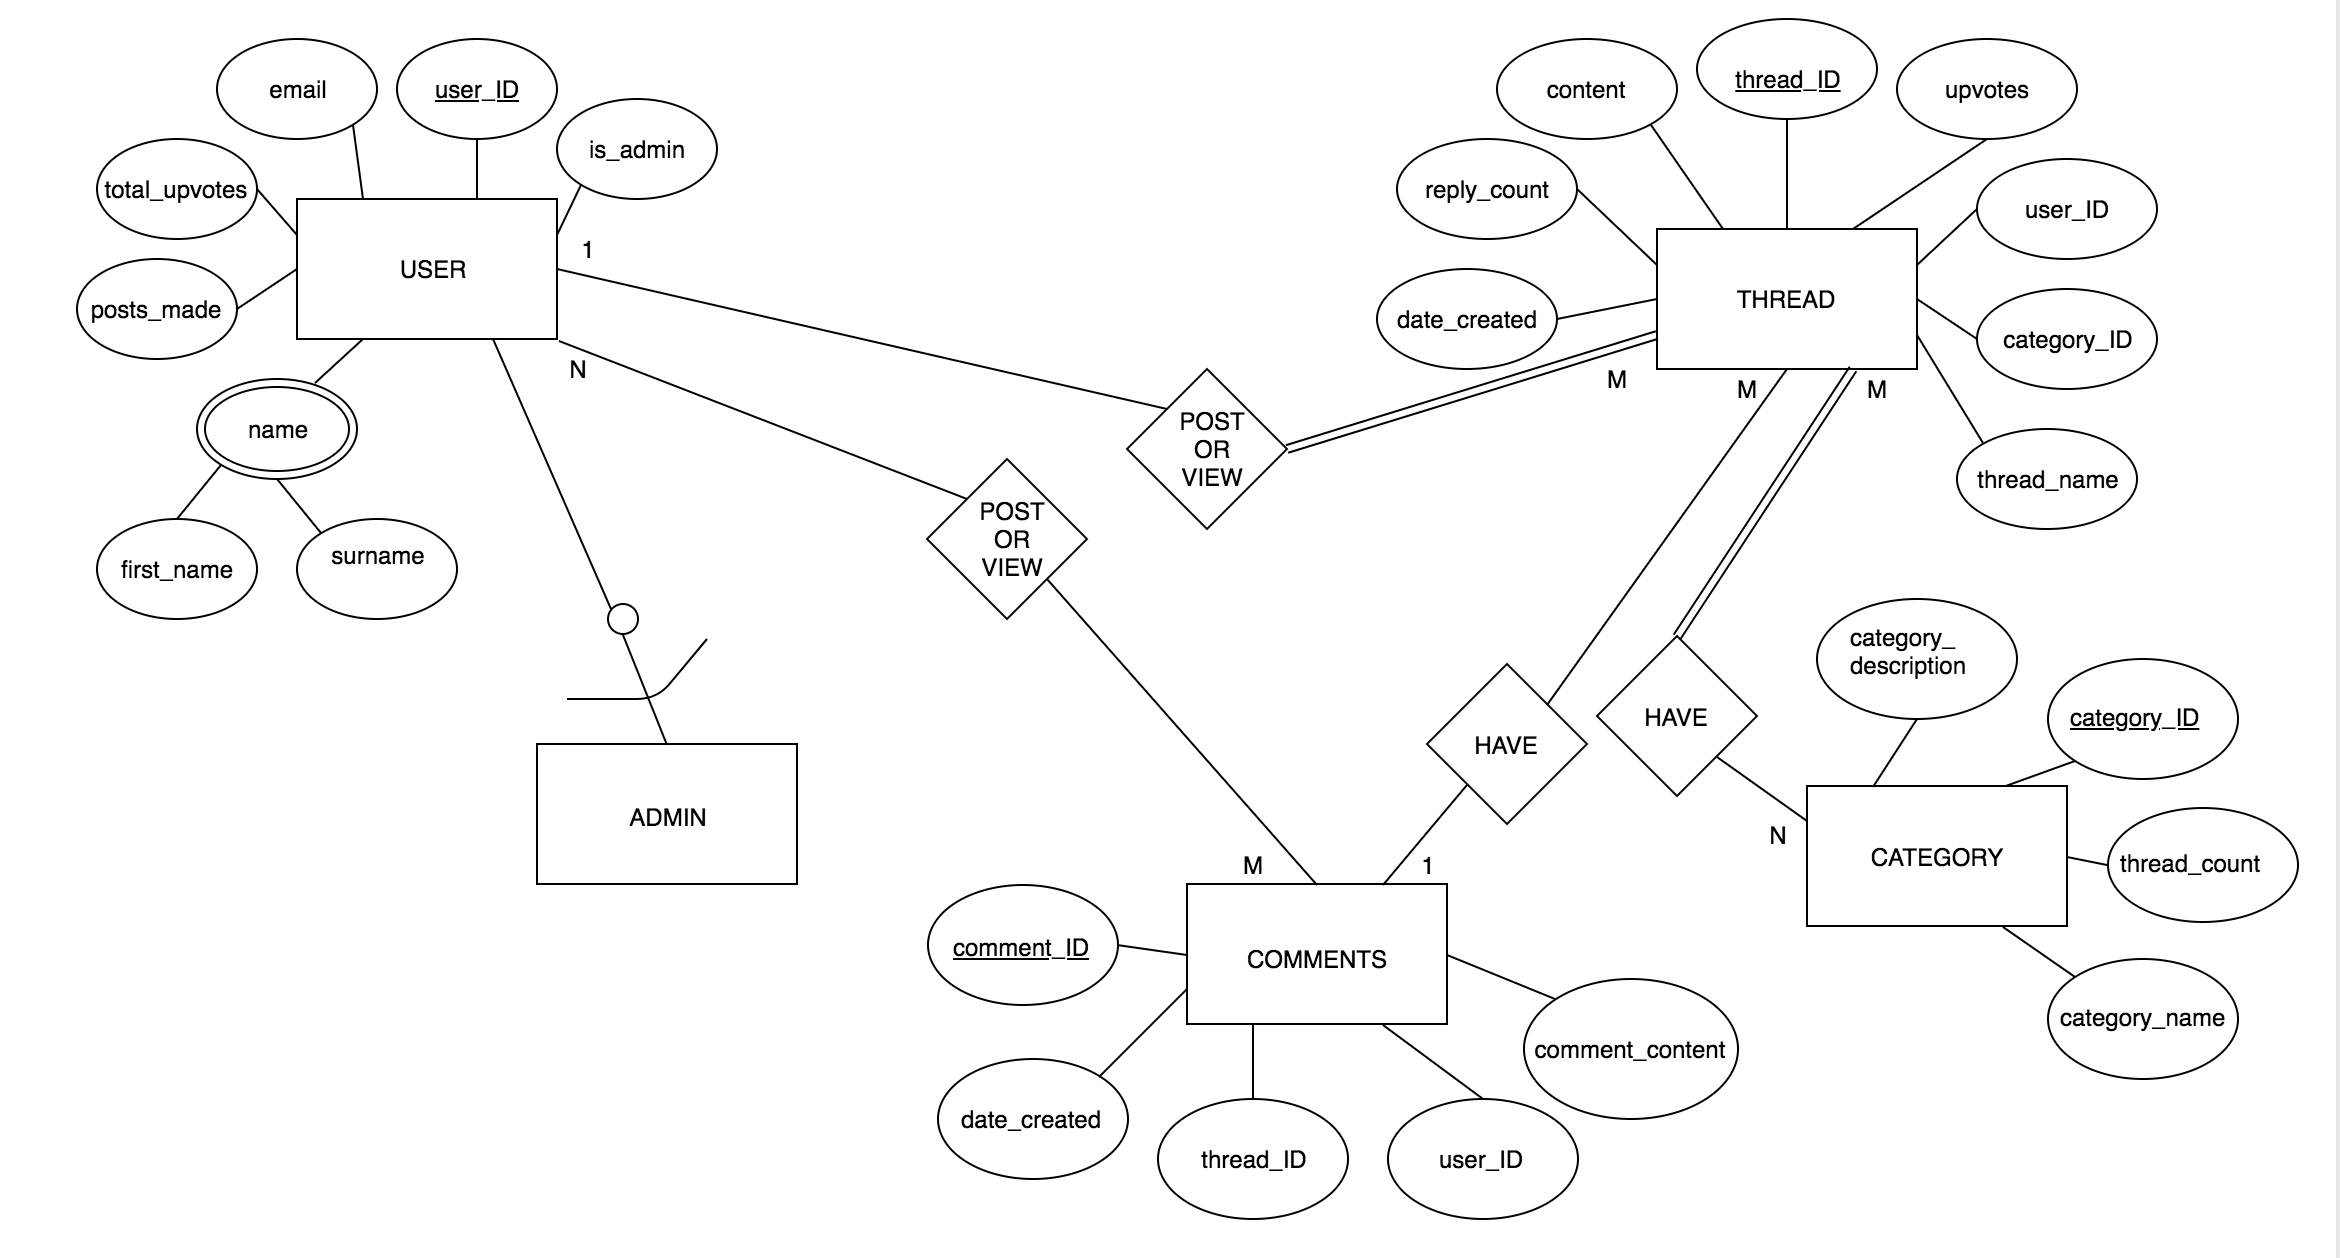
\includegraphics[width=\textwidth,height=\textheight,keepaspectratio]{er-dia}
\end{frame}

\begin{frame}
	\frametitle{Database Data Types - User}
	\begin{itemize}
		\item user\_ID (VARVCHAR) – the unique identifier for each registered user.
		\item Firstname/surname (VARCHAR) – the first and last name of the user.
		\item Email (VARCHAR) – the users email address.
		\item Total\_upvotes (INT) – the total number of upvotes that user has accumulated from all their posts.
		\item Posts\-made(INT) – the total number of posts the user has made.
		\item Is\_admin (BOOLEAN) – the status of the user (if they are an admin or not).
	\end{itemize}
\end{frame}

\begin{frame}
	\frametitle{Database Data Types - Thread}
	\begin{itemize}
		\item Thread\_ID (VARCHAR) – the unique identifier of the thread.
		\item Thread\_name (VARCHAR) – the name of the thread.
		\item Thread\_Content (VARCHAR) – the content that the poster uploads (i.e. the deal).
		\item Reply\_count (INT) – the number of replies the thread has.
		\item Date\_created (INT) – the date when the thread was created.
		\item Upvotes (INT) – the number of upvotes the thread has.
	\end{itemize}
\end{frame}

\begin{frame}
	\frametitle{Database Data Types - Category}
	\begin{itemize}
		\item Category\_ID (VARCHAR) – the unique identifier of the category.
		\item Category\_name (VARCHAR) – the name of the category.
		\item Thread\_count (INT) – the number of threads within the category.
		\item Category\_description (VARCHAR) – a description of what the category is.
	\end{itemize}
\end{frame}

\begin{frame}
	\frametitle{Databse Data Types - Comment}
	\begin{itemize}
		\item Comment\_ID – the unique identifier for each comment.
		\item Date\_created (INT) – the date in which the comment was created.
		\item Comment\_content (VARCHAR) – the comment left itself.
	\end{itemize}
\end{frame}

\begin{frame}
	\frametitle{Wireframe - Index}
	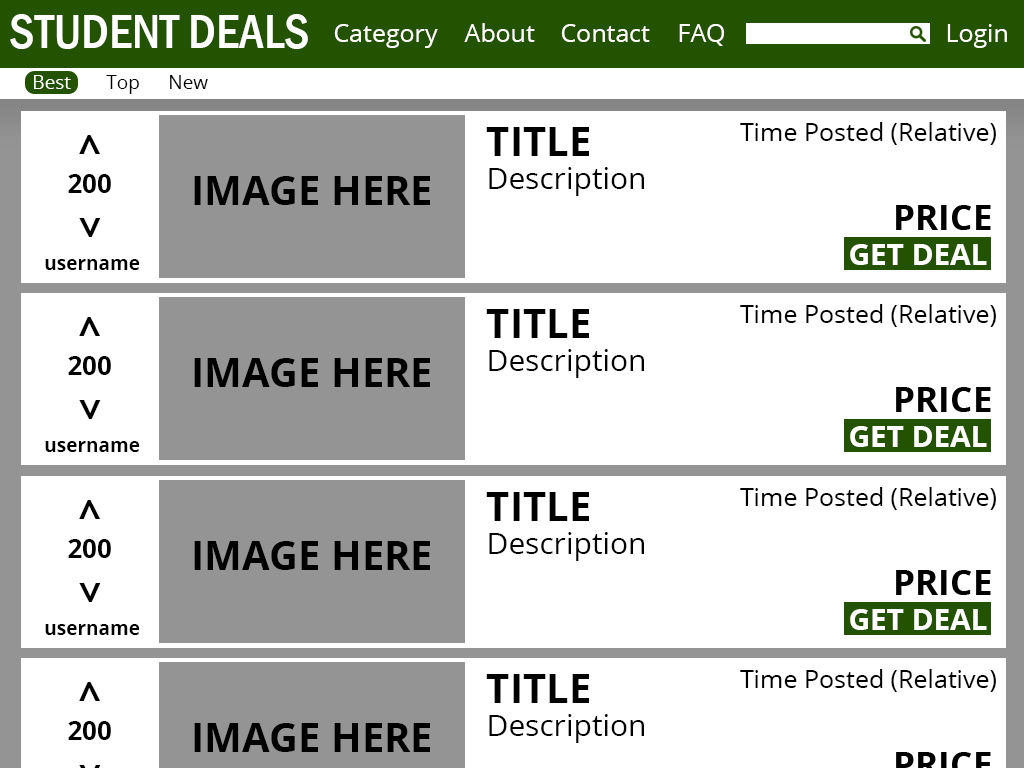
\includegraphics[width=\textwidth,height=\textheight,keepaspectratio]{mockups/index}
\end{frame}

\begin{frame}
	\frametitle{Wireframe - Deal Page}
	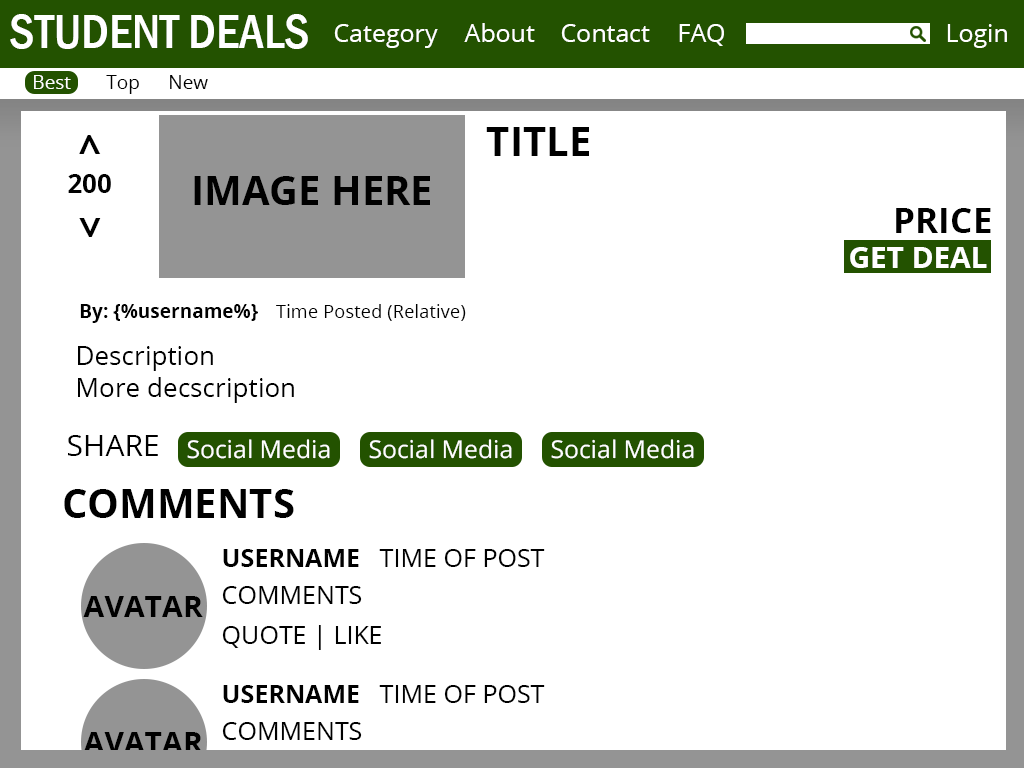
\includegraphics[width=\textwidth,height=\textheight,keepaspectratio]{mockups/deal-page}
\end{frame}

\begin{frame}
	\frametitle{Wireframe - Login}
	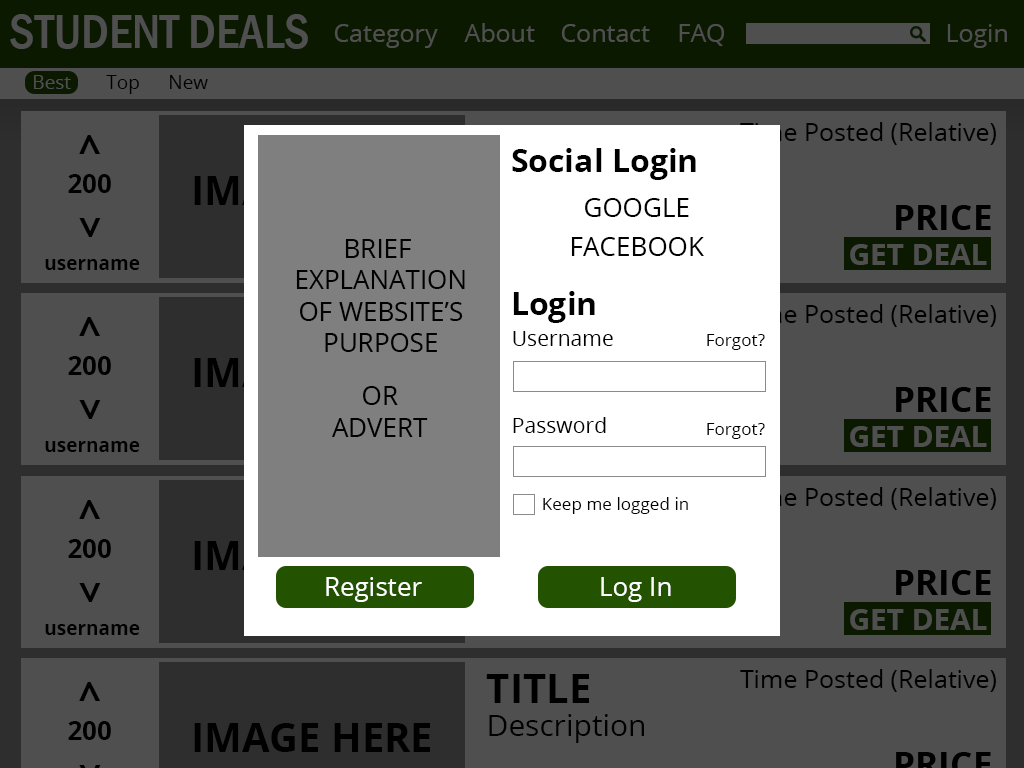
\includegraphics[width=\textwidth,height=\textheight,keepaspectratio]{mockups/login}
\end{frame}
	
\begin{frame}
	\frametitle{Sitemap}
	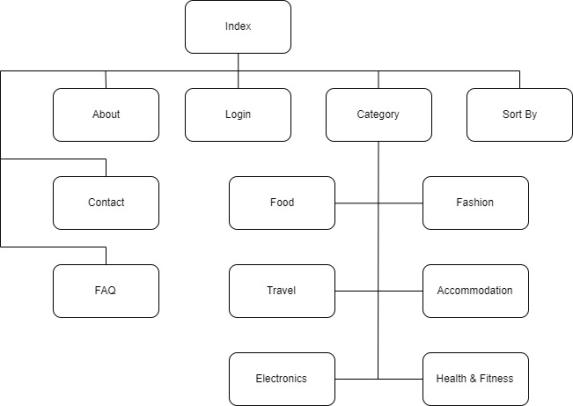
\includegraphics[width=\textwidth,height=\textheight,keepaspectratio]{site-map.jpg}
\end{frame}

\end{document}
